\documentclass[twoside]{book}

% Packages required by doxygen
\usepackage{fixltx2e}
\usepackage{calc}
\usepackage{doxygen}
\usepackage[export]{adjustbox} % also loads graphicx
\usepackage{graphicx}
\usepackage[utf8]{inputenc}
\usepackage{makeidx}
\usepackage{multicol}
\usepackage{multirow}
\PassOptionsToPackage{warn}{textcomp}
\usepackage{textcomp}
\usepackage[nointegrals]{wasysym}
\usepackage[table]{xcolor}

% Font selection
\usepackage[T1]{fontenc}
\usepackage[scaled=.90]{helvet}
\usepackage{courier}
\usepackage{amssymb}
\usepackage{sectsty}
\renewcommand{\familydefault}{\sfdefault}
\allsectionsfont{%
  \fontseries{bc}\selectfont%
  \color{darkgray}%
}
\renewcommand{\DoxyLabelFont}{%
  \fontseries{bc}\selectfont%
  \color{darkgray}%
}
\newcommand{\+}{\discretionary{\mbox{\scriptsize$\hookleftarrow$}}{}{}}

% Page & text layout
\usepackage{geometry}
\geometry{%
  a4paper,%
  top=2.5cm,%
  bottom=2.5cm,%
  left=2.5cm,%
  right=2.5cm%
}
\tolerance=750
\hfuzz=15pt
\hbadness=750
\setlength{\emergencystretch}{15pt}
\setlength{\parindent}{0cm}
\setlength{\parskip}{0.2cm}
\makeatletter
\renewcommand{\paragraph}{%
  \@startsection{paragraph}{4}{0ex}{-1.0ex}{1.0ex}{%
    \normalfont\normalsize\bfseries\SS@parafont%
  }%
}
\renewcommand{\subparagraph}{%
  \@startsection{subparagraph}{5}{0ex}{-1.0ex}{1.0ex}{%
    \normalfont\normalsize\bfseries\SS@subparafont%
  }%
}
\makeatother

% Headers & footers
\usepackage{fancyhdr}
\pagestyle{fancyplain}
\fancyhead[LE]{\fancyplain{}{\bfseries\thepage}}
\fancyhead[CE]{\fancyplain{}{}}
\fancyhead[RE]{\fancyplain{}{\bfseries\leftmark}}
\fancyhead[LO]{\fancyplain{}{\bfseries\rightmark}}
\fancyhead[CO]{\fancyplain{}{}}
\fancyhead[RO]{\fancyplain{}{\bfseries\thepage}}
\fancyfoot[LE]{\fancyplain{}{}}
\fancyfoot[CE]{\fancyplain{}{}}
\fancyfoot[RE]{\fancyplain{}{\bfseries\scriptsize Generated on Thu Dec 24 2015 03\+:03\+:28 for A\+E\+D\+A\+\_\+\+P\+R\+O\+J\+E\+C\+T\+O\+\_\+1 by Doxygen }}
\fancyfoot[LO]{\fancyplain{}{\bfseries\scriptsize Generated on Thu Dec 24 2015 03\+:03\+:28 for A\+E\+D\+A\+\_\+\+P\+R\+O\+J\+E\+C\+T\+O\+\_\+1 by Doxygen }}
\fancyfoot[CO]{\fancyplain{}{}}
\fancyfoot[RO]{\fancyplain{}{}}
\renewcommand{\footrulewidth}{0.4pt}
\renewcommand{\chaptermark}[1]{%
  \markboth{#1}{}%
}
\renewcommand{\sectionmark}[1]{%
  \markright{\thesection\ #1}%
}

% Indices & bibliography
\usepackage{natbib}
\usepackage[titles]{tocloft}
\setcounter{tocdepth}{3}
\setcounter{secnumdepth}{5}
\makeindex

% Hyperlinks (required, but should be loaded last)
\usepackage{ifpdf}
\ifpdf
  \usepackage[pdftex,pagebackref=true]{hyperref}
\else
  \usepackage[ps2pdf,pagebackref=true]{hyperref}
\fi
\hypersetup{%
  colorlinks=true,%
  linkcolor=blue,%
  citecolor=blue,%
  unicode%
}

% Custom commands
\newcommand{\clearemptydoublepage}{%
  \newpage{\pagestyle{empty}\cleardoublepage}%
}


%===== C O N T E N T S =====

\begin{document}

% Titlepage & ToC
\hypersetup{pageanchor=false,
             bookmarks=true,
             bookmarksnumbered=true,
             pdfencoding=unicode
            }
\pagenumbering{roman}
\begin{titlepage}
\vspace*{7cm}
\begin{center}%
{\Large A\+E\+D\+A\+\_\+\+P\+R\+O\+J\+E\+C\+T\+O\+\_\+1 }\\
\vspace*{1cm}
{\large Generated by Doxygen 1.8.10}\\
\vspace*{0.5cm}
{\small Thu Dec 24 2015 03:03:28}\\
\end{center}
\end{titlepage}
\clearemptydoublepage
\tableofcontents
\clearemptydoublepage
\pagenumbering{arabic}
\hypersetup{pageanchor=true}

%--- Begin generated contents ---
\chapter{Hierarchical Index}
\section{Class Hierarchy}
This inheritance list is sorted roughly, but not completely, alphabetically\+:\begin{DoxyCompactList}
\item \contentsline{section}{Atleta}{\pageref{class_atleta}}{}
\item \contentsline{section}{Atleta\+Inexistente}{\pageref{class_atleta_inexistente}}{}
\item \contentsline{section}{Calendario}{\pageref{class_calendario}}{}
\item \contentsline{section}{Campeonato}{\pageref{class_campeonato}}{}
\item \contentsline{section}{date}{\pageref{structdate}}{}
\item \contentsline{section}{Desporto}{\pageref{class_desporto}}{}
\begin{DoxyCompactList}
\item \contentsline{section}{Modalidade}{\pageref{class_modalidade}}{}
\end{DoxyCompactList}
\item \contentsline{section}{Equipa}{\pageref{class_equipa}}{}
\item \contentsline{section}{Equipa\+Inexistente}{\pageref{class_equipa_inexistente}}{}
\item \contentsline{section}{Erro\+No\+Ficheiro}{\pageref{class_erro_no_ficheiro}}{}
\item \contentsline{section}{info}{\pageref{structinfo}}{}
\item \contentsline{section}{Participante\+Inexistente}{\pageref{class_participante_inexistente}}{}
\item \contentsline{section}{Prova}{\pageref{class_prova}}{}
\item \contentsline{section}{Prova\+Inexistente}{\pageref{class_prova_inexistente}}{}
\item \contentsline{section}{Valor\+Invalido}{\pageref{class_valor_invalido}}{}
\end{DoxyCompactList}

\chapter{Class Index}
\section{Class List}
Here are the classes, structs, unions and interfaces with brief descriptions\+:\begin{DoxyCompactList}
\item\contentsline{section}{\hyperlink{class_atleta}{Atleta} }{\pageref{class_atleta}}{}
\item\contentsline{section}{\hyperlink{class_atleta_inexistente}{Atleta\+Inexistente} }{\pageref{class_atleta_inexistente}}{}
\item\contentsline{section}{\hyperlink{class_calendario}{Calendario} }{\pageref{class_calendario}}{}
\item\contentsline{section}{\hyperlink{class_campeonato}{Campeonato} }{\pageref{class_campeonato}}{}
\item\contentsline{section}{\hyperlink{structdate}{date} }{\pageref{structdate}}{}
\item\contentsline{section}{\hyperlink{class_desporto}{Desporto} }{\pageref{class_desporto}}{}
\item\contentsline{section}{\hyperlink{class_equipa}{Equipa} }{\pageref{class_equipa}}{}
\item\contentsline{section}{\hyperlink{class_equipa_inexistente}{Equipa\+Inexistente} }{\pageref{class_equipa_inexistente}}{}
\item\contentsline{section}{\hyperlink{class_erro_no_ficheiro}{Erro\+No\+Ficheiro} }{\pageref{class_erro_no_ficheiro}}{}
\item\contentsline{section}{\hyperlink{structinfo}{info} }{\pageref{structinfo}}{}
\item\contentsline{section}{\hyperlink{class_modalidade}{Modalidade} }{\pageref{class_modalidade}}{}
\item\contentsline{section}{\hyperlink{class_participante_nao_encontrado}{Participante\+Nao\+Encontrado} }{\pageref{class_participante_nao_encontrado}}{}
\item\contentsline{section}{\hyperlink{class_prova}{Prova} }{\pageref{class_prova}}{}
\item\contentsline{section}{\hyperlink{class_valor_invalido}{Valor\+Invalido} }{\pageref{class_valor_invalido}}{}
\end{DoxyCompactList}

\chapter{File Index}
\section{File List}
Here is a list of all files with brief descriptions\+:\begin{DoxyCompactList}
\item\contentsline{section}{C\+:/\+Users/\+Alexandre/\+Git\+Hub/\+A\+E\+D\+A\+\_\+\+P\+R\+O\+J\+E\+C\+T\+O\+\_\+1/src/logic/\hyperlink{_atleta_8cpp}{Atleta.\+cpp} }{\pageref{_atleta_8cpp}}{}
\item\contentsline{section}{C\+:/\+Users/\+Alexandre/\+Git\+Hub/\+A\+E\+D\+A\+\_\+\+P\+R\+O\+J\+E\+C\+T\+O\+\_\+1/src/logic/\hyperlink{_atleta_8h}{Atleta.\+h} }{\pageref{_atleta_8h}}{}
\item\contentsline{section}{C\+:/\+Users/\+Alexandre/\+Git\+Hub/\+A\+E\+D\+A\+\_\+\+P\+R\+O\+J\+E\+C\+T\+O\+\_\+1/src/logic/\hyperlink{_calendario_8cpp}{Calendario.\+cpp} }{\pageref{_calendario_8cpp}}{}
\item\contentsline{section}{C\+:/\+Users/\+Alexandre/\+Git\+Hub/\+A\+E\+D\+A\+\_\+\+P\+R\+O\+J\+E\+C\+T\+O\+\_\+1/src/logic/\hyperlink{_calendario_8h}{Calendario.\+h} }{\pageref{_calendario_8h}}{}
\item\contentsline{section}{C\+:/\+Users/\+Alexandre/\+Git\+Hub/\+A\+E\+D\+A\+\_\+\+P\+R\+O\+J\+E\+C\+T\+O\+\_\+1/src/logic/\hyperlink{_campeonato_8cpp}{Campeonato.\+cpp} }{\pageref{_campeonato_8cpp}}{}
\item\contentsline{section}{C\+:/\+Users/\+Alexandre/\+Git\+Hub/\+A\+E\+D\+A\+\_\+\+P\+R\+O\+J\+E\+C\+T\+O\+\_\+1/src/logic/\hyperlink{_campeonato_8h}{Campeonato.\+h} }{\pageref{_campeonato_8h}}{}
\item\contentsline{section}{C\+:/\+Users/\+Alexandre/\+Git\+Hub/\+A\+E\+D\+A\+\_\+\+P\+R\+O\+J\+E\+C\+T\+O\+\_\+1/src/logic/\hyperlink{_desporto_8h}{Desporto.\+h} }{\pageref{_desporto_8h}}{}
\item\contentsline{section}{C\+:/\+Users/\+Alexandre/\+Git\+Hub/\+A\+E\+D\+A\+\_\+\+P\+R\+O\+J\+E\+C\+T\+O\+\_\+1/src/logic/\hyperlink{_equipa_8cpp}{Equipa.\+cpp} }{\pageref{_equipa_8cpp}}{}
\item\contentsline{section}{C\+:/\+Users/\+Alexandre/\+Git\+Hub/\+A\+E\+D\+A\+\_\+\+P\+R\+O\+J\+E\+C\+T\+O\+\_\+1/src/logic/\hyperlink{_equipa_8h}{Equipa.\+h} }{\pageref{_equipa_8h}}{}
\item\contentsline{section}{C\+:/\+Users/\+Alexandre/\+Git\+Hub/\+A\+E\+D\+A\+\_\+\+P\+R\+O\+J\+E\+C\+T\+O\+\_\+1/src/logic/\hyperlink{main_8cpp}{main.\+cpp} }{\pageref{main_8cpp}}{}
\item\contentsline{section}{C\+:/\+Users/\+Alexandre/\+Git\+Hub/\+A\+E\+D\+A\+\_\+\+P\+R\+O\+J\+E\+C\+T\+O\+\_\+1/src/logic/\hyperlink{main_8h}{main.\+h} }{\pageref{main_8h}}{}
\item\contentsline{section}{C\+:/\+Users/\+Alexandre/\+Git\+Hub/\+A\+E\+D\+A\+\_\+\+P\+R\+O\+J\+E\+C\+T\+O\+\_\+1/src/logic/\hyperlink{_modalidade_8cpp}{Modalidade.\+cpp} }{\pageref{_modalidade_8cpp}}{}
\item\contentsline{section}{C\+:/\+Users/\+Alexandre/\+Git\+Hub/\+A\+E\+D\+A\+\_\+\+P\+R\+O\+J\+E\+C\+T\+O\+\_\+1/src/logic/\hyperlink{_modalidade_8h}{Modalidade.\+h} }{\pageref{_modalidade_8h}}{}
\item\contentsline{section}{C\+:/\+Users/\+Alexandre/\+Git\+Hub/\+A\+E\+D\+A\+\_\+\+P\+R\+O\+J\+E\+C\+T\+O\+\_\+1/src/logic/\hyperlink{_prova_8cpp}{Prova.\+cpp} }{\pageref{_prova_8cpp}}{}
\item\contentsline{section}{C\+:/\+Users/\+Alexandre/\+Git\+Hub/\+A\+E\+D\+A\+\_\+\+P\+R\+O\+J\+E\+C\+T\+O\+\_\+1/src/logic/\hyperlink{_prova_8h}{Prova.\+h} }{\pageref{_prova_8h}}{}
\item\contentsline{section}{C\+:/\+Users/\+Alexandre/\+Git\+Hub/\+A\+E\+D\+A\+\_\+\+P\+R\+O\+J\+E\+C\+T\+O\+\_\+1/src/logic/\hyperlink{_utilities_8h}{Utilities.\+h} }{\pageref{_utilities_8h}}{}
\end{DoxyCompactList}

\chapter{Class Documentation}
\hypertarget{class_adepto}{}\section{Adepto Class Reference}
\label{class_adepto}\index{Adepto@{Adepto}}


{\ttfamily \#include $<$Adepto.\+h$>$}

\subsection*{Public Member Functions}
\begin{DoxyCompactItemize}
\item 
\hyperlink{class_adepto_a544f7724e93beda5d7894ebb75aa5b38}{Adepto} (string \hyperlink{class_adepto_affdc168657d04f7c3622fda86815e195}{nome}, string \hyperlink{class_adepto_aad262806f93b5370f0619176929b8c2a}{email}, string n\+Eq)
\item 
\hyperlink{class_adepto_a3837c098f59e89d052cc74ce609d10d2}{Adepto} ()
\item 
\hyperlink{class_adepto_abf3f3fd153f85c802b709bba8f68b9f3}{Adepto} (string \hyperlink{class_adepto_affdc168657d04f7c3622fda86815e195}{nome})
\item 
unsigned int \hyperlink{class_adepto_a4fb9b0cd25432702e9bf4bc1594774c1}{get\+I\+D} () const 
\item 
string \hyperlink{class_adepto_aa655b5b5e1dcc07819d76140e69e0253}{get\+Nome} () const 
\item 
void \hyperlink{class_adepto_aa9e32095e7df2fd36397fed0ce703c58}{set\+Nome} (string n)
\item 
string \hyperlink{class_adepto_a89f0d930bde1684922ab7f75ae4a20a3}{get\+Equipa} () const 
\item 
void \hyperlink{class_adepto_a04d6c7667c430ae34e86e6ecbe0d8c1d}{set\+Equipa} (string n\+Eq)
\item 
string \hyperlink{class_adepto_ad3244a84912f4ff2034764f8c1a887d4}{get\+Email} () const 
\item 
void \hyperlink{class_adepto_a9c041dbfb8f2b822bb987e752996ce10}{set\+Email} (string novo\+Email)
\item 
void \hyperlink{class_adepto_ab10a21b804436408331e35b1c964ecee}{inserir\+Adepto} (\hyperlink{class_adepto}{Adepto} \&ad)
\item 
string \hyperlink{class_adepto_a345a20624756c6d52880a71f104d30ce}{get\+Info} () const 
\item 
void \hyperlink{class_adepto_a91073cf4e3d3044495d126e876533362}{imprime} () const 
\item 
bool \hyperlink{class_adepto_aac3192ff5a2aca2008d1393500a3bd00}{operator==} (const \hyperlink{class_adepto}{Adepto} \&a1)
\end{DoxyCompactItemize}
\subsection*{Private Attributes}
\begin{DoxyCompactItemize}
\item 
int \hyperlink{class_adepto_a63a2ece257caf45c0c8ec6d04c19fe0b}{uid}
\item 
string \hyperlink{class_adepto_aad262806f93b5370f0619176929b8c2a}{email}
\item 
string \hyperlink{class_adepto_affdc168657d04f7c3622fda86815e195}{nome}
\item 
string \hyperlink{class_adepto_a4d306b827599faf2eef7c6aee28c2a7f}{n\+Equipa}
\end{DoxyCompactItemize}
\subsection*{Static Private Attributes}
\begin{DoxyCompactItemize}
\item 
static int \hyperlink{class_adepto_a1255efa082f32bc2bab9fbe0790776aa}{new\+I\+D} = 0
\end{DoxyCompactItemize}


\subsection{Constructor \& Destructor Documentation}
\hypertarget{class_adepto_a544f7724e93beda5d7894ebb75aa5b38}{}\index{Adepto@{Adepto}!Adepto@{Adepto}}
\index{Adepto@{Adepto}!Adepto@{Adepto}}
\subsubsection[{Adepto(string nome, string email, string n\+Eq)}]{\setlength{\rightskip}{0pt plus 5cm}Adepto\+::\+Adepto (
\begin{DoxyParamCaption}
\item[{string}]{nome, }
\item[{string}]{email, }
\item[{string}]{n\+Eq}
\end{DoxyParamCaption}
)}\label{class_adepto_a544f7724e93beda5d7894ebb75aa5b38}
\hypertarget{class_adepto_a3837c098f59e89d052cc74ce609d10d2}{}\index{Adepto@{Adepto}!Adepto@{Adepto}}
\index{Adepto@{Adepto}!Adepto@{Adepto}}
\subsubsection[{Adepto()}]{\setlength{\rightskip}{0pt plus 5cm}Adepto\+::\+Adepto (
\begin{DoxyParamCaption}
{}
\end{DoxyParamCaption}
)}\label{class_adepto_a3837c098f59e89d052cc74ce609d10d2}
\hypertarget{class_adepto_abf3f3fd153f85c802b709bba8f68b9f3}{}\index{Adepto@{Adepto}!Adepto@{Adepto}}
\index{Adepto@{Adepto}!Adepto@{Adepto}}
\subsubsection[{Adepto(string nome)}]{\setlength{\rightskip}{0pt plus 5cm}Adepto\+::\+Adepto (
\begin{DoxyParamCaption}
\item[{string}]{nome}
\end{DoxyParamCaption}
)}\label{class_adepto_abf3f3fd153f85c802b709bba8f68b9f3}


\subsection{Member Function Documentation}
\hypertarget{class_adepto_ad3244a84912f4ff2034764f8c1a887d4}{}\index{Adepto@{Adepto}!get\+Email@{get\+Email}}
\index{get\+Email@{get\+Email}!Adepto@{Adepto}}
\subsubsection[{get\+Email() const }]{\setlength{\rightskip}{0pt plus 5cm}string Adepto\+::get\+Email (
\begin{DoxyParamCaption}
{}
\end{DoxyParamCaption}
) const}\label{class_adepto_ad3244a84912f4ff2034764f8c1a887d4}
\hypertarget{class_adepto_a89f0d930bde1684922ab7f75ae4a20a3}{}\index{Adepto@{Adepto}!get\+Equipa@{get\+Equipa}}
\index{get\+Equipa@{get\+Equipa}!Adepto@{Adepto}}
\subsubsection[{get\+Equipa() const }]{\setlength{\rightskip}{0pt plus 5cm}string Adepto\+::get\+Equipa (
\begin{DoxyParamCaption}
{}
\end{DoxyParamCaption}
) const}\label{class_adepto_a89f0d930bde1684922ab7f75ae4a20a3}
\hypertarget{class_adepto_a4fb9b0cd25432702e9bf4bc1594774c1}{}\index{Adepto@{Adepto}!get\+I\+D@{get\+I\+D}}
\index{get\+I\+D@{get\+I\+D}!Adepto@{Adepto}}
\subsubsection[{get\+I\+D() const }]{\setlength{\rightskip}{0pt plus 5cm}unsigned int Adepto\+::get\+I\+D (
\begin{DoxyParamCaption}
{}
\end{DoxyParamCaption}
) const}\label{class_adepto_a4fb9b0cd25432702e9bf4bc1594774c1}
\hypertarget{class_adepto_a345a20624756c6d52880a71f104d30ce}{}\index{Adepto@{Adepto}!get\+Info@{get\+Info}}
\index{get\+Info@{get\+Info}!Adepto@{Adepto}}
\subsubsection[{get\+Info() const }]{\setlength{\rightskip}{0pt plus 5cm}string Adepto\+::get\+Info (
\begin{DoxyParamCaption}
{}
\end{DoxyParamCaption}
) const}\label{class_adepto_a345a20624756c6d52880a71f104d30ce}
\hypertarget{class_adepto_aa655b5b5e1dcc07819d76140e69e0253}{}\index{Adepto@{Adepto}!get\+Nome@{get\+Nome}}
\index{get\+Nome@{get\+Nome}!Adepto@{Adepto}}
\subsubsection[{get\+Nome() const }]{\setlength{\rightskip}{0pt plus 5cm}string Adepto\+::get\+Nome (
\begin{DoxyParamCaption}
{}
\end{DoxyParamCaption}
) const}\label{class_adepto_aa655b5b5e1dcc07819d76140e69e0253}
\hypertarget{class_adepto_a91073cf4e3d3044495d126e876533362}{}\index{Adepto@{Adepto}!imprime@{imprime}}
\index{imprime@{imprime}!Adepto@{Adepto}}
\subsubsection[{imprime() const }]{\setlength{\rightskip}{0pt plus 5cm}void Adepto\+::imprime (
\begin{DoxyParamCaption}
{}
\end{DoxyParamCaption}
) const}\label{class_adepto_a91073cf4e3d3044495d126e876533362}
\hypertarget{class_adepto_ab10a21b804436408331e35b1c964ecee}{}\index{Adepto@{Adepto}!inserir\+Adepto@{inserir\+Adepto}}
\index{inserir\+Adepto@{inserir\+Adepto}!Adepto@{Adepto}}
\subsubsection[{inserir\+Adepto(\+Adepto \&ad)}]{\setlength{\rightskip}{0pt plus 5cm}void Adepto\+::inserir\+Adepto (
\begin{DoxyParamCaption}
\item[{{\bf Adepto} \&}]{ad}
\end{DoxyParamCaption}
)}\label{class_adepto_ab10a21b804436408331e35b1c964ecee}
\hypertarget{class_adepto_aac3192ff5a2aca2008d1393500a3bd00}{}\index{Adepto@{Adepto}!operator==@{operator==}}
\index{operator==@{operator==}!Adepto@{Adepto}}
\subsubsection[{operator==(const Adepto \&a1)}]{\setlength{\rightskip}{0pt plus 5cm}bool Adepto\+::operator== (
\begin{DoxyParamCaption}
\item[{const {\bf Adepto} \&}]{a1}
\end{DoxyParamCaption}
)}\label{class_adepto_aac3192ff5a2aca2008d1393500a3bd00}
\hypertarget{class_adepto_a9c041dbfb8f2b822bb987e752996ce10}{}\index{Adepto@{Adepto}!set\+Email@{set\+Email}}
\index{set\+Email@{set\+Email}!Adepto@{Adepto}}
\subsubsection[{set\+Email(string novo\+Email)}]{\setlength{\rightskip}{0pt plus 5cm}void Adepto\+::set\+Email (
\begin{DoxyParamCaption}
\item[{string}]{novo\+Email}
\end{DoxyParamCaption}
)}\label{class_adepto_a9c041dbfb8f2b822bb987e752996ce10}
\hypertarget{class_adepto_a04d6c7667c430ae34e86e6ecbe0d8c1d}{}\index{Adepto@{Adepto}!set\+Equipa@{set\+Equipa}}
\index{set\+Equipa@{set\+Equipa}!Adepto@{Adepto}}
\subsubsection[{set\+Equipa(string n\+Eq)}]{\setlength{\rightskip}{0pt plus 5cm}void Adepto\+::set\+Equipa (
\begin{DoxyParamCaption}
\item[{string}]{n\+Eq}
\end{DoxyParamCaption}
)}\label{class_adepto_a04d6c7667c430ae34e86e6ecbe0d8c1d}
\hypertarget{class_adepto_aa9e32095e7df2fd36397fed0ce703c58}{}\index{Adepto@{Adepto}!set\+Nome@{set\+Nome}}
\index{set\+Nome@{set\+Nome}!Adepto@{Adepto}}
\subsubsection[{set\+Nome(string n)}]{\setlength{\rightskip}{0pt plus 5cm}void Adepto\+::set\+Nome (
\begin{DoxyParamCaption}
\item[{string}]{n}
\end{DoxyParamCaption}
)}\label{class_adepto_aa9e32095e7df2fd36397fed0ce703c58}


\subsection{Member Data Documentation}
\hypertarget{class_adepto_aad262806f93b5370f0619176929b8c2a}{}\index{Adepto@{Adepto}!email@{email}}
\index{email@{email}!Adepto@{Adepto}}
\subsubsection[{email}]{\setlength{\rightskip}{0pt plus 5cm}string Adepto\+::email\hspace{0.3cm}{\ttfamily [private]}}\label{class_adepto_aad262806f93b5370f0619176929b8c2a}
\hypertarget{class_adepto_a4d306b827599faf2eef7c6aee28c2a7f}{}\index{Adepto@{Adepto}!n\+Equipa@{n\+Equipa}}
\index{n\+Equipa@{n\+Equipa}!Adepto@{Adepto}}
\subsubsection[{n\+Equipa}]{\setlength{\rightskip}{0pt plus 5cm}string Adepto\+::n\+Equipa\hspace{0.3cm}{\ttfamily [private]}}\label{class_adepto_a4d306b827599faf2eef7c6aee28c2a7f}
\hypertarget{class_adepto_a1255efa082f32bc2bab9fbe0790776aa}{}\index{Adepto@{Adepto}!new\+I\+D@{new\+I\+D}}
\index{new\+I\+D@{new\+I\+D}!Adepto@{Adepto}}
\subsubsection[{new\+I\+D}]{\setlength{\rightskip}{0pt plus 5cm}int Adepto\+::new\+I\+D = 0\hspace{0.3cm}{\ttfamily [static]}, {\ttfamily [private]}}\label{class_adepto_a1255efa082f32bc2bab9fbe0790776aa}
\hypertarget{class_adepto_affdc168657d04f7c3622fda86815e195}{}\index{Adepto@{Adepto}!nome@{nome}}
\index{nome@{nome}!Adepto@{Adepto}}
\subsubsection[{nome}]{\setlength{\rightskip}{0pt plus 5cm}string Adepto\+::nome\hspace{0.3cm}{\ttfamily [private]}}\label{class_adepto_affdc168657d04f7c3622fda86815e195}
\hypertarget{class_adepto_a63a2ece257caf45c0c8ec6d04c19fe0b}{}\index{Adepto@{Adepto}!uid@{uid}}
\index{uid@{uid}!Adepto@{Adepto}}
\subsubsection[{uid}]{\setlength{\rightskip}{0pt plus 5cm}int Adepto\+::uid\hspace{0.3cm}{\ttfamily [private]}}\label{class_adepto_a63a2ece257caf45c0c8ec6d04c19fe0b}


The documentation for this class was generated from the following files\+:\begin{DoxyCompactItemize}
\item 
C\+:/\+Users/\+Alexandre/\+Git\+Hub/\+A\+E\+D\+A\+\_\+\+P\+R\+O\+J\+E\+C\+T\+O\+\_\+1/src/logic/\hyperlink{_adepto_8h}{Adepto.\+h}\item 
C\+:/\+Users/\+Alexandre/\+Git\+Hub/\+A\+E\+D\+A\+\_\+\+P\+R\+O\+J\+E\+C\+T\+O\+\_\+1/src/logic/\hyperlink{_adepto_8cpp}{Adepto.\+cpp}\end{DoxyCompactItemize}

\hypertarget{class_adepto_inexistente}{}\section{Adepto\+Inexistente Class Reference}
\label{class_adepto_inexistente}\index{Adepto\+Inexistente@{Adepto\+Inexistente}}


{\ttfamily \#include $<$Utilities.\+h$>$}

\subsection*{Public Member Functions}
\begin{DoxyCompactItemize}
\item 
\hyperlink{class_adepto_inexistente_a2878cf170b9b750ca8beaa6ce3c30c4b}{Adepto\+Inexistente} (int \hyperlink{class_adepto_inexistente_ae58bcd6663bfa728a5c581b4befd2f25}{id})
\item 
\hyperlink{class_adepto_inexistente_a554e93ab0308ad692a76543401559e2b}{Adepto\+Inexistente} (string \hyperlink{class_adepto_inexistente_acaea652be13be5879b5fedb397a65634}{nome})
\item 
int \hyperlink{class_adepto_inexistente_a6dbe4bc4c8217bc6705c5dd2346ae77e}{get\+I\+D} ()
\item 
string \hyperlink{class_adepto_inexistente_a9c48a231fc680d29034877de0c838156}{get\+Nome} ()
\end{DoxyCompactItemize}
\subsection*{Public Attributes}
\begin{DoxyCompactItemize}
\item 
int \hyperlink{class_adepto_inexistente_ae58bcd6663bfa728a5c581b4befd2f25}{id}
\item 
string \hyperlink{class_adepto_inexistente_acaea652be13be5879b5fedb397a65634}{nome}
\end{DoxyCompactItemize}


\subsection{Constructor \& Destructor Documentation}
\hypertarget{class_adepto_inexistente_a2878cf170b9b750ca8beaa6ce3c30c4b}{}\index{Adepto\+Inexistente@{Adepto\+Inexistente}!Adepto\+Inexistente@{Adepto\+Inexistente}}
\index{Adepto\+Inexistente@{Adepto\+Inexistente}!Adepto\+Inexistente@{Adepto\+Inexistente}}
\subsubsection[{Adepto\+Inexistente(int id)}]{\setlength{\rightskip}{0pt plus 5cm}Adepto\+Inexistente\+::\+Adepto\+Inexistente (
\begin{DoxyParamCaption}
\item[{int}]{id}
\end{DoxyParamCaption}
)\hspace{0.3cm}{\ttfamily [inline]}}\label{class_adepto_inexistente_a2878cf170b9b750ca8beaa6ce3c30c4b}
\hypertarget{class_adepto_inexistente_a554e93ab0308ad692a76543401559e2b}{}\index{Adepto\+Inexistente@{Adepto\+Inexistente}!Adepto\+Inexistente@{Adepto\+Inexistente}}
\index{Adepto\+Inexistente@{Adepto\+Inexistente}!Adepto\+Inexistente@{Adepto\+Inexistente}}
\subsubsection[{Adepto\+Inexistente(string nome)}]{\setlength{\rightskip}{0pt plus 5cm}Adepto\+Inexistente\+::\+Adepto\+Inexistente (
\begin{DoxyParamCaption}
\item[{string}]{nome}
\end{DoxyParamCaption}
)\hspace{0.3cm}{\ttfamily [inline]}}\label{class_adepto_inexistente_a554e93ab0308ad692a76543401559e2b}


\subsection{Member Function Documentation}
\hypertarget{class_adepto_inexistente_a6dbe4bc4c8217bc6705c5dd2346ae77e}{}\index{Adepto\+Inexistente@{Adepto\+Inexistente}!get\+I\+D@{get\+I\+D}}
\index{get\+I\+D@{get\+I\+D}!Adepto\+Inexistente@{Adepto\+Inexistente}}
\subsubsection[{get\+I\+D()}]{\setlength{\rightskip}{0pt plus 5cm}int Adepto\+Inexistente\+::get\+I\+D (
\begin{DoxyParamCaption}
{}
\end{DoxyParamCaption}
)\hspace{0.3cm}{\ttfamily [inline]}}\label{class_adepto_inexistente_a6dbe4bc4c8217bc6705c5dd2346ae77e}
\hypertarget{class_adepto_inexistente_a9c48a231fc680d29034877de0c838156}{}\index{Adepto\+Inexistente@{Adepto\+Inexistente}!get\+Nome@{get\+Nome}}
\index{get\+Nome@{get\+Nome}!Adepto\+Inexistente@{Adepto\+Inexistente}}
\subsubsection[{get\+Nome()}]{\setlength{\rightskip}{0pt plus 5cm}string Adepto\+Inexistente\+::get\+Nome (
\begin{DoxyParamCaption}
{}
\end{DoxyParamCaption}
)\hspace{0.3cm}{\ttfamily [inline]}}\label{class_adepto_inexistente_a9c48a231fc680d29034877de0c838156}


\subsection{Member Data Documentation}
\hypertarget{class_adepto_inexistente_ae58bcd6663bfa728a5c581b4befd2f25}{}\index{Adepto\+Inexistente@{Adepto\+Inexistente}!id@{id}}
\index{id@{id}!Adepto\+Inexistente@{Adepto\+Inexistente}}
\subsubsection[{id}]{\setlength{\rightskip}{0pt plus 5cm}int Adepto\+Inexistente\+::id}\label{class_adepto_inexistente_ae58bcd6663bfa728a5c581b4befd2f25}
\hypertarget{class_adepto_inexistente_acaea652be13be5879b5fedb397a65634}{}\index{Adepto\+Inexistente@{Adepto\+Inexistente}!nome@{nome}}
\index{nome@{nome}!Adepto\+Inexistente@{Adepto\+Inexistente}}
\subsubsection[{nome}]{\setlength{\rightskip}{0pt plus 5cm}string Adepto\+Inexistente\+::nome}\label{class_adepto_inexistente_acaea652be13be5879b5fedb397a65634}


The documentation for this class was generated from the following file\+:\begin{DoxyCompactItemize}
\item 
C\+:/\+Users/\+Alexandre/\+Git\+Hub/\+A\+E\+D\+A\+\_\+\+P\+R\+O\+J\+E\+C\+T\+O\+\_\+1/src/logic/\hyperlink{_utilities_8h}{Utilities.\+h}\end{DoxyCompactItemize}

\hypertarget{class_atleta}{}\section{Atleta Class Reference}
\label{class_atleta}\index{Atleta@{Atleta}}


{\ttfamily \#include $<$Atleta.\+h$>$}

\subsection*{Public Member Functions}
\begin{DoxyCompactItemize}
\item 
\hyperlink{class_atleta_abd3d28e4321bd53ed8aa9c840a2278f1}{Atleta} (string n, string pais, unsigned int i, unsigned int p, unsigned int a)
\item 
\hyperlink{class_atleta_af1b4e011c71918d9c59b910afa88d64e}{Atleta} ()
\item 
\hyperlink{class_atleta_a6002feaeb345f754cdfde63987815dd2}{$\sim$\+Atleta} ()
\item 
unsigned int \hyperlink{class_atleta_a95ff067c6a7e3268425bfc97adf72171}{get\+I\+D} () const 
\item 
\hyperlink{structinfo}{info} \hyperlink{class_atleta_af8076b0fe0d69e6313685f1b3d7be27c}{get\+Info} () const 
\item 
void \hyperlink{class_atleta_ada229ccfc2a898c893c0a34c9c996892}{set\+Info} (\hyperlink{structinfo}{info} i)
\item 
string \hyperlink{class_atleta_a0f5be5cd0b18f224a7a5281216fc1bfd}{get\+Nome} () const 
\item 
void \hyperlink{class_atleta_a35fcdb190f9b6b5100fba23cc98e5304}{set\+Nome} (string n)
\item 
string \hyperlink{class_atleta_a6b19798bf0eca5caed86134b7932264d}{get\+Pais} () const 
\item 
void \hyperlink{class_atleta_a3a4c881326e44433537d44727d7d60de}{set\+Pais} (string p)
\item 
unsigned int \hyperlink{class_atleta_ad0a209bea90007c372d07465cb410fbc}{get\+Idade} () const 
\item 
void \hyperlink{class_atleta_a62b5097c74ad66181a05d6562c1a9a25}{set\+Idade} (int i)
\item 
unsigned int \hyperlink{class_atleta_aade1b300b0ed29445f63bed20392888c}{get\+Peso} () const 
\item 
void \hyperlink{class_atleta_af9ef31c49a31a7a4514f6c676caad01d}{set\+Peso} (int p)
\item 
unsigned int \hyperlink{class_atleta_a8ad4b5fcf8bb3cf4bdf6f428728c5ebc}{get\+Altura} () const 
\item 
void \hyperlink{class_atleta_a559420bb8aa5e5ee881ffe284f24a7df}{set\+Altura} (int a)
\item 
float \hyperlink{class_atleta_afc8a2e69817d94c7dad61a66928d98f6}{get\+Pontuacao} () const 
\item 
void \hyperlink{class_atleta_a4bacfffad058d3437083a4a53fd2169c}{set\+Pontuacao} (float p)
\item 
string \hyperlink{class_atleta_a82922d79c0b9570022fc9a5c8e866394}{get\+Equipa} () const 
\item 
void \hyperlink{class_atleta_acfad68eb32ba1ee1485368f1c7dc8b3f}{set\+Equipa} (string equipa)
\item 
vector$<$ \hyperlink{class_modalidade}{Modalidade} $\ast$ $>$ \hyperlink{class_atleta_a4e4a08618d388c914705e4552bee3f00}{get\+Modalidades} () const 
\item 
void \hyperlink{class_atleta_abd96127243b44401924386b4d6e5ceea}{inserir\+Modalidade} (\hyperlink{class_modalidade}{Modalidade} \&mod1)
\item 
void \hyperlink{class_atleta_abfac40f3ca907a1b89152794a5a29f96}{imprime} () const 
\end{DoxyCompactItemize}
\subsection*{Private Attributes}
\begin{DoxyCompactItemize}
\item 
int \hyperlink{class_atleta_ae471f8c198a8a84275afa23598e03d44}{uid}
\item 
\hyperlink{structinfo}{info} \hyperlink{class_atleta_a1492a3f905e1915797e128b7e0be8017}{inf}
\item 
float \hyperlink{class_atleta_ac7fb325ccbe94fe9494d54da4c08b045}{pontuacao}
\item 
string \hyperlink{class_atleta_af159b255beef6455905f0c871355b1ee}{n\+Equipa}
\item 
vector$<$ \hyperlink{class_modalidade}{Modalidade} $\ast$ $>$ \hyperlink{class_atleta_a0f04a0dcd8724d10617db7b1e2482e1c}{modalidades}
\end{DoxyCompactItemize}
\subsection*{Static Private Attributes}
\begin{DoxyCompactItemize}
\item 
static int \hyperlink{class_atleta_af206b52d53b2e4c5dfd4fec66bf1965c}{new\+I\+D} = 0
\end{DoxyCompactItemize}


\subsection{Constructor \& Destructor Documentation}
\hypertarget{class_atleta_abd3d28e4321bd53ed8aa9c840a2278f1}{}\index{Atleta@{Atleta}!Atleta@{Atleta}}
\index{Atleta@{Atleta}!Atleta@{Atleta}}
\subsubsection[{Atleta(string n, string pais, unsigned int i, unsigned int p, unsigned int a)}]{\setlength{\rightskip}{0pt plus 5cm}Atleta\+::\+Atleta (
\begin{DoxyParamCaption}
\item[{string}]{n, }
\item[{string}]{pais, }
\item[{unsigned int}]{i, }
\item[{unsigned int}]{p, }
\item[{unsigned int}]{a}
\end{DoxyParamCaption}
)}\label{class_atleta_abd3d28e4321bd53ed8aa9c840a2278f1}
\hypertarget{class_atleta_af1b4e011c71918d9c59b910afa88d64e}{}\index{Atleta@{Atleta}!Atleta@{Atleta}}
\index{Atleta@{Atleta}!Atleta@{Atleta}}
\subsubsection[{Atleta()}]{\setlength{\rightskip}{0pt plus 5cm}Atleta\+::\+Atleta (
\begin{DoxyParamCaption}
{}
\end{DoxyParamCaption}
)}\label{class_atleta_af1b4e011c71918d9c59b910afa88d64e}
\hypertarget{class_atleta_a6002feaeb345f754cdfde63987815dd2}{}\index{Atleta@{Atleta}!````~Atleta@{$\sim$\+Atleta}}
\index{````~Atleta@{$\sim$\+Atleta}!Atleta@{Atleta}}
\subsubsection[{$\sim$\+Atleta()}]{\setlength{\rightskip}{0pt plus 5cm}Atleta\+::$\sim$\+Atleta (
\begin{DoxyParamCaption}
{}
\end{DoxyParamCaption}
)}\label{class_atleta_a6002feaeb345f754cdfde63987815dd2}


\subsection{Member Function Documentation}
\hypertarget{class_atleta_a8ad4b5fcf8bb3cf4bdf6f428728c5ebc}{}\index{Atleta@{Atleta}!get\+Altura@{get\+Altura}}
\index{get\+Altura@{get\+Altura}!Atleta@{Atleta}}
\subsubsection[{get\+Altura() const }]{\setlength{\rightskip}{0pt plus 5cm}unsigned int Atleta\+::get\+Altura (
\begin{DoxyParamCaption}
{}
\end{DoxyParamCaption}
) const}\label{class_atleta_a8ad4b5fcf8bb3cf4bdf6f428728c5ebc}
\hypertarget{class_atleta_a82922d79c0b9570022fc9a5c8e866394}{}\index{Atleta@{Atleta}!get\+Equipa@{get\+Equipa}}
\index{get\+Equipa@{get\+Equipa}!Atleta@{Atleta}}
\subsubsection[{get\+Equipa() const }]{\setlength{\rightskip}{0pt plus 5cm}string Atleta\+::get\+Equipa (
\begin{DoxyParamCaption}
{}
\end{DoxyParamCaption}
) const}\label{class_atleta_a82922d79c0b9570022fc9a5c8e866394}
\hypertarget{class_atleta_a95ff067c6a7e3268425bfc97adf72171}{}\index{Atleta@{Atleta}!get\+I\+D@{get\+I\+D}}
\index{get\+I\+D@{get\+I\+D}!Atleta@{Atleta}}
\subsubsection[{get\+I\+D() const }]{\setlength{\rightskip}{0pt plus 5cm}unsigned int Atleta\+::get\+I\+D (
\begin{DoxyParamCaption}
{}
\end{DoxyParamCaption}
) const}\label{class_atleta_a95ff067c6a7e3268425bfc97adf72171}
\hypertarget{class_atleta_ad0a209bea90007c372d07465cb410fbc}{}\index{Atleta@{Atleta}!get\+Idade@{get\+Idade}}
\index{get\+Idade@{get\+Idade}!Atleta@{Atleta}}
\subsubsection[{get\+Idade() const }]{\setlength{\rightskip}{0pt plus 5cm}unsigned int Atleta\+::get\+Idade (
\begin{DoxyParamCaption}
{}
\end{DoxyParamCaption}
) const}\label{class_atleta_ad0a209bea90007c372d07465cb410fbc}
\hypertarget{class_atleta_af8076b0fe0d69e6313685f1b3d7be27c}{}\index{Atleta@{Atleta}!get\+Info@{get\+Info}}
\index{get\+Info@{get\+Info}!Atleta@{Atleta}}
\subsubsection[{get\+Info() const }]{\setlength{\rightskip}{0pt plus 5cm}{\bf info} Atleta\+::get\+Info (
\begin{DoxyParamCaption}
{}
\end{DoxyParamCaption}
) const}\label{class_atleta_af8076b0fe0d69e6313685f1b3d7be27c}
\hypertarget{class_atleta_a4e4a08618d388c914705e4552bee3f00}{}\index{Atleta@{Atleta}!get\+Modalidades@{get\+Modalidades}}
\index{get\+Modalidades@{get\+Modalidades}!Atleta@{Atleta}}
\subsubsection[{get\+Modalidades() const }]{\setlength{\rightskip}{0pt plus 5cm}vector$<$ {\bf Modalidade} $\ast$ $>$ Atleta\+::get\+Modalidades (
\begin{DoxyParamCaption}
{}
\end{DoxyParamCaption}
) const}\label{class_atleta_a4e4a08618d388c914705e4552bee3f00}
\hypertarget{class_atleta_a0f5be5cd0b18f224a7a5281216fc1bfd}{}\index{Atleta@{Atleta}!get\+Nome@{get\+Nome}}
\index{get\+Nome@{get\+Nome}!Atleta@{Atleta}}
\subsubsection[{get\+Nome() const }]{\setlength{\rightskip}{0pt plus 5cm}string Atleta\+::get\+Nome (
\begin{DoxyParamCaption}
{}
\end{DoxyParamCaption}
) const}\label{class_atleta_a0f5be5cd0b18f224a7a5281216fc1bfd}
\hypertarget{class_atleta_a6b19798bf0eca5caed86134b7932264d}{}\index{Atleta@{Atleta}!get\+Pais@{get\+Pais}}
\index{get\+Pais@{get\+Pais}!Atleta@{Atleta}}
\subsubsection[{get\+Pais() const }]{\setlength{\rightskip}{0pt plus 5cm}string Atleta\+::get\+Pais (
\begin{DoxyParamCaption}
{}
\end{DoxyParamCaption}
) const}\label{class_atleta_a6b19798bf0eca5caed86134b7932264d}
\hypertarget{class_atleta_aade1b300b0ed29445f63bed20392888c}{}\index{Atleta@{Atleta}!get\+Peso@{get\+Peso}}
\index{get\+Peso@{get\+Peso}!Atleta@{Atleta}}
\subsubsection[{get\+Peso() const }]{\setlength{\rightskip}{0pt plus 5cm}unsigned int Atleta\+::get\+Peso (
\begin{DoxyParamCaption}
{}
\end{DoxyParamCaption}
) const}\label{class_atleta_aade1b300b0ed29445f63bed20392888c}
\hypertarget{class_atleta_afc8a2e69817d94c7dad61a66928d98f6}{}\index{Atleta@{Atleta}!get\+Pontuacao@{get\+Pontuacao}}
\index{get\+Pontuacao@{get\+Pontuacao}!Atleta@{Atleta}}
\subsubsection[{get\+Pontuacao() const }]{\setlength{\rightskip}{0pt plus 5cm}float Atleta\+::get\+Pontuacao (
\begin{DoxyParamCaption}
{}
\end{DoxyParamCaption}
) const}\label{class_atleta_afc8a2e69817d94c7dad61a66928d98f6}
\hypertarget{class_atleta_abfac40f3ca907a1b89152794a5a29f96}{}\index{Atleta@{Atleta}!imprime@{imprime}}
\index{imprime@{imprime}!Atleta@{Atleta}}
\subsubsection[{imprime() const }]{\setlength{\rightskip}{0pt plus 5cm}void Atleta\+::imprime (
\begin{DoxyParamCaption}
{}
\end{DoxyParamCaption}
) const}\label{class_atleta_abfac40f3ca907a1b89152794a5a29f96}
\hypertarget{class_atleta_abd96127243b44401924386b4d6e5ceea}{}\index{Atleta@{Atleta}!inserir\+Modalidade@{inserir\+Modalidade}}
\index{inserir\+Modalidade@{inserir\+Modalidade}!Atleta@{Atleta}}
\subsubsection[{inserir\+Modalidade(\+Modalidade \&mod1)}]{\setlength{\rightskip}{0pt plus 5cm}void Atleta\+::inserir\+Modalidade (
\begin{DoxyParamCaption}
\item[{{\bf Modalidade} \&}]{mod1}
\end{DoxyParamCaption}
)}\label{class_atleta_abd96127243b44401924386b4d6e5ceea}
\hypertarget{class_atleta_a559420bb8aa5e5ee881ffe284f24a7df}{}\index{Atleta@{Atleta}!set\+Altura@{set\+Altura}}
\index{set\+Altura@{set\+Altura}!Atleta@{Atleta}}
\subsubsection[{set\+Altura(int a)}]{\setlength{\rightskip}{0pt plus 5cm}void Atleta\+::set\+Altura (
\begin{DoxyParamCaption}
\item[{int}]{a}
\end{DoxyParamCaption}
)}\label{class_atleta_a559420bb8aa5e5ee881ffe284f24a7df}
\hypertarget{class_atleta_acfad68eb32ba1ee1485368f1c7dc8b3f}{}\index{Atleta@{Atleta}!set\+Equipa@{set\+Equipa}}
\index{set\+Equipa@{set\+Equipa}!Atleta@{Atleta}}
\subsubsection[{set\+Equipa(string equipa)}]{\setlength{\rightskip}{0pt plus 5cm}void Atleta\+::set\+Equipa (
\begin{DoxyParamCaption}
\item[{string}]{equipa}
\end{DoxyParamCaption}
)}\label{class_atleta_acfad68eb32ba1ee1485368f1c7dc8b3f}
\hypertarget{class_atleta_a62b5097c74ad66181a05d6562c1a9a25}{}\index{Atleta@{Atleta}!set\+Idade@{set\+Idade}}
\index{set\+Idade@{set\+Idade}!Atleta@{Atleta}}
\subsubsection[{set\+Idade(int i)}]{\setlength{\rightskip}{0pt plus 5cm}void Atleta\+::set\+Idade (
\begin{DoxyParamCaption}
\item[{int}]{i}
\end{DoxyParamCaption}
)}\label{class_atleta_a62b5097c74ad66181a05d6562c1a9a25}
\hypertarget{class_atleta_ada229ccfc2a898c893c0a34c9c996892}{}\index{Atleta@{Atleta}!set\+Info@{set\+Info}}
\index{set\+Info@{set\+Info}!Atleta@{Atleta}}
\subsubsection[{set\+Info(info i)}]{\setlength{\rightskip}{0pt plus 5cm}void Atleta\+::set\+Info (
\begin{DoxyParamCaption}
\item[{{\bf info}}]{i}
\end{DoxyParamCaption}
)}\label{class_atleta_ada229ccfc2a898c893c0a34c9c996892}
\hypertarget{class_atleta_a35fcdb190f9b6b5100fba23cc98e5304}{}\index{Atleta@{Atleta}!set\+Nome@{set\+Nome}}
\index{set\+Nome@{set\+Nome}!Atleta@{Atleta}}
\subsubsection[{set\+Nome(string n)}]{\setlength{\rightskip}{0pt plus 5cm}void Atleta\+::set\+Nome (
\begin{DoxyParamCaption}
\item[{string}]{n}
\end{DoxyParamCaption}
)}\label{class_atleta_a35fcdb190f9b6b5100fba23cc98e5304}
\hypertarget{class_atleta_a3a4c881326e44433537d44727d7d60de}{}\index{Atleta@{Atleta}!set\+Pais@{set\+Pais}}
\index{set\+Pais@{set\+Pais}!Atleta@{Atleta}}
\subsubsection[{set\+Pais(string p)}]{\setlength{\rightskip}{0pt plus 5cm}void Atleta\+::set\+Pais (
\begin{DoxyParamCaption}
\item[{string}]{p}
\end{DoxyParamCaption}
)}\label{class_atleta_a3a4c881326e44433537d44727d7d60de}
\hypertarget{class_atleta_af9ef31c49a31a7a4514f6c676caad01d}{}\index{Atleta@{Atleta}!set\+Peso@{set\+Peso}}
\index{set\+Peso@{set\+Peso}!Atleta@{Atleta}}
\subsubsection[{set\+Peso(int p)}]{\setlength{\rightskip}{0pt plus 5cm}void Atleta\+::set\+Peso (
\begin{DoxyParamCaption}
\item[{int}]{p}
\end{DoxyParamCaption}
)}\label{class_atleta_af9ef31c49a31a7a4514f6c676caad01d}
\hypertarget{class_atleta_a4bacfffad058d3437083a4a53fd2169c}{}\index{Atleta@{Atleta}!set\+Pontuacao@{set\+Pontuacao}}
\index{set\+Pontuacao@{set\+Pontuacao}!Atleta@{Atleta}}
\subsubsection[{set\+Pontuacao(float p)}]{\setlength{\rightskip}{0pt plus 5cm}void Atleta\+::set\+Pontuacao (
\begin{DoxyParamCaption}
\item[{float}]{p}
\end{DoxyParamCaption}
)}\label{class_atleta_a4bacfffad058d3437083a4a53fd2169c}


\subsection{Member Data Documentation}
\hypertarget{class_atleta_a1492a3f905e1915797e128b7e0be8017}{}\index{Atleta@{Atleta}!inf@{inf}}
\index{inf@{inf}!Atleta@{Atleta}}
\subsubsection[{inf}]{\setlength{\rightskip}{0pt plus 5cm}{\bf info} Atleta\+::inf\hspace{0.3cm}{\ttfamily [private]}}\label{class_atleta_a1492a3f905e1915797e128b7e0be8017}
\hypertarget{class_atleta_a0f04a0dcd8724d10617db7b1e2482e1c}{}\index{Atleta@{Atleta}!modalidades@{modalidades}}
\index{modalidades@{modalidades}!Atleta@{Atleta}}
\subsubsection[{modalidades}]{\setlength{\rightskip}{0pt plus 5cm}vector$<${\bf Modalidade}$\ast$$>$ Atleta\+::modalidades\hspace{0.3cm}{\ttfamily [private]}}\label{class_atleta_a0f04a0dcd8724d10617db7b1e2482e1c}
\hypertarget{class_atleta_af159b255beef6455905f0c871355b1ee}{}\index{Atleta@{Atleta}!n\+Equipa@{n\+Equipa}}
\index{n\+Equipa@{n\+Equipa}!Atleta@{Atleta}}
\subsubsection[{n\+Equipa}]{\setlength{\rightskip}{0pt plus 5cm}string Atleta\+::n\+Equipa\hspace{0.3cm}{\ttfamily [private]}}\label{class_atleta_af159b255beef6455905f0c871355b1ee}
\hypertarget{class_atleta_af206b52d53b2e4c5dfd4fec66bf1965c}{}\index{Atleta@{Atleta}!new\+I\+D@{new\+I\+D}}
\index{new\+I\+D@{new\+I\+D}!Atleta@{Atleta}}
\subsubsection[{new\+I\+D}]{\setlength{\rightskip}{0pt plus 5cm}int Atleta\+::new\+I\+D = 0\hspace{0.3cm}{\ttfamily [static]}, {\ttfamily [private]}}\label{class_atleta_af206b52d53b2e4c5dfd4fec66bf1965c}
\hypertarget{class_atleta_ac7fb325ccbe94fe9494d54da4c08b045}{}\index{Atleta@{Atleta}!pontuacao@{pontuacao}}
\index{pontuacao@{pontuacao}!Atleta@{Atleta}}
\subsubsection[{pontuacao}]{\setlength{\rightskip}{0pt plus 5cm}float Atleta\+::pontuacao\hspace{0.3cm}{\ttfamily [private]}}\label{class_atleta_ac7fb325ccbe94fe9494d54da4c08b045}
\hypertarget{class_atleta_ae471f8c198a8a84275afa23598e03d44}{}\index{Atleta@{Atleta}!uid@{uid}}
\index{uid@{uid}!Atleta@{Atleta}}
\subsubsection[{uid}]{\setlength{\rightskip}{0pt plus 5cm}int Atleta\+::uid\hspace{0.3cm}{\ttfamily [private]}}\label{class_atleta_ae471f8c198a8a84275afa23598e03d44}


The documentation for this class was generated from the following files\+:\begin{DoxyCompactItemize}
\item 
C\+:/\+Users/\+Alexandre/\+Git\+Hub/\+A\+E\+D\+A\+\_\+\+P\+R\+O\+J\+E\+C\+T\+O\+\_\+1/src/logic/\hyperlink{_atleta_8h}{Atleta.\+h}\item 
C\+:/\+Users/\+Alexandre/\+Git\+Hub/\+A\+E\+D\+A\+\_\+\+P\+R\+O\+J\+E\+C\+T\+O\+\_\+1/src/logic/\hyperlink{_atleta_8cpp}{Atleta.\+cpp}\end{DoxyCompactItemize}

\hypertarget{class_atleta_inexistente}{}\section{Atleta\+Inexistente Class Reference}
\label{class_atleta_inexistente}\index{Atleta\+Inexistente@{Atleta\+Inexistente}}


{\ttfamily \#include $<$Utilities.\+h$>$}

\subsection*{Public Member Functions}
\begin{DoxyCompactItemize}
\item 
\hyperlink{class_atleta_inexistente_a82f01d79a4e3b85481549fc13ab2aed1}{Atleta\+Inexistente} (int \hyperlink{class_atleta_inexistente_a61bf65ae48f708dc1b1a8956cccdba72}{id})
\item 
\hyperlink{class_atleta_inexistente_a06c117739c4269b6bda394435db17760}{Atleta\+Inexistente} (string \hyperlink{class_atleta_inexistente_a07d9bf6ff375e2e3e955e73bc6ee93c9}{nome})
\item 
int \hyperlink{class_atleta_inexistente_a24d837c40f615953affaaaa001bd2376}{get\+I\+D} ()
\item 
string \hyperlink{class_atleta_inexistente_a7efbf703023a2ee4435d9b199a470efa}{get\+Nome} ()
\end{DoxyCompactItemize}
\subsection*{Public Attributes}
\begin{DoxyCompactItemize}
\item 
int \hyperlink{class_atleta_inexistente_a61bf65ae48f708dc1b1a8956cccdba72}{id}
\item 
string \hyperlink{class_atleta_inexistente_a07d9bf6ff375e2e3e955e73bc6ee93c9}{nome}
\end{DoxyCompactItemize}


\subsection{Constructor \& Destructor Documentation}
\hypertarget{class_atleta_inexistente_a82f01d79a4e3b85481549fc13ab2aed1}{}\index{Atleta\+Inexistente@{Atleta\+Inexistente}!Atleta\+Inexistente@{Atleta\+Inexistente}}
\index{Atleta\+Inexistente@{Atleta\+Inexistente}!Atleta\+Inexistente@{Atleta\+Inexistente}}
\subsubsection[{Atleta\+Inexistente(int id)}]{\setlength{\rightskip}{0pt plus 5cm}Atleta\+Inexistente\+::\+Atleta\+Inexistente (
\begin{DoxyParamCaption}
\item[{int}]{id}
\end{DoxyParamCaption}
)\hspace{0.3cm}{\ttfamily [inline]}}\label{class_atleta_inexistente_a82f01d79a4e3b85481549fc13ab2aed1}
\hypertarget{class_atleta_inexistente_a06c117739c4269b6bda394435db17760}{}\index{Atleta\+Inexistente@{Atleta\+Inexistente}!Atleta\+Inexistente@{Atleta\+Inexistente}}
\index{Atleta\+Inexistente@{Atleta\+Inexistente}!Atleta\+Inexistente@{Atleta\+Inexistente}}
\subsubsection[{Atleta\+Inexistente(string nome)}]{\setlength{\rightskip}{0pt plus 5cm}Atleta\+Inexistente\+::\+Atleta\+Inexistente (
\begin{DoxyParamCaption}
\item[{string}]{nome}
\end{DoxyParamCaption}
)\hspace{0.3cm}{\ttfamily [inline]}}\label{class_atleta_inexistente_a06c117739c4269b6bda394435db17760}


\subsection{Member Function Documentation}
\hypertarget{class_atleta_inexistente_a24d837c40f615953affaaaa001bd2376}{}\index{Atleta\+Inexistente@{Atleta\+Inexistente}!get\+I\+D@{get\+I\+D}}
\index{get\+I\+D@{get\+I\+D}!Atleta\+Inexistente@{Atleta\+Inexistente}}
\subsubsection[{get\+I\+D()}]{\setlength{\rightskip}{0pt plus 5cm}int Atleta\+Inexistente\+::get\+I\+D (
\begin{DoxyParamCaption}
{}
\end{DoxyParamCaption}
)\hspace{0.3cm}{\ttfamily [inline]}}\label{class_atleta_inexistente_a24d837c40f615953affaaaa001bd2376}
\hypertarget{class_atleta_inexistente_a7efbf703023a2ee4435d9b199a470efa}{}\index{Atleta\+Inexistente@{Atleta\+Inexistente}!get\+Nome@{get\+Nome}}
\index{get\+Nome@{get\+Nome}!Atleta\+Inexistente@{Atleta\+Inexistente}}
\subsubsection[{get\+Nome()}]{\setlength{\rightskip}{0pt plus 5cm}string Atleta\+Inexistente\+::get\+Nome (
\begin{DoxyParamCaption}
{}
\end{DoxyParamCaption}
)\hspace{0.3cm}{\ttfamily [inline]}}\label{class_atleta_inexistente_a7efbf703023a2ee4435d9b199a470efa}


\subsection{Member Data Documentation}
\hypertarget{class_atleta_inexistente_a61bf65ae48f708dc1b1a8956cccdba72}{}\index{Atleta\+Inexistente@{Atleta\+Inexistente}!id@{id}}
\index{id@{id}!Atleta\+Inexistente@{Atleta\+Inexistente}}
\subsubsection[{id}]{\setlength{\rightskip}{0pt plus 5cm}int Atleta\+Inexistente\+::id}\label{class_atleta_inexistente_a61bf65ae48f708dc1b1a8956cccdba72}
\hypertarget{class_atleta_inexistente_a07d9bf6ff375e2e3e955e73bc6ee93c9}{}\index{Atleta\+Inexistente@{Atleta\+Inexistente}!nome@{nome}}
\index{nome@{nome}!Atleta\+Inexistente@{Atleta\+Inexistente}}
\subsubsection[{nome}]{\setlength{\rightskip}{0pt plus 5cm}string Atleta\+Inexistente\+::nome}\label{class_atleta_inexistente_a07d9bf6ff375e2e3e955e73bc6ee93c9}


The documentation for this class was generated from the following file\+:\begin{DoxyCompactItemize}
\item 
C\+:/\+Users/\+Alexandre/\+Git\+Hub/\+A\+E\+D\+A\+\_\+\+P\+R\+O\+J\+E\+C\+T\+O\+\_\+1/src/logic/\hyperlink{_utilities_8h}{Utilities.\+h}\end{DoxyCompactItemize}

\hypertarget{class_atletas_guardados}{}\section{Atletas\+Guardados Class Reference}
\label{class_atletas_guardados}\index{Atletas\+Guardados@{Atletas\+Guardados}}


{\ttfamily \#include $<$Atleta.\+h$>$}

\subsection*{Classes}
\begin{DoxyCompactItemize}
\item 
class \hyperlink{class_atletas_guardados_1_1_erro_no_ficheiro}{Erro\+No\+Ficheiro}
\end{DoxyCompactItemize}
\subsection*{Public Member Functions}
\begin{DoxyCompactItemize}
\item 
void \hyperlink{class_atletas_guardados_aaa2e7a60be16032953537e8f01ff79ef}{inserir\+Atleta} (\hyperlink{class_atleta}{Atleta} \&a1)
\item 
void \hyperlink{class_atletas_guardados_a915cfb991d3bf0ce7373e41a106d92e7}{remover\+Atleta} (string nome)
\item 
int \hyperlink{class_atletas_guardados_a621182c76eb4ee89fa077d7a0f6e9301}{remover\+Atletas} (int pontuacao)
\item 
void \hyperlink{class_atletas_guardados_a01382143f590f05fd346d61db72d088c}{alterar\+Nacionalidade} (string nome, string nova\+Nacionalidade)
\item 
void \hyperlink{class_atletas_guardados_a90bd5cfd620631d55de216bdbd1bc32d}{alterar\+Pontuacao} (string nome, int pontuacao)
\item 
void \hyperlink{class_atletas_guardados_a52332d05adf3c1dec061928e298d4dab}{show\+Atletas} ()
\item 
bool \hyperlink{class_atletas_guardados_a336fd41643b6f9c20cc9765269e07024}{existe\+Atleta} (string nome)
\item 
void \hyperlink{class_atletas_guardados_a41a384d044daf9a355d282f34cd92fac}{read\+File} (ifstream \&filename)
\item 
void \hyperlink{class_atletas_guardados_a9c4ab740c5b3502d6cea35504ffdae53}{write\+File} (ofstream \&filename)
\end{DoxyCompactItemize}
\subsection*{Private Attributes}
\begin{DoxyCompactItemize}
\item 
\hyperlink{_atleta_8h_a989ebe08ebb28dadcb4325cf4cb123dc}{Tabela} \hyperlink{class_atletas_guardados_a9d112954ce96d18bf6950787a5a074e3}{atletas}
\end{DoxyCompactItemize}


\subsection{Member Function Documentation}
\hypertarget{class_atletas_guardados_a01382143f590f05fd346d61db72d088c}{}\index{Atletas\+Guardados@{Atletas\+Guardados}!alterar\+Nacionalidade@{alterar\+Nacionalidade}}
\index{alterar\+Nacionalidade@{alterar\+Nacionalidade}!Atletas\+Guardados@{Atletas\+Guardados}}
\subsubsection[{alterar\+Nacionalidade(string nome, string nova\+Nacionalidade)}]{\setlength{\rightskip}{0pt plus 5cm}void Atletas\+Guardados\+::alterar\+Nacionalidade (
\begin{DoxyParamCaption}
\item[{string}]{nome, }
\item[{string}]{nova\+Nacionalidade}
\end{DoxyParamCaption}
)}\label{class_atletas_guardados_a01382143f590f05fd346d61db72d088c}
\hypertarget{class_atletas_guardados_a90bd5cfd620631d55de216bdbd1bc32d}{}\index{Atletas\+Guardados@{Atletas\+Guardados}!alterar\+Pontuacao@{alterar\+Pontuacao}}
\index{alterar\+Pontuacao@{alterar\+Pontuacao}!Atletas\+Guardados@{Atletas\+Guardados}}
\subsubsection[{alterar\+Pontuacao(string nome, int pontuacao)}]{\setlength{\rightskip}{0pt plus 5cm}void Atletas\+Guardados\+::alterar\+Pontuacao (
\begin{DoxyParamCaption}
\item[{string}]{nome, }
\item[{int}]{pontuacao}
\end{DoxyParamCaption}
)}\label{class_atletas_guardados_a90bd5cfd620631d55de216bdbd1bc32d}
\hypertarget{class_atletas_guardados_a336fd41643b6f9c20cc9765269e07024}{}\index{Atletas\+Guardados@{Atletas\+Guardados}!existe\+Atleta@{existe\+Atleta}}
\index{existe\+Atleta@{existe\+Atleta}!Atletas\+Guardados@{Atletas\+Guardados}}
\subsubsection[{existe\+Atleta(string nome)}]{\setlength{\rightskip}{0pt plus 5cm}bool Atletas\+Guardados\+::existe\+Atleta (
\begin{DoxyParamCaption}
\item[{string}]{nome}
\end{DoxyParamCaption}
)}\label{class_atletas_guardados_a336fd41643b6f9c20cc9765269e07024}
\hypertarget{class_atletas_guardados_aaa2e7a60be16032953537e8f01ff79ef}{}\index{Atletas\+Guardados@{Atletas\+Guardados}!inserir\+Atleta@{inserir\+Atleta}}
\index{inserir\+Atleta@{inserir\+Atleta}!Atletas\+Guardados@{Atletas\+Guardados}}
\subsubsection[{inserir\+Atleta(\+Atleta \&a1)}]{\setlength{\rightskip}{0pt plus 5cm}void Atletas\+Guardados\+::inserir\+Atleta (
\begin{DoxyParamCaption}
\item[{{\bf Atleta} \&}]{a1}
\end{DoxyParamCaption}
)}\label{class_atletas_guardados_aaa2e7a60be16032953537e8f01ff79ef}
\hypertarget{class_atletas_guardados_a41a384d044daf9a355d282f34cd92fac}{}\index{Atletas\+Guardados@{Atletas\+Guardados}!read\+File@{read\+File}}
\index{read\+File@{read\+File}!Atletas\+Guardados@{Atletas\+Guardados}}
\subsubsection[{read\+File(ifstream \&filename)}]{\setlength{\rightskip}{0pt plus 5cm}void Atletas\+Guardados\+::read\+File (
\begin{DoxyParamCaption}
\item[{ifstream \&}]{filename}
\end{DoxyParamCaption}
)}\label{class_atletas_guardados_a41a384d044daf9a355d282f34cd92fac}
\hypertarget{class_atletas_guardados_a915cfb991d3bf0ce7373e41a106d92e7}{}\index{Atletas\+Guardados@{Atletas\+Guardados}!remover\+Atleta@{remover\+Atleta}}
\index{remover\+Atleta@{remover\+Atleta}!Atletas\+Guardados@{Atletas\+Guardados}}
\subsubsection[{remover\+Atleta(string nome)}]{\setlength{\rightskip}{0pt plus 5cm}void Atletas\+Guardados\+::remover\+Atleta (
\begin{DoxyParamCaption}
\item[{string}]{nome}
\end{DoxyParamCaption}
)}\label{class_atletas_guardados_a915cfb991d3bf0ce7373e41a106d92e7}
\hypertarget{class_atletas_guardados_a621182c76eb4ee89fa077d7a0f6e9301}{}\index{Atletas\+Guardados@{Atletas\+Guardados}!remover\+Atletas@{remover\+Atletas}}
\index{remover\+Atletas@{remover\+Atletas}!Atletas\+Guardados@{Atletas\+Guardados}}
\subsubsection[{remover\+Atletas(int pontuacao)}]{\setlength{\rightskip}{0pt plus 5cm}int Atletas\+Guardados\+::remover\+Atletas (
\begin{DoxyParamCaption}
\item[{int}]{pontuacao}
\end{DoxyParamCaption}
)}\label{class_atletas_guardados_a621182c76eb4ee89fa077d7a0f6e9301}
\hypertarget{class_atletas_guardados_a52332d05adf3c1dec061928e298d4dab}{}\index{Atletas\+Guardados@{Atletas\+Guardados}!show\+Atletas@{show\+Atletas}}
\index{show\+Atletas@{show\+Atletas}!Atletas\+Guardados@{Atletas\+Guardados}}
\subsubsection[{show\+Atletas()}]{\setlength{\rightskip}{0pt plus 5cm}void Atletas\+Guardados\+::show\+Atletas (
\begin{DoxyParamCaption}
{}
\end{DoxyParamCaption}
)}\label{class_atletas_guardados_a52332d05adf3c1dec061928e298d4dab}
\hypertarget{class_atletas_guardados_a9c4ab740c5b3502d6cea35504ffdae53}{}\index{Atletas\+Guardados@{Atletas\+Guardados}!write\+File@{write\+File}}
\index{write\+File@{write\+File}!Atletas\+Guardados@{Atletas\+Guardados}}
\subsubsection[{write\+File(ofstream \&filename)}]{\setlength{\rightskip}{0pt plus 5cm}void Atletas\+Guardados\+::write\+File (
\begin{DoxyParamCaption}
\item[{ofstream \&}]{filename}
\end{DoxyParamCaption}
)}\label{class_atletas_guardados_a9c4ab740c5b3502d6cea35504ffdae53}


\subsection{Member Data Documentation}
\hypertarget{class_atletas_guardados_a9d112954ce96d18bf6950787a5a074e3}{}\index{Atletas\+Guardados@{Atletas\+Guardados}!atletas@{atletas}}
\index{atletas@{atletas}!Atletas\+Guardados@{Atletas\+Guardados}}
\subsubsection[{atletas}]{\setlength{\rightskip}{0pt plus 5cm}{\bf Tabela} Atletas\+Guardados\+::atletas\hspace{0.3cm}{\ttfamily [private]}}\label{class_atletas_guardados_a9d112954ce96d18bf6950787a5a074e3}


The documentation for this class was generated from the following file\+:\begin{DoxyCompactItemize}
\item 
C\+:/\+Users/\+Alexandre/\+Git\+Hub/\+A\+E\+D\+A\+\_\+\+P\+R\+O\+J\+E\+C\+T\+O\+\_\+1/src/logic/\hyperlink{_atleta_8h}{Atleta.\+h}\end{DoxyCompactItemize}

\hypertarget{class_bilhete}{}\section{Bilhete Class Reference}
\label{class_bilhete}\index{Bilhete@{Bilhete}}


{\ttfamily \#include $<$Bilhete.\+h$>$}

\subsection*{Public Member Functions}
\begin{DoxyCompactItemize}
\item 
\hyperlink{class_bilhete_abc0eccb3017774bf40eb09f25d63d008}{Bilhete} (\hyperlink{structdate}{date} \hyperlink{class_bilhete_adba6ea2eaaf920db79ed76698d7dcee6}{validade}, \hyperlink{class_adepto}{Adepto} $\ast$\hyperlink{class_bilhete_a10644168d3b284e0c4dad6c85e6a28ce}{dono}, vector$<$ \hyperlink{class_prova}{Prova} $\ast$ $>$ \hyperlink{class_bilhete_aac89dc945d1b4a00d296cec8d6a755d9}{provas})
\item 
\hyperlink{class_bilhete_ab7981f3702f74c570688bd9db2afc854}{Bilhete} (int \hyperlink{class_bilhete_a537bde09b332d1e4a06a8af3ad120732}{uid})
\item 
\hyperlink{class_bilhete_a3c69ddb7c2df72c5393fd4d155827086}{Bilhete} ()
\item 
vector$<$ \hyperlink{class_prova}{Prova} $\ast$ $>$ \hyperlink{class_bilhete_afdb4654e2a2b32102e67e7aec3bc14bb}{get\+Provas} () const 
\item 
\hyperlink{structdate}{date} \hyperlink{class_bilhete_a2261bf14cc65b43fa0312e15be051205}{get\+Data} () const 
\item 
int \hyperlink{class_bilhete_a10e93790a55f476b642630d76b7a0a26}{get\+I\+D} () const 
\item 
unsigned int \hyperlink{class_bilhete_ae9af9b7d7e95d09f1751d6954ab8485c}{get\+Id\+Dono} () const 
\item 
void \hyperlink{class_bilhete_ab9c561f39f792930691973f23b69c740}{set\+Dono} (\hyperlink{class_adepto}{Adepto} $\ast$ad)
\item 
string \hyperlink{class_bilhete_a81264c9ac5330e0c033e9ea8015653e1}{get\+Data\+Formatada} () const 
\item 
string \hyperlink{class_bilhete_a0906c4df61bb921c988ee076b35aa438}{get\+Email\+Dono} () const 
\item 
string \hyperlink{class_bilhete_a97571c40d6af971e66c28c82c1ba1235}{get\+Nome\+Dono} () const 
\item 
void \hyperlink{class_bilhete_a0a1c16bb609bb49d1a9a48e3d9ebce10}{print\+Provas} () const 
\item 
void \hyperlink{class_bilhete_a26fdc63b15aa11707a783b3c40ca22a6}{add\+Provas} (vector$<$ \hyperlink{class_prova}{Prova} $\ast$ $>$ p)
\end{DoxyCompactItemize}
\subsection*{Private Attributes}
\begin{DoxyCompactItemize}
\item 
int \hyperlink{class_bilhete_a537bde09b332d1e4a06a8af3ad120732}{uid}
\item 
\hyperlink{structdate}{date} \hyperlink{class_bilhete_adba6ea2eaaf920db79ed76698d7dcee6}{validade}
\item 
float \hyperlink{class_bilhete_a793d8499d737bdc6bebcaac9d1164b77}{preco}
\item 
bool \hyperlink{class_bilhete_abd52894914c56adb4fccf8a9c73a8c95}{vendido}
\item 
\hyperlink{class_adepto}{Adepto} $\ast$ \hyperlink{class_bilhete_a10644168d3b284e0c4dad6c85e6a28ce}{dono}
\item 
vector$<$ \hyperlink{class_prova}{Prova} $\ast$ $>$ \hyperlink{class_bilhete_aac89dc945d1b4a00d296cec8d6a755d9}{provas}
\end{DoxyCompactItemize}
\subsection*{Static Private Attributes}
\begin{DoxyCompactItemize}
\item 
static int \hyperlink{class_bilhete_a0814ea538550a7a01ea1558bc6329496}{new\+I\+D} = 0
\end{DoxyCompactItemize}


\subsection{Constructor \& Destructor Documentation}
\hypertarget{class_bilhete_abc0eccb3017774bf40eb09f25d63d008}{}\index{Bilhete@{Bilhete}!Bilhete@{Bilhete}}
\index{Bilhete@{Bilhete}!Bilhete@{Bilhete}}
\subsubsection[{Bilhete(date validade, Adepto $\ast$dono, vector$<$ Prova $\ast$ $>$ provas)}]{\setlength{\rightskip}{0pt plus 5cm}Bilhete\+::\+Bilhete (
\begin{DoxyParamCaption}
\item[{{\bf date}}]{validade, }
\item[{{\bf Adepto} $\ast$}]{dono, }
\item[{vector$<$ {\bf Prova} $\ast$ $>$}]{provas}
\end{DoxyParamCaption}
)}\label{class_bilhete_abc0eccb3017774bf40eb09f25d63d008}
\hypertarget{class_bilhete_ab7981f3702f74c570688bd9db2afc854}{}\index{Bilhete@{Bilhete}!Bilhete@{Bilhete}}
\index{Bilhete@{Bilhete}!Bilhete@{Bilhete}}
\subsubsection[{Bilhete(int uid)}]{\setlength{\rightskip}{0pt plus 5cm}Bilhete\+::\+Bilhete (
\begin{DoxyParamCaption}
\item[{int}]{uid}
\end{DoxyParamCaption}
)}\label{class_bilhete_ab7981f3702f74c570688bd9db2afc854}
\hypertarget{class_bilhete_a3c69ddb7c2df72c5393fd4d155827086}{}\index{Bilhete@{Bilhete}!Bilhete@{Bilhete}}
\index{Bilhete@{Bilhete}!Bilhete@{Bilhete}}
\subsubsection[{Bilhete()}]{\setlength{\rightskip}{0pt plus 5cm}Bilhete\+::\+Bilhete (
\begin{DoxyParamCaption}
{}
\end{DoxyParamCaption}
)}\label{class_bilhete_a3c69ddb7c2df72c5393fd4d155827086}


\subsection{Member Function Documentation}
\hypertarget{class_bilhete_a26fdc63b15aa11707a783b3c40ca22a6}{}\index{Bilhete@{Bilhete}!add\+Provas@{add\+Provas}}
\index{add\+Provas@{add\+Provas}!Bilhete@{Bilhete}}
\subsubsection[{add\+Provas(vector$<$ Prova $\ast$ $>$ p)}]{\setlength{\rightskip}{0pt plus 5cm}void Bilhete\+::add\+Provas (
\begin{DoxyParamCaption}
\item[{vector$<$ {\bf Prova} $\ast$ $>$}]{p}
\end{DoxyParamCaption}
)}\label{class_bilhete_a26fdc63b15aa11707a783b3c40ca22a6}
\hypertarget{class_bilhete_a2261bf14cc65b43fa0312e15be051205}{}\index{Bilhete@{Bilhete}!get\+Data@{get\+Data}}
\index{get\+Data@{get\+Data}!Bilhete@{Bilhete}}
\subsubsection[{get\+Data() const }]{\setlength{\rightskip}{0pt plus 5cm}{\bf date} Bilhete\+::get\+Data (
\begin{DoxyParamCaption}
{}
\end{DoxyParamCaption}
) const}\label{class_bilhete_a2261bf14cc65b43fa0312e15be051205}
\hypertarget{class_bilhete_a81264c9ac5330e0c033e9ea8015653e1}{}\index{Bilhete@{Bilhete}!get\+Data\+Formatada@{get\+Data\+Formatada}}
\index{get\+Data\+Formatada@{get\+Data\+Formatada}!Bilhete@{Bilhete}}
\subsubsection[{get\+Data\+Formatada() const }]{\setlength{\rightskip}{0pt plus 5cm}string Bilhete\+::get\+Data\+Formatada (
\begin{DoxyParamCaption}
{}
\end{DoxyParamCaption}
) const}\label{class_bilhete_a81264c9ac5330e0c033e9ea8015653e1}
\hypertarget{class_bilhete_a0906c4df61bb921c988ee076b35aa438}{}\index{Bilhete@{Bilhete}!get\+Email\+Dono@{get\+Email\+Dono}}
\index{get\+Email\+Dono@{get\+Email\+Dono}!Bilhete@{Bilhete}}
\subsubsection[{get\+Email\+Dono() const }]{\setlength{\rightskip}{0pt plus 5cm}string Bilhete\+::get\+Email\+Dono (
\begin{DoxyParamCaption}
{}
\end{DoxyParamCaption}
) const}\label{class_bilhete_a0906c4df61bb921c988ee076b35aa438}
\hypertarget{class_bilhete_a10e93790a55f476b642630d76b7a0a26}{}\index{Bilhete@{Bilhete}!get\+I\+D@{get\+I\+D}}
\index{get\+I\+D@{get\+I\+D}!Bilhete@{Bilhete}}
\subsubsection[{get\+I\+D() const }]{\setlength{\rightskip}{0pt plus 5cm}int Bilhete\+::get\+I\+D (
\begin{DoxyParamCaption}
{}
\end{DoxyParamCaption}
) const}\label{class_bilhete_a10e93790a55f476b642630d76b7a0a26}
\hypertarget{class_bilhete_ae9af9b7d7e95d09f1751d6954ab8485c}{}\index{Bilhete@{Bilhete}!get\+Id\+Dono@{get\+Id\+Dono}}
\index{get\+Id\+Dono@{get\+Id\+Dono}!Bilhete@{Bilhete}}
\subsubsection[{get\+Id\+Dono() const }]{\setlength{\rightskip}{0pt plus 5cm}unsigned int Bilhete\+::get\+Id\+Dono (
\begin{DoxyParamCaption}
{}
\end{DoxyParamCaption}
) const}\label{class_bilhete_ae9af9b7d7e95d09f1751d6954ab8485c}
\hypertarget{class_bilhete_a97571c40d6af971e66c28c82c1ba1235}{}\index{Bilhete@{Bilhete}!get\+Nome\+Dono@{get\+Nome\+Dono}}
\index{get\+Nome\+Dono@{get\+Nome\+Dono}!Bilhete@{Bilhete}}
\subsubsection[{get\+Nome\+Dono() const }]{\setlength{\rightskip}{0pt plus 5cm}string Bilhete\+::get\+Nome\+Dono (
\begin{DoxyParamCaption}
{}
\end{DoxyParamCaption}
) const}\label{class_bilhete_a97571c40d6af971e66c28c82c1ba1235}
\hypertarget{class_bilhete_afdb4654e2a2b32102e67e7aec3bc14bb}{}\index{Bilhete@{Bilhete}!get\+Provas@{get\+Provas}}
\index{get\+Provas@{get\+Provas}!Bilhete@{Bilhete}}
\subsubsection[{get\+Provas() const }]{\setlength{\rightskip}{0pt plus 5cm}vector$<$ {\bf Prova} $\ast$ $>$ Bilhete\+::get\+Provas (
\begin{DoxyParamCaption}
{}
\end{DoxyParamCaption}
) const}\label{class_bilhete_afdb4654e2a2b32102e67e7aec3bc14bb}
\hypertarget{class_bilhete_a0a1c16bb609bb49d1a9a48e3d9ebce10}{}\index{Bilhete@{Bilhete}!print\+Provas@{print\+Provas}}
\index{print\+Provas@{print\+Provas}!Bilhete@{Bilhete}}
\subsubsection[{print\+Provas() const }]{\setlength{\rightskip}{0pt plus 5cm}void Bilhete\+::print\+Provas (
\begin{DoxyParamCaption}
{}
\end{DoxyParamCaption}
) const}\label{class_bilhete_a0a1c16bb609bb49d1a9a48e3d9ebce10}
\hypertarget{class_bilhete_ab9c561f39f792930691973f23b69c740}{}\index{Bilhete@{Bilhete}!set\+Dono@{set\+Dono}}
\index{set\+Dono@{set\+Dono}!Bilhete@{Bilhete}}
\subsubsection[{set\+Dono(\+Adepto $\ast$ad)}]{\setlength{\rightskip}{0pt plus 5cm}void Bilhete\+::set\+Dono (
\begin{DoxyParamCaption}
\item[{{\bf Adepto} $\ast$}]{ad}
\end{DoxyParamCaption}
)}\label{class_bilhete_ab9c561f39f792930691973f23b69c740}


\subsection{Member Data Documentation}
\hypertarget{class_bilhete_a10644168d3b284e0c4dad6c85e6a28ce}{}\index{Bilhete@{Bilhete}!dono@{dono}}
\index{dono@{dono}!Bilhete@{Bilhete}}
\subsubsection[{dono}]{\setlength{\rightskip}{0pt plus 5cm}{\bf Adepto}$\ast$ Bilhete\+::dono\hspace{0.3cm}{\ttfamily [private]}}\label{class_bilhete_a10644168d3b284e0c4dad6c85e6a28ce}
\hypertarget{class_bilhete_a0814ea538550a7a01ea1558bc6329496}{}\index{Bilhete@{Bilhete}!new\+I\+D@{new\+I\+D}}
\index{new\+I\+D@{new\+I\+D}!Bilhete@{Bilhete}}
\subsubsection[{new\+I\+D}]{\setlength{\rightskip}{0pt plus 5cm}int Bilhete\+::new\+I\+D = 0\hspace{0.3cm}{\ttfamily [static]}, {\ttfamily [private]}}\label{class_bilhete_a0814ea538550a7a01ea1558bc6329496}
\hypertarget{class_bilhete_a793d8499d737bdc6bebcaac9d1164b77}{}\index{Bilhete@{Bilhete}!preco@{preco}}
\index{preco@{preco}!Bilhete@{Bilhete}}
\subsubsection[{preco}]{\setlength{\rightskip}{0pt plus 5cm}float Bilhete\+::preco\hspace{0.3cm}{\ttfamily [private]}}\label{class_bilhete_a793d8499d737bdc6bebcaac9d1164b77}
\hypertarget{class_bilhete_aac89dc945d1b4a00d296cec8d6a755d9}{}\index{Bilhete@{Bilhete}!provas@{provas}}
\index{provas@{provas}!Bilhete@{Bilhete}}
\subsubsection[{provas}]{\setlength{\rightskip}{0pt plus 5cm}vector$<${\bf Prova}$\ast$$>$ Bilhete\+::provas\hspace{0.3cm}{\ttfamily [private]}}\label{class_bilhete_aac89dc945d1b4a00d296cec8d6a755d9}
\hypertarget{class_bilhete_a537bde09b332d1e4a06a8af3ad120732}{}\index{Bilhete@{Bilhete}!uid@{uid}}
\index{uid@{uid}!Bilhete@{Bilhete}}
\subsubsection[{uid}]{\setlength{\rightskip}{0pt plus 5cm}int Bilhete\+::uid\hspace{0.3cm}{\ttfamily [private]}}\label{class_bilhete_a537bde09b332d1e4a06a8af3ad120732}
\hypertarget{class_bilhete_adba6ea2eaaf920db79ed76698d7dcee6}{}\index{Bilhete@{Bilhete}!validade@{validade}}
\index{validade@{validade}!Bilhete@{Bilhete}}
\subsubsection[{validade}]{\setlength{\rightskip}{0pt plus 5cm}{\bf date} Bilhete\+::validade\hspace{0.3cm}{\ttfamily [private]}}\label{class_bilhete_adba6ea2eaaf920db79ed76698d7dcee6}
\hypertarget{class_bilhete_abd52894914c56adb4fccf8a9c73a8c95}{}\index{Bilhete@{Bilhete}!vendido@{vendido}}
\index{vendido@{vendido}!Bilhete@{Bilhete}}
\subsubsection[{vendido}]{\setlength{\rightskip}{0pt plus 5cm}bool Bilhete\+::vendido\hspace{0.3cm}{\ttfamily [private]}}\label{class_bilhete_abd52894914c56adb4fccf8a9c73a8c95}


The documentation for this class was generated from the following files\+:\begin{DoxyCompactItemize}
\item 
C\+:/\+Users/\+Alexandre/\+Git\+Hub/\+A\+E\+D\+A\+\_\+\+P\+R\+O\+J\+E\+C\+T\+O\+\_\+1/src/logic/\hyperlink{_bilhete_8h}{Bilhete.\+h}\item 
C\+:/\+Users/\+Alexandre/\+Git\+Hub/\+A\+E\+D\+A\+\_\+\+P\+R\+O\+J\+E\+C\+T\+O\+\_\+1/src/logic/\hyperlink{_bilhete_8cpp}{Bilhete.\+cpp}\end{DoxyCompactItemize}

\hypertarget{class_binary_node}{}\section{Binary\+Node$<$ Comparable $>$ Class Template Reference}
\label{class_binary_node}\index{Binary\+Node$<$ Comparable $>$@{Binary\+Node$<$ Comparable $>$}}


{\ttfamily \#include $<$B\+S\+T.\+h$>$}

\subsection*{Private Member Functions}
\begin{DoxyCompactItemize}
\item 
\hyperlink{class_binary_node_aff89d3679c077d70b67ad16e9816d884}{Binary\+Node} (const Comparable \&the\+Element, \hyperlink{class_binary_node}{Binary\+Node} $\ast$lt, \hyperlink{class_binary_node}{Binary\+Node} $\ast$rt)
\end{DoxyCompactItemize}
\subsection*{Private Attributes}
\begin{DoxyCompactItemize}
\item 
Comparable \hyperlink{class_binary_node_a75804c1624577ae485b775408b54bd06}{element}
\item 
\hyperlink{class_binary_node}{Binary\+Node} $\ast$ \hyperlink{class_binary_node_a2b6352b5519f90f2d9c2d610b2278dac}{left}
\item 
\hyperlink{class_binary_node}{Binary\+Node} $\ast$ \hyperlink{class_binary_node_a847342c242923f34b77fc5e402fbbb4b}{right}
\end{DoxyCompactItemize}
\subsection*{Friends}
\begin{DoxyCompactItemize}
\item 
class \hyperlink{class_binary_node_a28a1adb9906f3ff7e12c2cb6fa2bd54e}{B\+S\+T$<$ Comparable $>$}
\item 
class \hyperlink{class_binary_node_aab3993acac2ab24a0b59edb0c3acc775}{B\+S\+T\+Itr\+In$<$ Comparable $>$}
\item 
class \hyperlink{class_binary_node_a45a55df6f11541416d4ea7684c575c1a}{B\+S\+T\+Itr\+Pre$<$ Comparable $>$}
\item 
class \hyperlink{class_binary_node_a5dc153694be266f6e772659486219da7}{B\+S\+T\+Itr\+Post$<$ Comparable $>$}
\item 
class \hyperlink{class_binary_node_a26ff00bc0d87069aed877f10fd3c80a8}{B\+S\+T\+Itr\+Level$<$ Comparable $>$}
\end{DoxyCompactItemize}


\subsection{Constructor \& Destructor Documentation}
\hypertarget{class_binary_node_aff89d3679c077d70b67ad16e9816d884}{}\index{Binary\+Node@{Binary\+Node}!Binary\+Node@{Binary\+Node}}
\index{Binary\+Node@{Binary\+Node}!Binary\+Node@{Binary\+Node}}
\subsubsection[{Binary\+Node(const Comparable \&the\+Element, Binary\+Node $\ast$lt, Binary\+Node $\ast$rt)}]{\setlength{\rightskip}{0pt plus 5cm}template$<$class Comparable$>$ {\bf Binary\+Node}$<$ Comparable $>$\+::{\bf Binary\+Node} (
\begin{DoxyParamCaption}
\item[{const Comparable \&}]{the\+Element, }
\item[{{\bf Binary\+Node}$<$ Comparable $>$ $\ast$}]{lt, }
\item[{{\bf Binary\+Node}$<$ Comparable $>$ $\ast$}]{rt}
\end{DoxyParamCaption}
)\hspace{0.3cm}{\ttfamily [inline]}, {\ttfamily [private]}}\label{class_binary_node_aff89d3679c077d70b67ad16e9816d884}


\subsection{Friends And Related Function Documentation}
\hypertarget{class_binary_node_a28a1adb9906f3ff7e12c2cb6fa2bd54e}{}\index{Binary\+Node@{Binary\+Node}!B\+S\+T$<$ Comparable $>$@{B\+S\+T$<$ Comparable $>$}}
\index{B\+S\+T$<$ Comparable $>$@{B\+S\+T$<$ Comparable $>$}!Binary\+Node@{Binary\+Node}}
\subsubsection[{B\+S\+T$<$ Comparable $>$}]{\setlength{\rightskip}{0pt plus 5cm}template$<$class Comparable$>$ friend class {\bf B\+S\+T}$<$ Comparable $>$\hspace{0.3cm}{\ttfamily [friend]}}\label{class_binary_node_a28a1adb9906f3ff7e12c2cb6fa2bd54e}
\hypertarget{class_binary_node_aab3993acac2ab24a0b59edb0c3acc775}{}\index{Binary\+Node@{Binary\+Node}!B\+S\+T\+Itr\+In$<$ Comparable $>$@{B\+S\+T\+Itr\+In$<$ Comparable $>$}}
\index{B\+S\+T\+Itr\+In$<$ Comparable $>$@{B\+S\+T\+Itr\+In$<$ Comparable $>$}!Binary\+Node@{Binary\+Node}}
\subsubsection[{B\+S\+T\+Itr\+In$<$ Comparable $>$}]{\setlength{\rightskip}{0pt plus 5cm}template$<$class Comparable$>$ friend class {\bf B\+S\+T\+Itr\+In}$<$ Comparable $>$\hspace{0.3cm}{\ttfamily [friend]}}\label{class_binary_node_aab3993acac2ab24a0b59edb0c3acc775}
\hypertarget{class_binary_node_a26ff00bc0d87069aed877f10fd3c80a8}{}\index{Binary\+Node@{Binary\+Node}!B\+S\+T\+Itr\+Level$<$ Comparable $>$@{B\+S\+T\+Itr\+Level$<$ Comparable $>$}}
\index{B\+S\+T\+Itr\+Level$<$ Comparable $>$@{B\+S\+T\+Itr\+Level$<$ Comparable $>$}!Binary\+Node@{Binary\+Node}}
\subsubsection[{B\+S\+T\+Itr\+Level$<$ Comparable $>$}]{\setlength{\rightskip}{0pt plus 5cm}template$<$class Comparable$>$ friend class {\bf B\+S\+T\+Itr\+Level}$<$ Comparable $>$\hspace{0.3cm}{\ttfamily [friend]}}\label{class_binary_node_a26ff00bc0d87069aed877f10fd3c80a8}
\hypertarget{class_binary_node_a5dc153694be266f6e772659486219da7}{}\index{Binary\+Node@{Binary\+Node}!B\+S\+T\+Itr\+Post$<$ Comparable $>$@{B\+S\+T\+Itr\+Post$<$ Comparable $>$}}
\index{B\+S\+T\+Itr\+Post$<$ Comparable $>$@{B\+S\+T\+Itr\+Post$<$ Comparable $>$}!Binary\+Node@{Binary\+Node}}
\subsubsection[{B\+S\+T\+Itr\+Post$<$ Comparable $>$}]{\setlength{\rightskip}{0pt plus 5cm}template$<$class Comparable$>$ friend class {\bf B\+S\+T\+Itr\+Post}$<$ Comparable $>$\hspace{0.3cm}{\ttfamily [friend]}}\label{class_binary_node_a5dc153694be266f6e772659486219da7}
\hypertarget{class_binary_node_a45a55df6f11541416d4ea7684c575c1a}{}\index{Binary\+Node@{Binary\+Node}!B\+S\+T\+Itr\+Pre$<$ Comparable $>$@{B\+S\+T\+Itr\+Pre$<$ Comparable $>$}}
\index{B\+S\+T\+Itr\+Pre$<$ Comparable $>$@{B\+S\+T\+Itr\+Pre$<$ Comparable $>$}!Binary\+Node@{Binary\+Node}}
\subsubsection[{B\+S\+T\+Itr\+Pre$<$ Comparable $>$}]{\setlength{\rightskip}{0pt plus 5cm}template$<$class Comparable$>$ friend class {\bf B\+S\+T\+Itr\+Pre}$<$ Comparable $>$\hspace{0.3cm}{\ttfamily [friend]}}\label{class_binary_node_a45a55df6f11541416d4ea7684c575c1a}


\subsection{Member Data Documentation}
\hypertarget{class_binary_node_a75804c1624577ae485b775408b54bd06}{}\index{Binary\+Node@{Binary\+Node}!element@{element}}
\index{element@{element}!Binary\+Node@{Binary\+Node}}
\subsubsection[{element}]{\setlength{\rightskip}{0pt plus 5cm}template$<$class Comparable$>$ Comparable {\bf Binary\+Node}$<$ Comparable $>$\+::element\hspace{0.3cm}{\ttfamily [private]}}\label{class_binary_node_a75804c1624577ae485b775408b54bd06}
\hypertarget{class_binary_node_a2b6352b5519f90f2d9c2d610b2278dac}{}\index{Binary\+Node@{Binary\+Node}!left@{left}}
\index{left@{left}!Binary\+Node@{Binary\+Node}}
\subsubsection[{left}]{\setlength{\rightskip}{0pt plus 5cm}template$<$class Comparable$>$ {\bf Binary\+Node}$\ast$ {\bf Binary\+Node}$<$ Comparable $>$\+::left\hspace{0.3cm}{\ttfamily [private]}}\label{class_binary_node_a2b6352b5519f90f2d9c2d610b2278dac}
\hypertarget{class_binary_node_a847342c242923f34b77fc5e402fbbb4b}{}\index{Binary\+Node@{Binary\+Node}!right@{right}}
\index{right@{right}!Binary\+Node@{Binary\+Node}}
\subsubsection[{right}]{\setlength{\rightskip}{0pt plus 5cm}template$<$class Comparable$>$ {\bf Binary\+Node}$\ast$ {\bf Binary\+Node}$<$ Comparable $>$\+::right\hspace{0.3cm}{\ttfamily [private]}}\label{class_binary_node_a847342c242923f34b77fc5e402fbbb4b}


The documentation for this class was generated from the following file\+:\begin{DoxyCompactItemize}
\item 
C\+:/\+Users/\+Alexandre/\+Git\+Hub/\+A\+E\+D\+A\+\_\+\+P\+R\+O\+J\+E\+C\+T\+O\+\_\+1/src/logic/\hyperlink{_b_s_t_8h}{B\+S\+T.\+h}\end{DoxyCompactItemize}

\hypertarget{class_b_s_t}{}\section{B\+S\+T$<$ Comparable $>$ Class Template Reference}
\label{class_b_s_t}\index{B\+S\+T$<$ Comparable $>$@{B\+S\+T$<$ Comparable $>$}}


{\ttfamily \#include $<$B\+S\+T.\+h$>$}

\subsection*{Public Member Functions}
\begin{DoxyCompactItemize}
\item 
\hyperlink{class_b_s_t_a3185a79cf472271f122a97d0f59022d1}{B\+S\+T} (const Comparable \&not\+Found)
\item 
\hyperlink{class_b_s_t_a163232cc6ffcbd1a51707efcc3fa36ca}{B\+S\+T} (const \hyperlink{class_b_s_t}{B\+S\+T} \&rhs)
\item 
\hyperlink{class_b_s_t_abf3125f968641c8726101c5dd18f36be}{$\sim$\+B\+S\+T} ()
\item 
const Comparable \& \hyperlink{class_b_s_t_a34fd17be76f49a77573185f29dede6be}{find\+Min} () const 
\item 
const Comparable \& \hyperlink{class_b_s_t_aee725fe273c0b3641070883b50eee271}{find\+Max} () const 
\item 
const Comparable \& \hyperlink{class_b_s_t_a337dce7f94a881e253635cbf3ac7eacf}{find} (const Comparable \&x) const 
\item 
bool \hyperlink{class_b_s_t_a8018fc7d6c15b2564c10ddcc4316c64d}{is\+Empty} () const 
\item 
void \hyperlink{class_b_s_t_a5270473db9e17e1737b92dd0d6cd0ee5}{print\+Tree} () const 
\item 
void \hyperlink{class_b_s_t_a050d829503a88714c4ad0773cf6d3af6}{make\+Empty} ()
\item 
void \hyperlink{class_b_s_t_a2b117df6521c7d61dac75ff2c938bae7}{insert} (const Comparable \&x)
\item 
void \hyperlink{class_b_s_t_a6f01a0b44daf82a42022b6eb4c0df7a2}{remove} (const Comparable \&x)
\item 
const \hyperlink{class_b_s_t}{B\+S\+T} \& \hyperlink{class_b_s_t_aa80c39f454c89d4a202be3d1445823f3}{operator=} (const \hyperlink{class_b_s_t}{B\+S\+T} \&rhs)
\end{DoxyCompactItemize}
\subsection*{Private Member Functions}
\begin{DoxyCompactItemize}
\item 
const Comparable \& \hyperlink{class_b_s_t_a7b020e9eb1dbcebd65f0de6803062607}{element\+At} (\hyperlink{class_binary_node}{Binary\+Node}$<$ Comparable $>$ $\ast$t) const 
\item 
void \hyperlink{class_b_s_t_a85378385a0c683af6942649367ceb1e3}{insert} (const Comparable \&x, \hyperlink{class_binary_node}{Binary\+Node}$<$ Comparable $>$ $\ast$\&t) const 
\item 
void \hyperlink{class_b_s_t_aa0adaeade5fd57945de437d0a36e345b}{remove} (const Comparable \&x, \hyperlink{class_binary_node}{Binary\+Node}$<$ Comparable $>$ $\ast$\&t) const 
\item 
\hyperlink{class_binary_node}{Binary\+Node}$<$ Comparable $>$ $\ast$ \hyperlink{class_b_s_t_afdd16dca1e021dd7c64de0f5732f8120}{find\+Min} (\hyperlink{class_binary_node}{Binary\+Node}$<$ Comparable $>$ $\ast$t) const 
\item 
\hyperlink{class_binary_node}{Binary\+Node}$<$ Comparable $>$ $\ast$ \hyperlink{class_b_s_t_acf08e1a540542b2c7a422616b6568e31}{find\+Max} (\hyperlink{class_binary_node}{Binary\+Node}$<$ Comparable $>$ $\ast$t) const 
\item 
\hyperlink{class_binary_node}{Binary\+Node}$<$ Comparable $>$ $\ast$ \hyperlink{class_b_s_t_a3c8ff3dde4d291cb5dd2dafa3c51e5d2}{find} (const Comparable \&x, \hyperlink{class_binary_node}{Binary\+Node}$<$ Comparable $>$ $\ast$t) const 
\item 
void \hyperlink{class_b_s_t_adf7cde06c85ed43f66ff88ccd263a648}{make\+Empty} (\hyperlink{class_binary_node}{Binary\+Node}$<$ Comparable $>$ $\ast$\&t) const 
\item 
void \hyperlink{class_b_s_t_ace2d68a869023df8700c42e6830a7e2c}{print\+Tree} (\hyperlink{class_binary_node}{Binary\+Node}$<$ Comparable $>$ $\ast$t) const 
\item 
\hyperlink{class_binary_node}{Binary\+Node}$<$ Comparable $>$ $\ast$ \hyperlink{class_b_s_t_ad1b7bb1aed2b00bb0341f5fe044b8e5b}{clone} (\hyperlink{class_binary_node}{Binary\+Node}$<$ Comparable $>$ $\ast$t) const 
\end{DoxyCompactItemize}
\subsection*{Private Attributes}
\begin{DoxyCompactItemize}
\item 
\hyperlink{class_binary_node}{Binary\+Node}$<$ Comparable $>$ $\ast$ \hyperlink{class_b_s_t_a48d08a19c48c0c260a7d5db37149ad0f}{root}
\item 
const Comparable \hyperlink{class_b_s_t_a93811f042c4201e993fe39638c15f251}{I\+T\+E\+M\+\_\+\+N\+O\+T\+\_\+\+F\+O\+U\+N\+D}
\end{DoxyCompactItemize}
\subsection*{Friends}
\begin{DoxyCompactItemize}
\item 
class \hyperlink{class_b_s_t_aab3993acac2ab24a0b59edb0c3acc775}{B\+S\+T\+Itr\+In$<$ Comparable $>$}
\item 
class \hyperlink{class_b_s_t_a45a55df6f11541416d4ea7684c575c1a}{B\+S\+T\+Itr\+Pre$<$ Comparable $>$}
\item 
class \hyperlink{class_b_s_t_a5dc153694be266f6e772659486219da7}{B\+S\+T\+Itr\+Post$<$ Comparable $>$}
\item 
class \hyperlink{class_b_s_t_a26ff00bc0d87069aed877f10fd3c80a8}{B\+S\+T\+Itr\+Level$<$ Comparable $>$}
\end{DoxyCompactItemize}


\subsection{Constructor \& Destructor Documentation}
\hypertarget{class_b_s_t_a3185a79cf472271f122a97d0f59022d1}{}\index{B\+S\+T@{B\+S\+T}!B\+S\+T@{B\+S\+T}}
\index{B\+S\+T@{B\+S\+T}!B\+S\+T@{B\+S\+T}}
\subsubsection[{B\+S\+T(const Comparable \&not\+Found)}]{\setlength{\rightskip}{0pt plus 5cm}template$<$class Comparable$>$ {\bf B\+S\+T}$<$ Comparable $>$\+::{\bf B\+S\+T} (
\begin{DoxyParamCaption}
\item[{const Comparable \&}]{not\+Found}
\end{DoxyParamCaption}
)\hspace{0.3cm}{\ttfamily [explicit]}}\label{class_b_s_t_a3185a79cf472271f122a97d0f59022d1}
\hypertarget{class_b_s_t_a163232cc6ffcbd1a51707efcc3fa36ca}{}\index{B\+S\+T@{B\+S\+T}!B\+S\+T@{B\+S\+T}}
\index{B\+S\+T@{B\+S\+T}!B\+S\+T@{B\+S\+T}}
\subsubsection[{B\+S\+T(const B\+S\+T \&rhs)}]{\setlength{\rightskip}{0pt plus 5cm}template$<$class Comparable$>$ {\bf B\+S\+T}$<$ Comparable $>$\+::{\bf B\+S\+T} (
\begin{DoxyParamCaption}
\item[{const {\bf B\+S\+T}$<$ Comparable $>$ \&}]{rhs}
\end{DoxyParamCaption}
)}\label{class_b_s_t_a163232cc6ffcbd1a51707efcc3fa36ca}
\hypertarget{class_b_s_t_abf3125f968641c8726101c5dd18f36be}{}\index{B\+S\+T@{B\+S\+T}!````~B\+S\+T@{$\sim$\+B\+S\+T}}
\index{````~B\+S\+T@{$\sim$\+B\+S\+T}!B\+S\+T@{B\+S\+T}}
\subsubsection[{$\sim$\+B\+S\+T()}]{\setlength{\rightskip}{0pt plus 5cm}template$<$class Comparable $>$ {\bf B\+S\+T}$<$ Comparable $>$\+::$\sim${\bf B\+S\+T} (
\begin{DoxyParamCaption}
{}
\end{DoxyParamCaption}
)}\label{class_b_s_t_abf3125f968641c8726101c5dd18f36be}


\subsection{Member Function Documentation}
\hypertarget{class_b_s_t_ad1b7bb1aed2b00bb0341f5fe044b8e5b}{}\index{B\+S\+T@{B\+S\+T}!clone@{clone}}
\index{clone@{clone}!B\+S\+T@{B\+S\+T}}
\subsubsection[{clone(\+Binary\+Node$<$ Comparable $>$ $\ast$t) const }]{\setlength{\rightskip}{0pt plus 5cm}template$<$class Comparable$>$ {\bf Binary\+Node}$<$ Comparable $>$ $\ast$ {\bf B\+S\+T}$<$ Comparable $>$\+::clone (
\begin{DoxyParamCaption}
\item[{{\bf Binary\+Node}$<$ Comparable $>$ $\ast$}]{t}
\end{DoxyParamCaption}
) const\hspace{0.3cm}{\ttfamily [private]}}\label{class_b_s_t_ad1b7bb1aed2b00bb0341f5fe044b8e5b}
\hypertarget{class_b_s_t_a7b020e9eb1dbcebd65f0de6803062607}{}\index{B\+S\+T@{B\+S\+T}!element\+At@{element\+At}}
\index{element\+At@{element\+At}!B\+S\+T@{B\+S\+T}}
\subsubsection[{element\+At(\+Binary\+Node$<$ Comparable $>$ $\ast$t) const }]{\setlength{\rightskip}{0pt plus 5cm}template$<$class Comparable$>$ const Comparable \& {\bf B\+S\+T}$<$ Comparable $>$\+::element\+At (
\begin{DoxyParamCaption}
\item[{{\bf Binary\+Node}$<$ Comparable $>$ $\ast$}]{t}
\end{DoxyParamCaption}
) const\hspace{0.3cm}{\ttfamily [private]}}\label{class_b_s_t_a7b020e9eb1dbcebd65f0de6803062607}
\hypertarget{class_b_s_t_a337dce7f94a881e253635cbf3ac7eacf}{}\index{B\+S\+T@{B\+S\+T}!find@{find}}
\index{find@{find}!B\+S\+T@{B\+S\+T}}
\subsubsection[{find(const Comparable \&x) const }]{\setlength{\rightskip}{0pt plus 5cm}template$<$class Comparable$>$ const Comparable \& {\bf B\+S\+T}$<$ Comparable $>$\+::find (
\begin{DoxyParamCaption}
\item[{const Comparable \&}]{x}
\end{DoxyParamCaption}
) const}\label{class_b_s_t_a337dce7f94a881e253635cbf3ac7eacf}
\hypertarget{class_b_s_t_a3c8ff3dde4d291cb5dd2dafa3c51e5d2}{}\index{B\+S\+T@{B\+S\+T}!find@{find}}
\index{find@{find}!B\+S\+T@{B\+S\+T}}
\subsubsection[{find(const Comparable \&x, Binary\+Node$<$ Comparable $>$ $\ast$t) const }]{\setlength{\rightskip}{0pt plus 5cm}template$<$class Comparable$>$ {\bf Binary\+Node}$<$ Comparable $>$ $\ast$ {\bf B\+S\+T}$<$ Comparable $>$\+::find (
\begin{DoxyParamCaption}
\item[{const Comparable \&}]{x, }
\item[{{\bf Binary\+Node}$<$ Comparable $>$ $\ast$}]{t}
\end{DoxyParamCaption}
) const\hspace{0.3cm}{\ttfamily [private]}}\label{class_b_s_t_a3c8ff3dde4d291cb5dd2dafa3c51e5d2}
\hypertarget{class_b_s_t_aee725fe273c0b3641070883b50eee271}{}\index{B\+S\+T@{B\+S\+T}!find\+Max@{find\+Max}}
\index{find\+Max@{find\+Max}!B\+S\+T@{B\+S\+T}}
\subsubsection[{find\+Max() const }]{\setlength{\rightskip}{0pt plus 5cm}template$<$class Comparable $>$ const Comparable \& {\bf B\+S\+T}$<$ Comparable $>$\+::find\+Max (
\begin{DoxyParamCaption}
{}
\end{DoxyParamCaption}
) const}\label{class_b_s_t_aee725fe273c0b3641070883b50eee271}
\hypertarget{class_b_s_t_acf08e1a540542b2c7a422616b6568e31}{}\index{B\+S\+T@{B\+S\+T}!find\+Max@{find\+Max}}
\index{find\+Max@{find\+Max}!B\+S\+T@{B\+S\+T}}
\subsubsection[{find\+Max(\+Binary\+Node$<$ Comparable $>$ $\ast$t) const }]{\setlength{\rightskip}{0pt plus 5cm}template$<$class Comparable$>$ {\bf Binary\+Node}$<$ Comparable $>$ $\ast$ {\bf B\+S\+T}$<$ Comparable $>$\+::find\+Max (
\begin{DoxyParamCaption}
\item[{{\bf Binary\+Node}$<$ Comparable $>$ $\ast$}]{t}
\end{DoxyParamCaption}
) const\hspace{0.3cm}{\ttfamily [private]}}\label{class_b_s_t_acf08e1a540542b2c7a422616b6568e31}
\hypertarget{class_b_s_t_a34fd17be76f49a77573185f29dede6be}{}\index{B\+S\+T@{B\+S\+T}!find\+Min@{find\+Min}}
\index{find\+Min@{find\+Min}!B\+S\+T@{B\+S\+T}}
\subsubsection[{find\+Min() const }]{\setlength{\rightskip}{0pt plus 5cm}template$<$class Comparable $>$ const Comparable \& {\bf B\+S\+T}$<$ Comparable $>$\+::find\+Min (
\begin{DoxyParamCaption}
{}
\end{DoxyParamCaption}
) const}\label{class_b_s_t_a34fd17be76f49a77573185f29dede6be}
\hypertarget{class_b_s_t_afdd16dca1e021dd7c64de0f5732f8120}{}\index{B\+S\+T@{B\+S\+T}!find\+Min@{find\+Min}}
\index{find\+Min@{find\+Min}!B\+S\+T@{B\+S\+T}}
\subsubsection[{find\+Min(\+Binary\+Node$<$ Comparable $>$ $\ast$t) const }]{\setlength{\rightskip}{0pt plus 5cm}template$<$class Comparable$>$ {\bf Binary\+Node}$<$ Comparable $>$ $\ast$ {\bf B\+S\+T}$<$ Comparable $>$\+::find\+Min (
\begin{DoxyParamCaption}
\item[{{\bf Binary\+Node}$<$ Comparable $>$ $\ast$}]{t}
\end{DoxyParamCaption}
) const\hspace{0.3cm}{\ttfamily [private]}}\label{class_b_s_t_afdd16dca1e021dd7c64de0f5732f8120}
\hypertarget{class_b_s_t_a2b117df6521c7d61dac75ff2c938bae7}{}\index{B\+S\+T@{B\+S\+T}!insert@{insert}}
\index{insert@{insert}!B\+S\+T@{B\+S\+T}}
\subsubsection[{insert(const Comparable \&x)}]{\setlength{\rightskip}{0pt plus 5cm}template$<$class Comparable$>$ void {\bf B\+S\+T}$<$ Comparable $>$\+::insert (
\begin{DoxyParamCaption}
\item[{const Comparable \&}]{x}
\end{DoxyParamCaption}
)}\label{class_b_s_t_a2b117df6521c7d61dac75ff2c938bae7}
\hypertarget{class_b_s_t_a85378385a0c683af6942649367ceb1e3}{}\index{B\+S\+T@{B\+S\+T}!insert@{insert}}
\index{insert@{insert}!B\+S\+T@{B\+S\+T}}
\subsubsection[{insert(const Comparable \&x, Binary\+Node$<$ Comparable $>$ $\ast$\&t) const }]{\setlength{\rightskip}{0pt plus 5cm}template$<$class Comparable$>$ void {\bf B\+S\+T}$<$ Comparable $>$\+::insert (
\begin{DoxyParamCaption}
\item[{const Comparable \&}]{x, }
\item[{{\bf Binary\+Node}$<$ Comparable $>$ $\ast$\&}]{t}
\end{DoxyParamCaption}
) const\hspace{0.3cm}{\ttfamily [private]}}\label{class_b_s_t_a85378385a0c683af6942649367ceb1e3}
\hypertarget{class_b_s_t_a8018fc7d6c15b2564c10ddcc4316c64d}{}\index{B\+S\+T@{B\+S\+T}!is\+Empty@{is\+Empty}}
\index{is\+Empty@{is\+Empty}!B\+S\+T@{B\+S\+T}}
\subsubsection[{is\+Empty() const }]{\setlength{\rightskip}{0pt plus 5cm}template$<$class Comparable $>$ bool {\bf B\+S\+T}$<$ Comparable $>$\+::is\+Empty (
\begin{DoxyParamCaption}
{}
\end{DoxyParamCaption}
) const}\label{class_b_s_t_a8018fc7d6c15b2564c10ddcc4316c64d}
\hypertarget{class_b_s_t_a050d829503a88714c4ad0773cf6d3af6}{}\index{B\+S\+T@{B\+S\+T}!make\+Empty@{make\+Empty}}
\index{make\+Empty@{make\+Empty}!B\+S\+T@{B\+S\+T}}
\subsubsection[{make\+Empty()}]{\setlength{\rightskip}{0pt plus 5cm}template$<$class Comparable $>$ void {\bf B\+S\+T}$<$ Comparable $>$\+::make\+Empty (
\begin{DoxyParamCaption}
{}
\end{DoxyParamCaption}
)}\label{class_b_s_t_a050d829503a88714c4ad0773cf6d3af6}
\hypertarget{class_b_s_t_adf7cde06c85ed43f66ff88ccd263a648}{}\index{B\+S\+T@{B\+S\+T}!make\+Empty@{make\+Empty}}
\index{make\+Empty@{make\+Empty}!B\+S\+T@{B\+S\+T}}
\subsubsection[{make\+Empty(\+Binary\+Node$<$ Comparable $>$ $\ast$\&t) const }]{\setlength{\rightskip}{0pt plus 5cm}template$<$class Comparable$>$ void {\bf B\+S\+T}$<$ Comparable $>$\+::make\+Empty (
\begin{DoxyParamCaption}
\item[{{\bf Binary\+Node}$<$ Comparable $>$ $\ast$\&}]{t}
\end{DoxyParamCaption}
) const\hspace{0.3cm}{\ttfamily [private]}}\label{class_b_s_t_adf7cde06c85ed43f66ff88ccd263a648}
Internal method to make subtree empty. \hypertarget{class_b_s_t_aa80c39f454c89d4a202be3d1445823f3}{}\index{B\+S\+T@{B\+S\+T}!operator=@{operator=}}
\index{operator=@{operator=}!B\+S\+T@{B\+S\+T}}
\subsubsection[{operator=(const B\+S\+T \&rhs)}]{\setlength{\rightskip}{0pt plus 5cm}template$<$class Comparable $>$ const {\bf B\+S\+T}$<$ Comparable $>$ \& {\bf B\+S\+T}$<$ Comparable $>$\+::operator= (
\begin{DoxyParamCaption}
\item[{const {\bf B\+S\+T}$<$ Comparable $>$ \&}]{rhs}
\end{DoxyParamCaption}
)}\label{class_b_s_t_aa80c39f454c89d4a202be3d1445823f3}
\hypertarget{class_b_s_t_a5270473db9e17e1737b92dd0d6cd0ee5}{}\index{B\+S\+T@{B\+S\+T}!print\+Tree@{print\+Tree}}
\index{print\+Tree@{print\+Tree}!B\+S\+T@{B\+S\+T}}
\subsubsection[{print\+Tree() const }]{\setlength{\rightskip}{0pt plus 5cm}template$<$class Comparable $>$ void {\bf B\+S\+T}$<$ Comparable $>$\+::print\+Tree (
\begin{DoxyParamCaption}
{}
\end{DoxyParamCaption}
) const}\label{class_b_s_t_a5270473db9e17e1737b92dd0d6cd0ee5}
\hypertarget{class_b_s_t_ace2d68a869023df8700c42e6830a7e2c}{}\index{B\+S\+T@{B\+S\+T}!print\+Tree@{print\+Tree}}
\index{print\+Tree@{print\+Tree}!B\+S\+T@{B\+S\+T}}
\subsubsection[{print\+Tree(\+Binary\+Node$<$ Comparable $>$ $\ast$t) const }]{\setlength{\rightskip}{0pt plus 5cm}template$<$class Comparable$>$ void {\bf B\+S\+T}$<$ Comparable $>$\+::print\+Tree (
\begin{DoxyParamCaption}
\item[{{\bf Binary\+Node}$<$ Comparable $>$ $\ast$}]{t}
\end{DoxyParamCaption}
) const\hspace{0.3cm}{\ttfamily [private]}}\label{class_b_s_t_ace2d68a869023df8700c42e6830a7e2c}
\hypertarget{class_b_s_t_a6f01a0b44daf82a42022b6eb4c0df7a2}{}\index{B\+S\+T@{B\+S\+T}!remove@{remove}}
\index{remove@{remove}!B\+S\+T@{B\+S\+T}}
\subsubsection[{remove(const Comparable \&x)}]{\setlength{\rightskip}{0pt plus 5cm}template$<$class Comparable$>$ void {\bf B\+S\+T}$<$ Comparable $>$\+::remove (
\begin{DoxyParamCaption}
\item[{const Comparable \&}]{x}
\end{DoxyParamCaption}
)}\label{class_b_s_t_a6f01a0b44daf82a42022b6eb4c0df7a2}
\hypertarget{class_b_s_t_aa0adaeade5fd57945de437d0a36e345b}{}\index{B\+S\+T@{B\+S\+T}!remove@{remove}}
\index{remove@{remove}!B\+S\+T@{B\+S\+T}}
\subsubsection[{remove(const Comparable \&x, Binary\+Node$<$ Comparable $>$ $\ast$\&t) const }]{\setlength{\rightskip}{0pt plus 5cm}template$<$class Comparable$>$ void {\bf B\+S\+T}$<$ Comparable $>$\+::remove (
\begin{DoxyParamCaption}
\item[{const Comparable \&}]{x, }
\item[{{\bf Binary\+Node}$<$ Comparable $>$ $\ast$\&}]{t}
\end{DoxyParamCaption}
) const\hspace{0.3cm}{\ttfamily [private]}}\label{class_b_s_t_aa0adaeade5fd57945de437d0a36e345b}


\subsection{Friends And Related Function Documentation}
\hypertarget{class_b_s_t_aab3993acac2ab24a0b59edb0c3acc775}{}\index{B\+S\+T@{B\+S\+T}!B\+S\+T\+Itr\+In$<$ Comparable $>$@{B\+S\+T\+Itr\+In$<$ Comparable $>$}}
\index{B\+S\+T\+Itr\+In$<$ Comparable $>$@{B\+S\+T\+Itr\+In$<$ Comparable $>$}!B\+S\+T@{B\+S\+T}}
\subsubsection[{B\+S\+T\+Itr\+In$<$ Comparable $>$}]{\setlength{\rightskip}{0pt plus 5cm}template$<$class Comparable$>$ friend class {\bf B\+S\+T\+Itr\+In}$<$ Comparable $>$\hspace{0.3cm}{\ttfamily [friend]}}\label{class_b_s_t_aab3993acac2ab24a0b59edb0c3acc775}
\hypertarget{class_b_s_t_a26ff00bc0d87069aed877f10fd3c80a8}{}\index{B\+S\+T@{B\+S\+T}!B\+S\+T\+Itr\+Level$<$ Comparable $>$@{B\+S\+T\+Itr\+Level$<$ Comparable $>$}}
\index{B\+S\+T\+Itr\+Level$<$ Comparable $>$@{B\+S\+T\+Itr\+Level$<$ Comparable $>$}!B\+S\+T@{B\+S\+T}}
\subsubsection[{B\+S\+T\+Itr\+Level$<$ Comparable $>$}]{\setlength{\rightskip}{0pt plus 5cm}template$<$class Comparable$>$ friend class {\bf B\+S\+T\+Itr\+Level}$<$ Comparable $>$\hspace{0.3cm}{\ttfamily [friend]}}\label{class_b_s_t_a26ff00bc0d87069aed877f10fd3c80a8}
\hypertarget{class_b_s_t_a5dc153694be266f6e772659486219da7}{}\index{B\+S\+T@{B\+S\+T}!B\+S\+T\+Itr\+Post$<$ Comparable $>$@{B\+S\+T\+Itr\+Post$<$ Comparable $>$}}
\index{B\+S\+T\+Itr\+Post$<$ Comparable $>$@{B\+S\+T\+Itr\+Post$<$ Comparable $>$}!B\+S\+T@{B\+S\+T}}
\subsubsection[{B\+S\+T\+Itr\+Post$<$ Comparable $>$}]{\setlength{\rightskip}{0pt plus 5cm}template$<$class Comparable$>$ friend class {\bf B\+S\+T\+Itr\+Post}$<$ Comparable $>$\hspace{0.3cm}{\ttfamily [friend]}}\label{class_b_s_t_a5dc153694be266f6e772659486219da7}
\hypertarget{class_b_s_t_a45a55df6f11541416d4ea7684c575c1a}{}\index{B\+S\+T@{B\+S\+T}!B\+S\+T\+Itr\+Pre$<$ Comparable $>$@{B\+S\+T\+Itr\+Pre$<$ Comparable $>$}}
\index{B\+S\+T\+Itr\+Pre$<$ Comparable $>$@{B\+S\+T\+Itr\+Pre$<$ Comparable $>$}!B\+S\+T@{B\+S\+T}}
\subsubsection[{B\+S\+T\+Itr\+Pre$<$ Comparable $>$}]{\setlength{\rightskip}{0pt plus 5cm}template$<$class Comparable$>$ friend class {\bf B\+S\+T\+Itr\+Pre}$<$ Comparable $>$\hspace{0.3cm}{\ttfamily [friend]}}\label{class_b_s_t_a45a55df6f11541416d4ea7684c575c1a}


\subsection{Member Data Documentation}
\hypertarget{class_b_s_t_a93811f042c4201e993fe39638c15f251}{}\index{B\+S\+T@{B\+S\+T}!I\+T\+E\+M\+\_\+\+N\+O\+T\+\_\+\+F\+O\+U\+N\+D@{I\+T\+E\+M\+\_\+\+N\+O\+T\+\_\+\+F\+O\+U\+N\+D}}
\index{I\+T\+E\+M\+\_\+\+N\+O\+T\+\_\+\+F\+O\+U\+N\+D@{I\+T\+E\+M\+\_\+\+N\+O\+T\+\_\+\+F\+O\+U\+N\+D}!B\+S\+T@{B\+S\+T}}
\subsubsection[{I\+T\+E\+M\+\_\+\+N\+O\+T\+\_\+\+F\+O\+U\+N\+D}]{\setlength{\rightskip}{0pt plus 5cm}template$<$class Comparable$>$ const Comparable {\bf B\+S\+T}$<$ Comparable $>$\+::I\+T\+E\+M\+\_\+\+N\+O\+T\+\_\+\+F\+O\+U\+N\+D\hspace{0.3cm}{\ttfamily [private]}}\label{class_b_s_t_a93811f042c4201e993fe39638c15f251}
\hypertarget{class_b_s_t_a48d08a19c48c0c260a7d5db37149ad0f}{}\index{B\+S\+T@{B\+S\+T}!root@{root}}
\index{root@{root}!B\+S\+T@{B\+S\+T}}
\subsubsection[{root}]{\setlength{\rightskip}{0pt plus 5cm}template$<$class Comparable$>$ {\bf Binary\+Node}$<$Comparable$>$$\ast$ {\bf B\+S\+T}$<$ Comparable $>$\+::root\hspace{0.3cm}{\ttfamily [private]}}\label{class_b_s_t_a48d08a19c48c0c260a7d5db37149ad0f}


The documentation for this class was generated from the following file\+:\begin{DoxyCompactItemize}
\item 
C\+:/\+Users/\+Alexandre/\+Git\+Hub/\+A\+E\+D\+A\+\_\+\+P\+R\+O\+J\+E\+C\+T\+O\+\_\+1/src/logic/\hyperlink{_b_s_t_8h}{B\+S\+T.\+h}\end{DoxyCompactItemize}

\hypertarget{class_b_s_t_itr_in}{}\section{B\+S\+T\+Itr\+In$<$ Comparable $>$ Class Template Reference}
\label{class_b_s_t_itr_in}\index{B\+S\+T\+Itr\+In$<$ Comparable $>$@{B\+S\+T\+Itr\+In$<$ Comparable $>$}}


{\ttfamily \#include $<$B\+S\+T.\+h$>$}

\subsection*{Public Member Functions}
\begin{DoxyCompactItemize}
\item 
\hyperlink{class_b_s_t_itr_in_ac836e2f560fed9cc7ef8e5431a2836cc}{B\+S\+T\+Itr\+In} (const \hyperlink{class_b_s_t}{B\+S\+T}$<$ Comparable $>$ \&bt)
\item 
void \hyperlink{class_b_s_t_itr_in_ac772d3ebbac748c5f8cf9bc659f2e32c}{advance} ()
\item 
Comparable \& \hyperlink{class_b_s_t_itr_in_ac7ac215c1247bd25fc1fdb8053826a32}{retrieve} ()
\item 
bool \hyperlink{class_b_s_t_itr_in_a6f9a43217862c263a9bf15b9a08b889a}{is\+At\+End} ()
\end{DoxyCompactItemize}
\subsection*{Private Member Functions}
\begin{DoxyCompactItemize}
\item 
void \hyperlink{class_b_s_t_itr_in_a896191c02da37364153df2363ff28e7e}{slide\+Left} (\hyperlink{class_binary_node}{Binary\+Node}$<$ Comparable $>$ $\ast$n)
\end{DoxyCompactItemize}
\subsection*{Private Attributes}
\begin{DoxyCompactItemize}
\item 
stack$<$ \hyperlink{class_binary_node}{Binary\+Node}$<$ Comparable $>$ $\ast$ $>$ \hyperlink{class_b_s_t_itr_in_ad7cb5e89f04cf08f5615aa53614dd916}{itr\+Stack}
\end{DoxyCompactItemize}


\subsection{Constructor \& Destructor Documentation}
\hypertarget{class_b_s_t_itr_in_ac836e2f560fed9cc7ef8e5431a2836cc}{}\index{B\+S\+T\+Itr\+In@{B\+S\+T\+Itr\+In}!B\+S\+T\+Itr\+In@{B\+S\+T\+Itr\+In}}
\index{B\+S\+T\+Itr\+In@{B\+S\+T\+Itr\+In}!B\+S\+T\+Itr\+In@{B\+S\+T\+Itr\+In}}
\subsubsection[{B\+S\+T\+Itr\+In(const B\+S\+T$<$ Comparable $>$ \&bt)}]{\setlength{\rightskip}{0pt plus 5cm}template$<$class Comparable $>$ {\bf B\+S\+T\+Itr\+In}$<$ Comparable $>$\+::{\bf B\+S\+T\+Itr\+In} (
\begin{DoxyParamCaption}
\item[{const {\bf B\+S\+T}$<$ Comparable $>$ \&}]{bt}
\end{DoxyParamCaption}
)}\label{class_b_s_t_itr_in_ac836e2f560fed9cc7ef8e5431a2836cc}


\subsection{Member Function Documentation}
\hypertarget{class_b_s_t_itr_in_ac772d3ebbac748c5f8cf9bc659f2e32c}{}\index{B\+S\+T\+Itr\+In@{B\+S\+T\+Itr\+In}!advance@{advance}}
\index{advance@{advance}!B\+S\+T\+Itr\+In@{B\+S\+T\+Itr\+In}}
\subsubsection[{advance()}]{\setlength{\rightskip}{0pt plus 5cm}template$<$class Comparable $>$ void {\bf B\+S\+T\+Itr\+In}$<$ Comparable $>$\+::advance (
\begin{DoxyParamCaption}
{}
\end{DoxyParamCaption}
)}\label{class_b_s_t_itr_in_ac772d3ebbac748c5f8cf9bc659f2e32c}
\hypertarget{class_b_s_t_itr_in_a6f9a43217862c263a9bf15b9a08b889a}{}\index{B\+S\+T\+Itr\+In@{B\+S\+T\+Itr\+In}!is\+At\+End@{is\+At\+End}}
\index{is\+At\+End@{is\+At\+End}!B\+S\+T\+Itr\+In@{B\+S\+T\+Itr\+In}}
\subsubsection[{is\+At\+End()}]{\setlength{\rightskip}{0pt plus 5cm}template$<$class Comparable $>$ bool {\bf B\+S\+T\+Itr\+In}$<$ Comparable $>$\+::is\+At\+End (
\begin{DoxyParamCaption}
{}
\end{DoxyParamCaption}
)\hspace{0.3cm}{\ttfamily [inline]}}\label{class_b_s_t_itr_in_a6f9a43217862c263a9bf15b9a08b889a}
\hypertarget{class_b_s_t_itr_in_ac7ac215c1247bd25fc1fdb8053826a32}{}\index{B\+S\+T\+Itr\+In@{B\+S\+T\+Itr\+In}!retrieve@{retrieve}}
\index{retrieve@{retrieve}!B\+S\+T\+Itr\+In@{B\+S\+T\+Itr\+In}}
\subsubsection[{retrieve()}]{\setlength{\rightskip}{0pt plus 5cm}template$<$class Comparable $>$ Comparable\& {\bf B\+S\+T\+Itr\+In}$<$ Comparable $>$\+::retrieve (
\begin{DoxyParamCaption}
{}
\end{DoxyParamCaption}
)\hspace{0.3cm}{\ttfamily [inline]}}\label{class_b_s_t_itr_in_ac7ac215c1247bd25fc1fdb8053826a32}
\hypertarget{class_b_s_t_itr_in_a896191c02da37364153df2363ff28e7e}{}\index{B\+S\+T\+Itr\+In@{B\+S\+T\+Itr\+In}!slide\+Left@{slide\+Left}}
\index{slide\+Left@{slide\+Left}!B\+S\+T\+Itr\+In@{B\+S\+T\+Itr\+In}}
\subsubsection[{slide\+Left(\+Binary\+Node$<$ Comparable $>$ $\ast$n)}]{\setlength{\rightskip}{0pt plus 5cm}template$<$class Comparable $>$ void {\bf B\+S\+T\+Itr\+In}$<$ Comparable $>$\+::slide\+Left (
\begin{DoxyParamCaption}
\item[{{\bf Binary\+Node}$<$ Comparable $>$ $\ast$}]{n}
\end{DoxyParamCaption}
)\hspace{0.3cm}{\ttfamily [private]}}\label{class_b_s_t_itr_in_a896191c02da37364153df2363ff28e7e}


\subsection{Member Data Documentation}
\hypertarget{class_b_s_t_itr_in_ad7cb5e89f04cf08f5615aa53614dd916}{}\index{B\+S\+T\+Itr\+In@{B\+S\+T\+Itr\+In}!itr\+Stack@{itr\+Stack}}
\index{itr\+Stack@{itr\+Stack}!B\+S\+T\+Itr\+In@{B\+S\+T\+Itr\+In}}
\subsubsection[{itr\+Stack}]{\setlength{\rightskip}{0pt plus 5cm}template$<$class Comparable $>$ stack$<${\bf Binary\+Node}$<$Comparable$>$ $\ast$$>$ {\bf B\+S\+T\+Itr\+In}$<$ Comparable $>$\+::itr\+Stack\hspace{0.3cm}{\ttfamily [private]}}\label{class_b_s_t_itr_in_ad7cb5e89f04cf08f5615aa53614dd916}


The documentation for this class was generated from the following file\+:\begin{DoxyCompactItemize}
\item 
C\+:/\+Users/\+Alexandre/\+Git\+Hub/\+A\+E\+D\+A\+\_\+\+P\+R\+O\+J\+E\+C\+T\+O\+\_\+1/src/logic/\hyperlink{_b_s_t_8h}{B\+S\+T.\+h}\end{DoxyCompactItemize}

\hypertarget{class_b_s_t_itr_level}{}\section{B\+S\+T\+Itr\+Level$<$ Comparable $>$ Class Template Reference}
\label{class_b_s_t_itr_level}\index{B\+S\+T\+Itr\+Level$<$ Comparable $>$@{B\+S\+T\+Itr\+Level$<$ Comparable $>$}}


{\ttfamily \#include $<$B\+S\+T.\+h$>$}

\subsection*{Public Member Functions}
\begin{DoxyCompactItemize}
\item 
\hyperlink{class_b_s_t_itr_level_a8fd5cdde93eb182c4cd5cf6b2c5efaeb}{B\+S\+T\+Itr\+Level} (const \hyperlink{class_b_s_t}{B\+S\+T}$<$ Comparable $>$ \&bt)
\item 
void \hyperlink{class_b_s_t_itr_level_ad54a6fa289a59d6050b507abe40d463b}{advance} ()
\item 
Comparable \& \hyperlink{class_b_s_t_itr_level_a0340bd9f21f72ae25348f383e67e7f91}{retrieve} ()
\item 
bool \hyperlink{class_b_s_t_itr_level_a89bc8e81dde255fd6bad917cacc0d489}{is\+At\+End} ()
\end{DoxyCompactItemize}
\subsection*{Private Attributes}
\begin{DoxyCompactItemize}
\item 
queue$<$ \hyperlink{class_binary_node}{Binary\+Node}$<$ Comparable $>$ $\ast$ $>$ \hyperlink{class_b_s_t_itr_level_a6de8f9f3e129e2a358b00ffa35abcb0e}{itr\+Queue}
\end{DoxyCompactItemize}


\subsection{Constructor \& Destructor Documentation}
\hypertarget{class_b_s_t_itr_level_a8fd5cdde93eb182c4cd5cf6b2c5efaeb}{}\index{B\+S\+T\+Itr\+Level@{B\+S\+T\+Itr\+Level}!B\+S\+T\+Itr\+Level@{B\+S\+T\+Itr\+Level}}
\index{B\+S\+T\+Itr\+Level@{B\+S\+T\+Itr\+Level}!B\+S\+T\+Itr\+Level@{B\+S\+T\+Itr\+Level}}
\subsubsection[{B\+S\+T\+Itr\+Level(const B\+S\+T$<$ Comparable $>$ \&bt)}]{\setlength{\rightskip}{0pt plus 5cm}template$<$class Comparable $>$ {\bf B\+S\+T\+Itr\+Level}$<$ Comparable $>$\+::{\bf B\+S\+T\+Itr\+Level} (
\begin{DoxyParamCaption}
\item[{const {\bf B\+S\+T}$<$ Comparable $>$ \&}]{bt}
\end{DoxyParamCaption}
)}\label{class_b_s_t_itr_level_a8fd5cdde93eb182c4cd5cf6b2c5efaeb}


\subsection{Member Function Documentation}
\hypertarget{class_b_s_t_itr_level_ad54a6fa289a59d6050b507abe40d463b}{}\index{B\+S\+T\+Itr\+Level@{B\+S\+T\+Itr\+Level}!advance@{advance}}
\index{advance@{advance}!B\+S\+T\+Itr\+Level@{B\+S\+T\+Itr\+Level}}
\subsubsection[{advance()}]{\setlength{\rightskip}{0pt plus 5cm}template$<$class Comparable $>$ void {\bf B\+S\+T\+Itr\+Level}$<$ Comparable $>$\+::advance (
\begin{DoxyParamCaption}
{}
\end{DoxyParamCaption}
)}\label{class_b_s_t_itr_level_ad54a6fa289a59d6050b507abe40d463b}
\hypertarget{class_b_s_t_itr_level_a89bc8e81dde255fd6bad917cacc0d489}{}\index{B\+S\+T\+Itr\+Level@{B\+S\+T\+Itr\+Level}!is\+At\+End@{is\+At\+End}}
\index{is\+At\+End@{is\+At\+End}!B\+S\+T\+Itr\+Level@{B\+S\+T\+Itr\+Level}}
\subsubsection[{is\+At\+End()}]{\setlength{\rightskip}{0pt plus 5cm}template$<$class Comparable $>$ bool {\bf B\+S\+T\+Itr\+Level}$<$ Comparable $>$\+::is\+At\+End (
\begin{DoxyParamCaption}
{}
\end{DoxyParamCaption}
)\hspace{0.3cm}{\ttfamily [inline]}}\label{class_b_s_t_itr_level_a89bc8e81dde255fd6bad917cacc0d489}
\hypertarget{class_b_s_t_itr_level_a0340bd9f21f72ae25348f383e67e7f91}{}\index{B\+S\+T\+Itr\+Level@{B\+S\+T\+Itr\+Level}!retrieve@{retrieve}}
\index{retrieve@{retrieve}!B\+S\+T\+Itr\+Level@{B\+S\+T\+Itr\+Level}}
\subsubsection[{retrieve()}]{\setlength{\rightskip}{0pt plus 5cm}template$<$class Comparable $>$ Comparable\& {\bf B\+S\+T\+Itr\+Level}$<$ Comparable $>$\+::retrieve (
\begin{DoxyParamCaption}
{}
\end{DoxyParamCaption}
)\hspace{0.3cm}{\ttfamily [inline]}}\label{class_b_s_t_itr_level_a0340bd9f21f72ae25348f383e67e7f91}


\subsection{Member Data Documentation}
\hypertarget{class_b_s_t_itr_level_a6de8f9f3e129e2a358b00ffa35abcb0e}{}\index{B\+S\+T\+Itr\+Level@{B\+S\+T\+Itr\+Level}!itr\+Queue@{itr\+Queue}}
\index{itr\+Queue@{itr\+Queue}!B\+S\+T\+Itr\+Level@{B\+S\+T\+Itr\+Level}}
\subsubsection[{itr\+Queue}]{\setlength{\rightskip}{0pt plus 5cm}template$<$class Comparable $>$ queue$<${\bf Binary\+Node}$<$Comparable$>$ $\ast$$>$ {\bf B\+S\+T\+Itr\+Level}$<$ Comparable $>$\+::itr\+Queue\hspace{0.3cm}{\ttfamily [private]}}\label{class_b_s_t_itr_level_a6de8f9f3e129e2a358b00ffa35abcb0e}


The documentation for this class was generated from the following file\+:\begin{DoxyCompactItemize}
\item 
C\+:/\+Users/\+Alexandre/\+Git\+Hub/\+A\+E\+D\+A\+\_\+\+P\+R\+O\+J\+E\+C\+T\+O\+\_\+1/src/logic/\hyperlink{_b_s_t_8h}{B\+S\+T.\+h}\end{DoxyCompactItemize}

\hypertarget{class_b_s_t_itr_post}{}\section{B\+S\+T\+Itr\+Post$<$ Comparable $>$ Class Template Reference}
\label{class_b_s_t_itr_post}\index{B\+S\+T\+Itr\+Post$<$ Comparable $>$@{B\+S\+T\+Itr\+Post$<$ Comparable $>$}}


{\ttfamily \#include $<$B\+S\+T.\+h$>$}

\subsection*{Public Member Functions}
\begin{DoxyCompactItemize}
\item 
\hyperlink{class_b_s_t_itr_post_acf7e537dea01978f40c40909c55c56c2}{B\+S\+T\+Itr\+Post} (const \hyperlink{class_b_s_t}{B\+S\+T}$<$ Comparable $>$ \&bt)
\item 
void \hyperlink{class_b_s_t_itr_post_a376098e5a82cd02118dd4dcdec49bb26}{advance} ()
\item 
Comparable \& \hyperlink{class_b_s_t_itr_post_a72446e4d0df0bcafc14294a78faeb56e}{retrieve} ()
\item 
bool \hyperlink{class_b_s_t_itr_post_a2f330e73bb817e8bd1c797805e66ddb7}{is\+At\+End} ()
\end{DoxyCompactItemize}
\subsection*{Private Member Functions}
\begin{DoxyCompactItemize}
\item 
void \hyperlink{class_b_s_t_itr_post_a56a13ae3a0358eeb06a83d4de745344a}{slide\+Down} (\hyperlink{class_binary_node}{Binary\+Node}$<$ Comparable $>$ $\ast$n)
\end{DoxyCompactItemize}
\subsection*{Private Attributes}
\begin{DoxyCompactItemize}
\item 
stack$<$ \hyperlink{class_binary_node}{Binary\+Node}$<$ Comparable $>$ $\ast$ $>$ \hyperlink{class_b_s_t_itr_post_add32204909b8a6c3635b926832192ced}{itr\+Stack}
\item 
stack$<$ bool $>$ \hyperlink{class_b_s_t_itr_post_a5a9af907c7b135acdf3b5ed9affbb9a7}{visit\+Stack}
\end{DoxyCompactItemize}


\subsection{Constructor \& Destructor Documentation}
\hypertarget{class_b_s_t_itr_post_acf7e537dea01978f40c40909c55c56c2}{}\index{B\+S\+T\+Itr\+Post@{B\+S\+T\+Itr\+Post}!B\+S\+T\+Itr\+Post@{B\+S\+T\+Itr\+Post}}
\index{B\+S\+T\+Itr\+Post@{B\+S\+T\+Itr\+Post}!B\+S\+T\+Itr\+Post@{B\+S\+T\+Itr\+Post}}
\subsubsection[{B\+S\+T\+Itr\+Post(const B\+S\+T$<$ Comparable $>$ \&bt)}]{\setlength{\rightskip}{0pt plus 5cm}template$<$class Comparable $>$ {\bf B\+S\+T\+Itr\+Post}$<$ Comparable $>$\+::{\bf B\+S\+T\+Itr\+Post} (
\begin{DoxyParamCaption}
\item[{const {\bf B\+S\+T}$<$ Comparable $>$ \&}]{bt}
\end{DoxyParamCaption}
)}\label{class_b_s_t_itr_post_acf7e537dea01978f40c40909c55c56c2}


\subsection{Member Function Documentation}
\hypertarget{class_b_s_t_itr_post_a376098e5a82cd02118dd4dcdec49bb26}{}\index{B\+S\+T\+Itr\+Post@{B\+S\+T\+Itr\+Post}!advance@{advance}}
\index{advance@{advance}!B\+S\+T\+Itr\+Post@{B\+S\+T\+Itr\+Post}}
\subsubsection[{advance()}]{\setlength{\rightskip}{0pt plus 5cm}template$<$class Comparable $>$ void {\bf B\+S\+T\+Itr\+Post}$<$ Comparable $>$\+::advance (
\begin{DoxyParamCaption}
{}
\end{DoxyParamCaption}
)}\label{class_b_s_t_itr_post_a376098e5a82cd02118dd4dcdec49bb26}
\hypertarget{class_b_s_t_itr_post_a2f330e73bb817e8bd1c797805e66ddb7}{}\index{B\+S\+T\+Itr\+Post@{B\+S\+T\+Itr\+Post}!is\+At\+End@{is\+At\+End}}
\index{is\+At\+End@{is\+At\+End}!B\+S\+T\+Itr\+Post@{B\+S\+T\+Itr\+Post}}
\subsubsection[{is\+At\+End()}]{\setlength{\rightskip}{0pt plus 5cm}template$<$class Comparable $>$ bool {\bf B\+S\+T\+Itr\+Post}$<$ Comparable $>$\+::is\+At\+End (
\begin{DoxyParamCaption}
{}
\end{DoxyParamCaption}
)\hspace{0.3cm}{\ttfamily [inline]}}\label{class_b_s_t_itr_post_a2f330e73bb817e8bd1c797805e66ddb7}
\hypertarget{class_b_s_t_itr_post_a72446e4d0df0bcafc14294a78faeb56e}{}\index{B\+S\+T\+Itr\+Post@{B\+S\+T\+Itr\+Post}!retrieve@{retrieve}}
\index{retrieve@{retrieve}!B\+S\+T\+Itr\+Post@{B\+S\+T\+Itr\+Post}}
\subsubsection[{retrieve()}]{\setlength{\rightskip}{0pt plus 5cm}template$<$class Comparable $>$ Comparable\& {\bf B\+S\+T\+Itr\+Post}$<$ Comparable $>$\+::retrieve (
\begin{DoxyParamCaption}
{}
\end{DoxyParamCaption}
)\hspace{0.3cm}{\ttfamily [inline]}}\label{class_b_s_t_itr_post_a72446e4d0df0bcafc14294a78faeb56e}
\hypertarget{class_b_s_t_itr_post_a56a13ae3a0358eeb06a83d4de745344a}{}\index{B\+S\+T\+Itr\+Post@{B\+S\+T\+Itr\+Post}!slide\+Down@{slide\+Down}}
\index{slide\+Down@{slide\+Down}!B\+S\+T\+Itr\+Post@{B\+S\+T\+Itr\+Post}}
\subsubsection[{slide\+Down(\+Binary\+Node$<$ Comparable $>$ $\ast$n)}]{\setlength{\rightskip}{0pt plus 5cm}template$<$class Comparable $>$ void {\bf B\+S\+T\+Itr\+Post}$<$ Comparable $>$\+::slide\+Down (
\begin{DoxyParamCaption}
\item[{{\bf Binary\+Node}$<$ Comparable $>$ $\ast$}]{n}
\end{DoxyParamCaption}
)\hspace{0.3cm}{\ttfamily [private]}}\label{class_b_s_t_itr_post_a56a13ae3a0358eeb06a83d4de745344a}


\subsection{Member Data Documentation}
\hypertarget{class_b_s_t_itr_post_add32204909b8a6c3635b926832192ced}{}\index{B\+S\+T\+Itr\+Post@{B\+S\+T\+Itr\+Post}!itr\+Stack@{itr\+Stack}}
\index{itr\+Stack@{itr\+Stack}!B\+S\+T\+Itr\+Post@{B\+S\+T\+Itr\+Post}}
\subsubsection[{itr\+Stack}]{\setlength{\rightskip}{0pt plus 5cm}template$<$class Comparable $>$ stack$<${\bf Binary\+Node}$<$Comparable$>$ $\ast$$>$ {\bf B\+S\+T\+Itr\+Post}$<$ Comparable $>$\+::itr\+Stack\hspace{0.3cm}{\ttfamily [private]}}\label{class_b_s_t_itr_post_add32204909b8a6c3635b926832192ced}
\hypertarget{class_b_s_t_itr_post_a5a9af907c7b135acdf3b5ed9affbb9a7}{}\index{B\+S\+T\+Itr\+Post@{B\+S\+T\+Itr\+Post}!visit\+Stack@{visit\+Stack}}
\index{visit\+Stack@{visit\+Stack}!B\+S\+T\+Itr\+Post@{B\+S\+T\+Itr\+Post}}
\subsubsection[{visit\+Stack}]{\setlength{\rightskip}{0pt plus 5cm}template$<$class Comparable $>$ stack$<$bool$>$ {\bf B\+S\+T\+Itr\+Post}$<$ Comparable $>$\+::visit\+Stack\hspace{0.3cm}{\ttfamily [private]}}\label{class_b_s_t_itr_post_a5a9af907c7b135acdf3b5ed9affbb9a7}


The documentation for this class was generated from the following file\+:\begin{DoxyCompactItemize}
\item 
C\+:/\+Users/\+Alexandre/\+Git\+Hub/\+A\+E\+D\+A\+\_\+\+P\+R\+O\+J\+E\+C\+T\+O\+\_\+1/src/logic/\hyperlink{_b_s_t_8h}{B\+S\+T.\+h}\end{DoxyCompactItemize}

\hypertarget{class_b_s_t_itr_pre}{}\section{B\+S\+T\+Itr\+Pre$<$ Comparable $>$ Class Template Reference}
\label{class_b_s_t_itr_pre}\index{B\+S\+T\+Itr\+Pre$<$ Comparable $>$@{B\+S\+T\+Itr\+Pre$<$ Comparable $>$}}


{\ttfamily \#include $<$B\+S\+T.\+h$>$}

\subsection*{Public Member Functions}
\begin{DoxyCompactItemize}
\item 
\hyperlink{class_b_s_t_itr_pre_a11b1cd4e783f153b9c1b64ce2ec8077e}{B\+S\+T\+Itr\+Pre} (const \hyperlink{class_b_s_t}{B\+S\+T}$<$ Comparable $>$ \&bt)
\item 
void \hyperlink{class_b_s_t_itr_pre_a7a743d66a842018fd833fb2b0737254d}{advance} ()
\item 
Comparable \& \hyperlink{class_b_s_t_itr_pre_af40033e97f63bf025c2e33a9fdce4c43}{retrieve} ()
\item 
bool \hyperlink{class_b_s_t_itr_pre_ae282a7b9ffa9d250bb0f6a6d79f6e8d0}{is\+At\+End} ()
\end{DoxyCompactItemize}
\subsection*{Private Attributes}
\begin{DoxyCompactItemize}
\item 
stack$<$ \hyperlink{class_binary_node}{Binary\+Node}$<$ Comparable $>$ $\ast$ $>$ \hyperlink{class_b_s_t_itr_pre_a73e938d809acba06490472e7fc1bd6d3}{itr\+Stack}
\end{DoxyCompactItemize}


\subsection{Constructor \& Destructor Documentation}
\hypertarget{class_b_s_t_itr_pre_a11b1cd4e783f153b9c1b64ce2ec8077e}{}\index{B\+S\+T\+Itr\+Pre@{B\+S\+T\+Itr\+Pre}!B\+S\+T\+Itr\+Pre@{B\+S\+T\+Itr\+Pre}}
\index{B\+S\+T\+Itr\+Pre@{B\+S\+T\+Itr\+Pre}!B\+S\+T\+Itr\+Pre@{B\+S\+T\+Itr\+Pre}}
\subsubsection[{B\+S\+T\+Itr\+Pre(const B\+S\+T$<$ Comparable $>$ \&bt)}]{\setlength{\rightskip}{0pt plus 5cm}template$<$class Comparable $>$ {\bf B\+S\+T\+Itr\+Pre}$<$ Comparable $>$\+::{\bf B\+S\+T\+Itr\+Pre} (
\begin{DoxyParamCaption}
\item[{const {\bf B\+S\+T}$<$ Comparable $>$ \&}]{bt}
\end{DoxyParamCaption}
)}\label{class_b_s_t_itr_pre_a11b1cd4e783f153b9c1b64ce2ec8077e}


\subsection{Member Function Documentation}
\hypertarget{class_b_s_t_itr_pre_a7a743d66a842018fd833fb2b0737254d}{}\index{B\+S\+T\+Itr\+Pre@{B\+S\+T\+Itr\+Pre}!advance@{advance}}
\index{advance@{advance}!B\+S\+T\+Itr\+Pre@{B\+S\+T\+Itr\+Pre}}
\subsubsection[{advance()}]{\setlength{\rightskip}{0pt plus 5cm}template$<$class Comparable $>$ void {\bf B\+S\+T\+Itr\+Pre}$<$ Comparable $>$\+::advance (
\begin{DoxyParamCaption}
{}
\end{DoxyParamCaption}
)}\label{class_b_s_t_itr_pre_a7a743d66a842018fd833fb2b0737254d}
\hypertarget{class_b_s_t_itr_pre_ae282a7b9ffa9d250bb0f6a6d79f6e8d0}{}\index{B\+S\+T\+Itr\+Pre@{B\+S\+T\+Itr\+Pre}!is\+At\+End@{is\+At\+End}}
\index{is\+At\+End@{is\+At\+End}!B\+S\+T\+Itr\+Pre@{B\+S\+T\+Itr\+Pre}}
\subsubsection[{is\+At\+End()}]{\setlength{\rightskip}{0pt plus 5cm}template$<$class Comparable $>$ bool {\bf B\+S\+T\+Itr\+Pre}$<$ Comparable $>$\+::is\+At\+End (
\begin{DoxyParamCaption}
{}
\end{DoxyParamCaption}
)\hspace{0.3cm}{\ttfamily [inline]}}\label{class_b_s_t_itr_pre_ae282a7b9ffa9d250bb0f6a6d79f6e8d0}
\hypertarget{class_b_s_t_itr_pre_af40033e97f63bf025c2e33a9fdce4c43}{}\index{B\+S\+T\+Itr\+Pre@{B\+S\+T\+Itr\+Pre}!retrieve@{retrieve}}
\index{retrieve@{retrieve}!B\+S\+T\+Itr\+Pre@{B\+S\+T\+Itr\+Pre}}
\subsubsection[{retrieve()}]{\setlength{\rightskip}{0pt plus 5cm}template$<$class Comparable $>$ Comparable\& {\bf B\+S\+T\+Itr\+Pre}$<$ Comparable $>$\+::retrieve (
\begin{DoxyParamCaption}
{}
\end{DoxyParamCaption}
)\hspace{0.3cm}{\ttfamily [inline]}}\label{class_b_s_t_itr_pre_af40033e97f63bf025c2e33a9fdce4c43}


\subsection{Member Data Documentation}
\hypertarget{class_b_s_t_itr_pre_a73e938d809acba06490472e7fc1bd6d3}{}\index{B\+S\+T\+Itr\+Pre@{B\+S\+T\+Itr\+Pre}!itr\+Stack@{itr\+Stack}}
\index{itr\+Stack@{itr\+Stack}!B\+S\+T\+Itr\+Pre@{B\+S\+T\+Itr\+Pre}}
\subsubsection[{itr\+Stack}]{\setlength{\rightskip}{0pt plus 5cm}template$<$class Comparable $>$ stack$<${\bf Binary\+Node}$<$Comparable$>$ $\ast$$>$ {\bf B\+S\+T\+Itr\+Pre}$<$ Comparable $>$\+::itr\+Stack\hspace{0.3cm}{\ttfamily [private]}}\label{class_b_s_t_itr_pre_a73e938d809acba06490472e7fc1bd6d3}


The documentation for this class was generated from the following file\+:\begin{DoxyCompactItemize}
\item 
C\+:/\+Users/\+Alexandre/\+Git\+Hub/\+A\+E\+D\+A\+\_\+\+P\+R\+O\+J\+E\+C\+T\+O\+\_\+1/src/logic/\hyperlink{_b_s_t_8h}{B\+S\+T.\+h}\end{DoxyCompactItemize}

\hypertarget{class_calendario}{}\section{Calendario Class Reference}
\label{class_calendario}\index{Calendario@{Calendario}}


{\ttfamily \#include $<$Calendario.\+h$>$}

\subsection*{Public Member Functions}
\begin{DoxyCompactItemize}
\item 
\hyperlink{class_calendario_a2aa60aa6d3c27f696018cc09d2748ea5}{Calendario} ()
\item 
\hyperlink{class_calendario_aed6e937e701548fcd80f9c154232a358}{Calendario} (vector$<$ \hyperlink{class_prova}{Prova} $\ast$ $>$ p, vector$<$ string $>$ m, vector$<$ string $>$ a, vector$<$ string $>$ e, string n\+F)
\item 
\hyperlink{class_b_s_t}{B\+S\+T}$<$ \hyperlink{class_prova}{Prova} $>$ \hyperlink{class_calendario_ab5348c3d8e2126ae2ed0166090e72e55}{get\+Provas} () const 
\item 
\hyperlink{class_prova}{Prova} $\ast$ \hyperlink{class_calendario_a70c19efe918a727f0838e3fd94391230}{get\+Prova\+I\+D} (int id)
\item 
vector$<$ string $>$ \hyperlink{class_calendario_aa92791918d953f34250063a67d0d6232}{get\+Modalidades} () const 
\item 
void \hyperlink{class_calendario_a7cb27d11676ca4fc42704be917469605}{set\+Modalidades} (vector$<$ string $>$ vm)
\item 
vector$<$ string $>$ \hyperlink{class_calendario_abfc38a3a96e33ec237496ed83c3259a5}{get\+Atletas} () const 
\item 
void \hyperlink{class_calendario_aa9691cb641df0e63197445f891e763a7}{set\+Atletas} (vector$<$ string $>$ va)
\item 
vector$<$ string $>$ \hyperlink{class_calendario_aff13d470983e46172aca04dda560332d}{get\+Equipas} () const 
\item 
void \hyperlink{class_calendario_a231a630e1b58f9637814169f8b5364fe}{set\+Equipas} (vector$<$ string $>$ ve)
\item 
string \hyperlink{class_calendario_a8ec3b8d1862fc893922561d97e4341cb}{get\+Nome\+Fich} () const 
\item 
void \hyperlink{class_calendario_af538ad94515f132774b870a9bfc2a01d}{set\+Nome\+Fich} (string n\+F)
\item 
int \hyperlink{class_calendario_a0232407ed153d613706113bad31d63ab}{find\+Prova} (int id)
\item 
vector$<$ \hyperlink{class_prova}{Prova} $\ast$ $>$ \hyperlink{class_calendario_acb99bce549da591f00766bde187c6ec2}{find\+Prova\+\_\+\+Data} (\hyperlink{structdate}{date} d)
\item 
vector$<$ \hyperlink{class_prova}{Prova} $\ast$ $>$ \hyperlink{class_calendario_a793b4bc54543406742b0fcd16bd95c26}{find\+Prova\+\_\+\+Local} (string loc)
\item 
vector$<$ \hyperlink{class_prova}{Prova} $\ast$ $>$ \hyperlink{class_calendario_a4213931fe492f55a4b6981c3dca02479}{find\+Prova\+\_\+\+Modal} (\hyperlink{class_modalidade}{Modalidade} $\ast$m)
\item 
vector$<$ \hyperlink{class_prova}{Prova} $\ast$ $>$ \hyperlink{class_calendario_a269e064b1ef6d757eff9b3bd185c6542}{find\+Prova\+\_\+\+Vence} (\hyperlink{class_equipa}{Equipa} $\ast$e)
\item 
bool \hyperlink{class_calendario_a912aa3dbadbdd82a002ccb251d5281fc}{check\+Prova} (\hyperlink{class_prova}{Prova} \&p)
\item 
bool \hyperlink{class_calendario_a625c94503c65e12e0999b2e022f364c5}{inserir\+Prova} (\hyperlink{class_prova}{Prova} \&p)
\item 
void \hyperlink{class_calendario_a113deec80be420c7d7aabb416fe2e763}{eliminar\+Prova} (int id)
\item 
void \hyperlink{class_calendario_ae65b9add220bbfdf1f029816333aa656}{show\+Uma\+Prova} (int i) const 
\item 
void \hyperlink{class_calendario_af6bfda8df20c96b8e77773de3da16cee}{show\+Provas} () const 
\end{DoxyCompactItemize}
\subsection*{Private Attributes}
\begin{DoxyCompactItemize}
\item 
\hyperlink{class_b_s_t}{B\+S\+T}$<$ \hyperlink{class_prova}{Prova} $>$ \hyperlink{class_calendario_a4caf77f388a6250cfb463e11ff869519}{provas\+B\+S\+T}
\item 
vector$<$ string $>$ \hyperlink{class_calendario_a6a492724444ed6b468fe230d09fd800b}{modalidades}
\item 
vector$<$ string $>$ \hyperlink{class_calendario_abac0d74a48d544302a57fd3857ce3cf2}{atletas}
\item 
vector$<$ string $>$ \hyperlink{class_calendario_a4c49ca003a72d9d1aa32fcef57066467}{equipas}
\item 
string \hyperlink{class_calendario_ad14a413cc8b38380f6ea80f921cd16b4}{nome\+F}
\end{DoxyCompactItemize}


\subsection{Constructor \& Destructor Documentation}
\hypertarget{class_calendario_a2aa60aa6d3c27f696018cc09d2748ea5}{}\index{Calendario@{Calendario}!Calendario@{Calendario}}
\index{Calendario@{Calendario}!Calendario@{Calendario}}
\subsubsection[{Calendario()}]{\setlength{\rightskip}{0pt plus 5cm}Calendario\+::\+Calendario (
\begin{DoxyParamCaption}
{}
\end{DoxyParamCaption}
)\hspace{0.3cm}{\ttfamily [inline]}}\label{class_calendario_a2aa60aa6d3c27f696018cc09d2748ea5}
\hypertarget{class_calendario_aed6e937e701548fcd80f9c154232a358}{}\index{Calendario@{Calendario}!Calendario@{Calendario}}
\index{Calendario@{Calendario}!Calendario@{Calendario}}
\subsubsection[{Calendario(vector$<$ Prova $\ast$ $>$ p, vector$<$ string $>$ m, vector$<$ string $>$ a, vector$<$ string $>$ e, string n\+F)}]{\setlength{\rightskip}{0pt plus 5cm}Calendario\+::\+Calendario (
\begin{DoxyParamCaption}
\item[{vector$<$ {\bf Prova} $\ast$ $>$}]{p, }
\item[{vector$<$ string $>$}]{m, }
\item[{vector$<$ string $>$}]{a, }
\item[{vector$<$ string $>$}]{e, }
\item[{string}]{n\+F}
\end{DoxyParamCaption}
)}\label{class_calendario_aed6e937e701548fcd80f9c154232a358}


\subsection{Member Function Documentation}
\hypertarget{class_calendario_a912aa3dbadbdd82a002ccb251d5281fc}{}\index{Calendario@{Calendario}!check\+Prova@{check\+Prova}}
\index{check\+Prova@{check\+Prova}!Calendario@{Calendario}}
\subsubsection[{check\+Prova(\+Prova \&p)}]{\setlength{\rightskip}{0pt plus 5cm}bool Calendario\+::check\+Prova (
\begin{DoxyParamCaption}
\item[{{\bf Prova} \&}]{p}
\end{DoxyParamCaption}
)}\label{class_calendario_a912aa3dbadbdd82a002ccb251d5281fc}
\hypertarget{class_calendario_a113deec80be420c7d7aabb416fe2e763}{}\index{Calendario@{Calendario}!eliminar\+Prova@{eliminar\+Prova}}
\index{eliminar\+Prova@{eliminar\+Prova}!Calendario@{Calendario}}
\subsubsection[{eliminar\+Prova(int id)}]{\setlength{\rightskip}{0pt plus 5cm}void Calendario\+::eliminar\+Prova (
\begin{DoxyParamCaption}
\item[{int}]{id}
\end{DoxyParamCaption}
)}\label{class_calendario_a113deec80be420c7d7aabb416fe2e763}
\hypertarget{class_calendario_a0232407ed153d613706113bad31d63ab}{}\index{Calendario@{Calendario}!find\+Prova@{find\+Prova}}
\index{find\+Prova@{find\+Prova}!Calendario@{Calendario}}
\subsubsection[{find\+Prova(int id)}]{\setlength{\rightskip}{0pt plus 5cm}int Calendario\+::find\+Prova (
\begin{DoxyParamCaption}
\item[{int}]{id}
\end{DoxyParamCaption}
)}\label{class_calendario_a0232407ed153d613706113bad31d63ab}
\hypertarget{class_calendario_acb99bce549da591f00766bde187c6ec2}{}\index{Calendario@{Calendario}!find\+Prova\+\_\+\+Data@{find\+Prova\+\_\+\+Data}}
\index{find\+Prova\+\_\+\+Data@{find\+Prova\+\_\+\+Data}!Calendario@{Calendario}}
\subsubsection[{find\+Prova\+\_\+\+Data(date d)}]{\setlength{\rightskip}{0pt plus 5cm}vector$<$ {\bf Prova} $\ast$ $>$ Calendario\+::find\+Prova\+\_\+\+Data (
\begin{DoxyParamCaption}
\item[{{\bf date}}]{d}
\end{DoxyParamCaption}
)}\label{class_calendario_acb99bce549da591f00766bde187c6ec2}
\hypertarget{class_calendario_a793b4bc54543406742b0fcd16bd95c26}{}\index{Calendario@{Calendario}!find\+Prova\+\_\+\+Local@{find\+Prova\+\_\+\+Local}}
\index{find\+Prova\+\_\+\+Local@{find\+Prova\+\_\+\+Local}!Calendario@{Calendario}}
\subsubsection[{find\+Prova\+\_\+\+Local(string loc)}]{\setlength{\rightskip}{0pt plus 5cm}vector$<$ {\bf Prova} $\ast$ $>$ Calendario\+::find\+Prova\+\_\+\+Local (
\begin{DoxyParamCaption}
\item[{string}]{loc}
\end{DoxyParamCaption}
)}\label{class_calendario_a793b4bc54543406742b0fcd16bd95c26}
\hypertarget{class_calendario_a4213931fe492f55a4b6981c3dca02479}{}\index{Calendario@{Calendario}!find\+Prova\+\_\+\+Modal@{find\+Prova\+\_\+\+Modal}}
\index{find\+Prova\+\_\+\+Modal@{find\+Prova\+\_\+\+Modal}!Calendario@{Calendario}}
\subsubsection[{find\+Prova\+\_\+\+Modal(\+Modalidade $\ast$m)}]{\setlength{\rightskip}{0pt plus 5cm}vector$<$ {\bf Prova} $\ast$ $>$ Calendario\+::find\+Prova\+\_\+\+Modal (
\begin{DoxyParamCaption}
\item[{{\bf Modalidade} $\ast$}]{m}
\end{DoxyParamCaption}
)}\label{class_calendario_a4213931fe492f55a4b6981c3dca02479}
\hypertarget{class_calendario_a269e064b1ef6d757eff9b3bd185c6542}{}\index{Calendario@{Calendario}!find\+Prova\+\_\+\+Vence@{find\+Prova\+\_\+\+Vence}}
\index{find\+Prova\+\_\+\+Vence@{find\+Prova\+\_\+\+Vence}!Calendario@{Calendario}}
\subsubsection[{find\+Prova\+\_\+\+Vence(\+Equipa $\ast$e)}]{\setlength{\rightskip}{0pt plus 5cm}vector$<$ {\bf Prova} $\ast$ $>$ Calendario\+::find\+Prova\+\_\+\+Vence (
\begin{DoxyParamCaption}
\item[{{\bf Equipa} $\ast$}]{e}
\end{DoxyParamCaption}
)}\label{class_calendario_a269e064b1ef6d757eff9b3bd185c6542}
\hypertarget{class_calendario_abfc38a3a96e33ec237496ed83c3259a5}{}\index{Calendario@{Calendario}!get\+Atletas@{get\+Atletas}}
\index{get\+Atletas@{get\+Atletas}!Calendario@{Calendario}}
\subsubsection[{get\+Atletas() const }]{\setlength{\rightskip}{0pt plus 5cm}vector$<$ string $>$ Calendario\+::get\+Atletas (
\begin{DoxyParamCaption}
{}
\end{DoxyParamCaption}
) const}\label{class_calendario_abfc38a3a96e33ec237496ed83c3259a5}
\hypertarget{class_calendario_aff13d470983e46172aca04dda560332d}{}\index{Calendario@{Calendario}!get\+Equipas@{get\+Equipas}}
\index{get\+Equipas@{get\+Equipas}!Calendario@{Calendario}}
\subsubsection[{get\+Equipas() const }]{\setlength{\rightskip}{0pt plus 5cm}vector$<$ string $>$ Calendario\+::get\+Equipas (
\begin{DoxyParamCaption}
{}
\end{DoxyParamCaption}
) const}\label{class_calendario_aff13d470983e46172aca04dda560332d}
\hypertarget{class_calendario_aa92791918d953f34250063a67d0d6232}{}\index{Calendario@{Calendario}!get\+Modalidades@{get\+Modalidades}}
\index{get\+Modalidades@{get\+Modalidades}!Calendario@{Calendario}}
\subsubsection[{get\+Modalidades() const }]{\setlength{\rightskip}{0pt plus 5cm}vector$<$ string $>$ Calendario\+::get\+Modalidades (
\begin{DoxyParamCaption}
{}
\end{DoxyParamCaption}
) const}\label{class_calendario_aa92791918d953f34250063a67d0d6232}
\hypertarget{class_calendario_a8ec3b8d1862fc893922561d97e4341cb}{}\index{Calendario@{Calendario}!get\+Nome\+Fich@{get\+Nome\+Fich}}
\index{get\+Nome\+Fich@{get\+Nome\+Fich}!Calendario@{Calendario}}
\subsubsection[{get\+Nome\+Fich() const }]{\setlength{\rightskip}{0pt plus 5cm}string Calendario\+::get\+Nome\+Fich (
\begin{DoxyParamCaption}
{}
\end{DoxyParamCaption}
) const}\label{class_calendario_a8ec3b8d1862fc893922561d97e4341cb}
\hypertarget{class_calendario_a70c19efe918a727f0838e3fd94391230}{}\index{Calendario@{Calendario}!get\+Prova\+I\+D@{get\+Prova\+I\+D}}
\index{get\+Prova\+I\+D@{get\+Prova\+I\+D}!Calendario@{Calendario}}
\subsubsection[{get\+Prova\+I\+D(int id)}]{\setlength{\rightskip}{0pt plus 5cm}{\bf Prova} $\ast$ Calendario\+::get\+Prova\+I\+D (
\begin{DoxyParamCaption}
\item[{int}]{id}
\end{DoxyParamCaption}
)}\label{class_calendario_a70c19efe918a727f0838e3fd94391230}
\hypertarget{class_calendario_ab5348c3d8e2126ae2ed0166090e72e55}{}\index{Calendario@{Calendario}!get\+Provas@{get\+Provas}}
\index{get\+Provas@{get\+Provas}!Calendario@{Calendario}}
\subsubsection[{get\+Provas() const }]{\setlength{\rightskip}{0pt plus 5cm}{\bf B\+S\+T}$<$ {\bf Prova} $>$ Calendario\+::get\+Provas (
\begin{DoxyParamCaption}
{}
\end{DoxyParamCaption}
) const}\label{class_calendario_ab5348c3d8e2126ae2ed0166090e72e55}
\hypertarget{class_calendario_a625c94503c65e12e0999b2e022f364c5}{}\index{Calendario@{Calendario}!inserir\+Prova@{inserir\+Prova}}
\index{inserir\+Prova@{inserir\+Prova}!Calendario@{Calendario}}
\subsubsection[{inserir\+Prova(\+Prova \&p)}]{\setlength{\rightskip}{0pt plus 5cm}bool Calendario\+::inserir\+Prova (
\begin{DoxyParamCaption}
\item[{{\bf Prova} \&}]{p}
\end{DoxyParamCaption}
)}\label{class_calendario_a625c94503c65e12e0999b2e022f364c5}
\hypertarget{class_calendario_aa9691cb641df0e63197445f891e763a7}{}\index{Calendario@{Calendario}!set\+Atletas@{set\+Atletas}}
\index{set\+Atletas@{set\+Atletas}!Calendario@{Calendario}}
\subsubsection[{set\+Atletas(vector$<$ string $>$ va)}]{\setlength{\rightskip}{0pt plus 5cm}void Calendario\+::set\+Atletas (
\begin{DoxyParamCaption}
\item[{vector$<$ string $>$}]{va}
\end{DoxyParamCaption}
)}\label{class_calendario_aa9691cb641df0e63197445f891e763a7}
\hypertarget{class_calendario_a231a630e1b58f9637814169f8b5364fe}{}\index{Calendario@{Calendario}!set\+Equipas@{set\+Equipas}}
\index{set\+Equipas@{set\+Equipas}!Calendario@{Calendario}}
\subsubsection[{set\+Equipas(vector$<$ string $>$ ve)}]{\setlength{\rightskip}{0pt plus 5cm}void Calendario\+::set\+Equipas (
\begin{DoxyParamCaption}
\item[{vector$<$ string $>$}]{ve}
\end{DoxyParamCaption}
)}\label{class_calendario_a231a630e1b58f9637814169f8b5364fe}
\hypertarget{class_calendario_a7cb27d11676ca4fc42704be917469605}{}\index{Calendario@{Calendario}!set\+Modalidades@{set\+Modalidades}}
\index{set\+Modalidades@{set\+Modalidades}!Calendario@{Calendario}}
\subsubsection[{set\+Modalidades(vector$<$ string $>$ vm)}]{\setlength{\rightskip}{0pt plus 5cm}void Calendario\+::set\+Modalidades (
\begin{DoxyParamCaption}
\item[{vector$<$ string $>$}]{vm}
\end{DoxyParamCaption}
)}\label{class_calendario_a7cb27d11676ca4fc42704be917469605}
\hypertarget{class_calendario_af538ad94515f132774b870a9bfc2a01d}{}\index{Calendario@{Calendario}!set\+Nome\+Fich@{set\+Nome\+Fich}}
\index{set\+Nome\+Fich@{set\+Nome\+Fich}!Calendario@{Calendario}}
\subsubsection[{set\+Nome\+Fich(string n\+F)}]{\setlength{\rightskip}{0pt plus 5cm}void Calendario\+::set\+Nome\+Fich (
\begin{DoxyParamCaption}
\item[{string}]{n\+F}
\end{DoxyParamCaption}
)}\label{class_calendario_af538ad94515f132774b870a9bfc2a01d}
\hypertarget{class_calendario_af6bfda8df20c96b8e77773de3da16cee}{}\index{Calendario@{Calendario}!show\+Provas@{show\+Provas}}
\index{show\+Provas@{show\+Provas}!Calendario@{Calendario}}
\subsubsection[{show\+Provas() const }]{\setlength{\rightskip}{0pt plus 5cm}void Calendario\+::show\+Provas (
\begin{DoxyParamCaption}
{}
\end{DoxyParamCaption}
) const}\label{class_calendario_af6bfda8df20c96b8e77773de3da16cee}
\hypertarget{class_calendario_ae65b9add220bbfdf1f029816333aa656}{}\index{Calendario@{Calendario}!show\+Uma\+Prova@{show\+Uma\+Prova}}
\index{show\+Uma\+Prova@{show\+Uma\+Prova}!Calendario@{Calendario}}
\subsubsection[{show\+Uma\+Prova(int i) const }]{\setlength{\rightskip}{0pt plus 5cm}void Calendario\+::show\+Uma\+Prova (
\begin{DoxyParamCaption}
\item[{int}]{i}
\end{DoxyParamCaption}
) const}\label{class_calendario_ae65b9add220bbfdf1f029816333aa656}


\subsection{Member Data Documentation}
\hypertarget{class_calendario_abac0d74a48d544302a57fd3857ce3cf2}{}\index{Calendario@{Calendario}!atletas@{atletas}}
\index{atletas@{atletas}!Calendario@{Calendario}}
\subsubsection[{atletas}]{\setlength{\rightskip}{0pt plus 5cm}vector$<$string$>$ Calendario\+::atletas\hspace{0.3cm}{\ttfamily [private]}}\label{class_calendario_abac0d74a48d544302a57fd3857ce3cf2}
\hypertarget{class_calendario_a4c49ca003a72d9d1aa32fcef57066467}{}\index{Calendario@{Calendario}!equipas@{equipas}}
\index{equipas@{equipas}!Calendario@{Calendario}}
\subsubsection[{equipas}]{\setlength{\rightskip}{0pt plus 5cm}vector$<$string$>$ Calendario\+::equipas\hspace{0.3cm}{\ttfamily [private]}}\label{class_calendario_a4c49ca003a72d9d1aa32fcef57066467}
\hypertarget{class_calendario_a6a492724444ed6b468fe230d09fd800b}{}\index{Calendario@{Calendario}!modalidades@{modalidades}}
\index{modalidades@{modalidades}!Calendario@{Calendario}}
\subsubsection[{modalidades}]{\setlength{\rightskip}{0pt plus 5cm}vector$<$string$>$ Calendario\+::modalidades\hspace{0.3cm}{\ttfamily [private]}}\label{class_calendario_a6a492724444ed6b468fe230d09fd800b}
\hypertarget{class_calendario_ad14a413cc8b38380f6ea80f921cd16b4}{}\index{Calendario@{Calendario}!nome\+F@{nome\+F}}
\index{nome\+F@{nome\+F}!Calendario@{Calendario}}
\subsubsection[{nome\+F}]{\setlength{\rightskip}{0pt plus 5cm}string Calendario\+::nome\+F\hspace{0.3cm}{\ttfamily [private]}}\label{class_calendario_ad14a413cc8b38380f6ea80f921cd16b4}
\hypertarget{class_calendario_a4caf77f388a6250cfb463e11ff869519}{}\index{Calendario@{Calendario}!provas\+B\+S\+T@{provas\+B\+S\+T}}
\index{provas\+B\+S\+T@{provas\+B\+S\+T}!Calendario@{Calendario}}
\subsubsection[{provas\+B\+S\+T}]{\setlength{\rightskip}{0pt plus 5cm}{\bf B\+S\+T}$<${\bf Prova}$>$ Calendario\+::provas\+B\+S\+T\hspace{0.3cm}{\ttfamily [private]}}\label{class_calendario_a4caf77f388a6250cfb463e11ff869519}


The documentation for this class was generated from the following files\+:\begin{DoxyCompactItemize}
\item 
C\+:/\+Users/\+Alexandre/\+Git\+Hub/\+A\+E\+D\+A\+\_\+\+P\+R\+O\+J\+E\+C\+T\+O\+\_\+1/src/logic/\hyperlink{_calendario_8h}{Calendario.\+h}\item 
C\+:/\+Users/\+Alexandre/\+Git\+Hub/\+A\+E\+D\+A\+\_\+\+P\+R\+O\+J\+E\+C\+T\+O\+\_\+1/src/logic/\hyperlink{_calendario_8cpp}{Calendario.\+cpp}\end{DoxyCompactItemize}

\hypertarget{class_campeonato}{}\section{Campeonato Class Reference}
\label{class_campeonato}\index{Campeonato@{Campeonato}}


{\ttfamily \#include $<$Campeonato.\+h$>$}

\subsection*{Public Member Functions}
\begin{DoxyCompactItemize}
\item 
\hyperlink{class_campeonato_aa14214a5863681b19922ad1515a3d14b}{Campeonato} ()
\item 
\hyperlink{class_campeonato_a6cdd161a2ea5ffd62810e8bfd4a4dc6c}{Campeonato} (string \hyperlink{class_campeonato_a670b0857b7a8bc3c5dbf0f927ee192fe}{nome})
\item 
string \hyperlink{class_campeonato_ae014ca753715e808b6d67c73f241f27d}{get\+Nome} () const 
\item 
void \hyperlink{class_campeonato_ab2654ae701c2418dab5c70aa4cd74b57}{set\+Nome} (string n)
\item 
\hyperlink{structdate}{date} \hyperlink{class_campeonato_ab78957e0803c30d318455d3d2b4f843b}{get\+Data} () const 
\item 
string \hyperlink{class_campeonato_a152f1d8474275af981214ed24663bf3f}{get\+Pais} () const 
\item 
vector$<$ \hyperlink{class_atleta}{Atleta} $\ast$ $>$ \hyperlink{class_campeonato_ab37dc7253ffed81cc81e90c569d83cf9}{get\+Atletas} () const 
\item 
vector$<$ \hyperlink{class_equipa}{Equipa} $\ast$ $>$ \hyperlink{class_campeonato_ac82ee7c13b116b71525cff9f557b45c2}{get\+Equipas} () const 
\item 
vector$<$ \hyperlink{class_desporto}{Desporto} $\ast$ $>$ \hyperlink{class_campeonato_aa07da18865320276e7ea4506cc81d8fe}{get\+Deportos} () const 
\item 
\hyperlink{class_calendario}{Calendario} $\ast$ \hyperlink{class_campeonato_afb142b85e3413714cb1eecfc3e474f5c}{get\+Calendario} () const 
\item 
void \hyperlink{class_campeonato_a61f99e0dac86a67b21facebdc6a6d6a1}{adiciona\+Equipa} ()
\item 
bool \hyperlink{class_campeonato_a059f992f3a9932dbcf232541640b4b45}{elimina\+Equipa} ()
\item 
void \hyperlink{class_campeonato_a7d63444db444c0d0de2a78db7fbcc20d}{adiciona\+Atleta} ()
\item 
void \hyperlink{class_campeonato_aa81be7f36c3daf7dc1f4d97f4274e953}{remover\+Atleta} ()
\item 
void \hyperlink{class_campeonato_a5c09e9bc272f96875121ef9026c26434}{inserir\+Equipa} (\hyperlink{class_equipa}{Equipa} \&\hyperlink{main_8h_a94bd6f24df224a4dd936a7dba7521ff0}{e1})
\item 
void \hyperlink{class_campeonato_a79600008b0e5fc40b578da54519aee47}{altera\+Equipa} ()
\item 
void \hyperlink{class_campeonato_a44b358a3216e7a1687dfed2a6078551e}{inserir\+Prova} (\hyperlink{class_prova}{Prova} \&p1)
\item 
void \hyperlink{class_campeonato_a4f443b1fb65733062b40dd529d5ad63e}{read\+File\+Atletas} (string filename)
\item 
void \hyperlink{class_campeonato_a93f60ccc2608b0c99a978bc93fd881ac}{read\+File\+Equipas} (string filename)
\item 
void \hyperlink{class_campeonato_a4098bb3bde66ead9ecaa61e10aef2a5e}{read\+File\+Provas} (string filename)
\item 
void \hyperlink{class_campeonato_a8102c353a574b0ada7d35b537365a54e}{write\+File\+Atletas} (string filename)
\item 
void \hyperlink{class_campeonato_a47a2b89c44b6705afa2478109d8b6b78}{imprime\+Uma\+Equipa} ()
\item 
int \hyperlink{class_campeonato_a8002616a409e12a1ba2798d60c04f9dc}{find\+Equipa} (string nome\+Equipa)
\item 
int \hyperlink{class_campeonato_a662db361dc8464fa6ced60048e45ca1a}{find\+Atleta} (unsigned int id)
\item 
int \hyperlink{class_campeonato_a64574dd8d105367c49d794a42e4a2aa8}{find\+Desporto} (string nome\+Desporto)
\item 
vector$<$ \hyperlink{class_atleta}{Atleta} $\ast$ $>$ \hyperlink{class_campeonato_abe0557f6d0fe33787a6d44e85fd8bda3}{find\+Atleta\+Vect} (string nome\+Atleta)
\item 
void \hyperlink{class_campeonato_a6a51ed1d4c6ca51bdc407144589d5894}{imprime\+Atletas} () const 
\item 
void \hyperlink{class_campeonato_a9e43dc72a8bf29c332209a37a8bdb1d8}{imprime\+Equipas} () const 
\item 
void \hyperlink{class_campeonato_a4bbcc137067e9f72c169e22ce1c28858}{imprime\+Atletas\+Por\+Equipa} () const 
\item 
void \hyperlink{class_campeonato_ae1c0453864ac35ca78f076dd33c5c8a2}{ordena\+Classificacoes} ()
\end{DoxyCompactItemize}
\subsection*{Private Attributes}
\begin{DoxyCompactItemize}
\item 
string \hyperlink{class_campeonato_a670b0857b7a8bc3c5dbf0f927ee192fe}{nome}
\item 
\hyperlink{structdate}{date} \hyperlink{class_campeonato_ab9a3d4a07de27528556e0ffebda3ba97}{data}
\item 
string \hyperlink{class_campeonato_a9f7011b322e9ae5fe6504ca5946268bf}{pais}
\item 
vector$<$ \hyperlink{class_atleta}{Atleta} $\ast$ $>$ \hyperlink{class_campeonato_a06b7fd65d33044bff509122140774509}{atletas}
\item 
vector$<$ \hyperlink{class_equipa}{Equipa} $\ast$ $>$ \hyperlink{class_campeonato_ab677d5217856ce0ff2887a0e335caf2d}{equipas}
\item 
vector$<$ \hyperlink{class_desporto}{Desporto} $\ast$ $>$ \hyperlink{class_campeonato_ab65bbad67e796b73176b696457ea39ea}{desportos}
\item 
\hyperlink{class_calendario}{Calendario} $\ast$ \hyperlink{class_campeonato_af4bf75bd6daa812d16ab2be60c356f21}{calendario}
\end{DoxyCompactItemize}


\subsection{Constructor \& Destructor Documentation}
\hypertarget{class_campeonato_aa14214a5863681b19922ad1515a3d14b}{}\index{Campeonato@{Campeonato}!Campeonato@{Campeonato}}
\index{Campeonato@{Campeonato}!Campeonato@{Campeonato}}
\subsubsection[{Campeonato()}]{\setlength{\rightskip}{0pt plus 5cm}Campeonato\+::\+Campeonato (
\begin{DoxyParamCaption}
{}
\end{DoxyParamCaption}
)}\label{class_campeonato_aa14214a5863681b19922ad1515a3d14b}
\hypertarget{class_campeonato_a6cdd161a2ea5ffd62810e8bfd4a4dc6c}{}\index{Campeonato@{Campeonato}!Campeonato@{Campeonato}}
\index{Campeonato@{Campeonato}!Campeonato@{Campeonato}}
\subsubsection[{Campeonato(string nome)}]{\setlength{\rightskip}{0pt plus 5cm}Campeonato\+::\+Campeonato (
\begin{DoxyParamCaption}
\item[{string}]{nome}
\end{DoxyParamCaption}
)}\label{class_campeonato_a6cdd161a2ea5ffd62810e8bfd4a4dc6c}


\subsection{Member Function Documentation}
\hypertarget{class_campeonato_a7d63444db444c0d0de2a78db7fbcc20d}{}\index{Campeonato@{Campeonato}!adiciona\+Atleta@{adiciona\+Atleta}}
\index{adiciona\+Atleta@{adiciona\+Atleta}!Campeonato@{Campeonato}}
\subsubsection[{adiciona\+Atleta()}]{\setlength{\rightskip}{0pt plus 5cm}void Campeonato\+::adiciona\+Atleta (
\begin{DoxyParamCaption}
{}
\end{DoxyParamCaption}
)}\label{class_campeonato_a7d63444db444c0d0de2a78db7fbcc20d}
\hypertarget{class_campeonato_a61f99e0dac86a67b21facebdc6a6d6a1}{}\index{Campeonato@{Campeonato}!adiciona\+Equipa@{adiciona\+Equipa}}
\index{adiciona\+Equipa@{adiciona\+Equipa}!Campeonato@{Campeonato}}
\subsubsection[{adiciona\+Equipa()}]{\setlength{\rightskip}{0pt plus 5cm}void Campeonato\+::adiciona\+Equipa (
\begin{DoxyParamCaption}
{}
\end{DoxyParamCaption}
)}\label{class_campeonato_a61f99e0dac86a67b21facebdc6a6d6a1}
\hypertarget{class_campeonato_a79600008b0e5fc40b578da54519aee47}{}\index{Campeonato@{Campeonato}!altera\+Equipa@{altera\+Equipa}}
\index{altera\+Equipa@{altera\+Equipa}!Campeonato@{Campeonato}}
\subsubsection[{altera\+Equipa()}]{\setlength{\rightskip}{0pt plus 5cm}void Campeonato\+::altera\+Equipa (
\begin{DoxyParamCaption}
{}
\end{DoxyParamCaption}
)}\label{class_campeonato_a79600008b0e5fc40b578da54519aee47}
\hypertarget{class_campeonato_a059f992f3a9932dbcf232541640b4b45}{}\index{Campeonato@{Campeonato}!elimina\+Equipa@{elimina\+Equipa}}
\index{elimina\+Equipa@{elimina\+Equipa}!Campeonato@{Campeonato}}
\subsubsection[{elimina\+Equipa()}]{\setlength{\rightskip}{0pt plus 5cm}bool Campeonato\+::elimina\+Equipa (
\begin{DoxyParamCaption}
{}
\end{DoxyParamCaption}
)}\label{class_campeonato_a059f992f3a9932dbcf232541640b4b45}
\hypertarget{class_campeonato_a662db361dc8464fa6ced60048e45ca1a}{}\index{Campeonato@{Campeonato}!find\+Atleta@{find\+Atleta}}
\index{find\+Atleta@{find\+Atleta}!Campeonato@{Campeonato}}
\subsubsection[{find\+Atleta(unsigned int id)}]{\setlength{\rightskip}{0pt plus 5cm}int Campeonato\+::find\+Atleta (
\begin{DoxyParamCaption}
\item[{unsigned int}]{id}
\end{DoxyParamCaption}
)}\label{class_campeonato_a662db361dc8464fa6ced60048e45ca1a}
\hypertarget{class_campeonato_abe0557f6d0fe33787a6d44e85fd8bda3}{}\index{Campeonato@{Campeonato}!find\+Atleta\+Vect@{find\+Atleta\+Vect}}
\index{find\+Atleta\+Vect@{find\+Atleta\+Vect}!Campeonato@{Campeonato}}
\subsubsection[{find\+Atleta\+Vect(string nome\+Atleta)}]{\setlength{\rightskip}{0pt plus 5cm}vector$<$ {\bf Atleta} $\ast$ $>$ Campeonato\+::find\+Atleta\+Vect (
\begin{DoxyParamCaption}
\item[{string}]{nome\+Atleta}
\end{DoxyParamCaption}
)}\label{class_campeonato_abe0557f6d0fe33787a6d44e85fd8bda3}
\hypertarget{class_campeonato_a64574dd8d105367c49d794a42e4a2aa8}{}\index{Campeonato@{Campeonato}!find\+Desporto@{find\+Desporto}}
\index{find\+Desporto@{find\+Desporto}!Campeonato@{Campeonato}}
\subsubsection[{find\+Desporto(string nome\+Desporto)}]{\setlength{\rightskip}{0pt plus 5cm}int Campeonato\+::find\+Desporto (
\begin{DoxyParamCaption}
\item[{string}]{nome\+Desporto}
\end{DoxyParamCaption}
)}\label{class_campeonato_a64574dd8d105367c49d794a42e4a2aa8}
\hypertarget{class_campeonato_a8002616a409e12a1ba2798d60c04f9dc}{}\index{Campeonato@{Campeonato}!find\+Equipa@{find\+Equipa}}
\index{find\+Equipa@{find\+Equipa}!Campeonato@{Campeonato}}
\subsubsection[{find\+Equipa(string nome\+Equipa)}]{\setlength{\rightskip}{0pt plus 5cm}int Campeonato\+::find\+Equipa (
\begin{DoxyParamCaption}
\item[{string}]{nome\+Equipa}
\end{DoxyParamCaption}
)}\label{class_campeonato_a8002616a409e12a1ba2798d60c04f9dc}
\hypertarget{class_campeonato_ab37dc7253ffed81cc81e90c569d83cf9}{}\index{Campeonato@{Campeonato}!get\+Atletas@{get\+Atletas}}
\index{get\+Atletas@{get\+Atletas}!Campeonato@{Campeonato}}
\subsubsection[{get\+Atletas() const }]{\setlength{\rightskip}{0pt plus 5cm}vector$<$ {\bf Atleta} $\ast$ $>$ Campeonato\+::get\+Atletas (
\begin{DoxyParamCaption}
{}
\end{DoxyParamCaption}
) const}\label{class_campeonato_ab37dc7253ffed81cc81e90c569d83cf9}
\hypertarget{class_campeonato_afb142b85e3413714cb1eecfc3e474f5c}{}\index{Campeonato@{Campeonato}!get\+Calendario@{get\+Calendario}}
\index{get\+Calendario@{get\+Calendario}!Campeonato@{Campeonato}}
\subsubsection[{get\+Calendario() const }]{\setlength{\rightskip}{0pt plus 5cm}{\bf Calendario} $\ast$ Campeonato\+::get\+Calendario (
\begin{DoxyParamCaption}
{}
\end{DoxyParamCaption}
) const}\label{class_campeonato_afb142b85e3413714cb1eecfc3e474f5c}
\hypertarget{class_campeonato_ab78957e0803c30d318455d3d2b4f843b}{}\index{Campeonato@{Campeonato}!get\+Data@{get\+Data}}
\index{get\+Data@{get\+Data}!Campeonato@{Campeonato}}
\subsubsection[{get\+Data() const }]{\setlength{\rightskip}{0pt plus 5cm}{\bf date} Campeonato\+::get\+Data (
\begin{DoxyParamCaption}
{}
\end{DoxyParamCaption}
) const}\label{class_campeonato_ab78957e0803c30d318455d3d2b4f843b}
\hypertarget{class_campeonato_aa07da18865320276e7ea4506cc81d8fe}{}\index{Campeonato@{Campeonato}!get\+Deportos@{get\+Deportos}}
\index{get\+Deportos@{get\+Deportos}!Campeonato@{Campeonato}}
\subsubsection[{get\+Deportos() const }]{\setlength{\rightskip}{0pt plus 5cm}vector$<$ {\bf Desporto} $\ast$ $>$ Campeonato\+::get\+Deportos (
\begin{DoxyParamCaption}
{}
\end{DoxyParamCaption}
) const}\label{class_campeonato_aa07da18865320276e7ea4506cc81d8fe}
\hypertarget{class_campeonato_ac82ee7c13b116b71525cff9f557b45c2}{}\index{Campeonato@{Campeonato}!get\+Equipas@{get\+Equipas}}
\index{get\+Equipas@{get\+Equipas}!Campeonato@{Campeonato}}
\subsubsection[{get\+Equipas() const }]{\setlength{\rightskip}{0pt plus 5cm}vector$<$ {\bf Equipa} $\ast$ $>$ Campeonato\+::get\+Equipas (
\begin{DoxyParamCaption}
{}
\end{DoxyParamCaption}
) const}\label{class_campeonato_ac82ee7c13b116b71525cff9f557b45c2}
\hypertarget{class_campeonato_ae014ca753715e808b6d67c73f241f27d}{}\index{Campeonato@{Campeonato}!get\+Nome@{get\+Nome}}
\index{get\+Nome@{get\+Nome}!Campeonato@{Campeonato}}
\subsubsection[{get\+Nome() const }]{\setlength{\rightskip}{0pt plus 5cm}string Campeonato\+::get\+Nome (
\begin{DoxyParamCaption}
{}
\end{DoxyParamCaption}
) const}\label{class_campeonato_ae014ca753715e808b6d67c73f241f27d}
\hypertarget{class_campeonato_a152f1d8474275af981214ed24663bf3f}{}\index{Campeonato@{Campeonato}!get\+Pais@{get\+Pais}}
\index{get\+Pais@{get\+Pais}!Campeonato@{Campeonato}}
\subsubsection[{get\+Pais() const }]{\setlength{\rightskip}{0pt plus 5cm}string Campeonato\+::get\+Pais (
\begin{DoxyParamCaption}
{}
\end{DoxyParamCaption}
) const}\label{class_campeonato_a152f1d8474275af981214ed24663bf3f}
\hypertarget{class_campeonato_a6a51ed1d4c6ca51bdc407144589d5894}{}\index{Campeonato@{Campeonato}!imprime\+Atletas@{imprime\+Atletas}}
\index{imprime\+Atletas@{imprime\+Atletas}!Campeonato@{Campeonato}}
\subsubsection[{imprime\+Atletas() const }]{\setlength{\rightskip}{0pt plus 5cm}void Campeonato\+::imprime\+Atletas (
\begin{DoxyParamCaption}
{}
\end{DoxyParamCaption}
) const}\label{class_campeonato_a6a51ed1d4c6ca51bdc407144589d5894}
\hypertarget{class_campeonato_a4bbcc137067e9f72c169e22ce1c28858}{}\index{Campeonato@{Campeonato}!imprime\+Atletas\+Por\+Equipa@{imprime\+Atletas\+Por\+Equipa}}
\index{imprime\+Atletas\+Por\+Equipa@{imprime\+Atletas\+Por\+Equipa}!Campeonato@{Campeonato}}
\subsubsection[{imprime\+Atletas\+Por\+Equipa() const }]{\setlength{\rightskip}{0pt plus 5cm}void Campeonato\+::imprime\+Atletas\+Por\+Equipa (
\begin{DoxyParamCaption}
{}
\end{DoxyParamCaption}
) const}\label{class_campeonato_a4bbcc137067e9f72c169e22ce1c28858}
\hypertarget{class_campeonato_a9e43dc72a8bf29c332209a37a8bdb1d8}{}\index{Campeonato@{Campeonato}!imprime\+Equipas@{imprime\+Equipas}}
\index{imprime\+Equipas@{imprime\+Equipas}!Campeonato@{Campeonato}}
\subsubsection[{imprime\+Equipas() const }]{\setlength{\rightskip}{0pt plus 5cm}void Campeonato\+::imprime\+Equipas (
\begin{DoxyParamCaption}
{}
\end{DoxyParamCaption}
) const}\label{class_campeonato_a9e43dc72a8bf29c332209a37a8bdb1d8}
\hypertarget{class_campeonato_a47a2b89c44b6705afa2478109d8b6b78}{}\index{Campeonato@{Campeonato}!imprime\+Uma\+Equipa@{imprime\+Uma\+Equipa}}
\index{imprime\+Uma\+Equipa@{imprime\+Uma\+Equipa}!Campeonato@{Campeonato}}
\subsubsection[{imprime\+Uma\+Equipa()}]{\setlength{\rightskip}{0pt plus 5cm}void Campeonato\+::imprime\+Uma\+Equipa (
\begin{DoxyParamCaption}
{}
\end{DoxyParamCaption}
)}\label{class_campeonato_a47a2b89c44b6705afa2478109d8b6b78}
\hypertarget{class_campeonato_a5c09e9bc272f96875121ef9026c26434}{}\index{Campeonato@{Campeonato}!inserir\+Equipa@{inserir\+Equipa}}
\index{inserir\+Equipa@{inserir\+Equipa}!Campeonato@{Campeonato}}
\subsubsection[{inserir\+Equipa(\+Equipa \&e1)}]{\setlength{\rightskip}{0pt plus 5cm}void Campeonato\+::inserir\+Equipa (
\begin{DoxyParamCaption}
\item[{{\bf Equipa} \&}]{e1}
\end{DoxyParamCaption}
)}\label{class_campeonato_a5c09e9bc272f96875121ef9026c26434}
\hypertarget{class_campeonato_a44b358a3216e7a1687dfed2a6078551e}{}\index{Campeonato@{Campeonato}!inserir\+Prova@{inserir\+Prova}}
\index{inserir\+Prova@{inserir\+Prova}!Campeonato@{Campeonato}}
\subsubsection[{inserir\+Prova(\+Prova \&p1)}]{\setlength{\rightskip}{0pt plus 5cm}void Campeonato\+::inserir\+Prova (
\begin{DoxyParamCaption}
\item[{{\bf Prova} \&}]{p1}
\end{DoxyParamCaption}
)}\label{class_campeonato_a44b358a3216e7a1687dfed2a6078551e}
\hypertarget{class_campeonato_ae1c0453864ac35ca78f076dd33c5c8a2}{}\index{Campeonato@{Campeonato}!ordena\+Classificacoes@{ordena\+Classificacoes}}
\index{ordena\+Classificacoes@{ordena\+Classificacoes}!Campeonato@{Campeonato}}
\subsubsection[{ordena\+Classificacoes()}]{\setlength{\rightskip}{0pt plus 5cm}void Campeonato\+::ordena\+Classificacoes (
\begin{DoxyParamCaption}
{}
\end{DoxyParamCaption}
)}\label{class_campeonato_ae1c0453864ac35ca78f076dd33c5c8a2}
\hypertarget{class_campeonato_a4f443b1fb65733062b40dd529d5ad63e}{}\index{Campeonato@{Campeonato}!read\+File\+Atletas@{read\+File\+Atletas}}
\index{read\+File\+Atletas@{read\+File\+Atletas}!Campeonato@{Campeonato}}
\subsubsection[{read\+File\+Atletas(string filename)}]{\setlength{\rightskip}{0pt plus 5cm}void Campeonato\+::read\+File\+Atletas (
\begin{DoxyParamCaption}
\item[{string}]{filename}
\end{DoxyParamCaption}
)}\label{class_campeonato_a4f443b1fb65733062b40dd529d5ad63e}
\hypertarget{class_campeonato_a93f60ccc2608b0c99a978bc93fd881ac}{}\index{Campeonato@{Campeonato}!read\+File\+Equipas@{read\+File\+Equipas}}
\index{read\+File\+Equipas@{read\+File\+Equipas}!Campeonato@{Campeonato}}
\subsubsection[{read\+File\+Equipas(string filename)}]{\setlength{\rightskip}{0pt plus 5cm}void Campeonato\+::read\+File\+Equipas (
\begin{DoxyParamCaption}
\item[{string}]{filename}
\end{DoxyParamCaption}
)}\label{class_campeonato_a93f60ccc2608b0c99a978bc93fd881ac}
\hypertarget{class_campeonato_a4098bb3bde66ead9ecaa61e10aef2a5e}{}\index{Campeonato@{Campeonato}!read\+File\+Provas@{read\+File\+Provas}}
\index{read\+File\+Provas@{read\+File\+Provas}!Campeonato@{Campeonato}}
\subsubsection[{read\+File\+Provas(string filename)}]{\setlength{\rightskip}{0pt plus 5cm}void Campeonato\+::read\+File\+Provas (
\begin{DoxyParamCaption}
\item[{string}]{filename}
\end{DoxyParamCaption}
)}\label{class_campeonato_a4098bb3bde66ead9ecaa61e10aef2a5e}
\hypertarget{class_campeonato_aa81be7f36c3daf7dc1f4d97f4274e953}{}\index{Campeonato@{Campeonato}!remover\+Atleta@{remover\+Atleta}}
\index{remover\+Atleta@{remover\+Atleta}!Campeonato@{Campeonato}}
\subsubsection[{remover\+Atleta()}]{\setlength{\rightskip}{0pt plus 5cm}void Campeonato\+::remover\+Atleta (
\begin{DoxyParamCaption}
{}
\end{DoxyParamCaption}
)}\label{class_campeonato_aa81be7f36c3daf7dc1f4d97f4274e953}
\hypertarget{class_campeonato_ab2654ae701c2418dab5c70aa4cd74b57}{}\index{Campeonato@{Campeonato}!set\+Nome@{set\+Nome}}
\index{set\+Nome@{set\+Nome}!Campeonato@{Campeonato}}
\subsubsection[{set\+Nome(string n)}]{\setlength{\rightskip}{0pt plus 5cm}void Campeonato\+::set\+Nome (
\begin{DoxyParamCaption}
\item[{string}]{n}
\end{DoxyParamCaption}
)}\label{class_campeonato_ab2654ae701c2418dab5c70aa4cd74b57}
\hypertarget{class_campeonato_a8102c353a574b0ada7d35b537365a54e}{}\index{Campeonato@{Campeonato}!write\+File\+Atletas@{write\+File\+Atletas}}
\index{write\+File\+Atletas@{write\+File\+Atletas}!Campeonato@{Campeonato}}
\subsubsection[{write\+File\+Atletas(string filename)}]{\setlength{\rightskip}{0pt plus 5cm}void Campeonato\+::write\+File\+Atletas (
\begin{DoxyParamCaption}
\item[{string}]{filename}
\end{DoxyParamCaption}
)}\label{class_campeonato_a8102c353a574b0ada7d35b537365a54e}


\subsection{Member Data Documentation}
\hypertarget{class_campeonato_a06b7fd65d33044bff509122140774509}{}\index{Campeonato@{Campeonato}!atletas@{atletas}}
\index{atletas@{atletas}!Campeonato@{Campeonato}}
\subsubsection[{atletas}]{\setlength{\rightskip}{0pt plus 5cm}vector$<${\bf Atleta}$\ast$$>$ Campeonato\+::atletas\hspace{0.3cm}{\ttfamily [private]}}\label{class_campeonato_a06b7fd65d33044bff509122140774509}
\hypertarget{class_campeonato_af4bf75bd6daa812d16ab2be60c356f21}{}\index{Campeonato@{Campeonato}!calendario@{calendario}}
\index{calendario@{calendario}!Campeonato@{Campeonato}}
\subsubsection[{calendario}]{\setlength{\rightskip}{0pt plus 5cm}{\bf Calendario}$\ast$ Campeonato\+::calendario\hspace{0.3cm}{\ttfamily [private]}}\label{class_campeonato_af4bf75bd6daa812d16ab2be60c356f21}
\hypertarget{class_campeonato_ab9a3d4a07de27528556e0ffebda3ba97}{}\index{Campeonato@{Campeonato}!data@{data}}
\index{data@{data}!Campeonato@{Campeonato}}
\subsubsection[{data}]{\setlength{\rightskip}{0pt plus 5cm}{\bf date} Campeonato\+::data\hspace{0.3cm}{\ttfamily [private]}}\label{class_campeonato_ab9a3d4a07de27528556e0ffebda3ba97}
\hypertarget{class_campeonato_ab65bbad67e796b73176b696457ea39ea}{}\index{Campeonato@{Campeonato}!desportos@{desportos}}
\index{desportos@{desportos}!Campeonato@{Campeonato}}
\subsubsection[{desportos}]{\setlength{\rightskip}{0pt plus 5cm}vector$<${\bf Desporto}$\ast$$>$ Campeonato\+::desportos\hspace{0.3cm}{\ttfamily [private]}}\label{class_campeonato_ab65bbad67e796b73176b696457ea39ea}
\hypertarget{class_campeonato_ab677d5217856ce0ff2887a0e335caf2d}{}\index{Campeonato@{Campeonato}!equipas@{equipas}}
\index{equipas@{equipas}!Campeonato@{Campeonato}}
\subsubsection[{equipas}]{\setlength{\rightskip}{0pt plus 5cm}vector$<${\bf Equipa}$\ast$$>$ Campeonato\+::equipas\hspace{0.3cm}{\ttfamily [private]}}\label{class_campeonato_ab677d5217856ce0ff2887a0e335caf2d}
\hypertarget{class_campeonato_a670b0857b7a8bc3c5dbf0f927ee192fe}{}\index{Campeonato@{Campeonato}!nome@{nome}}
\index{nome@{nome}!Campeonato@{Campeonato}}
\subsubsection[{nome}]{\setlength{\rightskip}{0pt plus 5cm}string Campeonato\+::nome\hspace{0.3cm}{\ttfamily [private]}}\label{class_campeonato_a670b0857b7a8bc3c5dbf0f927ee192fe}
\hypertarget{class_campeonato_a9f7011b322e9ae5fe6504ca5946268bf}{}\index{Campeonato@{Campeonato}!pais@{pais}}
\index{pais@{pais}!Campeonato@{Campeonato}}
\subsubsection[{pais}]{\setlength{\rightskip}{0pt plus 5cm}string Campeonato\+::pais\hspace{0.3cm}{\ttfamily [private]}}\label{class_campeonato_a9f7011b322e9ae5fe6504ca5946268bf}


The documentation for this class was generated from the following files\+:\begin{DoxyCompactItemize}
\item 
C\+:/\+Users/\+Alexandre/\+Git\+Hub/\+A\+E\+D\+A\+\_\+\+P\+R\+O\+J\+E\+C\+T\+O\+\_\+1/src/logic/\hyperlink{_campeonato_8h}{Campeonato.\+h}\item 
C\+:/\+Users/\+Alexandre/\+Git\+Hub/\+A\+E\+D\+A\+\_\+\+P\+R\+O\+J\+E\+C\+T\+O\+\_\+1/src/logic/\hyperlink{_campeonato_8cpp}{Campeonato.\+cpp}\end{DoxyCompactItemize}

\hypertarget{struct_compara_equipa}{}\section{Compara\+Equipa Struct Reference}
\label{struct_compara_equipa}\index{Compara\+Equipa@{Compara\+Equipa}}


{\ttfamily \#include $<$Equipa.\+h$>$}

\subsection*{Public Member Functions}
\begin{DoxyCompactItemize}
\item 
bool \hyperlink{struct_compara_equipa_a74efea0541a03e2c63672617fa9b49d8}{operator()} (const \hyperlink{class_equipa}{Equipa} $\ast$lhs, const \hyperlink{class_equipa}{Equipa} $\ast$rhs) const 
\end{DoxyCompactItemize}


\subsection{Member Function Documentation}
\hypertarget{struct_compara_equipa_a74efea0541a03e2c63672617fa9b49d8}{}\index{Compara\+Equipa@{Compara\+Equipa}!operator()@{operator()}}
\index{operator()@{operator()}!Compara\+Equipa@{Compara\+Equipa}}
\subsubsection[{operator()(const Equipa $\ast$lhs, const Equipa $\ast$rhs) const }]{\setlength{\rightskip}{0pt plus 5cm}bool Compara\+Equipa\+::operator() (
\begin{DoxyParamCaption}
\item[{const {\bf Equipa} $\ast$}]{lhs, }
\item[{const {\bf Equipa} $\ast$}]{rhs}
\end{DoxyParamCaption}
) const\hspace{0.3cm}{\ttfamily [inline]}}\label{struct_compara_equipa_a74efea0541a03e2c63672617fa9b49d8}


The documentation for this struct was generated from the following file\+:\begin{DoxyCompactItemize}
\item 
C\+:/\+Users/\+Alexandre/\+Git\+Hub/\+A\+E\+D\+A\+\_\+\+P\+R\+O\+J\+E\+C\+T\+O\+\_\+1/src/logic/\hyperlink{_equipa_8h}{Equipa.\+h}\end{DoxyCompactItemize}

\hypertarget{structdate}{}\section{date Struct Reference}
\label{structdate}\index{date@{date}}


{\ttfamily \#include $<$Utilities.\+h$>$}

\subsection*{Public Attributes}
\begin{DoxyCompactItemize}
\item 
unsigned int \hyperlink{structdate_aa1b5940ff8435cabd727231a1a29eb10}{dia}
\item 
unsigned int \hyperlink{structdate_a017e212612160fd138ba2ebdc6cda30d}{mes}
\item 
unsigned int \hyperlink{structdate_af5652663241b4849b78462207f6188a1}{ano}
\item 
float \hyperlink{structdate_a6acf0357ff9f37e19d6579eb33121bdc}{hora}
\end{DoxyCompactItemize}


\subsection{Member Data Documentation}
\hypertarget{structdate_af5652663241b4849b78462207f6188a1}{}\index{date@{date}!ano@{ano}}
\index{ano@{ano}!date@{date}}
\subsubsection[{ano}]{\setlength{\rightskip}{0pt plus 5cm}unsigned int date\+::ano}\label{structdate_af5652663241b4849b78462207f6188a1}
\hypertarget{structdate_aa1b5940ff8435cabd727231a1a29eb10}{}\index{date@{date}!dia@{dia}}
\index{dia@{dia}!date@{date}}
\subsubsection[{dia}]{\setlength{\rightskip}{0pt plus 5cm}unsigned int date\+::dia}\label{structdate_aa1b5940ff8435cabd727231a1a29eb10}
\hypertarget{structdate_a6acf0357ff9f37e19d6579eb33121bdc}{}\index{date@{date}!hora@{hora}}
\index{hora@{hora}!date@{date}}
\subsubsection[{hora}]{\setlength{\rightskip}{0pt plus 5cm}float date\+::hora}\label{structdate_a6acf0357ff9f37e19d6579eb33121bdc}
\hypertarget{structdate_a017e212612160fd138ba2ebdc6cda30d}{}\index{date@{date}!mes@{mes}}
\index{mes@{mes}!date@{date}}
\subsubsection[{mes}]{\setlength{\rightskip}{0pt plus 5cm}unsigned int date\+::mes}\label{structdate_a017e212612160fd138ba2ebdc6cda30d}


The documentation for this struct was generated from the following file\+:\begin{DoxyCompactItemize}
\item 
C\+:/\+Users/\+Alexandre/\+Git\+Hub/\+A\+E\+D\+A\+\_\+\+P\+R\+O\+J\+E\+C\+T\+O\+\_\+1/src/logic/\hyperlink{_utilities_8h}{Utilities.\+h}\end{DoxyCompactItemize}

\hypertarget{class_desporto}{}\section{Desporto Class Reference}
\label{class_desporto}\index{Desporto@{Desporto}}


{\ttfamily \#include $<$Desporto.\+h$>$}

Inheritance diagram for Desporto\+:\begin{figure}[H]
\begin{center}
\leavevmode
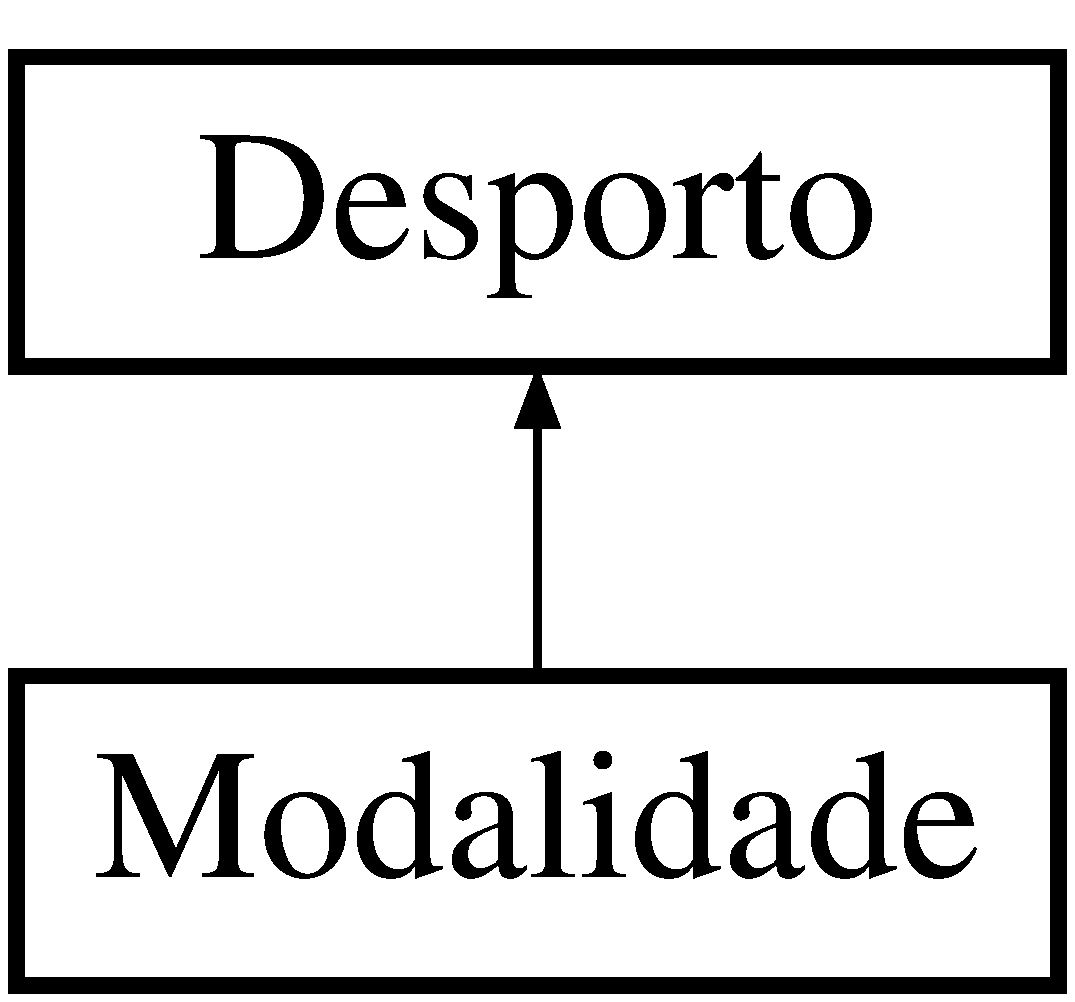
\includegraphics[height=2.000000cm]{class_desporto}
\end{center}
\end{figure}
\subsection*{Public Member Functions}
\begin{DoxyCompactItemize}
\item 
\hyperlink{class_desporto_af6abc41a2b8a416e475afb9409226ef6}{Desporto} ()
\item 
\hyperlink{class_desporto_adeb528d743b915077851def7c5ca61c2}{Desporto} (string n)
\item 
virtual \hyperlink{class_desporto_a7b6a35a34e1b599f7531d1af92c35557}{$\sim$\+Desporto} ()
\item 
virtual void \hyperlink{class_desporto_ac5babc7f79c7765c48a1ebe8ea9ba3b4}{set\+Nome} (string n)
\item 
virtual unsigned int \hyperlink{class_desporto_ab03f722e71568b7235c9499876f849c6}{get\+N\+Jogadores} () const  =0
\item 
virtual string \hyperlink{class_desporto_ac55230ea2713d66a7e1c3e8731a4b601}{get\+Nome} () const 
\item 
virtual void \hyperlink{class_desporto_a8f2b72b4e8446f36cbb59caab28e22ff}{calc\+Pont} ()
\end{DoxyCompactItemize}
\subsection*{Private Attributes}
\begin{DoxyCompactItemize}
\item 
string \hyperlink{class_desporto_ad7ccd705ac44cd574cbe1290a698d040}{nome}
\end{DoxyCompactItemize}


\subsection{Constructor \& Destructor Documentation}
\hypertarget{class_desporto_af6abc41a2b8a416e475afb9409226ef6}{}\index{Desporto@{Desporto}!Desporto@{Desporto}}
\index{Desporto@{Desporto}!Desporto@{Desporto}}
\subsubsection[{Desporto()}]{\setlength{\rightskip}{0pt plus 5cm}Desporto\+::\+Desporto (
\begin{DoxyParamCaption}
{}
\end{DoxyParamCaption}
)\hspace{0.3cm}{\ttfamily [inline]}}\label{class_desporto_af6abc41a2b8a416e475afb9409226ef6}
\hypertarget{class_desporto_adeb528d743b915077851def7c5ca61c2}{}\index{Desporto@{Desporto}!Desporto@{Desporto}}
\index{Desporto@{Desporto}!Desporto@{Desporto}}
\subsubsection[{Desporto(string n)}]{\setlength{\rightskip}{0pt plus 5cm}Desporto\+::\+Desporto (
\begin{DoxyParamCaption}
\item[{string}]{n}
\end{DoxyParamCaption}
)\hspace{0.3cm}{\ttfamily [inline]}}\label{class_desporto_adeb528d743b915077851def7c5ca61c2}
\hypertarget{class_desporto_a7b6a35a34e1b599f7531d1af92c35557}{}\index{Desporto@{Desporto}!````~Desporto@{$\sim$\+Desporto}}
\index{````~Desporto@{$\sim$\+Desporto}!Desporto@{Desporto}}
\subsubsection[{$\sim$\+Desporto()}]{\setlength{\rightskip}{0pt plus 5cm}virtual Desporto\+::$\sim$\+Desporto (
\begin{DoxyParamCaption}
{}
\end{DoxyParamCaption}
)\hspace{0.3cm}{\ttfamily [inline]}, {\ttfamily [virtual]}}\label{class_desporto_a7b6a35a34e1b599f7531d1af92c35557}


\subsection{Member Function Documentation}
\hypertarget{class_desporto_a8f2b72b4e8446f36cbb59caab28e22ff}{}\index{Desporto@{Desporto}!calc\+Pont@{calc\+Pont}}
\index{calc\+Pont@{calc\+Pont}!Desporto@{Desporto}}
\subsubsection[{calc\+Pont()}]{\setlength{\rightskip}{0pt plus 5cm}virtual void Desporto\+::calc\+Pont (
\begin{DoxyParamCaption}
{}
\end{DoxyParamCaption}
)\hspace{0.3cm}{\ttfamily [inline]}, {\ttfamily [virtual]}}\label{class_desporto_a8f2b72b4e8446f36cbb59caab28e22ff}
\hypertarget{class_desporto_ab03f722e71568b7235c9499876f849c6}{}\index{Desporto@{Desporto}!get\+N\+Jogadores@{get\+N\+Jogadores}}
\index{get\+N\+Jogadores@{get\+N\+Jogadores}!Desporto@{Desporto}}
\subsubsection[{get\+N\+Jogadores() const  =0}]{\setlength{\rightskip}{0pt plus 5cm}virtual unsigned int Desporto\+::get\+N\+Jogadores (
\begin{DoxyParamCaption}
{}
\end{DoxyParamCaption}
) const\hspace{0.3cm}{\ttfamily [pure virtual]}}\label{class_desporto_ab03f722e71568b7235c9499876f849c6}


Implemented in \hyperlink{class_modalidade_ae9016743d83bb1bd83ae1c076db5e65c}{Modalidade}.

\hypertarget{class_desporto_ac55230ea2713d66a7e1c3e8731a4b601}{}\index{Desporto@{Desporto}!get\+Nome@{get\+Nome}}
\index{get\+Nome@{get\+Nome}!Desporto@{Desporto}}
\subsubsection[{get\+Nome() const }]{\setlength{\rightskip}{0pt plus 5cm}virtual string Desporto\+::get\+Nome (
\begin{DoxyParamCaption}
{}
\end{DoxyParamCaption}
) const\hspace{0.3cm}{\ttfamily [inline]}, {\ttfamily [virtual]}}\label{class_desporto_ac55230ea2713d66a7e1c3e8731a4b601}


Reimplemented in \hyperlink{class_modalidade_a46003f6a0dceac894f92971a6df9e4a7}{Modalidade}.

\hypertarget{class_desporto_ac5babc7f79c7765c48a1ebe8ea9ba3b4}{}\index{Desporto@{Desporto}!set\+Nome@{set\+Nome}}
\index{set\+Nome@{set\+Nome}!Desporto@{Desporto}}
\subsubsection[{set\+Nome(string n)}]{\setlength{\rightskip}{0pt plus 5cm}virtual void Desporto\+::set\+Nome (
\begin{DoxyParamCaption}
\item[{string}]{n}
\end{DoxyParamCaption}
)\hspace{0.3cm}{\ttfamily [inline]}, {\ttfamily [virtual]}}\label{class_desporto_ac5babc7f79c7765c48a1ebe8ea9ba3b4}


\subsection{Member Data Documentation}
\hypertarget{class_desporto_ad7ccd705ac44cd574cbe1290a698d040}{}\index{Desporto@{Desporto}!nome@{nome}}
\index{nome@{nome}!Desporto@{Desporto}}
\subsubsection[{nome}]{\setlength{\rightskip}{0pt plus 5cm}string Desporto\+::nome\hspace{0.3cm}{\ttfamily [private]}}\label{class_desporto_ad7ccd705ac44cd574cbe1290a698d040}


The documentation for this class was generated from the following file\+:\begin{DoxyCompactItemize}
\item 
C\+:/\+Users/\+Alexandre/\+Git\+Hub/\+A\+E\+D\+A\+\_\+\+P\+R\+O\+J\+E\+C\+T\+O\+\_\+1/src/logic/\hyperlink{_desporto_8h}{Desporto.\+h}\end{DoxyCompactItemize}

\hypertarget{structeq_bilhete}{}\section{eq\+Bilhete Struct Reference}
\label{structeq_bilhete}\index{eq\+Bilhete@{eq\+Bilhete}}


{\ttfamily \#include $<$Campeonato.\+h$>$}

\subsection*{Public Member Functions}
\begin{DoxyCompactItemize}
\item 
bool \hyperlink{structeq_bilhete_a28de41742af6d1f7db86514d012dc979}{operator()} (const \hyperlink{class_bilhete}{Bilhete} \&b1, const \hyperlink{class_bilhete}{Bilhete} \&b2) const 
\end{DoxyCompactItemize}


\subsection{Member Function Documentation}
\hypertarget{structeq_bilhete_a28de41742af6d1f7db86514d012dc979}{}\index{eq\+Bilhete@{eq\+Bilhete}!operator()@{operator()}}
\index{operator()@{operator()}!eq\+Bilhete@{eq\+Bilhete}}
\subsubsection[{operator()(const Bilhete \&b1, const Bilhete \&b2) const }]{\setlength{\rightskip}{0pt plus 5cm}bool eq\+Bilhete\+::operator() (
\begin{DoxyParamCaption}
\item[{const {\bf Bilhete} \&}]{b1, }
\item[{const {\bf Bilhete} \&}]{b2}
\end{DoxyParamCaption}
) const\hspace{0.3cm}{\ttfamily [inline]}}\label{structeq_bilhete_a28de41742af6d1f7db86514d012dc979}


The documentation for this struct was generated from the following file\+:\begin{DoxyCompactItemize}
\item 
C\+:/\+Users/\+Alexandre/\+Git\+Hub/\+A\+E\+D\+A\+\_\+\+P\+R\+O\+J\+E\+C\+T\+O\+\_\+1/src/logic/\hyperlink{_campeonato_8h}{Campeonato.\+h}\end{DoxyCompactItemize}

\hypertarget{class_equipa}{}\section{Equipa Class Reference}
\label{class_equipa}\index{Equipa@{Equipa}}


{\ttfamily \#include $<$Equipa.\+h$>$}

\subsection*{Public Member Functions}
\begin{DoxyCompactItemize}
\item 
\hyperlink{class_equipa_a2721072fa0d6b4451d22fdfe3c3f3c0e}{Equipa} (string n, string p, string pat)
\item 
\hyperlink{class_equipa_a71e864835165c2be093784ef38fd634d}{Equipa} ()
\item 
string \hyperlink{class_equipa_a9d20d0c8daa94e7562c5ea173337a224}{get\+Nome} () const 
\item 
void \hyperlink{class_equipa_a13e90216eb9ca9d6b2c144295a2b6730}{set\+Nome} (string novo\+Nome)
\item 
string \hyperlink{class_equipa_ac0d2108875ef6ed5833bfbd2f9921625}{get\+Pais} () const 
\item 
void \hyperlink{class_equipa_a2360f13c75fdcf75395cef84a9d0f589}{set\+Pais} (string novo\+Pais)
\item 
string \hyperlink{class_equipa_a241ab40d7dfe77af53b834482c79b94f}{get\+Patrocinador} () const 
\item 
void \hyperlink{class_equipa_aca1891ba657401bff00291ab22bb430a}{set\+Patrocinador} (string novo\+Patrocinio)
\item 
float \hyperlink{class_equipa_aeccebdc0af7faf1553e7c7eefe9e66af}{get\+Pontuacao} () const 
\item 
void \hyperlink{class_equipa_a9b63be5bd83117f9bd71bfa6e140da0d}{set\+Pontuacao} (float p)
\item 
vector$<$ \hyperlink{class_atleta}{Atleta} $\ast$ $>$ \hyperlink{class_equipa_a24c4de83cc1171ce42f442ef7be8a7c4}{get\+Atletas} () const 
\item 
\hyperlink{class_atleta}{Atleta} $\ast$ \hyperlink{class_equipa_a9b3eaddbfd2944cffb37f242cba00fa1}{get\+Atleta} (unsigned int id)
\item 
void \hyperlink{class_equipa_a67f982e822a7772f2668301db0e147eb}{inserir\+Atleta} (\hyperlink{class_atleta}{Atleta} \&a1)
\item 
bool \hyperlink{class_equipa_a12d4f1b639138a62482483e730f1c85f}{eliminar\+Atleta} (unsigned int id)
\item 
int \hyperlink{class_equipa_a9ad2d95727dfd39cf788e5c5a49b03d9}{existe\+Atleta} (string \hyperlink{class_equipa_a8373ab9d0fe95ae0c231bf2d9707e759}{nome})
\item 
int \hyperlink{class_equipa_ade9df7fbce5c76b859cb15331f7d38b9}{existe\+Atleta\+I\+D} (unsigned int id)
\item 
void \hyperlink{class_equipa_ab17ae44fbe5b5dd2d7eea4a6d752f518}{show\+Atletas} ()
\item 
void \hyperlink{class_equipa_a1329201fd3f78cf3b7c9c146578af92f}{imprime} ()
\item 
bool \hyperlink{class_equipa_a74c301834fdd69406680d35ec0abdca6}{operator$<$} (const \hyperlink{class_equipa}{Equipa} \&e)
\end{DoxyCompactItemize}
\subsection*{Private Attributes}
\begin{DoxyCompactItemize}
\item 
string \hyperlink{class_equipa_a8373ab9d0fe95ae0c231bf2d9707e759}{nome}
\item 
string \hyperlink{class_equipa_a9972aebf308a7adcd5e23d127639311f}{pais}
\item 
string \hyperlink{class_equipa_ac9a1c45750e118888d61930c3bf4d185}{patrocinador}
\item 
float \hyperlink{class_equipa_a1b047e8ef3d73dd54b656af9dbfcf9ae}{pontuacao}
\item 
vector$<$ \hyperlink{class_atleta}{Atleta} $\ast$ $>$ \hyperlink{class_equipa_a391f6bca285bedd992f0104a17b79719}{atletas}
\end{DoxyCompactItemize}


\subsection{Constructor \& Destructor Documentation}
\hypertarget{class_equipa_a2721072fa0d6b4451d22fdfe3c3f3c0e}{}\index{Equipa@{Equipa}!Equipa@{Equipa}}
\index{Equipa@{Equipa}!Equipa@{Equipa}}
\subsubsection[{Equipa(string n, string p, string pat)}]{\setlength{\rightskip}{0pt plus 5cm}Equipa\+::\+Equipa (
\begin{DoxyParamCaption}
\item[{string}]{n, }
\item[{string}]{p, }
\item[{string}]{pat}
\end{DoxyParamCaption}
)}\label{class_equipa_a2721072fa0d6b4451d22fdfe3c3f3c0e}
\hypertarget{class_equipa_a71e864835165c2be093784ef38fd634d}{}\index{Equipa@{Equipa}!Equipa@{Equipa}}
\index{Equipa@{Equipa}!Equipa@{Equipa}}
\subsubsection[{Equipa()}]{\setlength{\rightskip}{0pt plus 5cm}Equipa\+::\+Equipa (
\begin{DoxyParamCaption}
{}
\end{DoxyParamCaption}
)}\label{class_equipa_a71e864835165c2be093784ef38fd634d}


\subsection{Member Function Documentation}
\hypertarget{class_equipa_a12d4f1b639138a62482483e730f1c85f}{}\index{Equipa@{Equipa}!eliminar\+Atleta@{eliminar\+Atleta}}
\index{eliminar\+Atleta@{eliminar\+Atleta}!Equipa@{Equipa}}
\subsubsection[{eliminar\+Atleta(unsigned int id)}]{\setlength{\rightskip}{0pt plus 5cm}bool Equipa\+::eliminar\+Atleta (
\begin{DoxyParamCaption}
\item[{unsigned int}]{id}
\end{DoxyParamCaption}
)}\label{class_equipa_a12d4f1b639138a62482483e730f1c85f}
\hypertarget{class_equipa_a9ad2d95727dfd39cf788e5c5a49b03d9}{}\index{Equipa@{Equipa}!existe\+Atleta@{existe\+Atleta}}
\index{existe\+Atleta@{existe\+Atleta}!Equipa@{Equipa}}
\subsubsection[{existe\+Atleta(string nome)}]{\setlength{\rightskip}{0pt plus 5cm}int Equipa\+::existe\+Atleta (
\begin{DoxyParamCaption}
\item[{string}]{nome}
\end{DoxyParamCaption}
)}\label{class_equipa_a9ad2d95727dfd39cf788e5c5a49b03d9}
\hypertarget{class_equipa_ade9df7fbce5c76b859cb15331f7d38b9}{}\index{Equipa@{Equipa}!existe\+Atleta\+I\+D@{existe\+Atleta\+I\+D}}
\index{existe\+Atleta\+I\+D@{existe\+Atleta\+I\+D}!Equipa@{Equipa}}
\subsubsection[{existe\+Atleta\+I\+D(unsigned int id)}]{\setlength{\rightskip}{0pt plus 5cm}int Equipa\+::existe\+Atleta\+I\+D (
\begin{DoxyParamCaption}
\item[{unsigned int}]{id}
\end{DoxyParamCaption}
)}\label{class_equipa_ade9df7fbce5c76b859cb15331f7d38b9}
\hypertarget{class_equipa_a9b3eaddbfd2944cffb37f242cba00fa1}{}\index{Equipa@{Equipa}!get\+Atleta@{get\+Atleta}}
\index{get\+Atleta@{get\+Atleta}!Equipa@{Equipa}}
\subsubsection[{get\+Atleta(unsigned int id)}]{\setlength{\rightskip}{0pt plus 5cm}{\bf Atleta} $\ast$ Equipa\+::get\+Atleta (
\begin{DoxyParamCaption}
\item[{unsigned int}]{id}
\end{DoxyParamCaption}
)}\label{class_equipa_a9b3eaddbfd2944cffb37f242cba00fa1}
\hypertarget{class_equipa_a24c4de83cc1171ce42f442ef7be8a7c4}{}\index{Equipa@{Equipa}!get\+Atletas@{get\+Atletas}}
\index{get\+Atletas@{get\+Atletas}!Equipa@{Equipa}}
\subsubsection[{get\+Atletas() const }]{\setlength{\rightskip}{0pt plus 5cm}vector$<$ {\bf Atleta} $\ast$ $>$ Equipa\+::get\+Atletas (
\begin{DoxyParamCaption}
{}
\end{DoxyParamCaption}
) const}\label{class_equipa_a24c4de83cc1171ce42f442ef7be8a7c4}
\hypertarget{class_equipa_a9d20d0c8daa94e7562c5ea173337a224}{}\index{Equipa@{Equipa}!get\+Nome@{get\+Nome}}
\index{get\+Nome@{get\+Nome}!Equipa@{Equipa}}
\subsubsection[{get\+Nome() const }]{\setlength{\rightskip}{0pt plus 5cm}string Equipa\+::get\+Nome (
\begin{DoxyParamCaption}
{}
\end{DoxyParamCaption}
) const}\label{class_equipa_a9d20d0c8daa94e7562c5ea173337a224}
\hypertarget{class_equipa_ac0d2108875ef6ed5833bfbd2f9921625}{}\index{Equipa@{Equipa}!get\+Pais@{get\+Pais}}
\index{get\+Pais@{get\+Pais}!Equipa@{Equipa}}
\subsubsection[{get\+Pais() const }]{\setlength{\rightskip}{0pt plus 5cm}string Equipa\+::get\+Pais (
\begin{DoxyParamCaption}
{}
\end{DoxyParamCaption}
) const}\label{class_equipa_ac0d2108875ef6ed5833bfbd2f9921625}
\hypertarget{class_equipa_a241ab40d7dfe77af53b834482c79b94f}{}\index{Equipa@{Equipa}!get\+Patrocinador@{get\+Patrocinador}}
\index{get\+Patrocinador@{get\+Patrocinador}!Equipa@{Equipa}}
\subsubsection[{get\+Patrocinador() const }]{\setlength{\rightskip}{0pt plus 5cm}string Equipa\+::get\+Patrocinador (
\begin{DoxyParamCaption}
{}
\end{DoxyParamCaption}
) const}\label{class_equipa_a241ab40d7dfe77af53b834482c79b94f}
\hypertarget{class_equipa_aeccebdc0af7faf1553e7c7eefe9e66af}{}\index{Equipa@{Equipa}!get\+Pontuacao@{get\+Pontuacao}}
\index{get\+Pontuacao@{get\+Pontuacao}!Equipa@{Equipa}}
\subsubsection[{get\+Pontuacao() const }]{\setlength{\rightskip}{0pt plus 5cm}float Equipa\+::get\+Pontuacao (
\begin{DoxyParamCaption}
{}
\end{DoxyParamCaption}
) const}\label{class_equipa_aeccebdc0af7faf1553e7c7eefe9e66af}
\hypertarget{class_equipa_a1329201fd3f78cf3b7c9c146578af92f}{}\index{Equipa@{Equipa}!imprime@{imprime}}
\index{imprime@{imprime}!Equipa@{Equipa}}
\subsubsection[{imprime()}]{\setlength{\rightskip}{0pt plus 5cm}void Equipa\+::imprime (
\begin{DoxyParamCaption}
{}
\end{DoxyParamCaption}
)}\label{class_equipa_a1329201fd3f78cf3b7c9c146578af92f}
\hypertarget{class_equipa_a67f982e822a7772f2668301db0e147eb}{}\index{Equipa@{Equipa}!inserir\+Atleta@{inserir\+Atleta}}
\index{inserir\+Atleta@{inserir\+Atleta}!Equipa@{Equipa}}
\subsubsection[{inserir\+Atleta(\+Atleta \&a1)}]{\setlength{\rightskip}{0pt plus 5cm}void Equipa\+::inserir\+Atleta (
\begin{DoxyParamCaption}
\item[{{\bf Atleta} \&}]{a1}
\end{DoxyParamCaption}
)}\label{class_equipa_a67f982e822a7772f2668301db0e147eb}
\hypertarget{class_equipa_a74c301834fdd69406680d35ec0abdca6}{}\index{Equipa@{Equipa}!operator$<$@{operator$<$}}
\index{operator$<$@{operator$<$}!Equipa@{Equipa}}
\subsubsection[{operator$<$(const Equipa \&e)}]{\setlength{\rightskip}{0pt plus 5cm}bool Equipa\+::operator$<$ (
\begin{DoxyParamCaption}
\item[{const {\bf Equipa} \&}]{e}
\end{DoxyParamCaption}
)}\label{class_equipa_a74c301834fdd69406680d35ec0abdca6}
\hypertarget{class_equipa_a13e90216eb9ca9d6b2c144295a2b6730}{}\index{Equipa@{Equipa}!set\+Nome@{set\+Nome}}
\index{set\+Nome@{set\+Nome}!Equipa@{Equipa}}
\subsubsection[{set\+Nome(string novo\+Nome)}]{\setlength{\rightskip}{0pt plus 5cm}void Equipa\+::set\+Nome (
\begin{DoxyParamCaption}
\item[{string}]{novo\+Nome}
\end{DoxyParamCaption}
)}\label{class_equipa_a13e90216eb9ca9d6b2c144295a2b6730}
\hypertarget{class_equipa_a2360f13c75fdcf75395cef84a9d0f589}{}\index{Equipa@{Equipa}!set\+Pais@{set\+Pais}}
\index{set\+Pais@{set\+Pais}!Equipa@{Equipa}}
\subsubsection[{set\+Pais(string novo\+Pais)}]{\setlength{\rightskip}{0pt plus 5cm}void Equipa\+::set\+Pais (
\begin{DoxyParamCaption}
\item[{string}]{novo\+Pais}
\end{DoxyParamCaption}
)}\label{class_equipa_a2360f13c75fdcf75395cef84a9d0f589}
\hypertarget{class_equipa_aca1891ba657401bff00291ab22bb430a}{}\index{Equipa@{Equipa}!set\+Patrocinador@{set\+Patrocinador}}
\index{set\+Patrocinador@{set\+Patrocinador}!Equipa@{Equipa}}
\subsubsection[{set\+Patrocinador(string novo\+Patrocinio)}]{\setlength{\rightskip}{0pt plus 5cm}void Equipa\+::set\+Patrocinador (
\begin{DoxyParamCaption}
\item[{string}]{novo\+Patrocinio}
\end{DoxyParamCaption}
)}\label{class_equipa_aca1891ba657401bff00291ab22bb430a}
\hypertarget{class_equipa_a9b63be5bd83117f9bd71bfa6e140da0d}{}\index{Equipa@{Equipa}!set\+Pontuacao@{set\+Pontuacao}}
\index{set\+Pontuacao@{set\+Pontuacao}!Equipa@{Equipa}}
\subsubsection[{set\+Pontuacao(float p)}]{\setlength{\rightskip}{0pt plus 5cm}void Equipa\+::set\+Pontuacao (
\begin{DoxyParamCaption}
\item[{float}]{p}
\end{DoxyParamCaption}
)}\label{class_equipa_a9b63be5bd83117f9bd71bfa6e140da0d}
\hypertarget{class_equipa_ab17ae44fbe5b5dd2d7eea4a6d752f518}{}\index{Equipa@{Equipa}!show\+Atletas@{show\+Atletas}}
\index{show\+Atletas@{show\+Atletas}!Equipa@{Equipa}}
\subsubsection[{show\+Atletas()}]{\setlength{\rightskip}{0pt plus 5cm}void Equipa\+::show\+Atletas (
\begin{DoxyParamCaption}
{}
\end{DoxyParamCaption}
)}\label{class_equipa_ab17ae44fbe5b5dd2d7eea4a6d752f518}


\subsection{Member Data Documentation}
\hypertarget{class_equipa_a391f6bca285bedd992f0104a17b79719}{}\index{Equipa@{Equipa}!atletas@{atletas}}
\index{atletas@{atletas}!Equipa@{Equipa}}
\subsubsection[{atletas}]{\setlength{\rightskip}{0pt plus 5cm}vector$<${\bf Atleta}$\ast$$>$ Equipa\+::atletas\hspace{0.3cm}{\ttfamily [private]}}\label{class_equipa_a391f6bca285bedd992f0104a17b79719}
\hypertarget{class_equipa_a8373ab9d0fe95ae0c231bf2d9707e759}{}\index{Equipa@{Equipa}!nome@{nome}}
\index{nome@{nome}!Equipa@{Equipa}}
\subsubsection[{nome}]{\setlength{\rightskip}{0pt plus 5cm}string Equipa\+::nome\hspace{0.3cm}{\ttfamily [private]}}\label{class_equipa_a8373ab9d0fe95ae0c231bf2d9707e759}
\hypertarget{class_equipa_a9972aebf308a7adcd5e23d127639311f}{}\index{Equipa@{Equipa}!pais@{pais}}
\index{pais@{pais}!Equipa@{Equipa}}
\subsubsection[{pais}]{\setlength{\rightskip}{0pt plus 5cm}string Equipa\+::pais\hspace{0.3cm}{\ttfamily [private]}}\label{class_equipa_a9972aebf308a7adcd5e23d127639311f}
\hypertarget{class_equipa_ac9a1c45750e118888d61930c3bf4d185}{}\index{Equipa@{Equipa}!patrocinador@{patrocinador}}
\index{patrocinador@{patrocinador}!Equipa@{Equipa}}
\subsubsection[{patrocinador}]{\setlength{\rightskip}{0pt plus 5cm}string Equipa\+::patrocinador\hspace{0.3cm}{\ttfamily [private]}}\label{class_equipa_ac9a1c45750e118888d61930c3bf4d185}
\hypertarget{class_equipa_a1b047e8ef3d73dd54b656af9dbfcf9ae}{}\index{Equipa@{Equipa}!pontuacao@{pontuacao}}
\index{pontuacao@{pontuacao}!Equipa@{Equipa}}
\subsubsection[{pontuacao}]{\setlength{\rightskip}{0pt plus 5cm}float Equipa\+::pontuacao\hspace{0.3cm}{\ttfamily [private]}}\label{class_equipa_a1b047e8ef3d73dd54b656af9dbfcf9ae}


The documentation for this class was generated from the following files\+:\begin{DoxyCompactItemize}
\item 
C\+:/\+Users/\+Alexandre/\+Git\+Hub/\+A\+E\+D\+A\+\_\+\+P\+R\+O\+J\+E\+C\+T\+O\+\_\+1/src/logic/\hyperlink{_equipa_8h}{Equipa.\+h}\item 
C\+:/\+Users/\+Alexandre/\+Git\+Hub/\+A\+E\+D\+A\+\_\+\+P\+R\+O\+J\+E\+C\+T\+O\+\_\+1/src/logic/\hyperlink{_equipa_8cpp}{Equipa.\+cpp}\end{DoxyCompactItemize}

\hypertarget{class_equipa_inexistente}{}\section{Equipa\+Inexistente Class Reference}
\label{class_equipa_inexistente}\index{Equipa\+Inexistente@{Equipa\+Inexistente}}


{\ttfamily \#include $<$Utilities.\+h$>$}

\subsection*{Public Member Functions}
\begin{DoxyCompactItemize}
\item 
\hyperlink{class_equipa_inexistente_a9e501ec33356ba0deeebcc4679846939}{Equipa\+Inexistente} (string n)
\item 
string \hyperlink{class_equipa_inexistente_a4660d6c1839f46d3666a092c1af2cb7c}{get\+Nome} ()
\end{DoxyCompactItemize}
\subsection*{Public Attributes}
\begin{DoxyCompactItemize}
\item 
string \hyperlink{class_equipa_inexistente_a75deb0b7ca08921ff1f9e9cc558609d0}{nome}
\end{DoxyCompactItemize}


\subsection{Constructor \& Destructor Documentation}
\hypertarget{class_equipa_inexistente_a9e501ec33356ba0deeebcc4679846939}{}\index{Equipa\+Inexistente@{Equipa\+Inexistente}!Equipa\+Inexistente@{Equipa\+Inexistente}}
\index{Equipa\+Inexistente@{Equipa\+Inexistente}!Equipa\+Inexistente@{Equipa\+Inexistente}}
\subsubsection[{Equipa\+Inexistente(string n)}]{\setlength{\rightskip}{0pt plus 5cm}Equipa\+Inexistente\+::\+Equipa\+Inexistente (
\begin{DoxyParamCaption}
\item[{string}]{n}
\end{DoxyParamCaption}
)\hspace{0.3cm}{\ttfamily [inline]}}\label{class_equipa_inexistente_a9e501ec33356ba0deeebcc4679846939}


\subsection{Member Function Documentation}
\hypertarget{class_equipa_inexistente_a4660d6c1839f46d3666a092c1af2cb7c}{}\index{Equipa\+Inexistente@{Equipa\+Inexistente}!get\+Nome@{get\+Nome}}
\index{get\+Nome@{get\+Nome}!Equipa\+Inexistente@{Equipa\+Inexistente}}
\subsubsection[{get\+Nome()}]{\setlength{\rightskip}{0pt plus 5cm}string Equipa\+Inexistente\+::get\+Nome (
\begin{DoxyParamCaption}
{}
\end{DoxyParamCaption}
)\hspace{0.3cm}{\ttfamily [inline]}}\label{class_equipa_inexistente_a4660d6c1839f46d3666a092c1af2cb7c}


\subsection{Member Data Documentation}
\hypertarget{class_equipa_inexistente_a75deb0b7ca08921ff1f9e9cc558609d0}{}\index{Equipa\+Inexistente@{Equipa\+Inexistente}!nome@{nome}}
\index{nome@{nome}!Equipa\+Inexistente@{Equipa\+Inexistente}}
\subsubsection[{nome}]{\setlength{\rightskip}{0pt plus 5cm}string Equipa\+Inexistente\+::nome}\label{class_equipa_inexistente_a75deb0b7ca08921ff1f9e9cc558609d0}


The documentation for this class was generated from the following file\+:\begin{DoxyCompactItemize}
\item 
C\+:/\+Users/\+Alexandre/\+Git\+Hub/\+A\+E\+D\+A\+\_\+\+P\+R\+O\+J\+E\+C\+T\+O\+\_\+1/src/logic/\hyperlink{_utilities_8h}{Utilities.\+h}\end{DoxyCompactItemize}

\hypertarget{class_erro_no_ficheiro}{}\section{Erro\+No\+Ficheiro Class Reference}
\label{class_erro_no_ficheiro}\index{Erro\+No\+Ficheiro@{Erro\+No\+Ficheiro}}


{\ttfamily \#include $<$Utilities.\+h$>$}

\subsection*{Public Member Functions}
\begin{DoxyCompactItemize}
\item 
\hyperlink{class_erro_no_ficheiro_a23932fdaf17051c64d9131b92ee9876d}{Erro\+No\+Ficheiro} (string fn)
\item 
string \hyperlink{class_erro_no_ficheiro_aab06f74cf69c355b122ad19676f08ec1}{get\+File\+Name} ()
\end{DoxyCompactItemize}
\subsection*{Public Attributes}
\begin{DoxyCompactItemize}
\item 
string \hyperlink{class_erro_no_ficheiro_a2e7b7c6fce4c5633ddef2c4a7d3cca0d}{filename}
\end{DoxyCompactItemize}


\subsection{Constructor \& Destructor Documentation}
\hypertarget{class_erro_no_ficheiro_a23932fdaf17051c64d9131b92ee9876d}{}\index{Erro\+No\+Ficheiro@{Erro\+No\+Ficheiro}!Erro\+No\+Ficheiro@{Erro\+No\+Ficheiro}}
\index{Erro\+No\+Ficheiro@{Erro\+No\+Ficheiro}!Erro\+No\+Ficheiro@{Erro\+No\+Ficheiro}}
\subsubsection[{Erro\+No\+Ficheiro(string fn)}]{\setlength{\rightskip}{0pt plus 5cm}Erro\+No\+Ficheiro\+::\+Erro\+No\+Ficheiro (
\begin{DoxyParamCaption}
\item[{string}]{fn}
\end{DoxyParamCaption}
)\hspace{0.3cm}{\ttfamily [inline]}}\label{class_erro_no_ficheiro_a23932fdaf17051c64d9131b92ee9876d}


\subsection{Member Function Documentation}
\hypertarget{class_erro_no_ficheiro_aab06f74cf69c355b122ad19676f08ec1}{}\index{Erro\+No\+Ficheiro@{Erro\+No\+Ficheiro}!get\+File\+Name@{get\+File\+Name}}
\index{get\+File\+Name@{get\+File\+Name}!Erro\+No\+Ficheiro@{Erro\+No\+Ficheiro}}
\subsubsection[{get\+File\+Name()}]{\setlength{\rightskip}{0pt plus 5cm}string Erro\+No\+Ficheiro\+::get\+File\+Name (
\begin{DoxyParamCaption}
{}
\end{DoxyParamCaption}
)\hspace{0.3cm}{\ttfamily [inline]}}\label{class_erro_no_ficheiro_aab06f74cf69c355b122ad19676f08ec1}


\subsection{Member Data Documentation}
\hypertarget{class_erro_no_ficheiro_a2e7b7c6fce4c5633ddef2c4a7d3cca0d}{}\index{Erro\+No\+Ficheiro@{Erro\+No\+Ficheiro}!filename@{filename}}
\index{filename@{filename}!Erro\+No\+Ficheiro@{Erro\+No\+Ficheiro}}
\subsubsection[{filename}]{\setlength{\rightskip}{0pt plus 5cm}string Erro\+No\+Ficheiro\+::filename}\label{class_erro_no_ficheiro_a2e7b7c6fce4c5633ddef2c4a7d3cca0d}


The documentation for this class was generated from the following file\+:\begin{DoxyCompactItemize}
\item 
C\+:/\+Users/\+Alexandre/\+Git\+Hub/\+A\+E\+D\+A\+\_\+\+P\+R\+O\+J\+E\+C\+T\+O\+\_\+1/src/logic/\hyperlink{_utilities_8h}{Utilities.\+h}\end{DoxyCompactItemize}

\hypertarget{class_atletas_guardados_1_1_erro_no_ficheiro}{}\section{Atletas\+Guardados\+:\+:Erro\+No\+Ficheiro Class Reference}
\label{class_atletas_guardados_1_1_erro_no_ficheiro}\index{Atletas\+Guardados\+::\+Erro\+No\+Ficheiro@{Atletas\+Guardados\+::\+Erro\+No\+Ficheiro}}


{\ttfamily \#include $<$Atleta.\+h$>$}

\subsection*{Public Member Functions}
\begin{DoxyCompactItemize}
\item 
\hyperlink{class_atletas_guardados_1_1_erro_no_ficheiro_ad9c18a84af81a0e430e2244fba89c828}{Erro\+No\+Ficheiro} ()
\end{DoxyCompactItemize}


\subsection{Constructor \& Destructor Documentation}
\hypertarget{class_atletas_guardados_1_1_erro_no_ficheiro_ad9c18a84af81a0e430e2244fba89c828}{}\index{Atletas\+Guardados\+::\+Erro\+No\+Ficheiro@{Atletas\+Guardados\+::\+Erro\+No\+Ficheiro}!Erro\+No\+Ficheiro@{Erro\+No\+Ficheiro}}
\index{Erro\+No\+Ficheiro@{Erro\+No\+Ficheiro}!Atletas\+Guardados\+::\+Erro\+No\+Ficheiro@{Atletas\+Guardados\+::\+Erro\+No\+Ficheiro}}
\subsubsection[{Erro\+No\+Ficheiro()}]{\setlength{\rightskip}{0pt plus 5cm}Atletas\+Guardados\+::\+Erro\+No\+Ficheiro\+::\+Erro\+No\+Ficheiro (
\begin{DoxyParamCaption}
{}
\end{DoxyParamCaption}
)\hspace{0.3cm}{\ttfamily [inline]}}\label{class_atletas_guardados_1_1_erro_no_ficheiro_ad9c18a84af81a0e430e2244fba89c828}


The documentation for this class was generated from the following file\+:\begin{DoxyCompactItemize}
\item 
C\+:/\+Users/\+Alexandre/\+Git\+Hub/\+A\+E\+D\+A\+\_\+\+P\+R\+O\+J\+E\+C\+T\+O\+\_\+1/src/logic/\hyperlink{_atleta_8h}{Atleta.\+h}\end{DoxyCompactItemize}

\hypertarget{structhash__atletas}{}\section{hash\+\_\+atletas Struct Reference}
\label{structhash__atletas}\index{hash\+\_\+atletas@{hash\+\_\+atletas}}


{\ttfamily \#include $<$Atleta.\+h$>$}

\subsection*{Public Member Functions}
\begin{DoxyCompactItemize}
\item 
int \hyperlink{structhash__atletas_a587486cb48f2cbdab96d48dea441efb0}{operator()} (const \hyperlink{class_atleta}{Atleta} \&a1) const 
\item 
bool \hyperlink{structhash__atletas_ac7f1ef34cb53777e99323c8bf58cde02}{operator()} (const \hyperlink{class_atleta}{Atleta} \&a1, const \hyperlink{class_atleta}{Atleta} \&a2) const 
\end{DoxyCompactItemize}


\subsection{Member Function Documentation}
\hypertarget{structhash__atletas_a587486cb48f2cbdab96d48dea441efb0}{}\index{hash\+\_\+atletas@{hash\+\_\+atletas}!operator()@{operator()}}
\index{operator()@{operator()}!hash\+\_\+atletas@{hash\+\_\+atletas}}
\subsubsection[{operator()(const Atleta \&a1) const }]{\setlength{\rightskip}{0pt plus 5cm}int hash\+\_\+atletas\+::operator() (
\begin{DoxyParamCaption}
\item[{const {\bf Atleta} \&}]{a1}
\end{DoxyParamCaption}
) const\hspace{0.3cm}{\ttfamily [inline]}}\label{structhash__atletas_a587486cb48f2cbdab96d48dea441efb0}
\hypertarget{structhash__atletas_ac7f1ef34cb53777e99323c8bf58cde02}{}\index{hash\+\_\+atletas@{hash\+\_\+atletas}!operator()@{operator()}}
\index{operator()@{operator()}!hash\+\_\+atletas@{hash\+\_\+atletas}}
\subsubsection[{operator()(const Atleta \&a1, const Atleta \&a2) const }]{\setlength{\rightskip}{0pt plus 5cm}bool hash\+\_\+atletas\+::operator() (
\begin{DoxyParamCaption}
\item[{const {\bf Atleta} \&}]{a1, }
\item[{const {\bf Atleta} \&}]{a2}
\end{DoxyParamCaption}
) const\hspace{0.3cm}{\ttfamily [inline]}}\label{structhash__atletas_ac7f1ef34cb53777e99323c8bf58cde02}


The documentation for this struct was generated from the following file\+:\begin{DoxyCompactItemize}
\item 
C\+:/\+Users/\+Alexandre/\+Git\+Hub/\+A\+E\+D\+A\+\_\+\+P\+R\+O\+J\+E\+C\+T\+O\+\_\+1/src/logic/\hyperlink{_atleta_8h}{Atleta.\+h}\end{DoxyCompactItemize}

\hypertarget{structh_bilhete}{}\section{h\+Bilhete Struct Reference}
\label{structh_bilhete}\index{h\+Bilhete@{h\+Bilhete}}


{\ttfamily \#include $<$Campeonato.\+h$>$}

\subsection*{Public Member Functions}
\begin{DoxyCompactItemize}
\item 
int \hyperlink{structh_bilhete_a3faf68a632cf5e562b48ac02f0f9b0c7}{operator()} (const \hyperlink{class_bilhete}{Bilhete} \&b1) const 
\end{DoxyCompactItemize}


\subsection{Member Function Documentation}
\hypertarget{structh_bilhete_a3faf68a632cf5e562b48ac02f0f9b0c7}{}\index{h\+Bilhete@{h\+Bilhete}!operator()@{operator()}}
\index{operator()@{operator()}!h\+Bilhete@{h\+Bilhete}}
\subsubsection[{operator()(const Bilhete \&b1) const }]{\setlength{\rightskip}{0pt plus 5cm}int h\+Bilhete\+::operator() (
\begin{DoxyParamCaption}
\item[{const {\bf Bilhete} \&}]{b1}
\end{DoxyParamCaption}
) const\hspace{0.3cm}{\ttfamily [inline]}}\label{structh_bilhete_a3faf68a632cf5e562b48ac02f0f9b0c7}


The documentation for this struct was generated from the following file\+:\begin{DoxyCompactItemize}
\item 
C\+:/\+Users/\+Alexandre/\+Git\+Hub/\+A\+E\+D\+A\+\_\+\+P\+R\+O\+J\+E\+C\+T\+O\+\_\+1/src/logic/\hyperlink{_campeonato_8h}{Campeonato.\+h}\end{DoxyCompactItemize}

\hypertarget{structinfo}{}\section{info Struct Reference}
\label{structinfo}\index{info@{info}}


{\ttfamily \#include $<$Utilities.\+h$>$}

\subsection*{Public Attributes}
\begin{DoxyCompactItemize}
\item 
string \hyperlink{structinfo_a28dfd13a605b5ae85eb5a27115b67593}{nome}
\item 
string \hyperlink{structinfo_a37b5c5d6ed7ce6cec6ab195ae298be96}{pais}
\item 
unsigned int \hyperlink{structinfo_a442f4f1612150f9b4ad669ee54167afb}{idade}
\item 
unsigned int \hyperlink{structinfo_acdc83e8deaba2416ed6271dddc66c78b}{altura}
\item 
unsigned int \hyperlink{structinfo_aaf2f4c91fa728eba96d18912d3eca865}{peso}
\end{DoxyCompactItemize}


\subsection{Member Data Documentation}
\hypertarget{structinfo_acdc83e8deaba2416ed6271dddc66c78b}{}\index{info@{info}!altura@{altura}}
\index{altura@{altura}!info@{info}}
\subsubsection[{altura}]{\setlength{\rightskip}{0pt plus 5cm}unsigned int info\+::altura}\label{structinfo_acdc83e8deaba2416ed6271dddc66c78b}
\hypertarget{structinfo_a442f4f1612150f9b4ad669ee54167afb}{}\index{info@{info}!idade@{idade}}
\index{idade@{idade}!info@{info}}
\subsubsection[{idade}]{\setlength{\rightskip}{0pt plus 5cm}unsigned int info\+::idade}\label{structinfo_a442f4f1612150f9b4ad669ee54167afb}
\hypertarget{structinfo_a28dfd13a605b5ae85eb5a27115b67593}{}\index{info@{info}!nome@{nome}}
\index{nome@{nome}!info@{info}}
\subsubsection[{nome}]{\setlength{\rightskip}{0pt plus 5cm}string info\+::nome}\label{structinfo_a28dfd13a605b5ae85eb5a27115b67593}
\hypertarget{structinfo_a37b5c5d6ed7ce6cec6ab195ae298be96}{}\index{info@{info}!pais@{pais}}
\index{pais@{pais}!info@{info}}
\subsubsection[{pais}]{\setlength{\rightskip}{0pt plus 5cm}string info\+::pais}\label{structinfo_a37b5c5d6ed7ce6cec6ab195ae298be96}
\hypertarget{structinfo_aaf2f4c91fa728eba96d18912d3eca865}{}\index{info@{info}!peso@{peso}}
\index{peso@{peso}!info@{info}}
\subsubsection[{peso}]{\setlength{\rightskip}{0pt plus 5cm}unsigned int info\+::peso}\label{structinfo_aaf2f4c91fa728eba96d18912d3eca865}


The documentation for this struct was generated from the following file\+:\begin{DoxyCompactItemize}
\item 
C\+:/\+Users/\+Alexandre/\+Git\+Hub/\+A\+E\+D\+A\+\_\+\+P\+R\+O\+J\+E\+C\+T\+O\+\_\+1/src/logic/\hyperlink{_utilities_8h}{Utilities.\+h}\end{DoxyCompactItemize}

\hypertarget{class_menu}{}\section{Menu Class Reference}
\label{class_menu}\index{Menu@{Menu}}


{\ttfamily \#include $<$Menu.\+h$>$}

\subsection*{Public Member Functions}
\begin{DoxyCompactItemize}
\item 
\hyperlink{class_menu_ad466dd83355124a6ed958430450bfe94}{Menu} ()
\item 
virtual \hyperlink{class_menu_a5bf168cbb40e28e718ced8f248b3d37a}{$\sim$\+Menu} ()
\item 
void \hyperlink{class_menu_aebc90f39203524becf5ad750269d5d82}{init\+Menu} ()
\item 
void \hyperlink{class_menu_a074b52485720028ef39ea0b08814ae2b}{collect\+Camp\+Info} ()
\item 
void \hyperlink{class_menu_ab0fbce7a52bf8645228d4c158e063884}{data\+Base\+Menu} ()
\item 
int \hyperlink{class_menu_a310382052e9a7be64087faa0a7a23b56}{read\+D\+B} ()
\item 
void \hyperlink{class_menu_a490d329e802b593d65bdbd3bc91894e6}{cria\+D\+B\+Menu} ()
\item 
void \hyperlink{class_menu_aef9edee86d2ea460606361c92e061583}{main\+Menu} ()
\item 
void \hyperlink{class_menu_abfcbe8297cbb0d379ef3544a0e7cefe2}{cria\+Equipa\+Menu} ()
\item 
void \hyperlink{class_menu_a454034ca59b406effdd2200d2082f012}{gerir\+Equipa\+Menu} ()
\item 
void \hyperlink{class_menu_a5ee7414221236ab04057cd344f5c7ce1}{ver\+Equipas} ()
\item 
void \hyperlink{class_menu_a3c905bac8a34821ba997bb5f4d68a74b}{modifica\+Equipa\+Menu} ()
\item 
void \hyperlink{class_menu_a3589195c7a93816549f3eb7c136847ea}{apaga\+Equipa\+Menu} ()
\item 
void \hyperlink{class_menu_a1962c805cb253521aff855ea2d7e5e8c}{cria\+Atleta\+Menu} ()
\item 
void \hyperlink{class_menu_ab13ac922c5b90d76543a1c33dd68adfb}{gerir\+Atleta\+Menu} ()
\item 
void \hyperlink{class_menu_a10eed8f175ddff4a3f6b01010e7b462b}{ver\+Atletas} ()
\item 
void \hyperlink{class_menu_a1803b57b4861a1a9c512a15657eba2f2}{modifica\+Atleta\+Menu} ()
\item 
void \hyperlink{class_menu_a1297455c0dcde9efe57a977620a95091}{apaga\+Atleta\+Menu} ()
\item 
void \hyperlink{class_menu_a22f88ce6c2e5c2e99e3b5bb510f75725}{cria\+Prova\+Menu} ()
\item 
void \hyperlink{class_menu_ad27d59e38495e239dcad48d5bfba7aa5}{gerir\+Prova\+Menu} ()
\item 
void \hyperlink{class_menu_a8b215f578a6ec8be58b2d8cbe464dfcf}{ver\+Provas} ()
\item 
void \hyperlink{class_menu_a58d5cd0655078b665745f75af8bb43c4}{modifica\+Prova\+Menu} ()
\item 
void \hyperlink{class_menu_a4148128d956d192efbd3eb489ac170bb}{apaga\+Prova\+Menu} ()
\item 
void \hyperlink{class_menu_a6062588d8f20a4ab2304dc9c9fdaaa52}{ver\+Classificacoes} ()
\item 
void \hyperlink{class_menu_a98a46fa2c5c35c6875571bf2864b0e5e}{espaco\+Adepto\+Menu} ()
\item 
void \hyperlink{class_menu_a006d90f89c70667c1b78921d1699df87}{venda\+Bilhete} ()
\item 
void \hyperlink{class_menu_a1267ff1e1b75f1e1003522d1d99a8c7e}{compra\+Bilhete} ()
\item 
void \hyperlink{class_menu_a0bbe99d5051c3e1102d8e2521dacbc02}{cria\+Adepto\+Menu} ()
\item 
void \hyperlink{class_menu_a04fe7a1b1ef14f3629f0d837d1d7b287}{registar\+Adepto} ()
\item 
void \hyperlink{class_menu_ae3a5edcb580112ec449d12d9eb5a3e7c}{clear\+Screen} ()
\end{DoxyCompactItemize}
\subsection*{Private Attributes}
\begin{DoxyCompactItemize}
\item 
\hyperlink{class_campeonato}{Campeonato} $\ast$ \hyperlink{class_menu_a4e0fbefabd4ca8f21a2cd7fe46740166}{campeonato}
\item 
bool \hyperlink{class_menu_a5af55687e99fc888917344837cdadbd1}{nome\+Fich\+D\+B}
\item 
string \hyperlink{class_menu_a0ed6beccf2cea215fb8d7fbc6b8bfabd}{F\+I\+C\+H\+E\+I\+R\+O\+\_\+\+A\+T\+L\+E\+T\+A\+S}
\item 
string \hyperlink{class_menu_ae54280f85716f145088ac12362643990}{F\+I\+C\+H\+E\+I\+R\+O\+\_\+\+E\+Q\+U\+I\+P\+A\+S}
\item 
string \hyperlink{class_menu_a01ed844b35f6f85bd5e71457309cee88}{F\+I\+C\+H\+E\+I\+R\+O\+\_\+\+P\+R\+O\+V\+A\+S}
\item 
string \hyperlink{class_menu_a5d3e25021a6000471f857447f7ab96db}{F\+I\+C\+H\+E\+I\+R\+O\+\_\+\+A\+D\+E\+P\+T\+O\+S}
\item 
string \hyperlink{class_menu_aa976bc24d00fe46961f952d5f50018bb}{F\+I\+C\+H\+E\+I\+R\+O\+\_\+\+B\+I\+L\+H\+E\+T\+E\+S}
\end{DoxyCompactItemize}


\subsection{Constructor \& Destructor Documentation}
\hypertarget{class_menu_ad466dd83355124a6ed958430450bfe94}{}\index{Menu@{Menu}!Menu@{Menu}}
\index{Menu@{Menu}!Menu@{Menu}}
\subsubsection[{Menu()}]{\setlength{\rightskip}{0pt plus 5cm}Menu\+::\+Menu (
\begin{DoxyParamCaption}
{}
\end{DoxyParamCaption}
)\hspace{0.3cm}{\ttfamily [inline]}}\label{class_menu_ad466dd83355124a6ed958430450bfe94}
\hypertarget{class_menu_a5bf168cbb40e28e718ced8f248b3d37a}{}\index{Menu@{Menu}!````~Menu@{$\sim$\+Menu}}
\index{````~Menu@{$\sim$\+Menu}!Menu@{Menu}}
\subsubsection[{$\sim$\+Menu()}]{\setlength{\rightskip}{0pt plus 5cm}virtual Menu\+::$\sim$\+Menu (
\begin{DoxyParamCaption}
{}
\end{DoxyParamCaption}
)\hspace{0.3cm}{\ttfamily [inline]}, {\ttfamily [virtual]}}\label{class_menu_a5bf168cbb40e28e718ced8f248b3d37a}


\subsection{Member Function Documentation}
\hypertarget{class_menu_a1297455c0dcde9efe57a977620a95091}{}\index{Menu@{Menu}!apaga\+Atleta\+Menu@{apaga\+Atleta\+Menu}}
\index{apaga\+Atleta\+Menu@{apaga\+Atleta\+Menu}!Menu@{Menu}}
\subsubsection[{apaga\+Atleta\+Menu()}]{\setlength{\rightskip}{0pt plus 5cm}void Menu\+::apaga\+Atleta\+Menu (
\begin{DoxyParamCaption}
{}
\end{DoxyParamCaption}
)}\label{class_menu_a1297455c0dcde9efe57a977620a95091}
\hypertarget{class_menu_a3589195c7a93816549f3eb7c136847ea}{}\index{Menu@{Menu}!apaga\+Equipa\+Menu@{apaga\+Equipa\+Menu}}
\index{apaga\+Equipa\+Menu@{apaga\+Equipa\+Menu}!Menu@{Menu}}
\subsubsection[{apaga\+Equipa\+Menu()}]{\setlength{\rightskip}{0pt plus 5cm}void Menu\+::apaga\+Equipa\+Menu (
\begin{DoxyParamCaption}
{}
\end{DoxyParamCaption}
)}\label{class_menu_a3589195c7a93816549f3eb7c136847ea}
\hypertarget{class_menu_a4148128d956d192efbd3eb489ac170bb}{}\index{Menu@{Menu}!apaga\+Prova\+Menu@{apaga\+Prova\+Menu}}
\index{apaga\+Prova\+Menu@{apaga\+Prova\+Menu}!Menu@{Menu}}
\subsubsection[{apaga\+Prova\+Menu()}]{\setlength{\rightskip}{0pt plus 5cm}void Menu\+::apaga\+Prova\+Menu (
\begin{DoxyParamCaption}
{}
\end{DoxyParamCaption}
)}\label{class_menu_a4148128d956d192efbd3eb489ac170bb}
\hypertarget{class_menu_ae3a5edcb580112ec449d12d9eb5a3e7c}{}\index{Menu@{Menu}!clear\+Screen@{clear\+Screen}}
\index{clear\+Screen@{clear\+Screen}!Menu@{Menu}}
\subsubsection[{clear\+Screen()}]{\setlength{\rightskip}{0pt plus 5cm}void Menu\+::clear\+Screen (
\begin{DoxyParamCaption}
{}
\end{DoxyParamCaption}
)}\label{class_menu_ae3a5edcb580112ec449d12d9eb5a3e7c}
\hypertarget{class_menu_a074b52485720028ef39ea0b08814ae2b}{}\index{Menu@{Menu}!collect\+Camp\+Info@{collect\+Camp\+Info}}
\index{collect\+Camp\+Info@{collect\+Camp\+Info}!Menu@{Menu}}
\subsubsection[{collect\+Camp\+Info()}]{\setlength{\rightskip}{0pt plus 5cm}void Menu\+::collect\+Camp\+Info (
\begin{DoxyParamCaption}
{}
\end{DoxyParamCaption}
)}\label{class_menu_a074b52485720028ef39ea0b08814ae2b}
\hypertarget{class_menu_a1267ff1e1b75f1e1003522d1d99a8c7e}{}\index{Menu@{Menu}!compra\+Bilhete@{compra\+Bilhete}}
\index{compra\+Bilhete@{compra\+Bilhete}!Menu@{Menu}}
\subsubsection[{compra\+Bilhete()}]{\setlength{\rightskip}{0pt plus 5cm}void Menu\+::compra\+Bilhete (
\begin{DoxyParamCaption}
{}
\end{DoxyParamCaption}
)}\label{class_menu_a1267ff1e1b75f1e1003522d1d99a8c7e}
\hypertarget{class_menu_a0bbe99d5051c3e1102d8e2521dacbc02}{}\index{Menu@{Menu}!cria\+Adepto\+Menu@{cria\+Adepto\+Menu}}
\index{cria\+Adepto\+Menu@{cria\+Adepto\+Menu}!Menu@{Menu}}
\subsubsection[{cria\+Adepto\+Menu()}]{\setlength{\rightskip}{0pt plus 5cm}void Menu\+::cria\+Adepto\+Menu (
\begin{DoxyParamCaption}
{}
\end{DoxyParamCaption}
)}\label{class_menu_a0bbe99d5051c3e1102d8e2521dacbc02}
\hypertarget{class_menu_a1962c805cb253521aff855ea2d7e5e8c}{}\index{Menu@{Menu}!cria\+Atleta\+Menu@{cria\+Atleta\+Menu}}
\index{cria\+Atleta\+Menu@{cria\+Atleta\+Menu}!Menu@{Menu}}
\subsubsection[{cria\+Atleta\+Menu()}]{\setlength{\rightskip}{0pt plus 5cm}void Menu\+::cria\+Atleta\+Menu (
\begin{DoxyParamCaption}
{}
\end{DoxyParamCaption}
)}\label{class_menu_a1962c805cb253521aff855ea2d7e5e8c}
\hypertarget{class_menu_a490d329e802b593d65bdbd3bc91894e6}{}\index{Menu@{Menu}!cria\+D\+B\+Menu@{cria\+D\+B\+Menu}}
\index{cria\+D\+B\+Menu@{cria\+D\+B\+Menu}!Menu@{Menu}}
\subsubsection[{cria\+D\+B\+Menu()}]{\setlength{\rightskip}{0pt plus 5cm}void Menu\+::cria\+D\+B\+Menu (
\begin{DoxyParamCaption}
{}
\end{DoxyParamCaption}
)}\label{class_menu_a490d329e802b593d65bdbd3bc91894e6}
\hypertarget{class_menu_abfcbe8297cbb0d379ef3544a0e7cefe2}{}\index{Menu@{Menu}!cria\+Equipa\+Menu@{cria\+Equipa\+Menu}}
\index{cria\+Equipa\+Menu@{cria\+Equipa\+Menu}!Menu@{Menu}}
\subsubsection[{cria\+Equipa\+Menu()}]{\setlength{\rightskip}{0pt plus 5cm}void Menu\+::cria\+Equipa\+Menu (
\begin{DoxyParamCaption}
{}
\end{DoxyParamCaption}
)}\label{class_menu_abfcbe8297cbb0d379ef3544a0e7cefe2}
\hypertarget{class_menu_a22f88ce6c2e5c2e99e3b5bb510f75725}{}\index{Menu@{Menu}!cria\+Prova\+Menu@{cria\+Prova\+Menu}}
\index{cria\+Prova\+Menu@{cria\+Prova\+Menu}!Menu@{Menu}}
\subsubsection[{cria\+Prova\+Menu()}]{\setlength{\rightskip}{0pt plus 5cm}void Menu\+::cria\+Prova\+Menu (
\begin{DoxyParamCaption}
{}
\end{DoxyParamCaption}
)}\label{class_menu_a22f88ce6c2e5c2e99e3b5bb510f75725}
\hypertarget{class_menu_ab0fbce7a52bf8645228d4c158e063884}{}\index{Menu@{Menu}!data\+Base\+Menu@{data\+Base\+Menu}}
\index{data\+Base\+Menu@{data\+Base\+Menu}!Menu@{Menu}}
\subsubsection[{data\+Base\+Menu()}]{\setlength{\rightskip}{0pt plus 5cm}void Menu\+::data\+Base\+Menu (
\begin{DoxyParamCaption}
{}
\end{DoxyParamCaption}
)}\label{class_menu_ab0fbce7a52bf8645228d4c158e063884}
\hypertarget{class_menu_a98a46fa2c5c35c6875571bf2864b0e5e}{}\index{Menu@{Menu}!espaco\+Adepto\+Menu@{espaco\+Adepto\+Menu}}
\index{espaco\+Adepto\+Menu@{espaco\+Adepto\+Menu}!Menu@{Menu}}
\subsubsection[{espaco\+Adepto\+Menu()}]{\setlength{\rightskip}{0pt plus 5cm}void Menu\+::espaco\+Adepto\+Menu (
\begin{DoxyParamCaption}
{}
\end{DoxyParamCaption}
)}\label{class_menu_a98a46fa2c5c35c6875571bf2864b0e5e}
\hypertarget{class_menu_ab13ac922c5b90d76543a1c33dd68adfb}{}\index{Menu@{Menu}!gerir\+Atleta\+Menu@{gerir\+Atleta\+Menu}}
\index{gerir\+Atleta\+Menu@{gerir\+Atleta\+Menu}!Menu@{Menu}}
\subsubsection[{gerir\+Atleta\+Menu()}]{\setlength{\rightskip}{0pt plus 5cm}void Menu\+::gerir\+Atleta\+Menu (
\begin{DoxyParamCaption}
{}
\end{DoxyParamCaption}
)}\label{class_menu_ab13ac922c5b90d76543a1c33dd68adfb}
\hypertarget{class_menu_a454034ca59b406effdd2200d2082f012}{}\index{Menu@{Menu}!gerir\+Equipa\+Menu@{gerir\+Equipa\+Menu}}
\index{gerir\+Equipa\+Menu@{gerir\+Equipa\+Menu}!Menu@{Menu}}
\subsubsection[{gerir\+Equipa\+Menu()}]{\setlength{\rightskip}{0pt plus 5cm}void Menu\+::gerir\+Equipa\+Menu (
\begin{DoxyParamCaption}
{}
\end{DoxyParamCaption}
)}\label{class_menu_a454034ca59b406effdd2200d2082f012}
\hypertarget{class_menu_ad27d59e38495e239dcad48d5bfba7aa5}{}\index{Menu@{Menu}!gerir\+Prova\+Menu@{gerir\+Prova\+Menu}}
\index{gerir\+Prova\+Menu@{gerir\+Prova\+Menu}!Menu@{Menu}}
\subsubsection[{gerir\+Prova\+Menu()}]{\setlength{\rightskip}{0pt plus 5cm}void Menu\+::gerir\+Prova\+Menu (
\begin{DoxyParamCaption}
{}
\end{DoxyParamCaption}
)}\label{class_menu_ad27d59e38495e239dcad48d5bfba7aa5}
\hypertarget{class_menu_aebc90f39203524becf5ad750269d5d82}{}\index{Menu@{Menu}!init\+Menu@{init\+Menu}}
\index{init\+Menu@{init\+Menu}!Menu@{Menu}}
\subsubsection[{init\+Menu()}]{\setlength{\rightskip}{0pt plus 5cm}void Menu\+::init\+Menu (
\begin{DoxyParamCaption}
{}
\end{DoxyParamCaption}
)}\label{class_menu_aebc90f39203524becf5ad750269d5d82}
\hypertarget{class_menu_aef9edee86d2ea460606361c92e061583}{}\index{Menu@{Menu}!main\+Menu@{main\+Menu}}
\index{main\+Menu@{main\+Menu}!Menu@{Menu}}
\subsubsection[{main\+Menu()}]{\setlength{\rightskip}{0pt plus 5cm}void Menu\+::main\+Menu (
\begin{DoxyParamCaption}
{}
\end{DoxyParamCaption}
)}\label{class_menu_aef9edee86d2ea460606361c92e061583}
\hypertarget{class_menu_a1803b57b4861a1a9c512a15657eba2f2}{}\index{Menu@{Menu}!modifica\+Atleta\+Menu@{modifica\+Atleta\+Menu}}
\index{modifica\+Atleta\+Menu@{modifica\+Atleta\+Menu}!Menu@{Menu}}
\subsubsection[{modifica\+Atleta\+Menu()}]{\setlength{\rightskip}{0pt plus 5cm}void Menu\+::modifica\+Atleta\+Menu (
\begin{DoxyParamCaption}
{}
\end{DoxyParamCaption}
)}\label{class_menu_a1803b57b4861a1a9c512a15657eba2f2}
\hypertarget{class_menu_a3c905bac8a34821ba997bb5f4d68a74b}{}\index{Menu@{Menu}!modifica\+Equipa\+Menu@{modifica\+Equipa\+Menu}}
\index{modifica\+Equipa\+Menu@{modifica\+Equipa\+Menu}!Menu@{Menu}}
\subsubsection[{modifica\+Equipa\+Menu()}]{\setlength{\rightskip}{0pt plus 5cm}void Menu\+::modifica\+Equipa\+Menu (
\begin{DoxyParamCaption}
{}
\end{DoxyParamCaption}
)}\label{class_menu_a3c905bac8a34821ba997bb5f4d68a74b}
\hypertarget{class_menu_a58d5cd0655078b665745f75af8bb43c4}{}\index{Menu@{Menu}!modifica\+Prova\+Menu@{modifica\+Prova\+Menu}}
\index{modifica\+Prova\+Menu@{modifica\+Prova\+Menu}!Menu@{Menu}}
\subsubsection[{modifica\+Prova\+Menu()}]{\setlength{\rightskip}{0pt plus 5cm}void Menu\+::modifica\+Prova\+Menu (
\begin{DoxyParamCaption}
{}
\end{DoxyParamCaption}
)}\label{class_menu_a58d5cd0655078b665745f75af8bb43c4}
\hypertarget{class_menu_a310382052e9a7be64087faa0a7a23b56}{}\index{Menu@{Menu}!read\+D\+B@{read\+D\+B}}
\index{read\+D\+B@{read\+D\+B}!Menu@{Menu}}
\subsubsection[{read\+D\+B()}]{\setlength{\rightskip}{0pt plus 5cm}int Menu\+::read\+D\+B (
\begin{DoxyParamCaption}
{}
\end{DoxyParamCaption}
)}\label{class_menu_a310382052e9a7be64087faa0a7a23b56}
\hypertarget{class_menu_a04fe7a1b1ef14f3629f0d837d1d7b287}{}\index{Menu@{Menu}!registar\+Adepto@{registar\+Adepto}}
\index{registar\+Adepto@{registar\+Adepto}!Menu@{Menu}}
\subsubsection[{registar\+Adepto()}]{\setlength{\rightskip}{0pt plus 5cm}void Menu\+::registar\+Adepto (
\begin{DoxyParamCaption}
{}
\end{DoxyParamCaption}
)}\label{class_menu_a04fe7a1b1ef14f3629f0d837d1d7b287}
\hypertarget{class_menu_a006d90f89c70667c1b78921d1699df87}{}\index{Menu@{Menu}!venda\+Bilhete@{venda\+Bilhete}}
\index{venda\+Bilhete@{venda\+Bilhete}!Menu@{Menu}}
\subsubsection[{venda\+Bilhete()}]{\setlength{\rightskip}{0pt plus 5cm}void Menu\+::venda\+Bilhete (
\begin{DoxyParamCaption}
{}
\end{DoxyParamCaption}
)}\label{class_menu_a006d90f89c70667c1b78921d1699df87}
\hypertarget{class_menu_a10eed8f175ddff4a3f6b01010e7b462b}{}\index{Menu@{Menu}!ver\+Atletas@{ver\+Atletas}}
\index{ver\+Atletas@{ver\+Atletas}!Menu@{Menu}}
\subsubsection[{ver\+Atletas()}]{\setlength{\rightskip}{0pt plus 5cm}void Menu\+::ver\+Atletas (
\begin{DoxyParamCaption}
{}
\end{DoxyParamCaption}
)}\label{class_menu_a10eed8f175ddff4a3f6b01010e7b462b}
\hypertarget{class_menu_a6062588d8f20a4ab2304dc9c9fdaaa52}{}\index{Menu@{Menu}!ver\+Classificacoes@{ver\+Classificacoes}}
\index{ver\+Classificacoes@{ver\+Classificacoes}!Menu@{Menu}}
\subsubsection[{ver\+Classificacoes()}]{\setlength{\rightskip}{0pt plus 5cm}void Menu\+::ver\+Classificacoes (
\begin{DoxyParamCaption}
{}
\end{DoxyParamCaption}
)}\label{class_menu_a6062588d8f20a4ab2304dc9c9fdaaa52}
\hypertarget{class_menu_a5ee7414221236ab04057cd344f5c7ce1}{}\index{Menu@{Menu}!ver\+Equipas@{ver\+Equipas}}
\index{ver\+Equipas@{ver\+Equipas}!Menu@{Menu}}
\subsubsection[{ver\+Equipas()}]{\setlength{\rightskip}{0pt plus 5cm}void Menu\+::ver\+Equipas (
\begin{DoxyParamCaption}
{}
\end{DoxyParamCaption}
)}\label{class_menu_a5ee7414221236ab04057cd344f5c7ce1}
\hypertarget{class_menu_a8b215f578a6ec8be58b2d8cbe464dfcf}{}\index{Menu@{Menu}!ver\+Provas@{ver\+Provas}}
\index{ver\+Provas@{ver\+Provas}!Menu@{Menu}}
\subsubsection[{ver\+Provas()}]{\setlength{\rightskip}{0pt plus 5cm}void Menu\+::ver\+Provas (
\begin{DoxyParamCaption}
{}
\end{DoxyParamCaption}
)}\label{class_menu_a8b215f578a6ec8be58b2d8cbe464dfcf}


\subsection{Member Data Documentation}
\hypertarget{class_menu_a4e0fbefabd4ca8f21a2cd7fe46740166}{}\index{Menu@{Menu}!campeonato@{campeonato}}
\index{campeonato@{campeonato}!Menu@{Menu}}
\subsubsection[{campeonato}]{\setlength{\rightskip}{0pt plus 5cm}{\bf Campeonato}$\ast$ Menu\+::campeonato\hspace{0.3cm}{\ttfamily [private]}}\label{class_menu_a4e0fbefabd4ca8f21a2cd7fe46740166}
\hypertarget{class_menu_a5d3e25021a6000471f857447f7ab96db}{}\index{Menu@{Menu}!F\+I\+C\+H\+E\+I\+R\+O\+\_\+\+A\+D\+E\+P\+T\+O\+S@{F\+I\+C\+H\+E\+I\+R\+O\+\_\+\+A\+D\+E\+P\+T\+O\+S}}
\index{F\+I\+C\+H\+E\+I\+R\+O\+\_\+\+A\+D\+E\+P\+T\+O\+S@{F\+I\+C\+H\+E\+I\+R\+O\+\_\+\+A\+D\+E\+P\+T\+O\+S}!Menu@{Menu}}
\subsubsection[{F\+I\+C\+H\+E\+I\+R\+O\+\_\+\+A\+D\+E\+P\+T\+O\+S}]{\setlength{\rightskip}{0pt plus 5cm}string Menu\+::\+F\+I\+C\+H\+E\+I\+R\+O\+\_\+\+A\+D\+E\+P\+T\+O\+S\hspace{0.3cm}{\ttfamily [private]}}\label{class_menu_a5d3e25021a6000471f857447f7ab96db}
\hypertarget{class_menu_a0ed6beccf2cea215fb8d7fbc6b8bfabd}{}\index{Menu@{Menu}!F\+I\+C\+H\+E\+I\+R\+O\+\_\+\+A\+T\+L\+E\+T\+A\+S@{F\+I\+C\+H\+E\+I\+R\+O\+\_\+\+A\+T\+L\+E\+T\+A\+S}}
\index{F\+I\+C\+H\+E\+I\+R\+O\+\_\+\+A\+T\+L\+E\+T\+A\+S@{F\+I\+C\+H\+E\+I\+R\+O\+\_\+\+A\+T\+L\+E\+T\+A\+S}!Menu@{Menu}}
\subsubsection[{F\+I\+C\+H\+E\+I\+R\+O\+\_\+\+A\+T\+L\+E\+T\+A\+S}]{\setlength{\rightskip}{0pt plus 5cm}string Menu\+::\+F\+I\+C\+H\+E\+I\+R\+O\+\_\+\+A\+T\+L\+E\+T\+A\+S\hspace{0.3cm}{\ttfamily [private]}}\label{class_menu_a0ed6beccf2cea215fb8d7fbc6b8bfabd}
\hypertarget{class_menu_aa976bc24d00fe46961f952d5f50018bb}{}\index{Menu@{Menu}!F\+I\+C\+H\+E\+I\+R\+O\+\_\+\+B\+I\+L\+H\+E\+T\+E\+S@{F\+I\+C\+H\+E\+I\+R\+O\+\_\+\+B\+I\+L\+H\+E\+T\+E\+S}}
\index{F\+I\+C\+H\+E\+I\+R\+O\+\_\+\+B\+I\+L\+H\+E\+T\+E\+S@{F\+I\+C\+H\+E\+I\+R\+O\+\_\+\+B\+I\+L\+H\+E\+T\+E\+S}!Menu@{Menu}}
\subsubsection[{F\+I\+C\+H\+E\+I\+R\+O\+\_\+\+B\+I\+L\+H\+E\+T\+E\+S}]{\setlength{\rightskip}{0pt plus 5cm}string Menu\+::\+F\+I\+C\+H\+E\+I\+R\+O\+\_\+\+B\+I\+L\+H\+E\+T\+E\+S\hspace{0.3cm}{\ttfamily [private]}}\label{class_menu_aa976bc24d00fe46961f952d5f50018bb}
\hypertarget{class_menu_ae54280f85716f145088ac12362643990}{}\index{Menu@{Menu}!F\+I\+C\+H\+E\+I\+R\+O\+\_\+\+E\+Q\+U\+I\+P\+A\+S@{F\+I\+C\+H\+E\+I\+R\+O\+\_\+\+E\+Q\+U\+I\+P\+A\+S}}
\index{F\+I\+C\+H\+E\+I\+R\+O\+\_\+\+E\+Q\+U\+I\+P\+A\+S@{F\+I\+C\+H\+E\+I\+R\+O\+\_\+\+E\+Q\+U\+I\+P\+A\+S}!Menu@{Menu}}
\subsubsection[{F\+I\+C\+H\+E\+I\+R\+O\+\_\+\+E\+Q\+U\+I\+P\+A\+S}]{\setlength{\rightskip}{0pt plus 5cm}string Menu\+::\+F\+I\+C\+H\+E\+I\+R\+O\+\_\+\+E\+Q\+U\+I\+P\+A\+S\hspace{0.3cm}{\ttfamily [private]}}\label{class_menu_ae54280f85716f145088ac12362643990}
\hypertarget{class_menu_a01ed844b35f6f85bd5e71457309cee88}{}\index{Menu@{Menu}!F\+I\+C\+H\+E\+I\+R\+O\+\_\+\+P\+R\+O\+V\+A\+S@{F\+I\+C\+H\+E\+I\+R\+O\+\_\+\+P\+R\+O\+V\+A\+S}}
\index{F\+I\+C\+H\+E\+I\+R\+O\+\_\+\+P\+R\+O\+V\+A\+S@{F\+I\+C\+H\+E\+I\+R\+O\+\_\+\+P\+R\+O\+V\+A\+S}!Menu@{Menu}}
\subsubsection[{F\+I\+C\+H\+E\+I\+R\+O\+\_\+\+P\+R\+O\+V\+A\+S}]{\setlength{\rightskip}{0pt plus 5cm}string Menu\+::\+F\+I\+C\+H\+E\+I\+R\+O\+\_\+\+P\+R\+O\+V\+A\+S\hspace{0.3cm}{\ttfamily [private]}}\label{class_menu_a01ed844b35f6f85bd5e71457309cee88}
\hypertarget{class_menu_a5af55687e99fc888917344837cdadbd1}{}\index{Menu@{Menu}!nome\+Fich\+D\+B@{nome\+Fich\+D\+B}}
\index{nome\+Fich\+D\+B@{nome\+Fich\+D\+B}!Menu@{Menu}}
\subsubsection[{nome\+Fich\+D\+B}]{\setlength{\rightskip}{0pt plus 5cm}bool Menu\+::nome\+Fich\+D\+B\hspace{0.3cm}{\ttfamily [private]}}\label{class_menu_a5af55687e99fc888917344837cdadbd1}


The documentation for this class was generated from the following files\+:\begin{DoxyCompactItemize}
\item 
C\+:/\+Users/\+Alexandre/\+Git\+Hub/\+A\+E\+D\+A\+\_\+\+P\+R\+O\+J\+E\+C\+T\+O\+\_\+1/src/logic/\hyperlink{_menu_8h}{Menu.\+h}\item 
C\+:/\+Users/\+Alexandre/\+Git\+Hub/\+A\+E\+D\+A\+\_\+\+P\+R\+O\+J\+E\+C\+T\+O\+\_\+1/src/logic/\hyperlink{_menu_8cpp}{Menu.\+cpp}\end{DoxyCompactItemize}

\hypertarget{class_modalidade}{}\section{Modalidade Class Reference}
\label{class_modalidade}\index{Modalidade@{Modalidade}}


{\ttfamily \#include $<$Modalidade.\+h$>$}

Inheritance diagram for Modalidade\+:\begin{figure}[H]
\begin{center}
\leavevmode
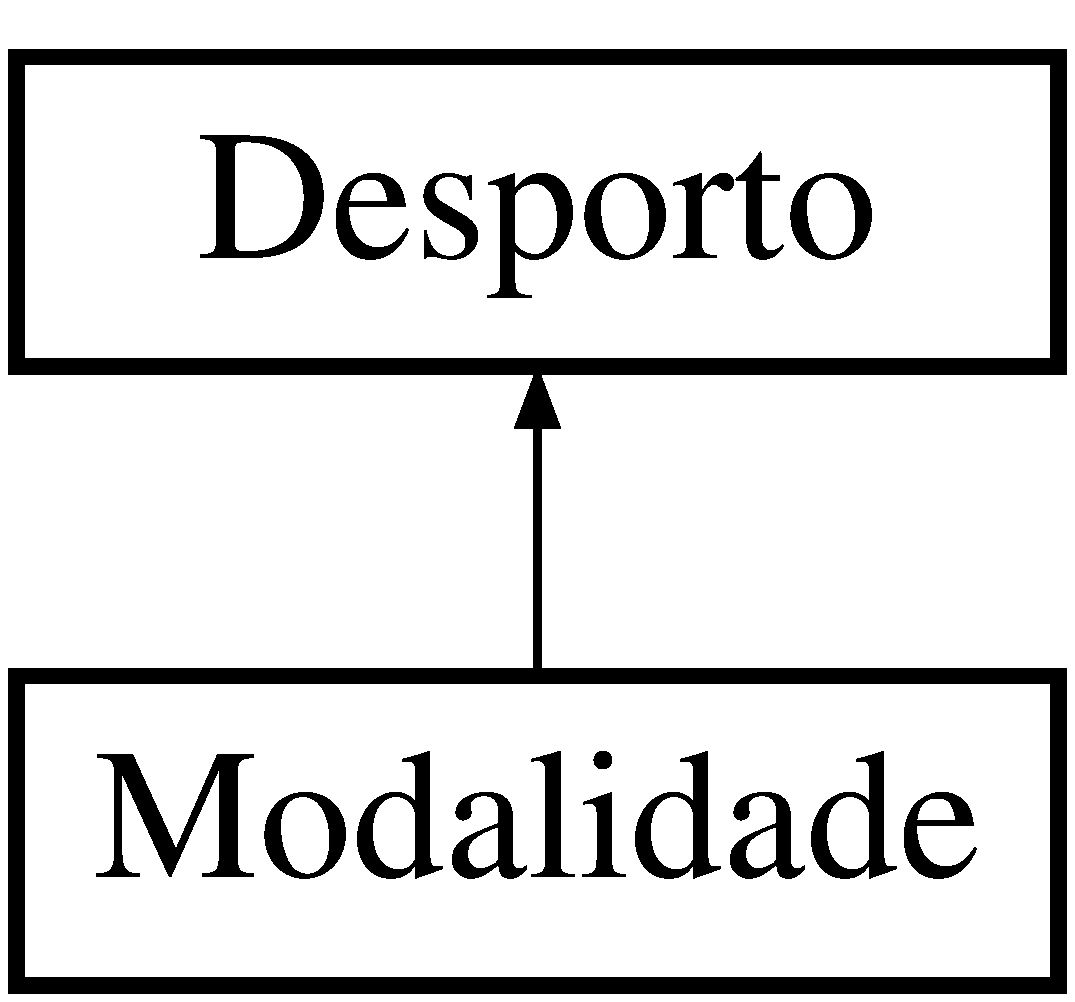
\includegraphics[height=2.000000cm]{class_modalidade}
\end{center}
\end{figure}
\subsection*{Public Member Functions}
\begin{DoxyCompactItemize}
\item 
\hyperlink{class_modalidade_a7d4201d3b89eb76cc5d147b642d32e72}{Modalidade} (string n, bool s)
\item 
\hyperlink{class_modalidade_aa60765d8148536471b4429e48858f883}{Modalidade} ()
\item 
virtual \hyperlink{class_modalidade_aea7526674a2128f030f58b8eff7c64bd}{$\sim$\+Modalidade} ()
\item 
string \hyperlink{class_modalidade_a46003f6a0dceac894f92971a6df9e4a7}{get\+Nome} () const 
\item 
string \hyperlink{class_modalidade_ac3326eec4d00a080b289ca249aa90cb7}{get\+Nome\+Desporto} () const 
\item 
bool \hyperlink{class_modalidade_acd8247f33c0aacef9388a2e452c06a19}{get\+Singular} () const 
\item 
unsigned int \hyperlink{class_modalidade_ae9016743d83bb1bd83ae1c076db5e65c}{get\+N\+Jogadores} () const 
\item 
string \hyperlink{class_modalidade_af7a45f3b8d73d45fd5cac46939344071}{pontuacao} (string \hyperlink{main_8h_a94bd6f24df224a4dd936a7dba7521ff0}{e1}, string e2)
\item 
bool \hyperlink{class_modalidade_a9f95f0d277728324be424570d69fc653}{operator==} (const \hyperlink{class_modalidade}{Modalidade} \&mod)
\end{DoxyCompactItemize}
\subsection*{Private Attributes}
\begin{DoxyCompactItemize}
\item 
string \hyperlink{class_modalidade_aaff7ae66117d1ee2bc9754bc45713c7e}{nome}
\item 
bool \hyperlink{class_modalidade_aaaea707c4eb8b1c6271d8ecafe09799f}{singular}
\item 
unsigned int \hyperlink{class_modalidade_a2ad080095c3fc56d05cbca69048a2704}{n\+Jogadores}
\end{DoxyCompactItemize}


\subsection{Constructor \& Destructor Documentation}
\hypertarget{class_modalidade_a7d4201d3b89eb76cc5d147b642d32e72}{}\index{Modalidade@{Modalidade}!Modalidade@{Modalidade}}
\index{Modalidade@{Modalidade}!Modalidade@{Modalidade}}
\subsubsection[{Modalidade(string n, bool s)}]{\setlength{\rightskip}{0pt plus 5cm}Modalidade\+::\+Modalidade (
\begin{DoxyParamCaption}
\item[{string}]{n, }
\item[{bool}]{s}
\end{DoxyParamCaption}
)}\label{class_modalidade_a7d4201d3b89eb76cc5d147b642d32e72}
\hypertarget{class_modalidade_aa60765d8148536471b4429e48858f883}{}\index{Modalidade@{Modalidade}!Modalidade@{Modalidade}}
\index{Modalidade@{Modalidade}!Modalidade@{Modalidade}}
\subsubsection[{Modalidade()}]{\setlength{\rightskip}{0pt plus 5cm}Modalidade\+::\+Modalidade (
\begin{DoxyParamCaption}
{}
\end{DoxyParamCaption}
)\hspace{0.3cm}{\ttfamily [inline]}}\label{class_modalidade_aa60765d8148536471b4429e48858f883}
\hypertarget{class_modalidade_aea7526674a2128f030f58b8eff7c64bd}{}\index{Modalidade@{Modalidade}!````~Modalidade@{$\sim$\+Modalidade}}
\index{````~Modalidade@{$\sim$\+Modalidade}!Modalidade@{Modalidade}}
\subsubsection[{$\sim$\+Modalidade()}]{\setlength{\rightskip}{0pt plus 5cm}Modalidade\+::$\sim$\+Modalidade (
\begin{DoxyParamCaption}
{}
\end{DoxyParamCaption}
)\hspace{0.3cm}{\ttfamily [virtual]}}\label{class_modalidade_aea7526674a2128f030f58b8eff7c64bd}


\subsection{Member Function Documentation}
\hypertarget{class_modalidade_ae9016743d83bb1bd83ae1c076db5e65c}{}\index{Modalidade@{Modalidade}!get\+N\+Jogadores@{get\+N\+Jogadores}}
\index{get\+N\+Jogadores@{get\+N\+Jogadores}!Modalidade@{Modalidade}}
\subsubsection[{get\+N\+Jogadores() const }]{\setlength{\rightskip}{0pt plus 5cm}unsigned int Modalidade\+::get\+N\+Jogadores (
\begin{DoxyParamCaption}
{}
\end{DoxyParamCaption}
) const\hspace{0.3cm}{\ttfamily [virtual]}}\label{class_modalidade_ae9016743d83bb1bd83ae1c076db5e65c}


Implements \hyperlink{class_desporto_ab03f722e71568b7235c9499876f849c6}{Desporto}.

\hypertarget{class_modalidade_a46003f6a0dceac894f92971a6df9e4a7}{}\index{Modalidade@{Modalidade}!get\+Nome@{get\+Nome}}
\index{get\+Nome@{get\+Nome}!Modalidade@{Modalidade}}
\subsubsection[{get\+Nome() const }]{\setlength{\rightskip}{0pt plus 5cm}string Modalidade\+::get\+Nome (
\begin{DoxyParamCaption}
{}
\end{DoxyParamCaption}
) const\hspace{0.3cm}{\ttfamily [virtual]}}\label{class_modalidade_a46003f6a0dceac894f92971a6df9e4a7}


Reimplemented from \hyperlink{class_desporto_ac55230ea2713d66a7e1c3e8731a4b601}{Desporto}.

\hypertarget{class_modalidade_ac3326eec4d00a080b289ca249aa90cb7}{}\index{Modalidade@{Modalidade}!get\+Nome\+Desporto@{get\+Nome\+Desporto}}
\index{get\+Nome\+Desporto@{get\+Nome\+Desporto}!Modalidade@{Modalidade}}
\subsubsection[{get\+Nome\+Desporto() const }]{\setlength{\rightskip}{0pt plus 5cm}string Modalidade\+::get\+Nome\+Desporto (
\begin{DoxyParamCaption}
{}
\end{DoxyParamCaption}
) const}\label{class_modalidade_ac3326eec4d00a080b289ca249aa90cb7}
\hypertarget{class_modalidade_acd8247f33c0aacef9388a2e452c06a19}{}\index{Modalidade@{Modalidade}!get\+Singular@{get\+Singular}}
\index{get\+Singular@{get\+Singular}!Modalidade@{Modalidade}}
\subsubsection[{get\+Singular() const }]{\setlength{\rightskip}{0pt plus 5cm}bool Modalidade\+::get\+Singular (
\begin{DoxyParamCaption}
{}
\end{DoxyParamCaption}
) const}\label{class_modalidade_acd8247f33c0aacef9388a2e452c06a19}
\hypertarget{class_modalidade_a9f95f0d277728324be424570d69fc653}{}\index{Modalidade@{Modalidade}!operator==@{operator==}}
\index{operator==@{operator==}!Modalidade@{Modalidade}}
\subsubsection[{operator==(const Modalidade \&mod)}]{\setlength{\rightskip}{0pt plus 5cm}bool Modalidade\+::operator== (
\begin{DoxyParamCaption}
\item[{const {\bf Modalidade} \&}]{mod}
\end{DoxyParamCaption}
)}\label{class_modalidade_a9f95f0d277728324be424570d69fc653}
\hypertarget{class_modalidade_af7a45f3b8d73d45fd5cac46939344071}{}\index{Modalidade@{Modalidade}!pontuacao@{pontuacao}}
\index{pontuacao@{pontuacao}!Modalidade@{Modalidade}}
\subsubsection[{pontuacao(string e1, string e2)}]{\setlength{\rightskip}{0pt plus 5cm}string Modalidade\+::pontuacao (
\begin{DoxyParamCaption}
\item[{string}]{e1, }
\item[{string}]{e2}
\end{DoxyParamCaption}
)}\label{class_modalidade_af7a45f3b8d73d45fd5cac46939344071}


\subsection{Member Data Documentation}
\hypertarget{class_modalidade_a2ad080095c3fc56d05cbca69048a2704}{}\index{Modalidade@{Modalidade}!n\+Jogadores@{n\+Jogadores}}
\index{n\+Jogadores@{n\+Jogadores}!Modalidade@{Modalidade}}
\subsubsection[{n\+Jogadores}]{\setlength{\rightskip}{0pt plus 5cm}unsigned int Modalidade\+::n\+Jogadores\hspace{0.3cm}{\ttfamily [private]}}\label{class_modalidade_a2ad080095c3fc56d05cbca69048a2704}
\hypertarget{class_modalidade_aaff7ae66117d1ee2bc9754bc45713c7e}{}\index{Modalidade@{Modalidade}!nome@{nome}}
\index{nome@{nome}!Modalidade@{Modalidade}}
\subsubsection[{nome}]{\setlength{\rightskip}{0pt plus 5cm}string Modalidade\+::nome\hspace{0.3cm}{\ttfamily [private]}}\label{class_modalidade_aaff7ae66117d1ee2bc9754bc45713c7e}
\hypertarget{class_modalidade_aaaea707c4eb8b1c6271d8ecafe09799f}{}\index{Modalidade@{Modalidade}!singular@{singular}}
\index{singular@{singular}!Modalidade@{Modalidade}}
\subsubsection[{singular}]{\setlength{\rightskip}{0pt plus 5cm}bool Modalidade\+::singular\hspace{0.3cm}{\ttfamily [private]}}\label{class_modalidade_aaaea707c4eb8b1c6271d8ecafe09799f}


The documentation for this class was generated from the following files\+:\begin{DoxyCompactItemize}
\item 
C\+:/\+Users/\+Alexandre/\+Git\+Hub/\+A\+E\+D\+A\+\_\+\+P\+R\+O\+J\+E\+C\+T\+O\+\_\+1/src/logic/\hyperlink{_modalidade_8h}{Modalidade.\+h}\item 
C\+:/\+Users/\+Alexandre/\+Git\+Hub/\+A\+E\+D\+A\+\_\+\+P\+R\+O\+J\+E\+C\+T\+O\+\_\+1/src/logic/\hyperlink{_modalidade_8cpp}{Modalidade.\+cpp}\end{DoxyCompactItemize}

\hypertarget{class_participante_inexistente}{}\section{Participante\+Inexistente Class Reference}
\label{class_participante_inexistente}\index{Participante\+Inexistente@{Participante\+Inexistente}}


{\ttfamily \#include $<$Utilities.\+h$>$}



The documentation for this class was generated from the following file\+:\begin{DoxyCompactItemize}
\item 
C\+:/\+Users/\+Alexandre/\+Git\+Hub/\+A\+E\+D\+A\+\_\+\+P\+R\+O\+J\+E\+C\+T\+O\+\_\+1/src/logic/\hyperlink{_utilities_8h}{Utilities.\+h}\end{DoxyCompactItemize}

\hypertarget{class_prova}{}\section{Prova Class Reference}
\label{class_prova}\index{Prova@{Prova}}


{\ttfamily \#include $<$Prova.\+h$>$}

\subsection*{Public Member Functions}
\begin{DoxyCompactItemize}
\item 
\hyperlink{class_prova_a4f36eaf2032327c06f7f7accd1ff7359}{Prova} ()
\item 
\hyperlink{class_prova_ab7713d18e28afa59ab2f106ec125d065}{Prova} (\hyperlink{structdate}{date} dat, string loc, unsigned int dur, vector$<$ \hyperlink{class_equipa}{Equipa} $\ast$ $>$ vs\+E, \hyperlink{class_modalidade}{Modalidade} $\ast$\hyperlink{class_prova_a9a372fdc63a673192aca93e5b3cdba22}{mod})
\item 
unsigned int \hyperlink{class_prova_a012b548cc9df64e2d43e59091796602f}{get\+I\+D} () const 
\item 
\hyperlink{structdate}{date} \hyperlink{class_prova_a88e20574edda3295f8dca8a06028348b}{get\+Data} () const 
\item 
void \hyperlink{class_prova_ad7b16cc7b4e09c0f0a149d3096eb66d4}{set\+Data} (\hyperlink{structdate}{date} d)
\item 
string \hyperlink{class_prova_a032f33dd9c442edda490029fff463898}{get\+Local} () const 
\item 
void \hyperlink{class_prova_a1d86cb87877a9dcaf3858078b12a4a7d}{set\+Local} (string l)
\item 
unsigned int \hyperlink{class_prova_aea1d2198c70bb49385f716df2addf7ae}{get\+Duracao} () const 
\item 
void \hyperlink{class_prova_addc2d33d4b2ef9ec2c7dfa66cefed083}{set\+Duracao} (unsigned int d)
\item 
vector$<$ \hyperlink{class_equipa}{Equipa} $\ast$ $>$ \hyperlink{class_prova_a015e691c4fa50bb756adced9cdc30eb7}{get\+Adversarios} () const 
\item 
void \hyperlink{class_prova_af805f91c0039ade3b1bab2ab0b43e592}{set\+Adversarios} (vector$<$ \hyperlink{class_equipa}{Equipa} $\ast$ $>$ v\+E)
\item 
\hyperlink{class_modalidade}{Modalidade} $\ast$ \hyperlink{class_prova_afbf918fbf8ddfd7a2b3785af51536e25}{get\+Modalidade} () const 
\item 
void \hyperlink{class_prova_aef40e220eca46c4fabc0a27b67768e3e}{set\+Modalidade} (\hyperlink{class_modalidade}{Modalidade} $\ast$m)
\item 
\hyperlink{class_equipa}{Equipa} $\ast$ \hyperlink{class_prova_a64d0727625b43e4382e4806c032b2868}{get\+Vencedor} () const 
\item 
void \hyperlink{class_prova_a97b48c140227e28e5a472f7b7bcedd07}{set\+Vencedor} (\hyperlink{class_equipa}{Equipa} $\ast$v)
\item 
bool \hyperlink{class_prova_a5f36832ceb6a8870f5f005cc2ceb5dd2}{get\+Completed} () const 
\item 
void \hyperlink{class_prova_a54eae0a267369ea33421d72418597386}{set\+Completed} (bool b)
\item 
bool \hyperlink{class_prova_a88b8cc8150bb374039a701a37101fbef}{get\+Prova\+Tempo} () const 
\item 
void \hyperlink{class_prova_afea493249261504dbb3629c5834831c8}{set\+Prova\+Temo} (bool b)
\item 
\hyperlink{class_atleta}{Atleta} $\ast$ \hyperlink{class_prova_a34d362f2cfa3c77966e0644203aae796}{get\+Participante} (int i) const 
\item 
string \hyperlink{class_prova_ae170e53e9684644c4cfb5c864413a8b7}{get\+Data\+Formatada} () const 
\item 
void \hyperlink{class_prova_a7bb057ccef0b2b0be425cecc6ab6545e}{print} ()
\item 
bool \hyperlink{class_prova_afc694469d1207f16ffb9525fe2ffda81}{operator!=} (const \hyperlink{class_prova}{Prova} \&p)
\end{DoxyCompactItemize}
\subsection*{Private Attributes}
\begin{DoxyCompactItemize}
\item 
int \hyperlink{class_prova_a23b51edf66d26661629b5330db67c3e7}{id}
\item 
\hyperlink{structdate}{date} \hyperlink{class_prova_a534b71e749122e706bbdd68e6b3410f4}{data}
\item 
string \hyperlink{class_prova_a4ff729b96dc2198a40d05dc7fdc38081}{local}
\item 
unsigned int \hyperlink{class_prova_a858c1f2a4be696df02eebe6419c34dc5}{duracao}
\item 
vector$<$ \hyperlink{class_equipa}{Equipa} $\ast$ $>$ \hyperlink{class_prova_aa085e9c4905e762142b6b735f4dfda30}{vs}
\item 
\hyperlink{class_modalidade}{Modalidade} $\ast$ \hyperlink{class_prova_a9a372fdc63a673192aca93e5b3cdba22}{mod}
\item 
\hyperlink{class_equipa}{Equipa} $\ast$ \hyperlink{class_prova_a9da09789da7cc0ef43b38197c96558fc}{vencedor}
\item 
bool \hyperlink{class_prova_a9b551ecafa591456d49345ceb9ea790d}{prova\+T}
\item 
bool \hyperlink{class_prova_aad473b9a0e23d11ba133ebdeea317522}{completed}
\end{DoxyCompactItemize}
\subsection*{Static Private Attributes}
\begin{DoxyCompactItemize}
\item 
static int \hyperlink{class_prova_aeaa338e40106c1be53f3f1134d3fb942}{new\+I\+D} = 0
\end{DoxyCompactItemize}


\subsection{Constructor \& Destructor Documentation}
\hypertarget{class_prova_a4f36eaf2032327c06f7f7accd1ff7359}{}\index{Prova@{Prova}!Prova@{Prova}}
\index{Prova@{Prova}!Prova@{Prova}}
\subsubsection[{Prova()}]{\setlength{\rightskip}{0pt plus 5cm}Prova\+::\+Prova (
\begin{DoxyParamCaption}
{}
\end{DoxyParamCaption}
)\hspace{0.3cm}{\ttfamily [inline]}}\label{class_prova_a4f36eaf2032327c06f7f7accd1ff7359}
\hypertarget{class_prova_ab7713d18e28afa59ab2f106ec125d065}{}\index{Prova@{Prova}!Prova@{Prova}}
\index{Prova@{Prova}!Prova@{Prova}}
\subsubsection[{Prova(date dat, string loc, unsigned int dur, vector$<$ Equipa $\ast$ $>$ vs\+E, Modalidade $\ast$mod)}]{\setlength{\rightskip}{0pt plus 5cm}Prova\+::\+Prova (
\begin{DoxyParamCaption}
\item[{{\bf date}}]{dat, }
\item[{string}]{loc, }
\item[{unsigned int}]{dur, }
\item[{vector$<$ {\bf Equipa} $\ast$ $>$}]{vs\+E, }
\item[{{\bf Modalidade} $\ast$}]{mod}
\end{DoxyParamCaption}
)}\label{class_prova_ab7713d18e28afa59ab2f106ec125d065}


\subsection{Member Function Documentation}
\hypertarget{class_prova_a015e691c4fa50bb756adced9cdc30eb7}{}\index{Prova@{Prova}!get\+Adversarios@{get\+Adversarios}}
\index{get\+Adversarios@{get\+Adversarios}!Prova@{Prova}}
\subsubsection[{get\+Adversarios() const }]{\setlength{\rightskip}{0pt plus 5cm}vector$<$ {\bf Equipa} $\ast$ $>$ Prova\+::get\+Adversarios (
\begin{DoxyParamCaption}
{}
\end{DoxyParamCaption}
) const}\label{class_prova_a015e691c4fa50bb756adced9cdc30eb7}
\hypertarget{class_prova_a5f36832ceb6a8870f5f005cc2ceb5dd2}{}\index{Prova@{Prova}!get\+Completed@{get\+Completed}}
\index{get\+Completed@{get\+Completed}!Prova@{Prova}}
\subsubsection[{get\+Completed() const }]{\setlength{\rightskip}{0pt plus 5cm}bool Prova\+::get\+Completed (
\begin{DoxyParamCaption}
{}
\end{DoxyParamCaption}
) const}\label{class_prova_a5f36832ceb6a8870f5f005cc2ceb5dd2}
\hypertarget{class_prova_a88e20574edda3295f8dca8a06028348b}{}\index{Prova@{Prova}!get\+Data@{get\+Data}}
\index{get\+Data@{get\+Data}!Prova@{Prova}}
\subsubsection[{get\+Data() const }]{\setlength{\rightskip}{0pt plus 5cm}{\bf date} Prova\+::get\+Data (
\begin{DoxyParamCaption}
{}
\end{DoxyParamCaption}
) const}\label{class_prova_a88e20574edda3295f8dca8a06028348b}
\hypertarget{class_prova_ae170e53e9684644c4cfb5c864413a8b7}{}\index{Prova@{Prova}!get\+Data\+Formatada@{get\+Data\+Formatada}}
\index{get\+Data\+Formatada@{get\+Data\+Formatada}!Prova@{Prova}}
\subsubsection[{get\+Data\+Formatada() const }]{\setlength{\rightskip}{0pt plus 5cm}string Prova\+::get\+Data\+Formatada (
\begin{DoxyParamCaption}
{}
\end{DoxyParamCaption}
) const}\label{class_prova_ae170e53e9684644c4cfb5c864413a8b7}
\hypertarget{class_prova_aea1d2198c70bb49385f716df2addf7ae}{}\index{Prova@{Prova}!get\+Duracao@{get\+Duracao}}
\index{get\+Duracao@{get\+Duracao}!Prova@{Prova}}
\subsubsection[{get\+Duracao() const }]{\setlength{\rightskip}{0pt plus 5cm}unsigned int Prova\+::get\+Duracao (
\begin{DoxyParamCaption}
{}
\end{DoxyParamCaption}
) const}\label{class_prova_aea1d2198c70bb49385f716df2addf7ae}
\hypertarget{class_prova_a012b548cc9df64e2d43e59091796602f}{}\index{Prova@{Prova}!get\+I\+D@{get\+I\+D}}
\index{get\+I\+D@{get\+I\+D}!Prova@{Prova}}
\subsubsection[{get\+I\+D() const }]{\setlength{\rightskip}{0pt plus 5cm}unsigned int Prova\+::get\+I\+D (
\begin{DoxyParamCaption}
{}
\end{DoxyParamCaption}
) const}\label{class_prova_a012b548cc9df64e2d43e59091796602f}
\hypertarget{class_prova_a032f33dd9c442edda490029fff463898}{}\index{Prova@{Prova}!get\+Local@{get\+Local}}
\index{get\+Local@{get\+Local}!Prova@{Prova}}
\subsubsection[{get\+Local() const }]{\setlength{\rightskip}{0pt plus 5cm}string Prova\+::get\+Local (
\begin{DoxyParamCaption}
{}
\end{DoxyParamCaption}
) const}\label{class_prova_a032f33dd9c442edda490029fff463898}
\hypertarget{class_prova_afbf918fbf8ddfd7a2b3785af51536e25}{}\index{Prova@{Prova}!get\+Modalidade@{get\+Modalidade}}
\index{get\+Modalidade@{get\+Modalidade}!Prova@{Prova}}
\subsubsection[{get\+Modalidade() const }]{\setlength{\rightskip}{0pt plus 5cm}{\bf Modalidade} $\ast$ Prova\+::get\+Modalidade (
\begin{DoxyParamCaption}
{}
\end{DoxyParamCaption}
) const}\label{class_prova_afbf918fbf8ddfd7a2b3785af51536e25}
\hypertarget{class_prova_a34d362f2cfa3c77966e0644203aae796}{}\index{Prova@{Prova}!get\+Participante@{get\+Participante}}
\index{get\+Participante@{get\+Participante}!Prova@{Prova}}
\subsubsection[{get\+Participante(int i) const }]{\setlength{\rightskip}{0pt plus 5cm}{\bf Atleta} $\ast$ Prova\+::get\+Participante (
\begin{DoxyParamCaption}
\item[{int}]{i}
\end{DoxyParamCaption}
) const}\label{class_prova_a34d362f2cfa3c77966e0644203aae796}
\hypertarget{class_prova_a88b8cc8150bb374039a701a37101fbef}{}\index{Prova@{Prova}!get\+Prova\+Tempo@{get\+Prova\+Tempo}}
\index{get\+Prova\+Tempo@{get\+Prova\+Tempo}!Prova@{Prova}}
\subsubsection[{get\+Prova\+Tempo() const }]{\setlength{\rightskip}{0pt plus 5cm}bool Prova\+::get\+Prova\+Tempo (
\begin{DoxyParamCaption}
{}
\end{DoxyParamCaption}
) const}\label{class_prova_a88b8cc8150bb374039a701a37101fbef}
\hypertarget{class_prova_a64d0727625b43e4382e4806c032b2868}{}\index{Prova@{Prova}!get\+Vencedor@{get\+Vencedor}}
\index{get\+Vencedor@{get\+Vencedor}!Prova@{Prova}}
\subsubsection[{get\+Vencedor() const }]{\setlength{\rightskip}{0pt plus 5cm}{\bf Equipa} $\ast$ Prova\+::get\+Vencedor (
\begin{DoxyParamCaption}
{}
\end{DoxyParamCaption}
) const}\label{class_prova_a64d0727625b43e4382e4806c032b2868}
\hypertarget{class_prova_afc694469d1207f16ffb9525fe2ffda81}{}\index{Prova@{Prova}!operator"!=@{operator"!=}}
\index{operator"!=@{operator"!=}!Prova@{Prova}}
\subsubsection[{operator"!=(const Prova \&p)}]{\setlength{\rightskip}{0pt plus 5cm}bool Prova\+::operator!= (
\begin{DoxyParamCaption}
\item[{const {\bf Prova} \&}]{p}
\end{DoxyParamCaption}
)}\label{class_prova_afc694469d1207f16ffb9525fe2ffda81}
\hypertarget{class_prova_a7bb057ccef0b2b0be425cecc6ab6545e}{}\index{Prova@{Prova}!print@{print}}
\index{print@{print}!Prova@{Prova}}
\subsubsection[{print()}]{\setlength{\rightskip}{0pt plus 5cm}void Prova\+::print (
\begin{DoxyParamCaption}
{}
\end{DoxyParamCaption}
)}\label{class_prova_a7bb057ccef0b2b0be425cecc6ab6545e}
\hypertarget{class_prova_af805f91c0039ade3b1bab2ab0b43e592}{}\index{Prova@{Prova}!set\+Adversarios@{set\+Adversarios}}
\index{set\+Adversarios@{set\+Adversarios}!Prova@{Prova}}
\subsubsection[{set\+Adversarios(vector$<$ Equipa $\ast$ $>$ v\+E)}]{\setlength{\rightskip}{0pt plus 5cm}void Prova\+::set\+Adversarios (
\begin{DoxyParamCaption}
\item[{vector$<$ {\bf Equipa} $\ast$ $>$}]{v\+E}
\end{DoxyParamCaption}
)}\label{class_prova_af805f91c0039ade3b1bab2ab0b43e592}
\hypertarget{class_prova_a54eae0a267369ea33421d72418597386}{}\index{Prova@{Prova}!set\+Completed@{set\+Completed}}
\index{set\+Completed@{set\+Completed}!Prova@{Prova}}
\subsubsection[{set\+Completed(bool b)}]{\setlength{\rightskip}{0pt plus 5cm}void Prova\+::set\+Completed (
\begin{DoxyParamCaption}
\item[{bool}]{b}
\end{DoxyParamCaption}
)}\label{class_prova_a54eae0a267369ea33421d72418597386}
\hypertarget{class_prova_ad7b16cc7b4e09c0f0a149d3096eb66d4}{}\index{Prova@{Prova}!set\+Data@{set\+Data}}
\index{set\+Data@{set\+Data}!Prova@{Prova}}
\subsubsection[{set\+Data(date d)}]{\setlength{\rightskip}{0pt plus 5cm}void Prova\+::set\+Data (
\begin{DoxyParamCaption}
\item[{{\bf date}}]{d}
\end{DoxyParamCaption}
)}\label{class_prova_ad7b16cc7b4e09c0f0a149d3096eb66d4}
\hypertarget{class_prova_addc2d33d4b2ef9ec2c7dfa66cefed083}{}\index{Prova@{Prova}!set\+Duracao@{set\+Duracao}}
\index{set\+Duracao@{set\+Duracao}!Prova@{Prova}}
\subsubsection[{set\+Duracao(unsigned int d)}]{\setlength{\rightskip}{0pt plus 5cm}void Prova\+::set\+Duracao (
\begin{DoxyParamCaption}
\item[{unsigned int}]{d}
\end{DoxyParamCaption}
)}\label{class_prova_addc2d33d4b2ef9ec2c7dfa66cefed083}
\hypertarget{class_prova_a1d86cb87877a9dcaf3858078b12a4a7d}{}\index{Prova@{Prova}!set\+Local@{set\+Local}}
\index{set\+Local@{set\+Local}!Prova@{Prova}}
\subsubsection[{set\+Local(string l)}]{\setlength{\rightskip}{0pt plus 5cm}void Prova\+::set\+Local (
\begin{DoxyParamCaption}
\item[{string}]{l}
\end{DoxyParamCaption}
)}\label{class_prova_a1d86cb87877a9dcaf3858078b12a4a7d}
\hypertarget{class_prova_aef40e220eca46c4fabc0a27b67768e3e}{}\index{Prova@{Prova}!set\+Modalidade@{set\+Modalidade}}
\index{set\+Modalidade@{set\+Modalidade}!Prova@{Prova}}
\subsubsection[{set\+Modalidade(\+Modalidade $\ast$m)}]{\setlength{\rightskip}{0pt plus 5cm}void Prova\+::set\+Modalidade (
\begin{DoxyParamCaption}
\item[{{\bf Modalidade} $\ast$}]{m}
\end{DoxyParamCaption}
)}\label{class_prova_aef40e220eca46c4fabc0a27b67768e3e}
\hypertarget{class_prova_afea493249261504dbb3629c5834831c8}{}\index{Prova@{Prova}!set\+Prova\+Temo@{set\+Prova\+Temo}}
\index{set\+Prova\+Temo@{set\+Prova\+Temo}!Prova@{Prova}}
\subsubsection[{set\+Prova\+Temo(bool b)}]{\setlength{\rightskip}{0pt plus 5cm}void Prova\+::set\+Prova\+Temo (
\begin{DoxyParamCaption}
\item[{bool}]{b}
\end{DoxyParamCaption}
)}\label{class_prova_afea493249261504dbb3629c5834831c8}
\hypertarget{class_prova_a97b48c140227e28e5a472f7b7bcedd07}{}\index{Prova@{Prova}!set\+Vencedor@{set\+Vencedor}}
\index{set\+Vencedor@{set\+Vencedor}!Prova@{Prova}}
\subsubsection[{set\+Vencedor(\+Equipa $\ast$v)}]{\setlength{\rightskip}{0pt plus 5cm}void Prova\+::set\+Vencedor (
\begin{DoxyParamCaption}
\item[{{\bf Equipa} $\ast$}]{v}
\end{DoxyParamCaption}
)}\label{class_prova_a97b48c140227e28e5a472f7b7bcedd07}


\subsection{Member Data Documentation}
\hypertarget{class_prova_aad473b9a0e23d11ba133ebdeea317522}{}\index{Prova@{Prova}!completed@{completed}}
\index{completed@{completed}!Prova@{Prova}}
\subsubsection[{completed}]{\setlength{\rightskip}{0pt plus 5cm}bool Prova\+::completed\hspace{0.3cm}{\ttfamily [private]}}\label{class_prova_aad473b9a0e23d11ba133ebdeea317522}
\hypertarget{class_prova_a534b71e749122e706bbdd68e6b3410f4}{}\index{Prova@{Prova}!data@{data}}
\index{data@{data}!Prova@{Prova}}
\subsubsection[{data}]{\setlength{\rightskip}{0pt plus 5cm}{\bf date} Prova\+::data\hspace{0.3cm}{\ttfamily [private]}}\label{class_prova_a534b71e749122e706bbdd68e6b3410f4}
\hypertarget{class_prova_a858c1f2a4be696df02eebe6419c34dc5}{}\index{Prova@{Prova}!duracao@{duracao}}
\index{duracao@{duracao}!Prova@{Prova}}
\subsubsection[{duracao}]{\setlength{\rightskip}{0pt plus 5cm}unsigned int Prova\+::duracao\hspace{0.3cm}{\ttfamily [private]}}\label{class_prova_a858c1f2a4be696df02eebe6419c34dc5}
\hypertarget{class_prova_a23b51edf66d26661629b5330db67c3e7}{}\index{Prova@{Prova}!id@{id}}
\index{id@{id}!Prova@{Prova}}
\subsubsection[{id}]{\setlength{\rightskip}{0pt plus 5cm}int Prova\+::id\hspace{0.3cm}{\ttfamily [private]}}\label{class_prova_a23b51edf66d26661629b5330db67c3e7}
\hypertarget{class_prova_a4ff729b96dc2198a40d05dc7fdc38081}{}\index{Prova@{Prova}!local@{local}}
\index{local@{local}!Prova@{Prova}}
\subsubsection[{local}]{\setlength{\rightskip}{0pt plus 5cm}string Prova\+::local\hspace{0.3cm}{\ttfamily [private]}}\label{class_prova_a4ff729b96dc2198a40d05dc7fdc38081}
\hypertarget{class_prova_a9a372fdc63a673192aca93e5b3cdba22}{}\index{Prova@{Prova}!mod@{mod}}
\index{mod@{mod}!Prova@{Prova}}
\subsubsection[{mod}]{\setlength{\rightskip}{0pt plus 5cm}{\bf Modalidade}$\ast$ Prova\+::mod\hspace{0.3cm}{\ttfamily [private]}}\label{class_prova_a9a372fdc63a673192aca93e5b3cdba22}
\hypertarget{class_prova_aeaa338e40106c1be53f3f1134d3fb942}{}\index{Prova@{Prova}!new\+I\+D@{new\+I\+D}}
\index{new\+I\+D@{new\+I\+D}!Prova@{Prova}}
\subsubsection[{new\+I\+D}]{\setlength{\rightskip}{0pt plus 5cm}int Prova\+::new\+I\+D = 0\hspace{0.3cm}{\ttfamily [static]}, {\ttfamily [private]}}\label{class_prova_aeaa338e40106c1be53f3f1134d3fb942}
\hypertarget{class_prova_a9b551ecafa591456d49345ceb9ea790d}{}\index{Prova@{Prova}!prova\+T@{prova\+T}}
\index{prova\+T@{prova\+T}!Prova@{Prova}}
\subsubsection[{prova\+T}]{\setlength{\rightskip}{0pt plus 5cm}bool Prova\+::prova\+T\hspace{0.3cm}{\ttfamily [private]}}\label{class_prova_a9b551ecafa591456d49345ceb9ea790d}
\hypertarget{class_prova_a9da09789da7cc0ef43b38197c96558fc}{}\index{Prova@{Prova}!vencedor@{vencedor}}
\index{vencedor@{vencedor}!Prova@{Prova}}
\subsubsection[{vencedor}]{\setlength{\rightskip}{0pt plus 5cm}{\bf Equipa}$\ast$ Prova\+::vencedor\hspace{0.3cm}{\ttfamily [private]}}\label{class_prova_a9da09789da7cc0ef43b38197c96558fc}
\hypertarget{class_prova_aa085e9c4905e762142b6b735f4dfda30}{}\index{Prova@{Prova}!vs@{vs}}
\index{vs@{vs}!Prova@{Prova}}
\subsubsection[{vs}]{\setlength{\rightskip}{0pt plus 5cm}vector$<${\bf Equipa}$\ast$$>$ Prova\+::vs\hspace{0.3cm}{\ttfamily [private]}}\label{class_prova_aa085e9c4905e762142b6b735f4dfda30}


The documentation for this class was generated from the following files\+:\begin{DoxyCompactItemize}
\item 
C\+:/\+Users/\+Alexandre/\+Git\+Hub/\+A\+E\+D\+A\+\_\+\+P\+R\+O\+J\+E\+C\+T\+O\+\_\+1/src/logic/\hyperlink{_prova_8h}{Prova.\+h}\item 
C\+:/\+Users/\+Alexandre/\+Git\+Hub/\+A\+E\+D\+A\+\_\+\+P\+R\+O\+J\+E\+C\+T\+O\+\_\+1/src/logic/\hyperlink{_prova_8cpp}{Prova.\+cpp}\end{DoxyCompactItemize}

\hypertarget{class_prova_inexistente}{}\section{Prova\+Inexistente Class Reference}
\label{class_prova_inexistente}\index{Prova\+Inexistente@{Prova\+Inexistente}}


{\ttfamily \#include $<$Utilities.\+h$>$}

\subsection*{Public Member Functions}
\begin{DoxyCompactItemize}
\item 
\hyperlink{class_prova_inexistente_aea24919e23d55c0910c15dfbc890b0ac}{Prova\+Inexistente} (int i)
\item 
int \hyperlink{class_prova_inexistente_a015299b9b54f200e95e482b094b99f86}{get\+I\+D} ()
\end{DoxyCompactItemize}
\subsection*{Public Attributes}
\begin{DoxyCompactItemize}
\item 
int \hyperlink{class_prova_inexistente_a5d0ff2e27cc6ebb2b52a4e91b68c3ebb}{id}
\end{DoxyCompactItemize}


\subsection{Constructor \& Destructor Documentation}
\hypertarget{class_prova_inexistente_aea24919e23d55c0910c15dfbc890b0ac}{}\index{Prova\+Inexistente@{Prova\+Inexistente}!Prova\+Inexistente@{Prova\+Inexistente}}
\index{Prova\+Inexistente@{Prova\+Inexistente}!Prova\+Inexistente@{Prova\+Inexistente}}
\subsubsection[{Prova\+Inexistente(int i)}]{\setlength{\rightskip}{0pt plus 5cm}Prova\+Inexistente\+::\+Prova\+Inexistente (
\begin{DoxyParamCaption}
\item[{int}]{i}
\end{DoxyParamCaption}
)\hspace{0.3cm}{\ttfamily [inline]}}\label{class_prova_inexistente_aea24919e23d55c0910c15dfbc890b0ac}


\subsection{Member Function Documentation}
\hypertarget{class_prova_inexistente_a015299b9b54f200e95e482b094b99f86}{}\index{Prova\+Inexistente@{Prova\+Inexistente}!get\+I\+D@{get\+I\+D}}
\index{get\+I\+D@{get\+I\+D}!Prova\+Inexistente@{Prova\+Inexistente}}
\subsubsection[{get\+I\+D()}]{\setlength{\rightskip}{0pt plus 5cm}int Prova\+Inexistente\+::get\+I\+D (
\begin{DoxyParamCaption}
{}
\end{DoxyParamCaption}
)\hspace{0.3cm}{\ttfamily [inline]}}\label{class_prova_inexistente_a015299b9b54f200e95e482b094b99f86}


\subsection{Member Data Documentation}
\hypertarget{class_prova_inexistente_a5d0ff2e27cc6ebb2b52a4e91b68c3ebb}{}\index{Prova\+Inexistente@{Prova\+Inexistente}!id@{id}}
\index{id@{id}!Prova\+Inexistente@{Prova\+Inexistente}}
\subsubsection[{id}]{\setlength{\rightskip}{0pt plus 5cm}int Prova\+Inexistente\+::id}\label{class_prova_inexistente_a5d0ff2e27cc6ebb2b52a4e91b68c3ebb}


The documentation for this class was generated from the following file\+:\begin{DoxyCompactItemize}
\item 
C\+:/\+Users/\+Alexandre/\+Git\+Hub/\+A\+E\+D\+A\+\_\+\+P\+R\+O\+J\+E\+C\+T\+O\+\_\+1/src/logic/\hyperlink{_utilities_8h}{Utilities.\+h}\end{DoxyCompactItemize}

\hypertarget{class_valor_invalido}{}\section{Valor\+Invalido Class Reference}
\label{class_valor_invalido}\index{Valor\+Invalido@{Valor\+Invalido}}


{\ttfamily \#include $<$Utilities.\+h$>$}

\subsection*{Public Member Functions}
\begin{DoxyCompactItemize}
\item 
\hyperlink{class_valor_invalido_a199b828bd45954617402cc9b3767d7fc}{Valor\+Invalido} (int \hyperlink{class_valor_invalido_ad4b72e875677802b68fb511bc504f67c}{v})
\item 
int \hyperlink{class_valor_invalido_a18c667f85e09fc11a16978ca1f29d6ea}{get\+Valor} ()
\end{DoxyCompactItemize}
\subsection*{Public Attributes}
\begin{DoxyCompactItemize}
\item 
int \hyperlink{class_valor_invalido_ad4b72e875677802b68fb511bc504f67c}{v}
\end{DoxyCompactItemize}


\subsection{Constructor \& Destructor Documentation}
\hypertarget{class_valor_invalido_a199b828bd45954617402cc9b3767d7fc}{}\index{Valor\+Invalido@{Valor\+Invalido}!Valor\+Invalido@{Valor\+Invalido}}
\index{Valor\+Invalido@{Valor\+Invalido}!Valor\+Invalido@{Valor\+Invalido}}
\subsubsection[{Valor\+Invalido(int v)}]{\setlength{\rightskip}{0pt plus 5cm}Valor\+Invalido\+::\+Valor\+Invalido (
\begin{DoxyParamCaption}
\item[{int}]{v}
\end{DoxyParamCaption}
)\hspace{0.3cm}{\ttfamily [inline]}}\label{class_valor_invalido_a199b828bd45954617402cc9b3767d7fc}


\subsection{Member Function Documentation}
\hypertarget{class_valor_invalido_a18c667f85e09fc11a16978ca1f29d6ea}{}\index{Valor\+Invalido@{Valor\+Invalido}!get\+Valor@{get\+Valor}}
\index{get\+Valor@{get\+Valor}!Valor\+Invalido@{Valor\+Invalido}}
\subsubsection[{get\+Valor()}]{\setlength{\rightskip}{0pt plus 5cm}int Valor\+Invalido\+::get\+Valor (
\begin{DoxyParamCaption}
{}
\end{DoxyParamCaption}
)\hspace{0.3cm}{\ttfamily [inline]}}\label{class_valor_invalido_a18c667f85e09fc11a16978ca1f29d6ea}


\subsection{Member Data Documentation}
\hypertarget{class_valor_invalido_ad4b72e875677802b68fb511bc504f67c}{}\index{Valor\+Invalido@{Valor\+Invalido}!v@{v}}
\index{v@{v}!Valor\+Invalido@{Valor\+Invalido}}
\subsubsection[{v}]{\setlength{\rightskip}{0pt plus 5cm}int Valor\+Invalido\+::v}\label{class_valor_invalido_ad4b72e875677802b68fb511bc504f67c}


The documentation for this class was generated from the following file\+:\begin{DoxyCompactItemize}
\item 
C\+:/\+Users/\+Alexandre/\+Git\+Hub/\+A\+E\+D\+A\+\_\+\+P\+R\+O\+J\+E\+C\+T\+O\+\_\+1/src/logic/\hyperlink{_utilities_8h}{Utilities.\+h}\end{DoxyCompactItemize}

\chapter{File Documentation}
\hypertarget{_adepto_8cpp}{}\section{C\+:/\+Users/\+Alexandre/\+Git\+Hub/\+A\+E\+D\+A\+\_\+\+P\+R\+O\+J\+E\+C\+T\+O\+\_\+1/src/logic/\+Adepto.cpp File Reference}
\label{_adepto_8cpp}\index{C\+:/\+Users/\+Alexandre/\+Git\+Hub/\+A\+E\+D\+A\+\_\+\+P\+R\+O\+J\+E\+C\+T\+O\+\_\+1/src/logic/\+Adepto.\+cpp@{C\+:/\+Users/\+Alexandre/\+Git\+Hub/\+A\+E\+D\+A\+\_\+\+P\+R\+O\+J\+E\+C\+T\+O\+\_\+1/src/logic/\+Adepto.\+cpp}}
{\ttfamily \#include \char`\"{}Adepto.\+h\char`\"{}}\\*

\hypertarget{_adepto_8h}{}\section{C\+:/\+Users/\+Alexandre/\+Git\+Hub/\+A\+E\+D\+A\+\_\+\+P\+R\+O\+J\+E\+C\+T\+O\+\_\+1/src/logic/\+Adepto.h File Reference}
\label{_adepto_8h}\index{C\+:/\+Users/\+Alexandre/\+Git\+Hub/\+A\+E\+D\+A\+\_\+\+P\+R\+O\+J\+E\+C\+T\+O\+\_\+1/src/logic/\+Adepto.\+h@{C\+:/\+Users/\+Alexandre/\+Git\+Hub/\+A\+E\+D\+A\+\_\+\+P\+R\+O\+J\+E\+C\+T\+O\+\_\+1/src/logic/\+Adepto.\+h}}
{\ttfamily \#include $<$iostream$>$}\\*
{\ttfamily \#include $<$vector$>$}\\*
{\ttfamily \#include $<$string$>$}\\*
{\ttfamily \#include $<$fstream$>$}\\*
{\ttfamily \#include $<$ctime$>$}\\*
{\ttfamily \#include $<$sstream$>$}\\*
{\ttfamily \#include $<$stdlib.\+h$>$}\\*
\subsection*{Classes}
\begin{DoxyCompactItemize}
\item 
class \hyperlink{class_adepto}{Adepto}
\end{DoxyCompactItemize}

\hypertarget{_atleta_8cpp}{}\section{C\+:/\+Users/\+Alexandre/\+Git\+Hub/\+A\+E\+D\+A\+\_\+\+P\+R\+O\+J\+E\+C\+T\+O\+\_\+1/src/logic/\+Atleta.cpp File Reference}
\label{_atleta_8cpp}\index{C\+:/\+Users/\+Alexandre/\+Git\+Hub/\+A\+E\+D\+A\+\_\+\+P\+R\+O\+J\+E\+C\+T\+O\+\_\+1/src/logic/\+Atleta.\+cpp@{C\+:/\+Users/\+Alexandre/\+Git\+Hub/\+A\+E\+D\+A\+\_\+\+P\+R\+O\+J\+E\+C\+T\+O\+\_\+1/src/logic/\+Atleta.\+cpp}}
{\ttfamily \#include $<$iostream$>$}\\*
{\ttfamily \#include \char`\"{}Atleta.\+h\char`\"{}}\\*

\hypertarget{_atleta_8h}{}\section{C\+:/\+Users/\+Alexandre/\+Git\+Hub/\+A\+E\+D\+A\+\_\+\+P\+R\+O\+J\+E\+C\+T\+O\+\_\+1/src/logic/\+Atleta.h File Reference}
\label{_atleta_8h}\index{C\+:/\+Users/\+Alexandre/\+Git\+Hub/\+A\+E\+D\+A\+\_\+\+P\+R\+O\+J\+E\+C\+T\+O\+\_\+1/src/logic/\+Atleta.\+h@{C\+:/\+Users/\+Alexandre/\+Git\+Hub/\+A\+E\+D\+A\+\_\+\+P\+R\+O\+J\+E\+C\+T\+O\+\_\+1/src/logic/\+Atleta.\+h}}
{\ttfamily \#include $<$tr1/unordered\+\_\+set$>$}\\*
{\ttfamily \#include $<$vector$>$}\\*
{\ttfamily \#include $<$string$>$}\\*
{\ttfamily \#include $<$fstream$>$}\\*
{\ttfamily \#include $<$ctime$>$}\\*
{\ttfamily \#include $<$sstream$>$}\\*
{\ttfamily \#include $<$stdlib.\+h$>$}\\*
{\ttfamily \#include \char`\"{}Utilities.\+h\char`\"{}}\\*
{\ttfamily \#include \char`\"{}Modalidade.\+h\char`\"{}}\\*
\subsection*{Classes}
\begin{DoxyCompactItemize}
\item 
class \hyperlink{class_atleta}{Atleta}
\item 
struct \hyperlink{structhash__atletas}{hash\+\_\+atletas}
\item 
class \hyperlink{class_atletas_guardados}{Atletas\+Guardados}
\item 
class \hyperlink{class_atletas_guardados_1_1_erro_no_ficheiro}{Atletas\+Guardados\+::\+Erro\+No\+Ficheiro}
\end{DoxyCompactItemize}
\subsection*{Typedefs}
\begin{DoxyCompactItemize}
\item 
typedef tr1\+::unordered\+\_\+set$<$ \hyperlink{class_atleta}{Atleta}, \hyperlink{structhash__atletas}{hash\+\_\+atletas}, \hyperlink{structhash__atletas}{hash\+\_\+atletas} $>$ \hyperlink{_atleta_8h_a989ebe08ebb28dadcb4325cf4cb123dc}{Tabela}
\end{DoxyCompactItemize}


\subsection{Typedef Documentation}
\hypertarget{_atleta_8h_a989ebe08ebb28dadcb4325cf4cb123dc}{}\index{Atleta.\+h@{Atleta.\+h}!Tabela@{Tabela}}
\index{Tabela@{Tabela}!Atleta.\+h@{Atleta.\+h}}
\subsubsection[{Tabela}]{\setlength{\rightskip}{0pt plus 5cm}typedef tr1\+::unordered\+\_\+set$<${\bf Atleta}, {\bf hash\+\_\+atletas}, {\bf hash\+\_\+atletas}$>$ {\bf Tabela}}\label{_atleta_8h_a989ebe08ebb28dadcb4325cf4cb123dc}

\hypertarget{_bilhete_8cpp}{}\section{C\+:/\+Users/\+Alexandre/\+Git\+Hub/\+A\+E\+D\+A\+\_\+\+P\+R\+O\+J\+E\+C\+T\+O\+\_\+1/src/logic/\+Bilhete.cpp File Reference}
\label{_bilhete_8cpp}\index{C\+:/\+Users/\+Alexandre/\+Git\+Hub/\+A\+E\+D\+A\+\_\+\+P\+R\+O\+J\+E\+C\+T\+O\+\_\+1/src/logic/\+Bilhete.\+cpp@{C\+:/\+Users/\+Alexandre/\+Git\+Hub/\+A\+E\+D\+A\+\_\+\+P\+R\+O\+J\+E\+C\+T\+O\+\_\+1/src/logic/\+Bilhete.\+cpp}}
{\ttfamily \#include \char`\"{}Bilhete.\+h\char`\"{}}\\*

\hypertarget{_bilhete_8h}{}\section{C\+:/\+Users/\+Alexandre/\+Git\+Hub/\+A\+E\+D\+A\+\_\+\+P\+R\+O\+J\+E\+C\+T\+O\+\_\+1/src/logic/\+Bilhete.h File Reference}
\label{_bilhete_8h}\index{C\+:/\+Users/\+Alexandre/\+Git\+Hub/\+A\+E\+D\+A\+\_\+\+P\+R\+O\+J\+E\+C\+T\+O\+\_\+1/src/logic/\+Bilhete.\+h@{C\+:/\+Users/\+Alexandre/\+Git\+Hub/\+A\+E\+D\+A\+\_\+\+P\+R\+O\+J\+E\+C\+T\+O\+\_\+1/src/logic/\+Bilhete.\+h}}
{\ttfamily \#include $<$tr1/unordered\+\_\+set$>$}\\*
{\ttfamily \#include $<$vector$>$}\\*
{\ttfamily \#include $<$string$>$}\\*
{\ttfamily \#include $<$iostream$>$}\\*
{\ttfamily \#include $<$sstream$>$}\\*
{\ttfamily \#include $<$fstream$>$}\\*
{\ttfamily \#include $<$cstdlib$>$}\\*
{\ttfamily \#include \char`\"{}Utilities.\+h\char`\"{}}\\*
{\ttfamily \#include \char`\"{}Prova.\+h\char`\"{}}\\*
{\ttfamily \#include \char`\"{}Adepto.\+h\char`\"{}}\\*
\subsection*{Classes}
\begin{DoxyCompactItemize}
\item 
class \hyperlink{class_bilhete}{Bilhete}
\end{DoxyCompactItemize}

\hypertarget{_b_s_t_8h}{}\section{C\+:/\+Users/\+Alexandre/\+Git\+Hub/\+A\+E\+D\+A\+\_\+\+P\+R\+O\+J\+E\+C\+T\+O\+\_\+1/src/logic/\+B\+S\+T.h File Reference}
\label{_b_s_t_8h}\index{C\+:/\+Users/\+Alexandre/\+Git\+Hub/\+A\+E\+D\+A\+\_\+\+P\+R\+O\+J\+E\+C\+T\+O\+\_\+1/src/logic/\+B\+S\+T.\+h@{C\+:/\+Users/\+Alexandre/\+Git\+Hub/\+A\+E\+D\+A\+\_\+\+P\+R\+O\+J\+E\+C\+T\+O\+\_\+1/src/logic/\+B\+S\+T.\+h}}
{\ttfamily \#include $<$iostream$>$}\\*
{\ttfamily \#include $<$stack$>$}\\*
{\ttfamily \#include $<$queue$>$}\\*
\subsection*{Classes}
\begin{DoxyCompactItemize}
\item 
class \hyperlink{class_b_s_t_itr_in}{B\+S\+T\+Itr\+In$<$ Comparable $>$}
\item 
class \hyperlink{class_b_s_t_itr_pre}{B\+S\+T\+Itr\+Pre$<$ Comparable $>$}
\item 
class \hyperlink{class_b_s_t_itr_post}{B\+S\+T\+Itr\+Post$<$ Comparable $>$}
\item 
class \hyperlink{class_b_s_t_itr_level}{B\+S\+T\+Itr\+Level$<$ Comparable $>$}
\item 
class \hyperlink{class_b_s_t}{B\+S\+T$<$ Comparable $>$}
\item 
class \hyperlink{class_binary_node}{Binary\+Node$<$ Comparable $>$}
\item 
class \hyperlink{class_b_s_t}{B\+S\+T$<$ Comparable $>$}
\item 
class \hyperlink{class_b_s_t_itr_post}{B\+S\+T\+Itr\+Post$<$ Comparable $>$}
\item 
class \hyperlink{class_b_s_t_itr_pre}{B\+S\+T\+Itr\+Pre$<$ Comparable $>$}
\item 
class \hyperlink{class_b_s_t_itr_in}{B\+S\+T\+Itr\+In$<$ Comparable $>$}
\item 
class \hyperlink{class_b_s_t_itr_level}{B\+S\+T\+Itr\+Level$<$ Comparable $>$}
\end{DoxyCompactItemize}

\hypertarget{_calendario_8cpp}{}\section{C\+:/\+Users/\+Alexandre/\+Git\+Hub/\+A\+E\+D\+A\+\_\+\+P\+R\+O\+J\+E\+C\+T\+O\+\_\+1/src/logic/\+Calendario.cpp File Reference}
\label{_calendario_8cpp}\index{C\+:/\+Users/\+Alexandre/\+Git\+Hub/\+A\+E\+D\+A\+\_\+\+P\+R\+O\+J\+E\+C\+T\+O\+\_\+1/src/logic/\+Calendario.\+cpp@{C\+:/\+Users/\+Alexandre/\+Git\+Hub/\+A\+E\+D\+A\+\_\+\+P\+R\+O\+J\+E\+C\+T\+O\+\_\+1/src/logic/\+Calendario.\+cpp}}
{\ttfamily \#include \char`\"{}Calendario.\+h\char`\"{}}\\*
{\ttfamily \#include $<$iomanip$>$}\\*

\hypertarget{_calendario_8h}{}\section{C\+:/\+Users/\+Alexandre/\+Git\+Hub/\+A\+E\+D\+A\+\_\+\+P\+R\+O\+J\+E\+C\+T\+O\+\_\+1/src/logic/\+Calendario.h File Reference}
\label{_calendario_8h}\index{C\+:/\+Users/\+Alexandre/\+Git\+Hub/\+A\+E\+D\+A\+\_\+\+P\+R\+O\+J\+E\+C\+T\+O\+\_\+1/src/logic/\+Calendario.\+h@{C\+:/\+Users/\+Alexandre/\+Git\+Hub/\+A\+E\+D\+A\+\_\+\+P\+R\+O\+J\+E\+C\+T\+O\+\_\+1/src/logic/\+Calendario.\+h}}
{\ttfamily \#include $<$string$>$}\\*
{\ttfamily \#include $<$vector$>$}\\*
{\ttfamily \#include \char`\"{}B\+S\+T.\+h\char`\"{}}\\*
{\ttfamily \#include \char`\"{}Prova.\+h\char`\"{}}\\*
{\ttfamily \#include \char`\"{}Campeonato.\+h\char`\"{}}\\*
\subsection*{Classes}
\begin{DoxyCompactItemize}
\item 
class \hyperlink{class_calendario}{Calendario}
\end{DoxyCompactItemize}

\hypertarget{_campeonato_8cpp}{}\section{C\+:/\+Users/\+Alexandre/\+Git\+Hub/\+A\+E\+D\+A\+\_\+\+P\+R\+O\+J\+E\+C\+T\+O\+\_\+1/src/logic/\+Campeonato.cpp File Reference}
\label{_campeonato_8cpp}\index{C\+:/\+Users/\+Alexandre/\+Git\+Hub/\+A\+E\+D\+A\+\_\+\+P\+R\+O\+J\+E\+C\+T\+O\+\_\+1/src/logic/\+Campeonato.\+cpp@{C\+:/\+Users/\+Alexandre/\+Git\+Hub/\+A\+E\+D\+A\+\_\+\+P\+R\+O\+J\+E\+C\+T\+O\+\_\+1/src/logic/\+Campeonato.\+cpp}}
{\ttfamily \#include \char`\"{}Campeonato.\+h\char`\"{}}\\*

\hypertarget{_campeonato_8h}{}\section{C\+:/\+Users/\+Alexandre/\+Git\+Hub/\+A\+E\+D\+A\+\_\+\+P\+R\+O\+J\+E\+C\+T\+O\+\_\+1/src/logic/\+Campeonato.h File Reference}
\label{_campeonato_8h}\index{C\+:/\+Users/\+Alexandre/\+Git\+Hub/\+A\+E\+D\+A\+\_\+\+P\+R\+O\+J\+E\+C\+T\+O\+\_\+1/src/logic/\+Campeonato.\+h@{C\+:/\+Users/\+Alexandre/\+Git\+Hub/\+A\+E\+D\+A\+\_\+\+P\+R\+O\+J\+E\+C\+T\+O\+\_\+1/src/logic/\+Campeonato.\+h}}
{\ttfamily \#include $<$vector$>$}\\*
{\ttfamily \#include $<$string$>$}\\*
{\ttfamily \#include \char`\"{}Equipa.\+h\char`\"{}}\\*
{\ttfamily \#include \char`\"{}Desporto.\+h\char`\"{}}\\*
{\ttfamily \#include \char`\"{}Calendario.\+h\char`\"{}}\\*
{\ttfamily \#include \char`\"{}Utilities.\+h\char`\"{}}\\*
{\ttfamily \#include \char`\"{}Atleta.\+h\char`\"{}}\\*
{\ttfamily \#include $<$iostream$>$}\\*
\subsection*{Classes}
\begin{DoxyCompactItemize}
\item 
class \hyperlink{class_campeonato}{Campeonato}
\end{DoxyCompactItemize}

\hypertarget{_desporto_8h}{}\section{C\+:/\+Users/\+Alexandre/\+Git\+Hub/\+A\+E\+D\+A\+\_\+\+P\+R\+O\+J\+E\+C\+T\+O\+\_\+1/src/logic/\+Desporto.h File Reference}
\label{_desporto_8h}\index{C\+:/\+Users/\+Alexandre/\+Git\+Hub/\+A\+E\+D\+A\+\_\+\+P\+R\+O\+J\+E\+C\+T\+O\+\_\+1/src/logic/\+Desporto.\+h@{C\+:/\+Users/\+Alexandre/\+Git\+Hub/\+A\+E\+D\+A\+\_\+\+P\+R\+O\+J\+E\+C\+T\+O\+\_\+1/src/logic/\+Desporto.\+h}}
{\ttfamily \#include $<$vector$>$}\\*
{\ttfamily \#include $<$string$>$}\\*
\subsection*{Classes}
\begin{DoxyCompactItemize}
\item 
class \hyperlink{class_desporto}{Desporto}
\end{DoxyCompactItemize}

\hypertarget{_equipa_8cpp}{}\section{C\+:/\+Users/\+Alexandre/\+Git\+Hub/\+A\+E\+D\+A\+\_\+\+P\+R\+O\+J\+E\+C\+T\+O\+\_\+1/src/logic/\+Equipa.cpp File Reference}
\label{_equipa_8cpp}\index{C\+:/\+Users/\+Alexandre/\+Git\+Hub/\+A\+E\+D\+A\+\_\+\+P\+R\+O\+J\+E\+C\+T\+O\+\_\+1/src/logic/\+Equipa.\+cpp@{C\+:/\+Users/\+Alexandre/\+Git\+Hub/\+A\+E\+D\+A\+\_\+\+P\+R\+O\+J\+E\+C\+T\+O\+\_\+1/src/logic/\+Equipa.\+cpp}}
{\ttfamily \#include $<$iostream$>$}\\*
{\ttfamily \#include $<$iterator$>$}\\*
{\ttfamily \#include \char`\"{}Equipa.\+h\char`\"{}}\\*

\hypertarget{_equipa_8h}{}\section{C\+:/\+Users/\+Alexandre/\+Git\+Hub/\+A\+E\+D\+A\+\_\+\+P\+R\+O\+J\+E\+C\+T\+O\+\_\+1/src/logic/\+Equipa.h File Reference}
\label{_equipa_8h}\index{C\+:/\+Users/\+Alexandre/\+Git\+Hub/\+A\+E\+D\+A\+\_\+\+P\+R\+O\+J\+E\+C\+T\+O\+\_\+1/src/logic/\+Equipa.\+h@{C\+:/\+Users/\+Alexandre/\+Git\+Hub/\+A\+E\+D\+A\+\_\+\+P\+R\+O\+J\+E\+C\+T\+O\+\_\+1/src/logic/\+Equipa.\+h}}
{\ttfamily \#include $<$vector$>$}\\*
{\ttfamily \#include $<$string$>$}\\*
{\ttfamily \#include $<$iostream$>$}\\*
{\ttfamily \#include $<$sstream$>$}\\*
{\ttfamily \#include $<$fstream$>$}\\*
{\ttfamily \#include $<$cstdlib$>$}\\*
{\ttfamily \#include \char`\"{}Atleta.\+h\char`\"{}}\\*
\subsection*{Classes}
\begin{DoxyCompactItemize}
\item 
class \hyperlink{class_equipa}{Equipa}
\item 
struct \hyperlink{struct_compara_equipa}{Compara\+Equipa}
\end{DoxyCompactItemize}

\hypertarget{_lists_8cpp}{}\section{C\+:/\+Users/\+Alexandre/\+Git\+Hub/\+A\+E\+D\+A\+\_\+\+P\+R\+O\+J\+E\+C\+T\+O\+\_\+1/src/logic/\+Lists.cpp File Reference}
\label{_lists_8cpp}\index{C\+:/\+Users/\+Alexandre/\+Git\+Hub/\+A\+E\+D\+A\+\_\+\+P\+R\+O\+J\+E\+C\+T\+O\+\_\+1/src/logic/\+Lists.\+cpp@{C\+:/\+Users/\+Alexandre/\+Git\+Hub/\+A\+E\+D\+A\+\_\+\+P\+R\+O\+J\+E\+C\+T\+O\+\_\+1/src/logic/\+Lists.\+cpp}}

\hypertarget{_lists_8h}{}\section{C\+:/\+Users/\+Alexandre/\+Git\+Hub/\+A\+E\+D\+A\+\_\+\+P\+R\+O\+J\+E\+C\+T\+O\+\_\+1/src/logic/\+Lists.h File Reference}
\label{_lists_8h}\index{C\+:/\+Users/\+Alexandre/\+Git\+Hub/\+A\+E\+D\+A\+\_\+\+P\+R\+O\+J\+E\+C\+T\+O\+\_\+1/src/logic/\+Lists.\+h@{C\+:/\+Users/\+Alexandre/\+Git\+Hub/\+A\+E\+D\+A\+\_\+\+P\+R\+O\+J\+E\+C\+T\+O\+\_\+1/src/logic/\+Lists.\+h}}

\hypertarget{main_8cpp}{}\section{C\+:/\+Users/\+Alexandre/\+Git\+Hub/\+A\+E\+D\+A\+\_\+\+P\+R\+O\+J\+E\+C\+T\+O\+\_\+1/src/logic/main.cpp File Reference}
\label{main_8cpp}\index{C\+:/\+Users/\+Alexandre/\+Git\+Hub/\+A\+E\+D\+A\+\_\+\+P\+R\+O\+J\+E\+C\+T\+O\+\_\+1/src/logic/main.\+cpp@{C\+:/\+Users/\+Alexandre/\+Git\+Hub/\+A\+E\+D\+A\+\_\+\+P\+R\+O\+J\+E\+C\+T\+O\+\_\+1/src/logic/main.\+cpp}}
{\ttfamily \#include \char`\"{}Menu.\+h\char`\"{}}\\*
\subsection*{Functions}
\begin{DoxyCompactItemize}
\item 
int \hyperlink{main_8cpp_ae66f6b31b5ad750f1fe042a706a4e3d4}{main} ()
\end{DoxyCompactItemize}


\subsection{Function Documentation}
\hypertarget{main_8cpp_ae66f6b31b5ad750f1fe042a706a4e3d4}{}\index{main.\+cpp@{main.\+cpp}!main@{main}}
\index{main@{main}!main.\+cpp@{main.\+cpp}}
\subsubsection[{main()}]{\setlength{\rightskip}{0pt plus 5cm}int main (
\begin{DoxyParamCaption}
{}
\end{DoxyParamCaption}
)}\label{main_8cpp_ae66f6b31b5ad750f1fe042a706a4e3d4}

\hypertarget{_menu_8cpp}{}\section{C\+:/\+Users/\+Alexandre/\+Git\+Hub/\+A\+E\+D\+A\+\_\+\+P\+R\+O\+J\+E\+C\+T\+O\+\_\+1/src/logic/\+Menu.cpp File Reference}
\label{_menu_8cpp}\index{C\+:/\+Users/\+Alexandre/\+Git\+Hub/\+A\+E\+D\+A\+\_\+\+P\+R\+O\+J\+E\+C\+T\+O\+\_\+1/src/logic/\+Menu.\+cpp@{C\+:/\+Users/\+Alexandre/\+Git\+Hub/\+A\+E\+D\+A\+\_\+\+P\+R\+O\+J\+E\+C\+T\+O\+\_\+1/src/logic/\+Menu.\+cpp}}
{\ttfamily \#include $<$iostream$>$}\\*
{\ttfamily \#include $<$fstream$>$}\\*
{\ttfamily \#include $<$vector$>$}\\*
{\ttfamily \#include $<$stdio.\+h$>$}\\*
{\ttfamily \#include $<$stdlib.\+h$>$}\\*
{\ttfamily \#include \char`\"{}Menu.\+h\char`\"{}}\\*
{\ttfamily \#include \char`\"{}Campeonato.\+h\char`\"{}}\\*
{\ttfamily \#include \char`\"{}Utilities.\+h\char`\"{}}\\*
\subsection*{Functions}
\begin{DoxyCompactItemize}
\item 
void \hyperlink{_menu_8cpp_a1e892d795309ff53c6e4c8436f88b483}{init\+Menu} ()
\item 
void \hyperlink{_menu_8cpp_ae755303b00ee8f09f73347b973a5a6fd}{collect\+Camp\+Info} ()
\item 
void \hyperlink{_menu_8cpp_ac45cf21a266f11d48e7b9c1a311771b3}{data\+Base\+Menu} ()
\item 
int \hyperlink{_menu_8cpp_a91fca3ccbe21cdb19803f63fdefe902c}{read\+D\+B} ()
\item 
void \hyperlink{_menu_8cpp_af68d133b14f1dc7e828b24774e5056fe}{cria\+D\+B\+Menu} ()
\item 
void \hyperlink{_menu_8cpp_ab3002fe8e0074c9e2ecb5b835e5e819f}{main\+Menu} ()
\item 
void \hyperlink{_menu_8cpp_abe44cd6d2103f076b3667bbd3c0f991b}{cria\+Equipa\+Menu} ()
\item 
void \hyperlink{_menu_8cpp_a87212ba0d1eb779afb6f4b186f5ebef7}{gerir\+Equipa\+Menu} ()
\item 
void \hyperlink{_menu_8cpp_a46c9d7c1fd65b81dd3c83f066d611f34}{ver\+Equipas} ()
\item 
void \hyperlink{_menu_8cpp_a29eeb98b57d4dfc281cf38cee0424ec9}{modifica\+Equipa\+Menu} ()
\item 
void \hyperlink{_menu_8cpp_ae4637b16aae04e77f1b049deda7ea3d4}{apaga\+Equipa\+Menu} ()
\item 
void \hyperlink{_menu_8cpp_a3ae0ee1972ef684f6715c8589e3112d8}{cria\+Atleta\+Menu} ()
\item 
void \hyperlink{_menu_8cpp_a512007b7cd84c140b86278cbbae44695}{gerir\+Atleta\+Menu} ()
\item 
void \hyperlink{_menu_8cpp_a7969b65cdb7e1f34b35841f28e23022c}{ver\+Atletas} ()
\item 
void \hyperlink{_menu_8cpp_a8c1446da9d6d287556839a9243aa1e6f}{modifica\+Atleta\+Menu} ()
\item 
void \hyperlink{_menu_8cpp_ad8899dca0e0d2982725ec1337b10e245}{apaga\+Atleta\+Menu} ()
\item 
void \hyperlink{_menu_8cpp_ac8c9481776ee2f748bcf1c0b353558b0}{cria\+Prova\+Menu} ()
\item 
void \hyperlink{_menu_8cpp_aadf1c2718b4429ed2bf230cffc003fc7}{gerir\+Prova\+Menu} ()
\item 
void \hyperlink{_menu_8cpp_a11a8895b9b22d6f21c8604400afc7b40}{ver\+Provas} ()
\item 
void \hyperlink{_menu_8cpp_ad4f657a078aaca137443a2d336033b7d}{modifica\+Prova\+Menu} ()
\item 
void \hyperlink{_menu_8cpp_a3cb09aff0bf76a43838df151f38d06c2}{apaga\+Prova\+Menu} ()
\item 
void \hyperlink{_menu_8cpp_a9d7e8af417b6d543da691e9c0e2f6f9f}{clear\+Screen} ()
\item 
int \hyperlink{_menu_8cpp_ae66f6b31b5ad750f1fe042a706a4e3d4}{main} ()
\end{DoxyCompactItemize}


\subsection{Function Documentation}
\hypertarget{_menu_8cpp_ad8899dca0e0d2982725ec1337b10e245}{}\index{Menu.\+cpp@{Menu.\+cpp}!apaga\+Atleta\+Menu@{apaga\+Atleta\+Menu}}
\index{apaga\+Atleta\+Menu@{apaga\+Atleta\+Menu}!Menu.\+cpp@{Menu.\+cpp}}
\subsubsection[{apaga\+Atleta\+Menu()}]{\setlength{\rightskip}{0pt plus 5cm}void apaga\+Atleta\+Menu (
\begin{DoxyParamCaption}
{}
\end{DoxyParamCaption}
)}\label{_menu_8cpp_ad8899dca0e0d2982725ec1337b10e245}
\hypertarget{_menu_8cpp_ae4637b16aae04e77f1b049deda7ea3d4}{}\index{Menu.\+cpp@{Menu.\+cpp}!apaga\+Equipa\+Menu@{apaga\+Equipa\+Menu}}
\index{apaga\+Equipa\+Menu@{apaga\+Equipa\+Menu}!Menu.\+cpp@{Menu.\+cpp}}
\subsubsection[{apaga\+Equipa\+Menu()}]{\setlength{\rightskip}{0pt plus 5cm}void apaga\+Equipa\+Menu (
\begin{DoxyParamCaption}
{}
\end{DoxyParamCaption}
)}\label{_menu_8cpp_ae4637b16aae04e77f1b049deda7ea3d4}
\hypertarget{_menu_8cpp_a3cb09aff0bf76a43838df151f38d06c2}{}\index{Menu.\+cpp@{Menu.\+cpp}!apaga\+Prova\+Menu@{apaga\+Prova\+Menu}}
\index{apaga\+Prova\+Menu@{apaga\+Prova\+Menu}!Menu.\+cpp@{Menu.\+cpp}}
\subsubsection[{apaga\+Prova\+Menu()}]{\setlength{\rightskip}{0pt plus 5cm}void apaga\+Prova\+Menu (
\begin{DoxyParamCaption}
{}
\end{DoxyParamCaption}
)}\label{_menu_8cpp_a3cb09aff0bf76a43838df151f38d06c2}
\hypertarget{_menu_8cpp_a9d7e8af417b6d543da691e9c0e2f6f9f}{}\index{Menu.\+cpp@{Menu.\+cpp}!clear\+Screen@{clear\+Screen}}
\index{clear\+Screen@{clear\+Screen}!Menu.\+cpp@{Menu.\+cpp}}
\subsubsection[{clear\+Screen()}]{\setlength{\rightskip}{0pt plus 5cm}void clear\+Screen (
\begin{DoxyParamCaption}
{}
\end{DoxyParamCaption}
)}\label{_menu_8cpp_a9d7e8af417b6d543da691e9c0e2f6f9f}
\hypertarget{_menu_8cpp_ae755303b00ee8f09f73347b973a5a6fd}{}\index{Menu.\+cpp@{Menu.\+cpp}!collect\+Camp\+Info@{collect\+Camp\+Info}}
\index{collect\+Camp\+Info@{collect\+Camp\+Info}!Menu.\+cpp@{Menu.\+cpp}}
\subsubsection[{collect\+Camp\+Info()}]{\setlength{\rightskip}{0pt plus 5cm}void collect\+Camp\+Info (
\begin{DoxyParamCaption}
{}
\end{DoxyParamCaption}
)}\label{_menu_8cpp_ae755303b00ee8f09f73347b973a5a6fd}
\hypertarget{_menu_8cpp_a3ae0ee1972ef684f6715c8589e3112d8}{}\index{Menu.\+cpp@{Menu.\+cpp}!cria\+Atleta\+Menu@{cria\+Atleta\+Menu}}
\index{cria\+Atleta\+Menu@{cria\+Atleta\+Menu}!Menu.\+cpp@{Menu.\+cpp}}
\subsubsection[{cria\+Atleta\+Menu()}]{\setlength{\rightskip}{0pt plus 5cm}void cria\+Atleta\+Menu (
\begin{DoxyParamCaption}
{}
\end{DoxyParamCaption}
)}\label{_menu_8cpp_a3ae0ee1972ef684f6715c8589e3112d8}
\hypertarget{_menu_8cpp_af68d133b14f1dc7e828b24774e5056fe}{}\index{Menu.\+cpp@{Menu.\+cpp}!cria\+D\+B\+Menu@{cria\+D\+B\+Menu}}
\index{cria\+D\+B\+Menu@{cria\+D\+B\+Menu}!Menu.\+cpp@{Menu.\+cpp}}
\subsubsection[{cria\+D\+B\+Menu()}]{\setlength{\rightskip}{0pt plus 5cm}void cria\+D\+B\+Menu (
\begin{DoxyParamCaption}
{}
\end{DoxyParamCaption}
)}\label{_menu_8cpp_af68d133b14f1dc7e828b24774e5056fe}
\hypertarget{_menu_8cpp_abe44cd6d2103f076b3667bbd3c0f991b}{}\index{Menu.\+cpp@{Menu.\+cpp}!cria\+Equipa\+Menu@{cria\+Equipa\+Menu}}
\index{cria\+Equipa\+Menu@{cria\+Equipa\+Menu}!Menu.\+cpp@{Menu.\+cpp}}
\subsubsection[{cria\+Equipa\+Menu()}]{\setlength{\rightskip}{0pt plus 5cm}void cria\+Equipa\+Menu (
\begin{DoxyParamCaption}
{}
\end{DoxyParamCaption}
)}\label{_menu_8cpp_abe44cd6d2103f076b3667bbd3c0f991b}
\hypertarget{_menu_8cpp_ac8c9481776ee2f748bcf1c0b353558b0}{}\index{Menu.\+cpp@{Menu.\+cpp}!cria\+Prova\+Menu@{cria\+Prova\+Menu}}
\index{cria\+Prova\+Menu@{cria\+Prova\+Menu}!Menu.\+cpp@{Menu.\+cpp}}
\subsubsection[{cria\+Prova\+Menu()}]{\setlength{\rightskip}{0pt plus 5cm}void cria\+Prova\+Menu (
\begin{DoxyParamCaption}
{}
\end{DoxyParamCaption}
)}\label{_menu_8cpp_ac8c9481776ee2f748bcf1c0b353558b0}
\hypertarget{_menu_8cpp_ac45cf21a266f11d48e7b9c1a311771b3}{}\index{Menu.\+cpp@{Menu.\+cpp}!data\+Base\+Menu@{data\+Base\+Menu}}
\index{data\+Base\+Menu@{data\+Base\+Menu}!Menu.\+cpp@{Menu.\+cpp}}
\subsubsection[{data\+Base\+Menu()}]{\setlength{\rightskip}{0pt plus 5cm}void data\+Base\+Menu (
\begin{DoxyParamCaption}
{}
\end{DoxyParamCaption}
)}\label{_menu_8cpp_ac45cf21a266f11d48e7b9c1a311771b3}
\hypertarget{_menu_8cpp_a512007b7cd84c140b86278cbbae44695}{}\index{Menu.\+cpp@{Menu.\+cpp}!gerir\+Atleta\+Menu@{gerir\+Atleta\+Menu}}
\index{gerir\+Atleta\+Menu@{gerir\+Atleta\+Menu}!Menu.\+cpp@{Menu.\+cpp}}
\subsubsection[{gerir\+Atleta\+Menu()}]{\setlength{\rightskip}{0pt plus 5cm}void gerir\+Atleta\+Menu (
\begin{DoxyParamCaption}
{}
\end{DoxyParamCaption}
)}\label{_menu_8cpp_a512007b7cd84c140b86278cbbae44695}
\hypertarget{_menu_8cpp_a87212ba0d1eb779afb6f4b186f5ebef7}{}\index{Menu.\+cpp@{Menu.\+cpp}!gerir\+Equipa\+Menu@{gerir\+Equipa\+Menu}}
\index{gerir\+Equipa\+Menu@{gerir\+Equipa\+Menu}!Menu.\+cpp@{Menu.\+cpp}}
\subsubsection[{gerir\+Equipa\+Menu()}]{\setlength{\rightskip}{0pt plus 5cm}void gerir\+Equipa\+Menu (
\begin{DoxyParamCaption}
{}
\end{DoxyParamCaption}
)}\label{_menu_8cpp_a87212ba0d1eb779afb6f4b186f5ebef7}
\hypertarget{_menu_8cpp_aadf1c2718b4429ed2bf230cffc003fc7}{}\index{Menu.\+cpp@{Menu.\+cpp}!gerir\+Prova\+Menu@{gerir\+Prova\+Menu}}
\index{gerir\+Prova\+Menu@{gerir\+Prova\+Menu}!Menu.\+cpp@{Menu.\+cpp}}
\subsubsection[{gerir\+Prova\+Menu()}]{\setlength{\rightskip}{0pt plus 5cm}void gerir\+Prova\+Menu (
\begin{DoxyParamCaption}
{}
\end{DoxyParamCaption}
)}\label{_menu_8cpp_aadf1c2718b4429ed2bf230cffc003fc7}
\hypertarget{_menu_8cpp_a1e892d795309ff53c6e4c8436f88b483}{}\index{Menu.\+cpp@{Menu.\+cpp}!init\+Menu@{init\+Menu}}
\index{init\+Menu@{init\+Menu}!Menu.\+cpp@{Menu.\+cpp}}
\subsubsection[{init\+Menu()}]{\setlength{\rightskip}{0pt plus 5cm}void init\+Menu (
\begin{DoxyParamCaption}
{}
\end{DoxyParamCaption}
)}\label{_menu_8cpp_a1e892d795309ff53c6e4c8436f88b483}
\hypertarget{_menu_8cpp_ae66f6b31b5ad750f1fe042a706a4e3d4}{}\index{Menu.\+cpp@{Menu.\+cpp}!main@{main}}
\index{main@{main}!Menu.\+cpp@{Menu.\+cpp}}
\subsubsection[{main()}]{\setlength{\rightskip}{0pt plus 5cm}int main (
\begin{DoxyParamCaption}
{}
\end{DoxyParamCaption}
)}\label{_menu_8cpp_ae66f6b31b5ad750f1fe042a706a4e3d4}
\hypertarget{_menu_8cpp_ab3002fe8e0074c9e2ecb5b835e5e819f}{}\index{Menu.\+cpp@{Menu.\+cpp}!main\+Menu@{main\+Menu}}
\index{main\+Menu@{main\+Menu}!Menu.\+cpp@{Menu.\+cpp}}
\subsubsection[{main\+Menu()}]{\setlength{\rightskip}{0pt plus 5cm}void main\+Menu (
\begin{DoxyParamCaption}
{}
\end{DoxyParamCaption}
)}\label{_menu_8cpp_ab3002fe8e0074c9e2ecb5b835e5e819f}
\hypertarget{_menu_8cpp_a8c1446da9d6d287556839a9243aa1e6f}{}\index{Menu.\+cpp@{Menu.\+cpp}!modifica\+Atleta\+Menu@{modifica\+Atleta\+Menu}}
\index{modifica\+Atleta\+Menu@{modifica\+Atleta\+Menu}!Menu.\+cpp@{Menu.\+cpp}}
\subsubsection[{modifica\+Atleta\+Menu()}]{\setlength{\rightskip}{0pt plus 5cm}void modifica\+Atleta\+Menu (
\begin{DoxyParamCaption}
{}
\end{DoxyParamCaption}
)}\label{_menu_8cpp_a8c1446da9d6d287556839a9243aa1e6f}
\hypertarget{_menu_8cpp_a29eeb98b57d4dfc281cf38cee0424ec9}{}\index{Menu.\+cpp@{Menu.\+cpp}!modifica\+Equipa\+Menu@{modifica\+Equipa\+Menu}}
\index{modifica\+Equipa\+Menu@{modifica\+Equipa\+Menu}!Menu.\+cpp@{Menu.\+cpp}}
\subsubsection[{modifica\+Equipa\+Menu()}]{\setlength{\rightskip}{0pt plus 5cm}void modifica\+Equipa\+Menu (
\begin{DoxyParamCaption}
{}
\end{DoxyParamCaption}
)}\label{_menu_8cpp_a29eeb98b57d4dfc281cf38cee0424ec9}
\hypertarget{_menu_8cpp_ad4f657a078aaca137443a2d336033b7d}{}\index{Menu.\+cpp@{Menu.\+cpp}!modifica\+Prova\+Menu@{modifica\+Prova\+Menu}}
\index{modifica\+Prova\+Menu@{modifica\+Prova\+Menu}!Menu.\+cpp@{Menu.\+cpp}}
\subsubsection[{modifica\+Prova\+Menu()}]{\setlength{\rightskip}{0pt plus 5cm}void modifica\+Prova\+Menu (
\begin{DoxyParamCaption}
{}
\end{DoxyParamCaption}
)}\label{_menu_8cpp_ad4f657a078aaca137443a2d336033b7d}
\hypertarget{_menu_8cpp_a91fca3ccbe21cdb19803f63fdefe902c}{}\index{Menu.\+cpp@{Menu.\+cpp}!read\+D\+B@{read\+D\+B}}
\index{read\+D\+B@{read\+D\+B}!Menu.\+cpp@{Menu.\+cpp}}
\subsubsection[{read\+D\+B()}]{\setlength{\rightskip}{0pt plus 5cm}int read\+D\+B (
\begin{DoxyParamCaption}
{}
\end{DoxyParamCaption}
)}\label{_menu_8cpp_a91fca3ccbe21cdb19803f63fdefe902c}
\hypertarget{_menu_8cpp_a7969b65cdb7e1f34b35841f28e23022c}{}\index{Menu.\+cpp@{Menu.\+cpp}!ver\+Atletas@{ver\+Atletas}}
\index{ver\+Atletas@{ver\+Atletas}!Menu.\+cpp@{Menu.\+cpp}}
\subsubsection[{ver\+Atletas()}]{\setlength{\rightskip}{0pt plus 5cm}void ver\+Atletas (
\begin{DoxyParamCaption}
{}
\end{DoxyParamCaption}
)}\label{_menu_8cpp_a7969b65cdb7e1f34b35841f28e23022c}
\hypertarget{_menu_8cpp_a46c9d7c1fd65b81dd3c83f066d611f34}{}\index{Menu.\+cpp@{Menu.\+cpp}!ver\+Equipas@{ver\+Equipas}}
\index{ver\+Equipas@{ver\+Equipas}!Menu.\+cpp@{Menu.\+cpp}}
\subsubsection[{ver\+Equipas()}]{\setlength{\rightskip}{0pt plus 5cm}void ver\+Equipas (
\begin{DoxyParamCaption}
{}
\end{DoxyParamCaption}
)}\label{_menu_8cpp_a46c9d7c1fd65b81dd3c83f066d611f34}
\hypertarget{_menu_8cpp_a11a8895b9b22d6f21c8604400afc7b40}{}\index{Menu.\+cpp@{Menu.\+cpp}!ver\+Provas@{ver\+Provas}}
\index{ver\+Provas@{ver\+Provas}!Menu.\+cpp@{Menu.\+cpp}}
\subsubsection[{ver\+Provas()}]{\setlength{\rightskip}{0pt plus 5cm}void ver\+Provas (
\begin{DoxyParamCaption}
{}
\end{DoxyParamCaption}
)}\label{_menu_8cpp_a11a8895b9b22d6f21c8604400afc7b40}

\hypertarget{_menu_8h}{}\section{C\+:/\+Users/\+Alexandre/\+Git\+Hub/\+A\+E\+D\+A\+\_\+\+P\+R\+O\+J\+E\+C\+T\+O\+\_\+1/src/logic/\+Menu.h File Reference}
\label{_menu_8h}\index{C\+:/\+Users/\+Alexandre/\+Git\+Hub/\+A\+E\+D\+A\+\_\+\+P\+R\+O\+J\+E\+C\+T\+O\+\_\+1/src/logic/\+Menu.\+h@{C\+:/\+Users/\+Alexandre/\+Git\+Hub/\+A\+E\+D\+A\+\_\+\+P\+R\+O\+J\+E\+C\+T\+O\+\_\+1/src/logic/\+Menu.\+h}}
{\ttfamily \#include \char`\"{}Campeonato.\+h\char`\"{}}\\*
\subsection*{Functions}
\begin{DoxyCompactItemize}
\item 
void \hyperlink{_menu_8h_a1e892d795309ff53c6e4c8436f88b483}{init\+Menu} ()
\item 
void \hyperlink{_menu_8h_ae755303b00ee8f09f73347b973a5a6fd}{collect\+Camp\+Info} ()
\item 
void \hyperlink{_menu_8h_ac45cf21a266f11d48e7b9c1a311771b3}{data\+Base\+Menu} ()
\item 
int \hyperlink{_menu_8h_a91fca3ccbe21cdb19803f63fdefe902c}{read\+D\+B} ()
\item 
void \hyperlink{_menu_8h_af68d133b14f1dc7e828b24774e5056fe}{cria\+D\+B\+Menu} ()
\item 
void \hyperlink{_menu_8h_ab3002fe8e0074c9e2ecb5b835e5e819f}{main\+Menu} ()
\item 
void \hyperlink{_menu_8h_abe44cd6d2103f076b3667bbd3c0f991b}{cria\+Equipa\+Menu} ()
\item 
void \hyperlink{_menu_8h_a87212ba0d1eb779afb6f4b186f5ebef7}{gerir\+Equipa\+Menu} ()
\item 
void \hyperlink{_menu_8h_a46c9d7c1fd65b81dd3c83f066d611f34}{ver\+Equipas} ()
\item 
void \hyperlink{_menu_8h_a29eeb98b57d4dfc281cf38cee0424ec9}{modifica\+Equipa\+Menu} ()
\item 
void \hyperlink{_menu_8h_ae4637b16aae04e77f1b049deda7ea3d4}{apaga\+Equipa\+Menu} ()
\item 
void \hyperlink{_menu_8h_a3ae0ee1972ef684f6715c8589e3112d8}{cria\+Atleta\+Menu} ()
\item 
void \hyperlink{_menu_8h_a512007b7cd84c140b86278cbbae44695}{gerir\+Atleta\+Menu} ()
\item 
void \hyperlink{_menu_8h_a7969b65cdb7e1f34b35841f28e23022c}{ver\+Atletas} ()
\item 
void \hyperlink{_menu_8h_a8c1446da9d6d287556839a9243aa1e6f}{modifica\+Atleta\+Menu} ()
\item 
void \hyperlink{_menu_8h_ad8899dca0e0d2982725ec1337b10e245}{apaga\+Atleta\+Menu} ()
\item 
void \hyperlink{_menu_8h_ac8c9481776ee2f748bcf1c0b353558b0}{cria\+Prova\+Menu} ()
\item 
void \hyperlink{_menu_8h_aadf1c2718b4429ed2bf230cffc003fc7}{gerir\+Prova\+Menu} ()
\item 
void \hyperlink{_menu_8h_a11a8895b9b22d6f21c8604400afc7b40}{ver\+Provas} ()
\item 
void \hyperlink{_menu_8h_ad4f657a078aaca137443a2d336033b7d}{modifica\+Prova\+Menu} ()
\item 
void \hyperlink{_menu_8h_a3cb09aff0bf76a43838df151f38d06c2}{apaga\+Prova\+Menu} ()
\item 
void \hyperlink{_menu_8h_a9d7e8af417b6d543da691e9c0e2f6f9f}{clear\+Screen} ()
\item 
int \hyperlink{_menu_8h_ae66f6b31b5ad750f1fe042a706a4e3d4}{main} ()
\end{DoxyCompactItemize}
\subsection*{Variables}
\begin{DoxyCompactItemize}
\item 
bool \hyperlink{_menu_8h_a398527b3e9e358c345c5047b16871957}{debug} =false
\item 
\hyperlink{class_campeonato}{Campeonato} $\ast$ \hyperlink{_menu_8h_ac3ecdfaed808edbb33762c156c17f18e}{campeonato} = new \hyperlink{class_campeonato}{Campeonato}()
\end{DoxyCompactItemize}


\subsection{Function Documentation}
\hypertarget{_menu_8h_ad8899dca0e0d2982725ec1337b10e245}{}\index{Menu.\+h@{Menu.\+h}!apaga\+Atleta\+Menu@{apaga\+Atleta\+Menu}}
\index{apaga\+Atleta\+Menu@{apaga\+Atleta\+Menu}!Menu.\+h@{Menu.\+h}}
\subsubsection[{apaga\+Atleta\+Menu()}]{\setlength{\rightskip}{0pt plus 5cm}void apaga\+Atleta\+Menu (
\begin{DoxyParamCaption}
{}
\end{DoxyParamCaption}
)}\label{_menu_8h_ad8899dca0e0d2982725ec1337b10e245}
\hypertarget{_menu_8h_ae4637b16aae04e77f1b049deda7ea3d4}{}\index{Menu.\+h@{Menu.\+h}!apaga\+Equipa\+Menu@{apaga\+Equipa\+Menu}}
\index{apaga\+Equipa\+Menu@{apaga\+Equipa\+Menu}!Menu.\+h@{Menu.\+h}}
\subsubsection[{apaga\+Equipa\+Menu()}]{\setlength{\rightskip}{0pt plus 5cm}void apaga\+Equipa\+Menu (
\begin{DoxyParamCaption}
{}
\end{DoxyParamCaption}
)}\label{_menu_8h_ae4637b16aae04e77f1b049deda7ea3d4}
\hypertarget{_menu_8h_a3cb09aff0bf76a43838df151f38d06c2}{}\index{Menu.\+h@{Menu.\+h}!apaga\+Prova\+Menu@{apaga\+Prova\+Menu}}
\index{apaga\+Prova\+Menu@{apaga\+Prova\+Menu}!Menu.\+h@{Menu.\+h}}
\subsubsection[{apaga\+Prova\+Menu()}]{\setlength{\rightskip}{0pt plus 5cm}void apaga\+Prova\+Menu (
\begin{DoxyParamCaption}
{}
\end{DoxyParamCaption}
)}\label{_menu_8h_a3cb09aff0bf76a43838df151f38d06c2}
\hypertarget{_menu_8h_a9d7e8af417b6d543da691e9c0e2f6f9f}{}\index{Menu.\+h@{Menu.\+h}!clear\+Screen@{clear\+Screen}}
\index{clear\+Screen@{clear\+Screen}!Menu.\+h@{Menu.\+h}}
\subsubsection[{clear\+Screen()}]{\setlength{\rightskip}{0pt plus 5cm}void clear\+Screen (
\begin{DoxyParamCaption}
{}
\end{DoxyParamCaption}
)}\label{_menu_8h_a9d7e8af417b6d543da691e9c0e2f6f9f}
\hypertarget{_menu_8h_ae755303b00ee8f09f73347b973a5a6fd}{}\index{Menu.\+h@{Menu.\+h}!collect\+Camp\+Info@{collect\+Camp\+Info}}
\index{collect\+Camp\+Info@{collect\+Camp\+Info}!Menu.\+h@{Menu.\+h}}
\subsubsection[{collect\+Camp\+Info()}]{\setlength{\rightskip}{0pt plus 5cm}void collect\+Camp\+Info (
\begin{DoxyParamCaption}
{}
\end{DoxyParamCaption}
)}\label{_menu_8h_ae755303b00ee8f09f73347b973a5a6fd}
\hypertarget{_menu_8h_a3ae0ee1972ef684f6715c8589e3112d8}{}\index{Menu.\+h@{Menu.\+h}!cria\+Atleta\+Menu@{cria\+Atleta\+Menu}}
\index{cria\+Atleta\+Menu@{cria\+Atleta\+Menu}!Menu.\+h@{Menu.\+h}}
\subsubsection[{cria\+Atleta\+Menu()}]{\setlength{\rightskip}{0pt plus 5cm}void cria\+Atleta\+Menu (
\begin{DoxyParamCaption}
{}
\end{DoxyParamCaption}
)}\label{_menu_8h_a3ae0ee1972ef684f6715c8589e3112d8}
\hypertarget{_menu_8h_af68d133b14f1dc7e828b24774e5056fe}{}\index{Menu.\+h@{Menu.\+h}!cria\+D\+B\+Menu@{cria\+D\+B\+Menu}}
\index{cria\+D\+B\+Menu@{cria\+D\+B\+Menu}!Menu.\+h@{Menu.\+h}}
\subsubsection[{cria\+D\+B\+Menu()}]{\setlength{\rightskip}{0pt plus 5cm}void cria\+D\+B\+Menu (
\begin{DoxyParamCaption}
{}
\end{DoxyParamCaption}
)}\label{_menu_8h_af68d133b14f1dc7e828b24774e5056fe}
\hypertarget{_menu_8h_abe44cd6d2103f076b3667bbd3c0f991b}{}\index{Menu.\+h@{Menu.\+h}!cria\+Equipa\+Menu@{cria\+Equipa\+Menu}}
\index{cria\+Equipa\+Menu@{cria\+Equipa\+Menu}!Menu.\+h@{Menu.\+h}}
\subsubsection[{cria\+Equipa\+Menu()}]{\setlength{\rightskip}{0pt plus 5cm}void cria\+Equipa\+Menu (
\begin{DoxyParamCaption}
{}
\end{DoxyParamCaption}
)}\label{_menu_8h_abe44cd6d2103f076b3667bbd3c0f991b}
\hypertarget{_menu_8h_ac8c9481776ee2f748bcf1c0b353558b0}{}\index{Menu.\+h@{Menu.\+h}!cria\+Prova\+Menu@{cria\+Prova\+Menu}}
\index{cria\+Prova\+Menu@{cria\+Prova\+Menu}!Menu.\+h@{Menu.\+h}}
\subsubsection[{cria\+Prova\+Menu()}]{\setlength{\rightskip}{0pt plus 5cm}void cria\+Prova\+Menu (
\begin{DoxyParamCaption}
{}
\end{DoxyParamCaption}
)}\label{_menu_8h_ac8c9481776ee2f748bcf1c0b353558b0}
\hypertarget{_menu_8h_ac45cf21a266f11d48e7b9c1a311771b3}{}\index{Menu.\+h@{Menu.\+h}!data\+Base\+Menu@{data\+Base\+Menu}}
\index{data\+Base\+Menu@{data\+Base\+Menu}!Menu.\+h@{Menu.\+h}}
\subsubsection[{data\+Base\+Menu()}]{\setlength{\rightskip}{0pt plus 5cm}void data\+Base\+Menu (
\begin{DoxyParamCaption}
{}
\end{DoxyParamCaption}
)}\label{_menu_8h_ac45cf21a266f11d48e7b9c1a311771b3}
\hypertarget{_menu_8h_a512007b7cd84c140b86278cbbae44695}{}\index{Menu.\+h@{Menu.\+h}!gerir\+Atleta\+Menu@{gerir\+Atleta\+Menu}}
\index{gerir\+Atleta\+Menu@{gerir\+Atleta\+Menu}!Menu.\+h@{Menu.\+h}}
\subsubsection[{gerir\+Atleta\+Menu()}]{\setlength{\rightskip}{0pt plus 5cm}void gerir\+Atleta\+Menu (
\begin{DoxyParamCaption}
{}
\end{DoxyParamCaption}
)}\label{_menu_8h_a512007b7cd84c140b86278cbbae44695}
\hypertarget{_menu_8h_a87212ba0d1eb779afb6f4b186f5ebef7}{}\index{Menu.\+h@{Menu.\+h}!gerir\+Equipa\+Menu@{gerir\+Equipa\+Menu}}
\index{gerir\+Equipa\+Menu@{gerir\+Equipa\+Menu}!Menu.\+h@{Menu.\+h}}
\subsubsection[{gerir\+Equipa\+Menu()}]{\setlength{\rightskip}{0pt plus 5cm}void gerir\+Equipa\+Menu (
\begin{DoxyParamCaption}
{}
\end{DoxyParamCaption}
)}\label{_menu_8h_a87212ba0d1eb779afb6f4b186f5ebef7}
\hypertarget{_menu_8h_aadf1c2718b4429ed2bf230cffc003fc7}{}\index{Menu.\+h@{Menu.\+h}!gerir\+Prova\+Menu@{gerir\+Prova\+Menu}}
\index{gerir\+Prova\+Menu@{gerir\+Prova\+Menu}!Menu.\+h@{Menu.\+h}}
\subsubsection[{gerir\+Prova\+Menu()}]{\setlength{\rightskip}{0pt plus 5cm}void gerir\+Prova\+Menu (
\begin{DoxyParamCaption}
{}
\end{DoxyParamCaption}
)}\label{_menu_8h_aadf1c2718b4429ed2bf230cffc003fc7}
\hypertarget{_menu_8h_a1e892d795309ff53c6e4c8436f88b483}{}\index{Menu.\+h@{Menu.\+h}!init\+Menu@{init\+Menu}}
\index{init\+Menu@{init\+Menu}!Menu.\+h@{Menu.\+h}}
\subsubsection[{init\+Menu()}]{\setlength{\rightskip}{0pt plus 5cm}void init\+Menu (
\begin{DoxyParamCaption}
{}
\end{DoxyParamCaption}
)}\label{_menu_8h_a1e892d795309ff53c6e4c8436f88b483}
\hypertarget{_menu_8h_ae66f6b31b5ad750f1fe042a706a4e3d4}{}\index{Menu.\+h@{Menu.\+h}!main@{main}}
\index{main@{main}!Menu.\+h@{Menu.\+h}}
\subsubsection[{main()}]{\setlength{\rightskip}{0pt plus 5cm}int main (
\begin{DoxyParamCaption}
{}
\end{DoxyParamCaption}
)}\label{_menu_8h_ae66f6b31b5ad750f1fe042a706a4e3d4}
\hypertarget{_menu_8h_ab3002fe8e0074c9e2ecb5b835e5e819f}{}\index{Menu.\+h@{Menu.\+h}!main\+Menu@{main\+Menu}}
\index{main\+Menu@{main\+Menu}!Menu.\+h@{Menu.\+h}}
\subsubsection[{main\+Menu()}]{\setlength{\rightskip}{0pt plus 5cm}void main\+Menu (
\begin{DoxyParamCaption}
{}
\end{DoxyParamCaption}
)}\label{_menu_8h_ab3002fe8e0074c9e2ecb5b835e5e819f}
\hypertarget{_menu_8h_a8c1446da9d6d287556839a9243aa1e6f}{}\index{Menu.\+h@{Menu.\+h}!modifica\+Atleta\+Menu@{modifica\+Atleta\+Menu}}
\index{modifica\+Atleta\+Menu@{modifica\+Atleta\+Menu}!Menu.\+h@{Menu.\+h}}
\subsubsection[{modifica\+Atleta\+Menu()}]{\setlength{\rightskip}{0pt plus 5cm}void modifica\+Atleta\+Menu (
\begin{DoxyParamCaption}
{}
\end{DoxyParamCaption}
)}\label{_menu_8h_a8c1446da9d6d287556839a9243aa1e6f}
\hypertarget{_menu_8h_a29eeb98b57d4dfc281cf38cee0424ec9}{}\index{Menu.\+h@{Menu.\+h}!modifica\+Equipa\+Menu@{modifica\+Equipa\+Menu}}
\index{modifica\+Equipa\+Menu@{modifica\+Equipa\+Menu}!Menu.\+h@{Menu.\+h}}
\subsubsection[{modifica\+Equipa\+Menu()}]{\setlength{\rightskip}{0pt plus 5cm}void modifica\+Equipa\+Menu (
\begin{DoxyParamCaption}
{}
\end{DoxyParamCaption}
)}\label{_menu_8h_a29eeb98b57d4dfc281cf38cee0424ec9}
\hypertarget{_menu_8h_ad4f657a078aaca137443a2d336033b7d}{}\index{Menu.\+h@{Menu.\+h}!modifica\+Prova\+Menu@{modifica\+Prova\+Menu}}
\index{modifica\+Prova\+Menu@{modifica\+Prova\+Menu}!Menu.\+h@{Menu.\+h}}
\subsubsection[{modifica\+Prova\+Menu()}]{\setlength{\rightskip}{0pt plus 5cm}void modifica\+Prova\+Menu (
\begin{DoxyParamCaption}
{}
\end{DoxyParamCaption}
)}\label{_menu_8h_ad4f657a078aaca137443a2d336033b7d}
\hypertarget{_menu_8h_a91fca3ccbe21cdb19803f63fdefe902c}{}\index{Menu.\+h@{Menu.\+h}!read\+D\+B@{read\+D\+B}}
\index{read\+D\+B@{read\+D\+B}!Menu.\+h@{Menu.\+h}}
\subsubsection[{read\+D\+B()}]{\setlength{\rightskip}{0pt plus 5cm}int read\+D\+B (
\begin{DoxyParamCaption}
{}
\end{DoxyParamCaption}
)}\label{_menu_8h_a91fca3ccbe21cdb19803f63fdefe902c}
\hypertarget{_menu_8h_a7969b65cdb7e1f34b35841f28e23022c}{}\index{Menu.\+h@{Menu.\+h}!ver\+Atletas@{ver\+Atletas}}
\index{ver\+Atletas@{ver\+Atletas}!Menu.\+h@{Menu.\+h}}
\subsubsection[{ver\+Atletas()}]{\setlength{\rightskip}{0pt plus 5cm}void ver\+Atletas (
\begin{DoxyParamCaption}
{}
\end{DoxyParamCaption}
)}\label{_menu_8h_a7969b65cdb7e1f34b35841f28e23022c}
\hypertarget{_menu_8h_a46c9d7c1fd65b81dd3c83f066d611f34}{}\index{Menu.\+h@{Menu.\+h}!ver\+Equipas@{ver\+Equipas}}
\index{ver\+Equipas@{ver\+Equipas}!Menu.\+h@{Menu.\+h}}
\subsubsection[{ver\+Equipas()}]{\setlength{\rightskip}{0pt plus 5cm}void ver\+Equipas (
\begin{DoxyParamCaption}
{}
\end{DoxyParamCaption}
)}\label{_menu_8h_a46c9d7c1fd65b81dd3c83f066d611f34}
\hypertarget{_menu_8h_a11a8895b9b22d6f21c8604400afc7b40}{}\index{Menu.\+h@{Menu.\+h}!ver\+Provas@{ver\+Provas}}
\index{ver\+Provas@{ver\+Provas}!Menu.\+h@{Menu.\+h}}
\subsubsection[{ver\+Provas()}]{\setlength{\rightskip}{0pt plus 5cm}void ver\+Provas (
\begin{DoxyParamCaption}
{}
\end{DoxyParamCaption}
)}\label{_menu_8h_a11a8895b9b22d6f21c8604400afc7b40}


\subsection{Variable Documentation}
\hypertarget{_menu_8h_ac3ecdfaed808edbb33762c156c17f18e}{}\index{Menu.\+h@{Menu.\+h}!campeonato@{campeonato}}
\index{campeonato@{campeonato}!Menu.\+h@{Menu.\+h}}
\subsubsection[{campeonato}]{\setlength{\rightskip}{0pt plus 5cm}{\bf Campeonato}$\ast$ campeonato = new {\bf Campeonato}()}\label{_menu_8h_ac3ecdfaed808edbb33762c156c17f18e}
\hypertarget{_menu_8h_a398527b3e9e358c345c5047b16871957}{}\index{Menu.\+h@{Menu.\+h}!debug@{debug}}
\index{debug@{debug}!Menu.\+h@{Menu.\+h}}
\subsubsection[{debug}]{\setlength{\rightskip}{0pt plus 5cm}bool debug =false}\label{_menu_8h_a398527b3e9e358c345c5047b16871957}

\hypertarget{_modalidade_8cpp}{}\section{C\+:/\+Users/\+Alexandre/\+Git\+Hub/\+A\+E\+D\+A\+\_\+\+P\+R\+O\+J\+E\+C\+T\+O\+\_\+1/src/logic/\+Modalidade.cpp File Reference}
\label{_modalidade_8cpp}\index{C\+:/\+Users/\+Alexandre/\+Git\+Hub/\+A\+E\+D\+A\+\_\+\+P\+R\+O\+J\+E\+C\+T\+O\+\_\+1/src/logic/\+Modalidade.\+cpp@{C\+:/\+Users/\+Alexandre/\+Git\+Hub/\+A\+E\+D\+A\+\_\+\+P\+R\+O\+J\+E\+C\+T\+O\+\_\+1/src/logic/\+Modalidade.\+cpp}}
{\ttfamily \#include \char`\"{}Modalidade.\+h\char`\"{}}\\*
{\ttfamily \#include $<$iostream$>$}\\*

\hypertarget{_modalidade_8h}{}\section{C\+:/\+Users/\+Alexandre/\+Git\+Hub/\+A\+E\+D\+A\+\_\+\+P\+R\+O\+J\+E\+C\+T\+O\+\_\+1/src/logic/\+Modalidade.h File Reference}
\label{_modalidade_8h}\index{C\+:/\+Users/\+Alexandre/\+Git\+Hub/\+A\+E\+D\+A\+\_\+\+P\+R\+O\+J\+E\+C\+T\+O\+\_\+1/src/logic/\+Modalidade.\+h@{C\+:/\+Users/\+Alexandre/\+Git\+Hub/\+A\+E\+D\+A\+\_\+\+P\+R\+O\+J\+E\+C\+T\+O\+\_\+1/src/logic/\+Modalidade.\+h}}
{\ttfamily \#include \char`\"{}Desporto.\+h\char`\"{}}\\*
\subsection*{Classes}
\begin{DoxyCompactItemize}
\item 
class \hyperlink{class_modalidade}{Modalidade}
\end{DoxyCompactItemize}

\hypertarget{_prova_8cpp}{}\section{C\+:/\+Users/\+Alexandre/\+Git\+Hub/\+A\+E\+D\+A\+\_\+\+P\+R\+O\+J\+E\+C\+T\+O\+\_\+1/src/logic/\+Prova.cpp File Reference}
\label{_prova_8cpp}\index{C\+:/\+Users/\+Alexandre/\+Git\+Hub/\+A\+E\+D\+A\+\_\+\+P\+R\+O\+J\+E\+C\+T\+O\+\_\+1/src/logic/\+Prova.\+cpp@{C\+:/\+Users/\+Alexandre/\+Git\+Hub/\+A\+E\+D\+A\+\_\+\+P\+R\+O\+J\+E\+C\+T\+O\+\_\+1/src/logic/\+Prova.\+cpp}}
{\ttfamily \#include \char`\"{}Prova.\+h\char`\"{}}\\*
\subsection*{Functions}
\begin{DoxyCompactItemize}
\item 
ostream \& \hyperlink{_prova_8cpp_ac8c1ef12c6c8968d34c525744660ac26}{operator$<$$<$} (ostream \&os, const \hyperlink{class_prova}{Prova} \&p)
\end{DoxyCompactItemize}


\subsection{Function Documentation}
\hypertarget{_prova_8cpp_ac8c1ef12c6c8968d34c525744660ac26}{}\index{Prova.\+cpp@{Prova.\+cpp}!operator$<$$<$@{operator$<$$<$}}
\index{operator$<$$<$@{operator$<$$<$}!Prova.\+cpp@{Prova.\+cpp}}
\subsubsection[{operator$<$$<$(ostream \&os, const Prova \&p)}]{\setlength{\rightskip}{0pt plus 5cm}ostream\& operator$<$$<$ (
\begin{DoxyParamCaption}
\item[{ostream \&}]{os, }
\item[{const {\bf Prova} \&}]{p}
\end{DoxyParamCaption}
)}\label{_prova_8cpp_ac8c1ef12c6c8968d34c525744660ac26}

\hypertarget{_prova_8h}{}\section{C\+:/\+Users/\+Alexandre/\+Git\+Hub/\+A\+E\+D\+A\+\_\+\+P\+R\+O\+J\+E\+C\+T\+O\+\_\+1/src/logic/\+Prova.h File Reference}
\label{_prova_8h}\index{C\+:/\+Users/\+Alexandre/\+Git\+Hub/\+A\+E\+D\+A\+\_\+\+P\+R\+O\+J\+E\+C\+T\+O\+\_\+1/src/logic/\+Prova.\+h@{C\+:/\+Users/\+Alexandre/\+Git\+Hub/\+A\+E\+D\+A\+\_\+\+P\+R\+O\+J\+E\+C\+T\+O\+\_\+1/src/logic/\+Prova.\+h}}
{\ttfamily \#include $<$vector$>$}\\*
{\ttfamily \#include \char`\"{}Equipa.\+h\char`\"{}}\\*
{\ttfamily \#include \char`\"{}Desporto.\+h\char`\"{}}\\*
{\ttfamily \#include \char`\"{}Utilities.\+h\char`\"{}}\\*
{\ttfamily \#include \char`\"{}Atleta.\+h\char`\"{}}\\*
\subsection*{Classes}
\begin{DoxyCompactItemize}
\item 
class \hyperlink{class_prova}{Prova}
\item 
class \hyperlink{class_participante_nao_encontrado}{Participante\+Nao\+Encontrado}
\end{DoxyCompactItemize}

\hypertarget{_utilities_8h}{}\section{C\+:/\+Users/\+Alexandre/\+Git\+Hub/\+A\+E\+D\+A\+\_\+\+P\+R\+O\+J\+E\+C\+T\+O\+\_\+1/src/logic/\+Utilities.h File Reference}
\label{_utilities_8h}\index{C\+:/\+Users/\+Alexandre/\+Git\+Hub/\+A\+E\+D\+A\+\_\+\+P\+R\+O\+J\+E\+C\+T\+O\+\_\+1/src/logic/\+Utilities.\+h@{C\+:/\+Users/\+Alexandre/\+Git\+Hub/\+A\+E\+D\+A\+\_\+\+P\+R\+O\+J\+E\+C\+T\+O\+\_\+1/src/logic/\+Utilities.\+h}}
{\ttfamily \#include $<$vector$>$}\\*
{\ttfamily \#include $<$string$>$}\\*
{\ttfamily \#include $<$iostream$>$}\\*
\subsection*{Classes}
\begin{DoxyCompactItemize}
\item 
struct \hyperlink{structinfo}{info}
\item 
struct \hyperlink{structdate}{date}
\item 
class \hyperlink{class_valor_invalido}{Valor\+Invalido}
\item 
class \hyperlink{class_erro_no_ficheiro}{Erro\+No\+Ficheiro}
\item 
class \hyperlink{class_atleta_inexistente}{Atleta\+Inexistente}
\item 
class \hyperlink{class_adepto_inexistente}{Adepto\+Inexistente}
\item 
class \hyperlink{class_equipa_inexistente}{Equipa\+Inexistente}
\item 
class \hyperlink{class_prova_inexistente}{Prova\+Inexistente}
\item 
class \hyperlink{class_participante_inexistente}{Participante\+Inexistente}
\end{DoxyCompactItemize}
\subsection*{Functions}
\begin{DoxyCompactItemize}
\item 
{\footnotesize template$<$class Comparable $>$ }\\int \hyperlink{_utilities_8h_acd555ad1f1fc3b2011aab63641f98151}{sequential\+Search} (const vector$<$ Comparable $>$ \&v, Comparable x)
\item 
{\footnotesize template$<$class Comparable $>$ }\\void \hyperlink{_utilities_8h_a2d750432a373f9dab8039bef160b71a0}{insertion\+Sort} (vector$<$ Comparable $>$ \&v)
\end{DoxyCompactItemize}


\subsection{Function Documentation}
\hypertarget{_utilities_8h_a2d750432a373f9dab8039bef160b71a0}{}\index{Utilities.\+h@{Utilities.\+h}!insertion\+Sort@{insertion\+Sort}}
\index{insertion\+Sort@{insertion\+Sort}!Utilities.\+h@{Utilities.\+h}}
\subsubsection[{insertion\+Sort(vector$<$ Comparable $>$ \&v)}]{\setlength{\rightskip}{0pt plus 5cm}template$<$class Comparable $>$ void insertion\+Sort (
\begin{DoxyParamCaption}
\item[{vector$<$ Comparable $>$ \&}]{v}
\end{DoxyParamCaption}
)}\label{_utilities_8h_a2d750432a373f9dab8039bef160b71a0}
\hypertarget{_utilities_8h_acd555ad1f1fc3b2011aab63641f98151}{}\index{Utilities.\+h@{Utilities.\+h}!sequential\+Search@{sequential\+Search}}
\index{sequential\+Search@{sequential\+Search}!Utilities.\+h@{Utilities.\+h}}
\subsubsection[{sequential\+Search(const vector$<$ Comparable $>$ \&v, Comparable x)}]{\setlength{\rightskip}{0pt plus 5cm}template$<$class Comparable $>$ int sequential\+Search (
\begin{DoxyParamCaption}
\item[{const vector$<$ Comparable $>$ \&}]{v, }
\item[{Comparable}]{x}
\end{DoxyParamCaption}
)}\label{_utilities_8h_acd555ad1f1fc3b2011aab63641f98151}

%--- End generated contents ---

% Index
\backmatter
\newpage
\phantomsection
\clearemptydoublepage
\addcontentsline{toc}{chapter}{Index}
\printindex

\end{document}
